% - create document using 12pt font, on A4 paper, with a title page, with
% chapters beginning only on right hand pages.
% - draft makes LaTeX indicate hyphenation and justification problems with a
% small square in the right-hand margin of the problem line and suppresses image
% inclusion, showing only a frame where they would occur. 
\documentclass[12pt,a4paper,titlepage,openright]{report}

% Put all the style files you want in the directory StyleFiles and usepackage like this:
%\usepackage{StyleFiles/watermark}

\usepackage{StyleFiles/mystyle}
\newcommand{\cmsSymbolFace}{\mathrm}

\newcommand{\lumi}{\ensuremath{\mathcal{L}}\xspace}
\newcommand{\lumiint}{\ensuremath{\mathcal{L}_{\textrm{int}}}\xspace}
\newcommand{\Et}{$\textrm{E}_{\textrm{T}}$\hspace{1mm}}
\newcommand{\Etj}{$\textrm{E}_{\textrm{T}}(\textrm{jet})$\hspace{1mm}}
\newcommand{\mva}{$d_{\textrm{MVA}}$\hspace{1mm}}
\newcommand{\mvat}{$d^{thresh.}_{\textrm{MVA}}$\hspace{1mm}}
\newcommand{\etrue}{$\epsilon^{\textrm{true}}_{\textrm{QCD}}$\hspace{1mm}}
\newcommand{\est}{$\epsilon^{\textrm{est.}}_{\textrm{QCD}}$\hspace{1mm}}
% Physics symbols ...from pdefs
\newcommand{\PT}{\ensuremath{p_{\mathrm{T}}}\xspace}
\newcommand{\pt}{\ensuremath{p_{\mathrm{T}}}\xspace}
\newcommand{\pthat}{\ensuremath{\hat{p}_{\mathrm{T}}}\xspace}
\newcommand{\pz}{\ensuremath{p_{\mathrm{z}}}\xspace}
\newcommand{\ptm}{\ensuremath{\pt(\mu)}\xspace}
\newcommand{\ET}{\ensuremath{E_{\mathrm{T}}}\xspace}
\newcommand{\HT}{\ensuremath{H_{\mathrm{T}}}\xspace}
\newcommand{\et}{\ensuremath{E_{\mathrm{T}}}\xspace}
\newcommand{\ETm}{\ensuremath{E_{\mathrm{T}}^{\textrm{miss}}}\xspace}
\newcommand{\Exm}{\ensuremath{E_{x}^{\textrm{miss}}}\xspace}
\newcommand{\Eym}{\ensuremath{E_{y}^{\textrm{miss}}}\xspace}
\newcommand{\vecETm}{\ensuremath{\vec{E}_{\mathrm{T}}^{\textrm{miss}}}\xspace}
\newcommand{\ETmsquared}{\ensuremath{E_{\mathrm{T}}^{\textrm{miss } 2}}\xspace}
\newcommand{\MET}{\ETm}
\newcommand{\METvec}{\ensuremath{\vec{E}_\mathrm{T}^\textrm{miss}}\xspace}
\newcommand{\ETmiss}{\ETm}
\newcommand{\met}{\ETm}
\newcommand{\mex}{\Exm}
\newcommand{\mey}{\Eym}
\newcommand{\vecmet}{\vecETm}
\newcommand{\metsquared}{\ETmsquared}
\newcommand{\ptvecmiss}{\ensuremath{{\vec p}_{\mathrm{T}}^{\kern1pt\text{miss}}}\xspace}

\newcommand{\st}{\ensuremath{S_{\mathrm{T}}}\xspace}
\newcommand{\mt}{\ensuremath{M_\mathrm{T}^{\mathrm{W}}}\xspace}
\newcommand{\wpt}{\ensuremath{p_\mathrm{T}^{\mathrm{W}}}\xspace}
\newcommand{\ST}{\st}
\newcommand{\MT}{\mt}
\newcommand{\WPT}{\wpt}

%particles
\newcommand{\proton}{\ensuremath{\cmsSymbolFace{p}}\xspace}
\newcommand{\cPqt}{\ensuremath{\cmsSymbolFace{t}}\xspace} % t for t quark
\newcommand{\cPqb}{\ensuremath{\cmsSymbolFace{b}}\xspace} % b for b quark
\newcommand{\cPqc}{\ensuremath{\cmsSymbolFace{c}}\xspace} % c for c quark
\newcommand{\cPqs}{\ensuremath{\cmsSymbolFace{s}}\xspace} % s for s quark
\newcommand{\cPqu}{\ensuremath{\cmsSymbolFace{u}}\xspace} % u for u quark
\newcommand{\cPqd}{\ensuremath{\cmsSymbolFace{d}}\xspace} % d for d quark
\newcommand{\cPq}{\ensuremath{\cmsSymbolFace{q}}\xspace} % generic quark
\newcommand{\cPaqt}{\ensuremath{\overline{\cmsSymbolFace{t}}}\xspace} % t for t anti-quark
\newcommand{\cPaqb}{\ensuremath{\overline{\cmsSymbolFace{b}}}\xspace} % b for b anti-quark
\newcommand{\cPaqc}{\ensuremath{\overline{\cmsSymbolFace{c}}}\xspace} % c for c anti-quark
\newcommand{\cPaqs}{\ensuremath{\overline{\cmsSymbolFace{s}}}\xspace} % s for s anti-quark
\newcommand{\cPaqu}{\ensuremath{\overline{\cmsSymbolFace{u}}}\xspace} % u for u anti-quark
\newcommand{\cPaqd}{\ensuremath{\overline{\cmsSymbolFace{d}}}\xspace} % d for d anti-quark
\newcommand{\cPaq}{\ensuremath{\overline{\cmsSymbolFace{q}}}\xspace} % generic anti-quark
\newcommand{\cPg}{\ensuremath{\cmsSymbolFace{g}}\xspace} % generic gluon
\newcommand{\cPG}{\ensuremath{\cmsSymbolFace{G}}\xspace} % Graviton
\newcommand{\zp}{\ensuremath{\cmsSymbolFace{Z}^\prime}\xspace} % plain Z'
\newcommand{\Z}{\ensuremath{\cmsSymbolFace{Z}}\xspace} % plain Z (no superscript 0)
\newcommand{\ZpJets}{\ensuremath{\Z+\textrm{jets}}\xspace}
\newcommand{\W}{\ensuremath{\cmsSymbolFace{W}}\xspace}
\newcommand{\WpJets}{\ensuremath{\W+\textrm{jets}}\xspace}
\newcommand{\VpJets}{\ensuremath{\cmsSymbolFace{V}+\textrm{jets}}\xspace}
\providecommand{\PH}{\ensuremath{\cmsSymbolFace{H}}\xspace} % plain Higgs
\newcommand{\cPqst}{\ensuremath{\widetilde{\cPqt}}\xspace} % t for stop quark
\newcommand{\JPsi}{\ensuremath{\cmsSymbolFace{J}\hspace{-.08em}/\hspace{-.14em}\psi}\xspace} % J/Psi (no mass)
\newcommand{\photon}{\ensuremath{\gamma}\xspace} % plain Z (no superscript 0)
\newcommand{\tW}{\ensuremath{\cmsSymbolFace{t}\cmsSymbolFace{W}}\xspace}

\newcommand{\Vtb}{\ensuremath{V_{\cmsSymbolFace{t}\cmsSymbolFace{b}}}\xspace} % V_tb
\newcommand{\qqbar}{\ensuremath{\cmsSymbolFace{q}\overline{\cmsSymbolFace{q}}}\xspace} % q-qbar
\newcommand{\ttbar}{\ensuremath{\cmsSymbolFace{t}\overline{\cmsSymbolFace{t}}}\xspace} % t-tbar
\newcommand{\ttjets}{\ensuremath{\cmsSymbolFace{t}\overline{\cmsSymbolFace{t}}+\textrm{jets}}\xspace} % ttjets
\newcommand{\sigttbar}{\ensuremath{\sigma_{\ttbar}}}
%from pdefs END
\newcommand{\uquark}{\ensuremath{\cPqu\textrm{-quark}}\xspace}
\newcommand{\uquarks}{\ensuremath{\cPqu\textrm{-quarks}}\xspace}
\newcommand{\dquark}{\ensuremath{\cPqd\textrm{-quark}}\xspace}
\newcommand{\dquarks}{\ensuremath{\cPqd\textrm{-quarks}}\xspace}
\newcommand{\squark}{\ensuremath{\cPqs\textrm{-quark}}\xspace}
\newcommand{\squarks}{\ensuremath{\cPqs\textrm{-quarks}}\xspace}
\newcommand{\tquark}{\ensuremath{\cPqt\textrm{-quark}}\xspace}
\newcommand{\tquarks}{\ensuremath{\cPqt\textrm{-quarks}}\xspace}
\newcommand{\bquark}{\ensuremath{\cPqb\textrm{-quark}}\xspace}
\newcommand{\bquarks}{\ensuremath{\cPqb\textrm{-quarks}}\xspace}
\newcommand{\cquark}{\ensuremath{\cPqc\textrm{-quark}}\xspace}
\newcommand{\cquarks}{\ensuremath{\cPqc\textrm{-quarks}}\xspace}
%new since ttbar + MET
% \newcommand{\mtt}{m$_{\ttbar}$~}
\newcommand{\mtt}{\ensuremath{m_{\ttbar}}\xspace}
\newcommand{\mttbar}{\mtt}
\newcommand{\mtop}{\ensuremath{m_\cPqt}\xspace}
\newcommand{\MSmtop}{\ensuremath{\overline{m}_\cPqt}\xspace}
\newcommand{\MS}{\ensuremath{\overline{\textrm{MS}}}\xspace}
\newcommand{\qq}{$\mathrm{q}\bar{\mathrm{q}}$~}
\newcommand{\xsect}{cross section\xspace} % with or without a hyphen? Make sure it agrees with the usage in the abstract (above)
\newcommand{\xSect}{Cross section} % with an initial capital, but with or without a hyphen?
\newcommand{\CoM}{centre of mass\xspace}
\newcommand{\Nttbar}{N_{\mathrm{t}\overline{\mathrm{t}}}}
\newcommand{\rec}{\mathrm{rec}}
\newcommand{\gen}{\mathrm{gen}}
\newcommand{\MTW}{\ensuremath{M_T(\W)}\xspace}

%unit abbrevations
\newcommand{\mb}{\milli\barn}
\newcommand{\pb}{\pico\barn}
\newcommand{\fb}{\femto\barn}
\newcommand{\pbinv}{\ensuremath{\textrm{\pb}^{-1}}}
\newcommand{\fbinv}{\ensuremath{\textrm{\fb}^{-1}}}

%generators from pdefs
\newcommand{\GEANT}{{\textsc{GEANT}}\xspace}
\newcommand{\GEANTfour}{{\textsc{Geant4}}\xspace}
\newcommand{\HERWIG}{{\textsc{HERWIG}}\xspace}
\newcommand{\MADGRAPH}{\textsc{MadGraph}\xspace}
\newcommand{\MCATNLO} {\textsc{MC@NLO}\xspace}
\newcommand{\MCFM} {\textsc{MCFM}\xspace}
\newcommand{\POWHEG} {{\textsc{POWHEG}}\xspace}
\newcommand{\PYTHIA} {{\textsc{PYTHIA}}\xspace}
\newcommand{\SHERPA} {{\textsc{SHERPA}}\xspace}
\newcommand{\TAUOLA} {\textsc{TAUOLA}\xspace}
\newcommand{\RAW} {\textsc{RAW}\xspace}
\newcommand{\RECO} {\textsc{RECO}\xspace}
\newcommand{\AOD} {\textsc{AOD}\xspace}
%other stuff from pdefs
% \newcommand{\CMSSW} {\ensuremath{\textrm{\verb+CMSSW}}}
\newcommand{\CMSSW}{\textsc{CMSSW}\xspace}
\newcommand{\ROOT}{\textsc{ROOT}\xspace}
\newcommand{\Lone}{Level-1\xspace}
\newcommand{\Tevatron}{Tevatron\xspace}
\newcommand{\Dzero}{D{\O}\xspace}
\newcommand{\HitFit}{\textsc{HitFit}\xspace}
\newcommand{\Cplusplus}{\textsc{C}\texttt{++}\xspace}

\newcommand {\ie}{\mbox{i.e.}\xspace}     %i.e.
\newcommand {\eg}{\mbox{e.g.}\xspace}     %e.g.
\newcommand {\etc}{\mbox{etc.}\xspace}     %etc.
\newcommand {\vs}{\mbox{\sl vs.}\xspace}      %vs.
\newcommand {\mdash}{\ensuremath{\mathrm{-}}} % for use within formulas
\newcommand{\calL}{\mathcal{L}}
\newcommand{\cL}{\mathcal{L}}
\newcommand{\twovector}[2]{\begin{pmatrix} #1 \\ #2 \end{pmatrix}}
\newcommand{\threevector}[3]{\begin{pmatrix} #1 \\ #2 \\ #3 \end{pmatrix}}
\newcommand{\bigO}{\ensuremath{\mathcal{O}}}

\newcommand{\stat}{\ensuremath{\,\textrm{(stat.)}}\xspace}
\newcommand{\syst}{\ensuremath{\,\textrm{(syst.)}}\xspace}

\newcommand{\DR}{\ensuremath{\Delta R}}
%from pdefs (adding a touch of SIunitx) 
%unit abbrevations
\DeclareSIUnit\micron{\micro\metre}
\DeclareSIUnit\mrad{\milli\rad}
\DeclareSIUnit\gauss{G}
\DeclareSIUnit\eVperc{\eV\per\clight}
\DeclareSIUnit\nanobarn{\nano\barn}
\DeclareSIUnit\picobarn{\pico\barn}
\DeclareSIUnit\femtobarn{\femto\barn}
\DeclareSIUnit\attobarn{\atto\barn}
\DeclareSIUnit\zeptobarn{\zepto\barn}
\DeclareSIUnit\yoctobarn{\yocto\barn}
\DeclareSIUnit\nb{\nano\barn}
\DeclareSIUnit\pb{\pico\barn}
\DeclareSIUnit\fb{\femto \barn}
\DeclareSIUnit\invpb{\per\pico\barn}
\DeclareSIUnit\invfb{\per\femto\barn}
\DeclareSIUnit\ab{\atto\barn}
\DeclareSIUnit\zb{\zepto\barn}
\DeclareSIUnit\yb{\yocto\barn}
%\newcommand{\micron}{\micro\meter}%this is causing corrupt NFSS tables
%\renewcommand{\micron}{\ensuremath{\mu}\meter}

%energies
\newcommand{\TeV}{\ensuremath{\,\text{Te\hspace{-.08em}V}}\xspace}
\newcommand{\GeV}{\ensuremath{\,\text{Ge\hspace{-.08em}V}}\xspace}
\newcommand{\roots}{\ensuremath{\sqrt{s}}}
% roman face derivative
\newcommand{\dd}[2]{\ensuremath{\frac{\cmsSymbolFace{d} #1}{\cmsSymbolFace{d} #2}}}
\newcommand{\ddinline}[2]{\ensuremath{\cmsSymbolFace{d} #1/\cmsSymbolFace{d} #2}}
\newcommand{\rd}{\ensuremath{\cmsSymbolFace{d}}}
% absolute value
\newcommand{\abs}[1]{\ensuremath{\lvert #1 \rvert}}
\newcommand{\abseta}{\ensuremath{|\eta|}\xspace}
\newcommand{\alpS}{\ensuremath{\alpha_S}\xspace}
\newcommand{\kt}{\ensuremath{k_{\mathrm{t}}}\xspace}
\newcommand{\antikt}{\ensuremath{\mathrm{anti}\textrm{-}k_{\mathrm{t}}}\xspace}
\newcommand{\pc}{\%}

%triggers

%\newcommand{\HLTThreeCentralJetNonIso}{HLT-Ele25-CaloIdVT-TrkIdT-TriCentralJet30 \xspace}
%\newcommand{\HLTThreeCentralJet}{HLT-Ele25-CaloIdVT-CaloIsoT-TrkIdT-TrkIsoT-TriCentralJet30}
%\newcommand{\HLTThreeCentralPFJet}{HLT-Ele25-CaloIdVT-CaloIsoT-TrkIdT-TrkIsoT-TriCentralPFJet30 \xspace}
\newcommand{\HLTThreeCentralJet}{HLT\_Ele25\_CaloIdVT\_CaloIsoT\_TrkIdT\_TrkIsoT\_TriCentralJet30\xspace}
\newcommand{\HLTThreeCentralPFJet}{HLT\_Ele25\_CaloIdVT\_CaloIsoT\_TrkIdT\_TrkIsoT\_TriCentralPFJet30\xspace}

\newcommand{\reliso}{\ensuremath{\textrm{reliso}}\xspace}
\newcommand{\bjet}{\ensuremath{\textrm{\cPqb-jet}}\xspace}
\newcommand{\bjets}{\ensuremath{\textrm{\cPqb-jets}}\xspace}
\newcommand{\cjet}{\ensuremath{\textrm{\cPqc-jet}}\xspace}
\newcommand{\cjets}{\ensuremath{\textrm{\cPqc-jets}}\xspace}
\newcommand{\gjet}{\ensuremath{\textrm{\cPg-jet}}\xspace}
\newcommand{\gjets}{\ensuremath{\textrm{\cPg-jets}}\xspace}
\newcommand{\udsjet}{\ensuremath{\textrm{uds-jet}}\xspace}
\newcommand{\udsjets}{\ensuremath{\textrm{uds-jets}}\xspace}
\newcommand{\btag}{\ensuremath{\textrm{\cPqb-tag}}\xspace}
\newcommand{\btags}{\ensuremath{\textrm{\cPqb-tags}}\xspace}
\newcommand{\btagging}{\ensuremath{\textrm{\cPqb-tagging}}\xspace}
\newcommand{\btagged}{\ensuremath{\textrm{\cPqb-tagged}}\xspace}
\newcommand{\btagger}{\ensuremath{\textrm{\cPqb-tagger}}\xspace}
\newcommand{\pdf}{\ensuremath{\mathrm{pdf}}}
\newcommand{\multijet}{multi-jet}
\newcommand{\eplusjets}{electron channel}
\newcommand{\muplusjets}{muon channel}

\newcommand{\Niexp}{\ensuremath{N_i^\textrm{exp}}}
\newcommand{\Niobs}{\ensuremath{N_i^\textrm{obs}}}

\newcommand{\fC}{\femto\coulomb}
\newcommand{\uA}{\micro\ampere}
\newcommand{\ns}{\nano\second}
\newcommand{\mV}{\milli\volt}
\newcommand{\mW}{\milli\watt}
\newcommand{\pF}{\pico\farad}




\ifpdf
    \pdfinfo { /Title  (PhD Thesis)
               /Creator (TeX)
               /Producer (pdfTeX)
               /Author (Jeson Jacob jeson.a.jacob@bristol.ac.uk)
               /CreationDate (D:20140105195500)  %format D:YYYYMMDDhhmmss
               /ModDate (D:\pdfdate) % automatically use current date
               /Subject (PhD Thesis)
               /Keywords (Bristol, phd, thesis, top, quark)}
    \pdfcatalog { /PageMode (/UseOutlines)
                  /OpenAction (fitbh)  }
\fi

\hypersetup{
	pdfauthor={Jeson Abe Jacob},
	pdftitle={Top Physics at the CMS Detector at the LHC},
	pdfsubject={Top Physics at the CMS Detector at the LHC},
	pdfkeywords={top, quark, CMS, University of Bristol, thesis, PhD}
}

\begin{document}

% - \include uses a clearpage before and after the content of the file and opens
% a new .aux file for the given file.
% - use \includeonly {filename1, filename2,} in the preamble to only include
% specific \include files
% - \input inputs the content of the given file like it was copy and pasted there
% manually.

%\hypersetup{pageanchor=false}
\begin{titlepage}
	
	%centre everything
	\begin{center}
		
		% Leave 1cm from the top of the page
		\vspace*{1cm}
		
		% Huge font size
		\Huge
		
		% Title
		Measurements of Top Quark Production at the CMS Detector at the LHC
%		Really important, groundbreaking, life-changing, mindblowing research.\\
%		Oh, and a bit of Top Physics with the CMS Detector at the LHC.

		% Leave another 0.5cm
		\vspace{0.5cm}
		
		% Large font size
		\large
		
		% Author's name
%		Sir Jeson of Jacob
		Jeson Jacob
		
		% Leave another 0.5cm
		\vspace{0.5cm}
		
		% Date in bold font
		September/October 2015 %(well that didn't work out, did it? You doofus.)
		
		% Leave another 0.5cm
		\vspace{0.5cm}
		
		% Insert university logo
		
\includegraphics[width=60mm]{Images/UnivShield}
		
		% Automatically add in the amount of vertical space needed for the content to
		% fill the page
		\vfill
		
		%normal font size
		\normalsize
	\end{center}
	A dissertation submitted to the University of Bristol in accordance with the
	requirements for award of the degree of Doctor of Philosophy in the Faculty of
	Science, School of Physics, September/October 2015.

	%Word count, right justified at the bottom of the page
	\begin{flushright}
		Word Count: XX,XXX words
	\end{flushright}

\end{titlepage}
%\hypersetup{pageanchor=true}

% Set up front matter formatting
% front matter should be single sided
% single line spacing for abstract, acknowledgements, declaration and tables of contents
\singlespacing
% roman page numbering for the title page, abstract, acknowledgements, declaration and tables of contents
\pagenumbering{roman}

% single sided for abstract, acknowledgements, declaration and tables of contents
%\newgeometry{}

\begin{abstract}
This is my last 3.5 years. Actually, make that 4.
\end{abstract}
\chapter*{Acknowledgements} %* means unnumbered heading
%\thispagestyle{empty} %no page numbers

The author would like to thank\ldots

\chapter*{Declaration}

I declare that the work in this dissertation was carried out in accordance with the requirements of the University's 
Regulations and Code of Practice for Research Degree Programmes and that it has not been submitted for any other academic 
award. Except where indicated by specific reference in the text, the work is the candidate's own work. Work done in 
collaboration with, or with the assistance of, others, is indicated as such. Any views expressed in the dissertation are 
those of the author.

\vspace{5cm}
\noindent
Signed:\ldots\ldots\ldots\ldots\ldots\ldots\ldots\ldots \hfill
Date:\ldots\ldots\ldots\ldots\ldots\ldots\ldots\ldots


Work done in a collaboration.
The author's contribution:

Jet smearing
Combining 7 and 8 TeV selection synchronisation, cut flow etc.
w jets shape study between 7 and 8 TeV

\tableofcontents
\listoffigures
\listoftables

% restore double sided geometry settings for main document (specified in mystyle.sty)
%\restoregeometry
%\setboolean{@twoside}{true}
% restore double line spacing
\doublespacing
% change page numbering back to arabic (and start from 1)
\pagenumbering{arabic}

\chapter{Introduction}
\label{c:introduction}
Particle physics research over the last century or so has provided us with our current basic understanding of
the fundamental particles that have made up the universe since its origin, and their interactions with each
other. This is summarised by the Standard Model (SM) of particle physics, which has been developed
incrementally in recent decades and has stood up well to scientific scrutiny. The Large Hadron Collider (LHC)
at the Organisation Europ\'{e}enne pour la Recherche Nucl\'{e}aire (CERN) near the Swiss city of Geneva
(Figure~\ref{fig:LHC_map}) was constructed with the aim of investigating the SM. Areas of current interest
including electroweak symmetry breaking, the Higgs mechanism and physics beyond the SM (BSM) such as
supersymmetry (explained in further detail in Section~\ref{c:the_standard_model}), require the acceleration of
particles to high energies (of the order of several TeV). The start of data-taking from proton-proton
collisions at the LHC in 2009 ushered in a new era in terms of energies at particle colliders, taking over as
the highest energy particle collider from the TeVatron at Fermilab. In 2010 and 2011 the LHC collected data at
a centre of mass energy of 7\TeV (5.1\fbinv), followed by 8\TeV (21.8\fbinv) in 2012 and currently in 2015
after the first long shutdown at 13\TeV.

The Compact Muon Solenoid (CMS) general-purpose detector is one of the four main detectors located around the
LHC (the others being ATLAS, LHCb and ALICE), approximately 100\m below ground level.

\begin{figure}[!hbtp]
   \centering
     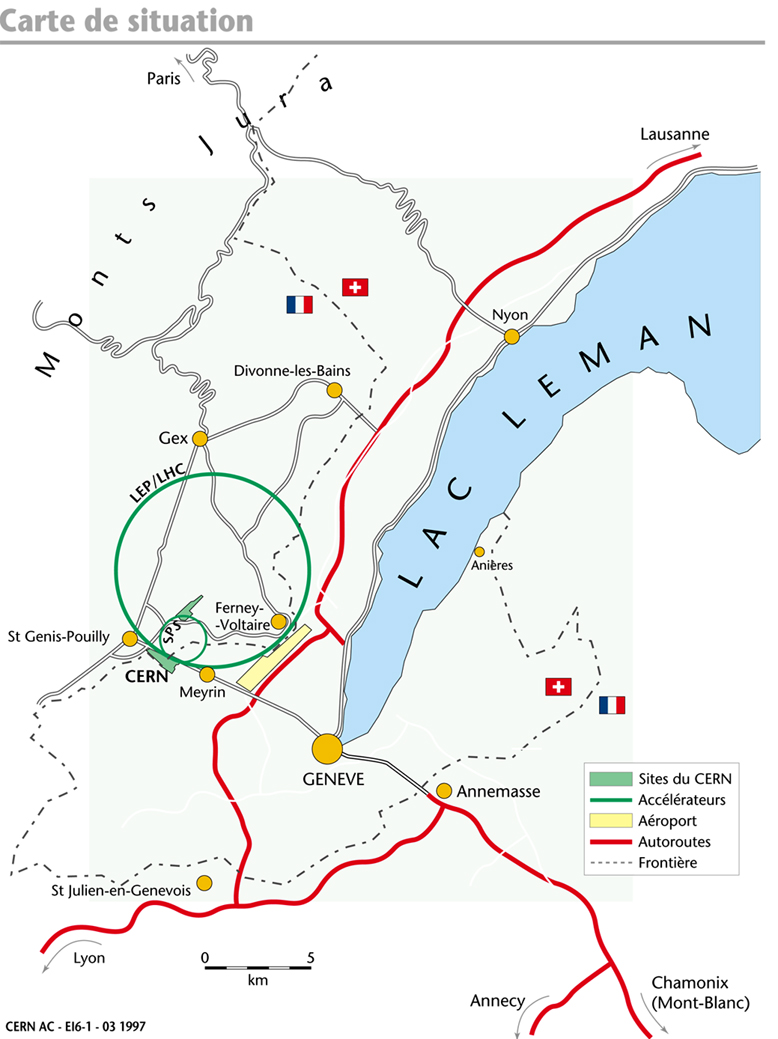
\includegraphics[width=0.6\textwidth]{Chapters/01_Introduction/Images/lhc-pho-1997-169.jpg}\\
     \caption{Map of LHC location.}
     \label{fig:LHC_map}
\end{figure}

This thesis presents an analysis based on the full proton-proton collision data from the CMS experiment in
2011 and 2012. The analysis investigates the top-antitop (\ttbar) differential cross section with respect to
global level event variables, specifically in semileptonic \ttbar decays in the electron+jets and muon+jets
channels. This investigation is motivated primarily by the importance of understanding \ttbar events, since
they are a significant background in many new physics analyses. The understanding of QCD and event generators
that studies such as this provide is also helpful for other physics analyses. Furthermore, rare Standard Model
processes such as $\ttbar + W\rightarrow l\nu$ or $\ttbar + Z\rightarrow \nu\bar{\nu}$ would appear in \met
distribution tail, and $\ttbar + X$ where $X$ is massive would appear in the \HT and \st distributions. There
are also possible new physics scenarios such as stop pair production, $\tilde{t}\bar{\tilde{t}} \rightarrow
t\tilde{\chi_0} \bar{t}\bar{\tilde{\chi_0}}$ which could show hints of dark matter.

The work presented here was carried out in collaboration with Emyr Clement, L{}ukasz Kreczko, Sergey Senkin
and Philip Symonds under the supervision of Professors Joel Goldstein and Greg Heath. The main contribution of
the author to these studies lay in development of the C++ and Python software frameworks and scripts used in
the analyses. Related to this, maintaining up-to-date particle object definitions, corrections, efficiencies
and prescription recommendations from working groups within CMS was a large component of the author's work. In
terms of the technical workflow employed, the author was heavily involved in producing n-tuples from the
analysis-ready AOD data format, running the software to perform the prescribed analysis methods, and running
final scripts on the output ROOT data to perform the final calculation and to produce results plots and
tables. Particular areas of focus regarding physics included synchronisation of the event selection,
comparison of distribution shapes between 7\TeV and 8\TeV data, and implementing aspects of the analyses such
as selection criteria, \btagging and jet energy resolution.

Chapters~\ref{c:CMS_Detector} and \ref{c:CMS_computing_and_offline} describe the LHC and the CMS detector,
including information about the object reconstruction process based on detector readout, to represent
particles produced in collisions. Chapter~\ref{c:the_standard_model} provides an overview of the Standard
Model theory and some of its shortcomings, followed by a review of physics of the top quark at the LHC in
Chapter~\ref{c:top_physics_at_the_lhc}. A small study investigating the \btagging algorithms used in CMS is
described in Chapter~\ref{c:b_tagging_study}, and the main \ttbar differential cross section analysis is then
covered in Chapters~\ref{c:Differential_Cross_Section:data_simulation_and_selection},
\ref{c:Differential_Cross_Section:fitting_unfolding_and_measurement}
and~\ref{c:Differential_Cross_Section:systematics_and_results}. To conclude, Chapter~\ref{c:summary} contains
a summary and outlook to the future. Additional data, tables and plots from the presented analyses are given
in Appendices~\ref{ac:b_tagging_plots} and \ref{ac:ttbar_diff_cross_section_analysis}. Finally, an addendum
describing the brief continuation of work from the author's MSc in testing a readout chip for the CMS strip
tracker is outlined in Appendix~\ref{ac:cbc}.

From the outset, natural units are used throughout this thesis, unless otherwise specifed, so that
\begin{equation}
\hbar = c = 1,
\end{equation}
meaning that mass, momentum and energy all have the same units of electronVolts (eV).
\chapter{The CMS Detector at the LHC}
\label{c:CMS_Detector}

\section{Introduction to the LHC}
\label{s:Introduction}
The CMS general-purpose detector is one of four detectors located around the LHC, approximately 100\m below
ground level. The CERN accelerator complex and the locations of the various experiments around the LHC are
shown in Figure~\ref{fig:LHC_schematic}.

\begin{figure}[hbtp]
   \centering
     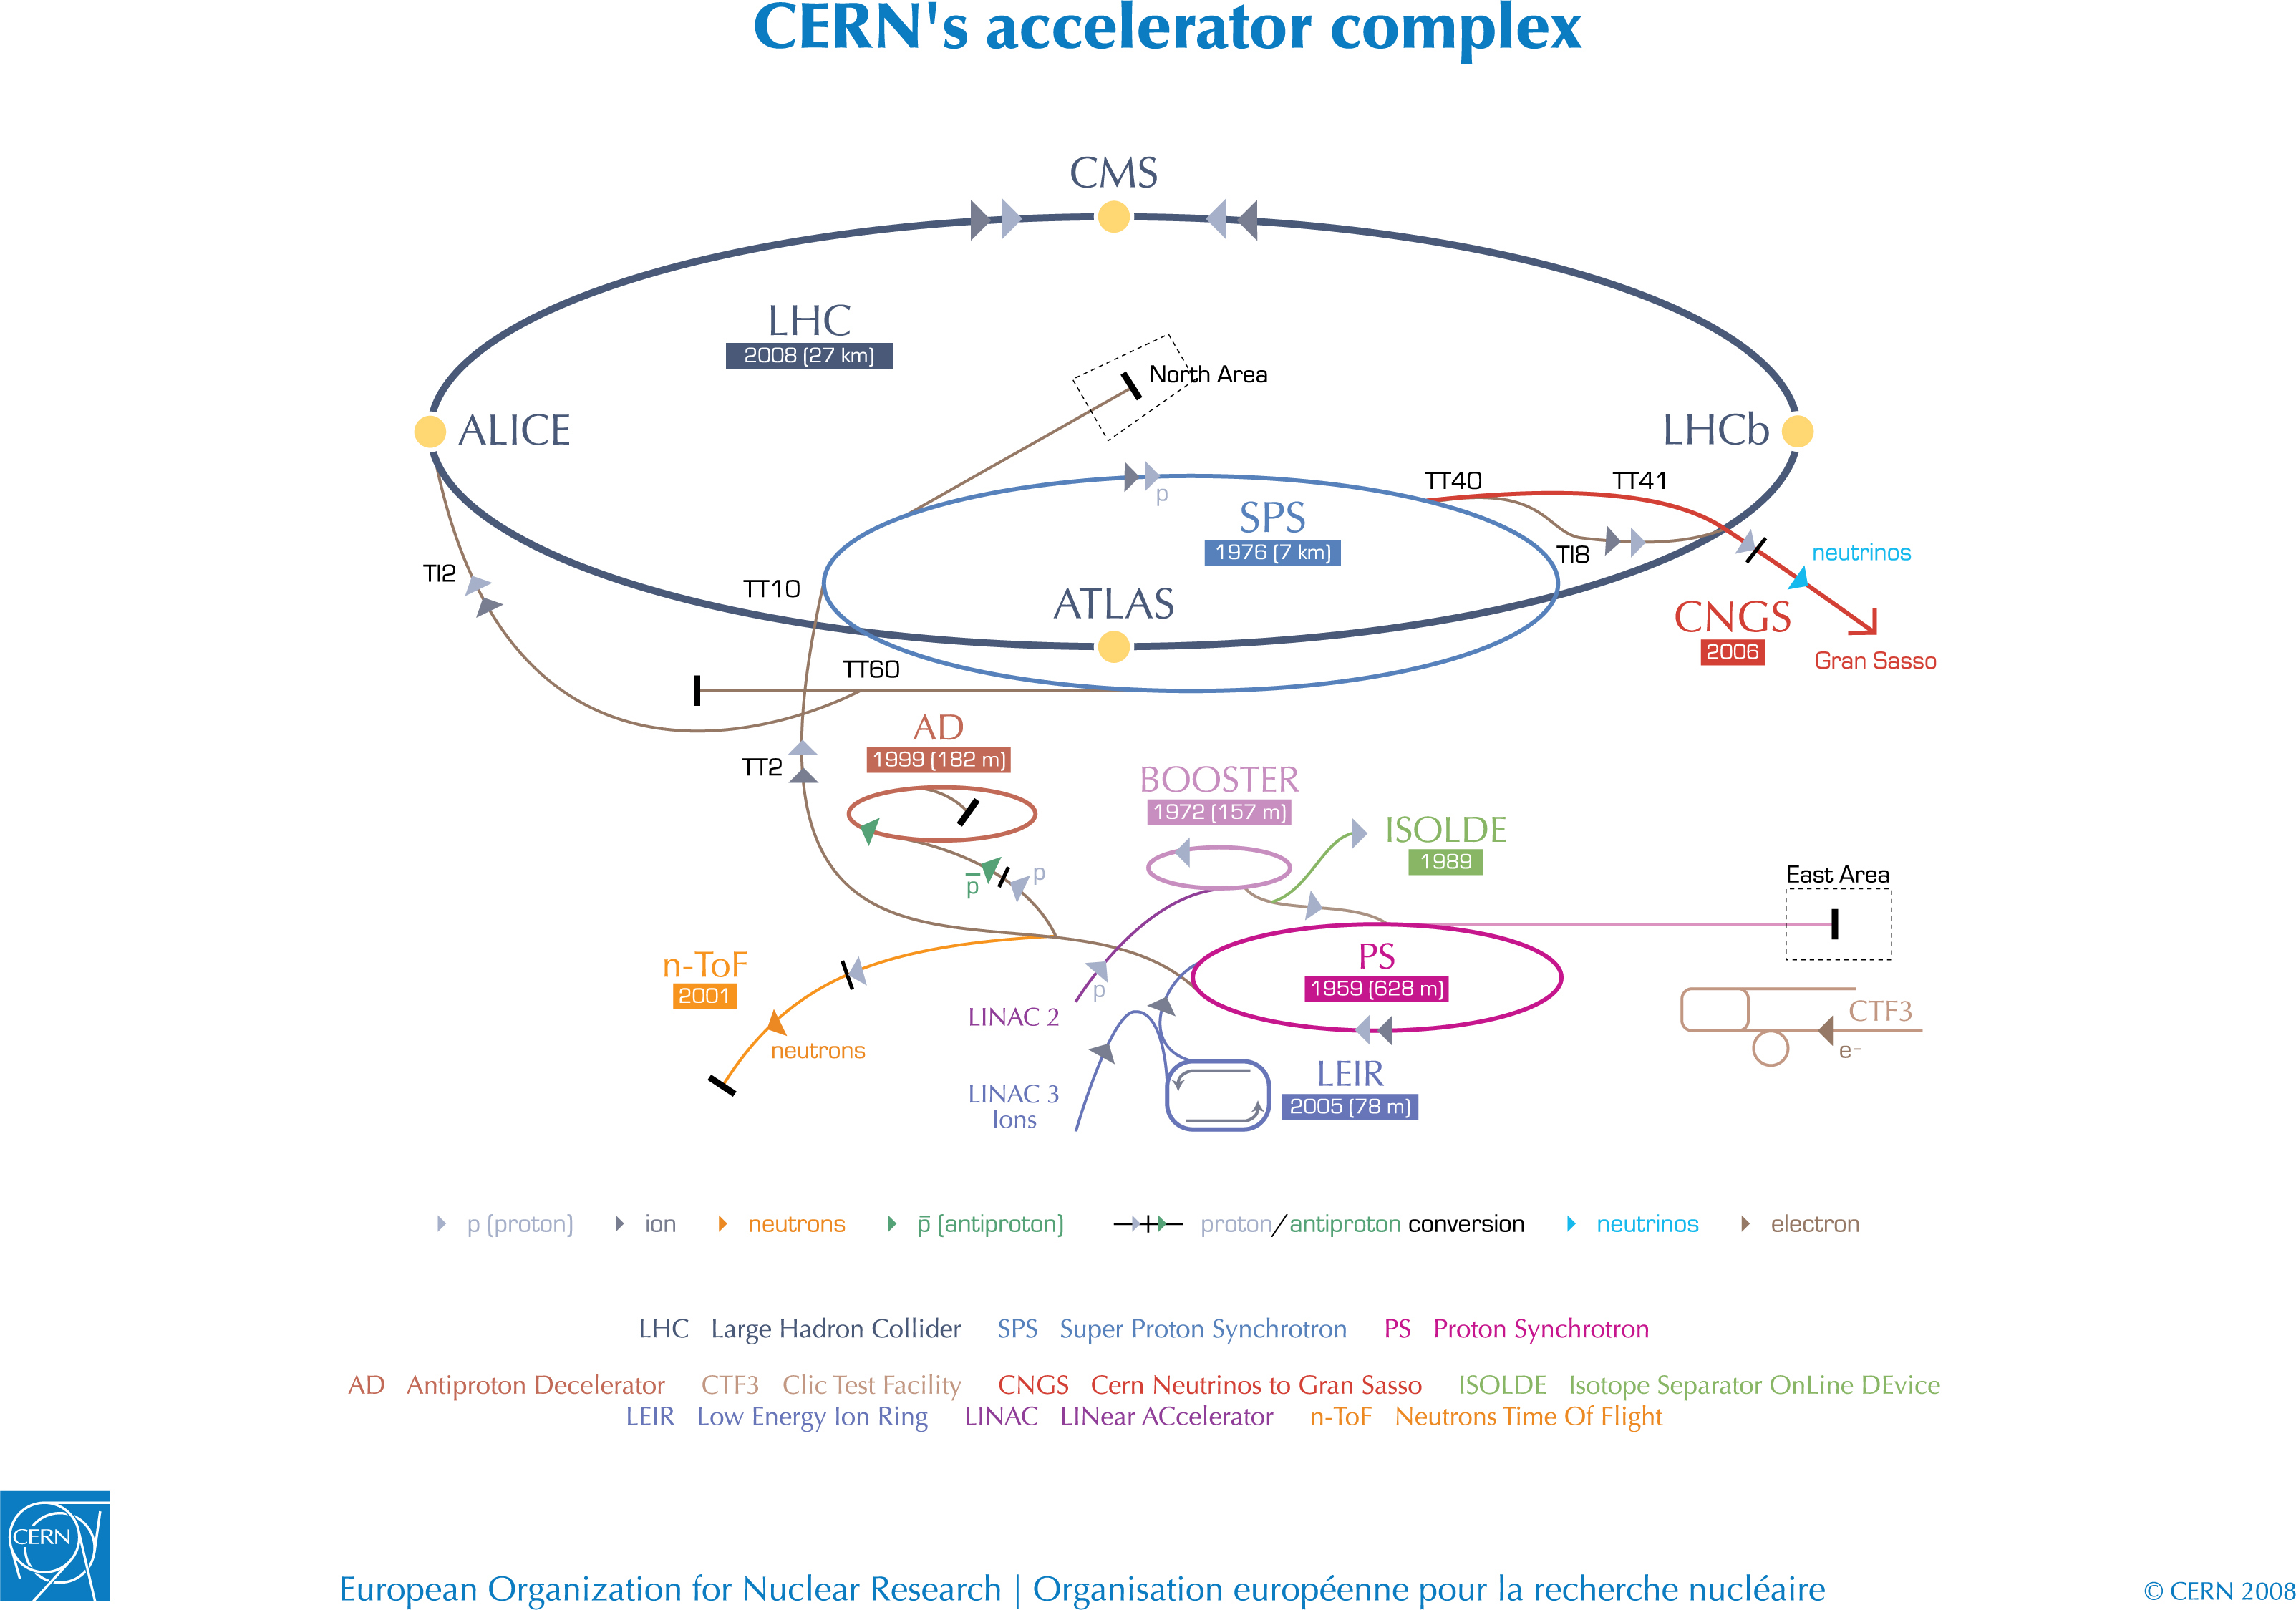
\includegraphics[width=\textwidth]{Chapters/02_Detector/Images/0812015.jpg}\\
     \caption[Schematic of LHC and experiments.]{Schematic of CERN accelerator complex including the LHC and
     experiments.
     CMS is located at Point 5 on the LHC ring.}
     \label{fig:LHC_schematic}
\end{figure}

The 27\km circumference LHC can collide two proton beams, each composed of 2808 bunches, at a design energy of
7\TeV per beam (meaning a 14\TeV centre of mass energy, \roots, in collisions) with a luminosity $\mathcal{L}$
of $10^{34}\cm^{-2}\s^{-1}$ at a collision rate of 25\ns (40~\MHz). Each event that is recorded in the CMS
detector is one crossing of the bunches of protons of which the beams are comprised. During the first part of
Run 1 in 2011 the machine ran at a centre of mass energy of 7\TeV at a bunch spacing of 50\ns (leading to 8
proton-proton interactions per bunch crossing) and CMS recorded a peak instantaneous luminosity of
$3.7\times10^{33}\cm^{-2}\s^{-1}$. In 2012 the centre of mass energy was increased to 8\TeV (21 proton-proton
interactions per bunch crossing) and CMS recorded a peak instantaneous luminosity of
$7.7\times10^{33}\cm^{-2}\s^{-1}$. Since Run 2 began in May 2015 after Long Shutdown 1, the LHC has been
operating at a collision energy of 13\TeV and CMS recorded a peak instantaneous luminosity of
$4.7\times10^{33}\cm^{-2}\s^{-1}$ at a collision rate of 25\ns initially, before switching to 50\ns.
The design collision energy and luminosity are scheduled to be attained later in Run 2 and after Long Shutdown
2 (in 2019) respectively. 6.1\fbinv and 23.3\fbinv of data was delivered to CMS during the 2011 and 2012 data
taking periods respectively; Figure~\ref{fig:integrated_luminosity} shows the increase in integrated
luminosities delivered to CMS over time during 2010$--$2012.

The acceleration process begins with a tank of hydrogen (see Figure~\ref{fig:LHC_schematic}). After stripping
electrons off the hydrogen atoms using an electric field, the remaining protons are inserted into the Linear
Accelerator 2 (LINAC2) which accelerates them up to 50\MeV. From here, the proton beam is injected into the
Proton Synchrotron Booster (PSB) which increases the energy to 1.4\GeV, followed by the Proton Synchrotron
(PS) which accelerates the beam to 25\GeV and the Super Proton Synchrotron (SPS) where the beam energy reaches
450\GeV. Finally, the protons are injected into the LHC where two beampipes carry the beams in a clockwise and
an anti-clockwise direction while accelerating them up to the required collision energy. Filling the LHC rings
takes approximately 4 minutes, followed by approximately 20 minutes until the beams reach energies of 4\TeV
(during 2012 data taking). The beams are accelerated by radio frequency cavities, and superconducting dipole
magnets bend the beams to maintain their trajectory around the LHC beampipe. Once the collision energy has
been attained, the beams are ``squeezed'' to focus them into a cross sectional area of approximately 16\um
using superconducting quadrupole magnets. Collimators act to scrape away protons, thereby maintaining beam
losses to the superconducting magnets below the level that would cause quenching. The counter-circulating
beams are brought to collide at the four main LHC experiments CMS, ATLAS, LHCb and ALICE. ATLAS, like CMS, is
a general purpose detector, ALICE is specifically designed to investigate heavy ion collisions (as opposed to
protons), while LHCb investigates b-meson physics.

\begin{figure}[hbtp]
   \centering
     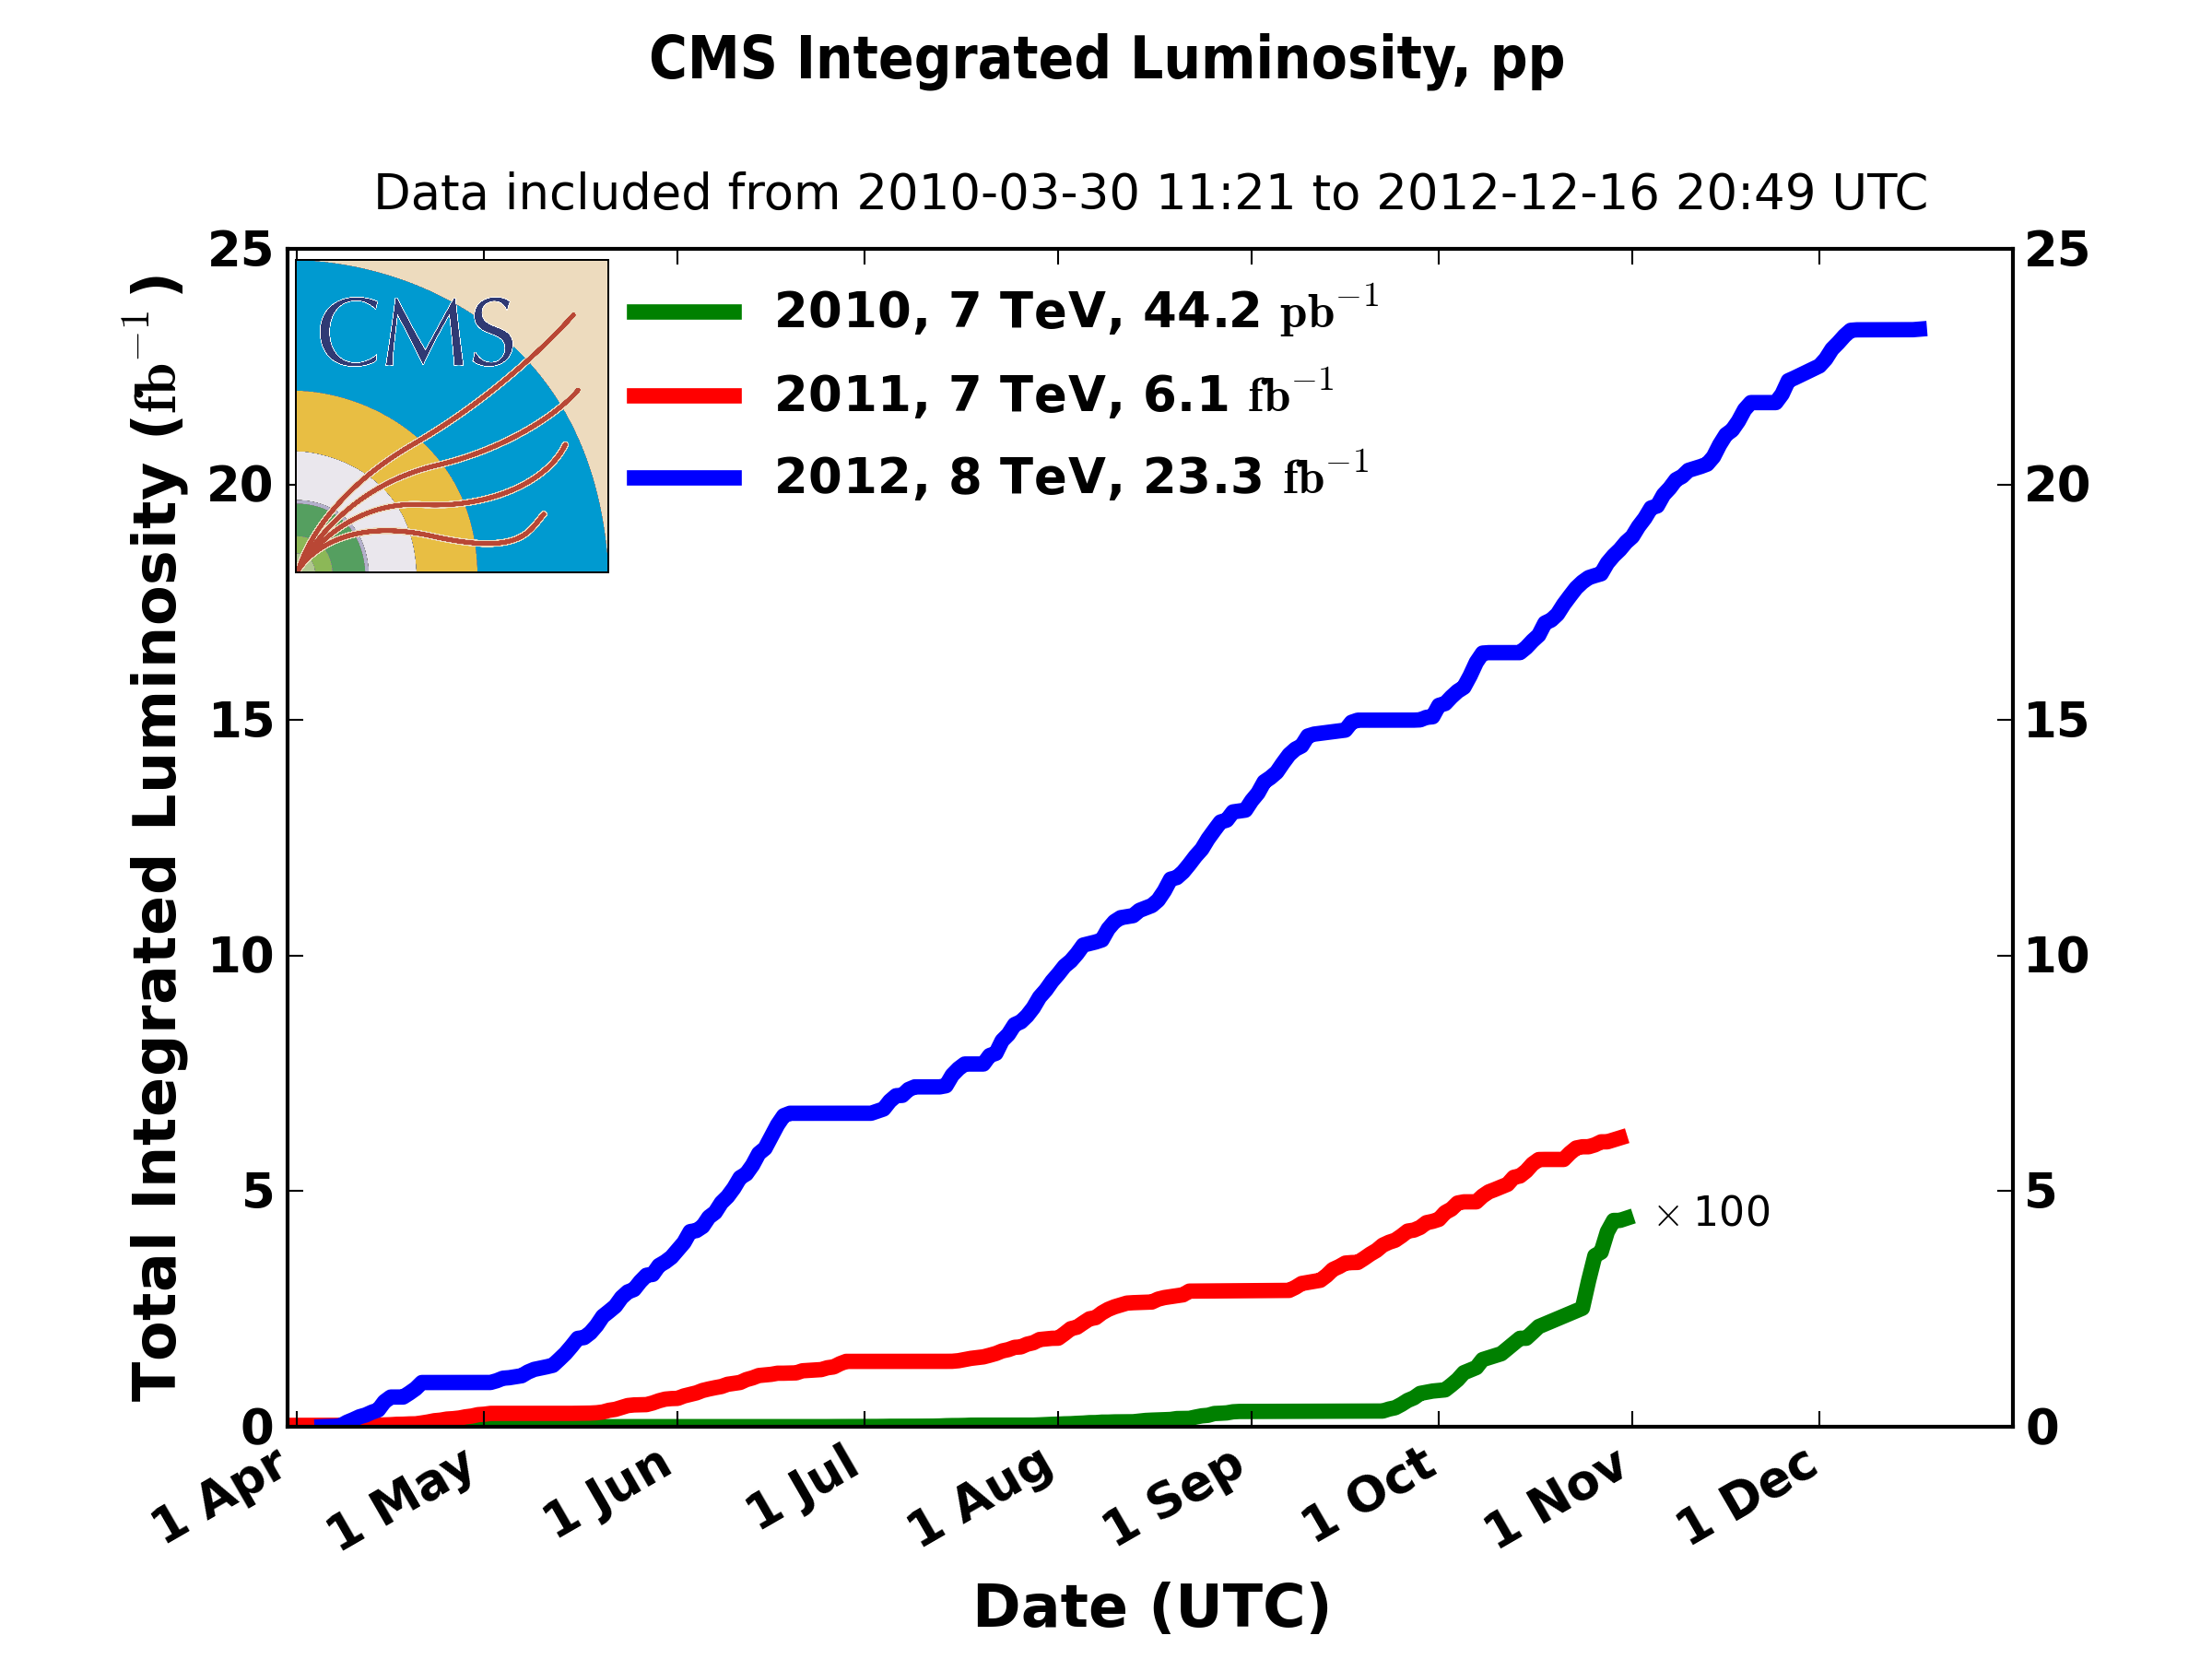
\includegraphics[width=0.75\textwidth]{Chapters/02_Detector/Images/int_lumi_cumulative_pp_2.png}\\
     \caption[Cumulative luminosity delivered to CMS during 2010, 2011 and 2012.]{Cumulative luminosity
     delivered to CMS over time during 2010, 2011 and 2012 proton-proton data taking periods.}
     \label{fig:integrated_luminosity}
\end{figure}

\section{Overview of CMS}
\label{s:Overview}
Compact Muon Solenoid is both the name of the detector at the LHC, and of the collaboration of people
worldwide who work to build, operate, maintain and upgrade it, and to analyse the data it records.

CMS is a general-purpose detector, designed to be efficient at detecting new physics with a wide range of
signals. The detector measures 14.6\m in diameter and 21.6\m in length, and weighs 12500~tonnes
\cite{CMS_experiment}. The different sub-detectors of CMS are arranged in concentric layers around the point
of the beampipe at which the two beams of proton bunches collide, known as the interaction point (see
Figure~\ref{fig:CMS_diagram}). As the products of any collisions that occur in the bunch crossing travel
outwards from the interaction point, they pass through the sub-detectors depositing energy, resulting in
signals being produced. A subset of the information from some sub-detectors (the calorimeters and muon
chambers, described in Section~\ref{s:Subdetectors}) is then processed by a trigger while information from
other sub-detectors is buffered on the detector.

\begin{figure}[hbtp]
   \centering
     \includegraphics[width=\textwidth]{Chapters/02_Detector/Images/cms_120918_02.pdf}\hfill
     \caption[Diagrammatic sectional view of the CMS detector.]{Diagrammatic sectional view of the CMS
     detector
     \cite{Sakuma_sketchup}.}
     \label{fig:CMS_diagram}
 \end{figure}

The design of CMS is based firstly around a superconducting solenoid magnet. Around and inside the magnet are
the sub-detectors: the pixel and strip tracker, the electromagnetic calorimeter, the hadronic calorimeter, the
return yoke for the magnet and the muon detectors. The coordinate system of the detector is designated with
the origin as the intersection point of the two beams in the beampipe, the x-axis positive towards the centre
of the LHC ring, the y-axis positive vertically upwards and the z-axis pointing along the beampipe in an
anticlockwise direction. The azimuthal angle, $\phi$, is defined as the angle in the x-y plane, transverse to
the beampipe starting from the x-axis. The polar angle, $\theta$, is defined as the angle in the z-y plane
starting from the z-axis (the beampipe). The angle $\theta$ is related to the pseudorapidity, $\eta$, by the
formula $\eta=-\ln(\tan(\theta/2))$, so that $\eta$ ranges from 0 at $\theta=90~\degreeCelsius$ to $\infty$ at
$\theta=0~\degreeCelsius$~\cite{CMS_TDR1}. The two ends of the detector, at high $\abseta$ values, are called
the endcap regions while the central area at lower $\abseta$ values is called the barrel region. The detector
volume is often denoted in terms of $\Delta R$, with the separation between two particles 1 and 2 being
defined as

\begin{equation}
\Delta R = \sqrt{(\eta_{1} - \eta_{2})^{2} + (\phi_{1} - \phi_{2})^{2}}
\end{equation}

\section{Sub-Detectors}
\label{s:Subdetectors}

\subsection{Tracker}
\label{ss:Tracker}

Any charged particles produced as a result of the proton-proton collisions in these bunch crossings need to be
recorded for later use in reconstruction of particle information such as trajectories and charges. This is
achieved using the tracker section of CMS which consists of silicon sensors in two forms: pixels and strips.
As the charged particles travel through these silicon sensors, electron-hole pairs are produced that induce a
current in the sensors and are processed by readout chips. This readout is carried out by the Analogue
Pipeline Voltage 25 (APV25) chip. A new chip called the CMS Binary Chip (CBC) is intended to replace the APV25
in the HL-LHC after Long Shutdown 3, currently scheduled for 2023-2024. The CBC is described in more detail in
Appendix~\ref{ac:cbc}.

The purpose of the tracker within the CMS detector is to track the trajectory of charged particles as they
travel out from the interaction point. An important requirement of the tracker is that it must allow the above
whilst not affecting the energy of the particle being tracked. The silicon in the tracker sensors also does
not stop particles, thereby allowing them to pass through this innermost layer of the detector and interact
with outer layers. The tracker readout chips must also be able to distinguish from which bunch crossing a
particle was produced (bunch-crossing identification) in order for the trigger to remove particles from
previous bunch crossings (termed out-of-time pileup) and fully reconstruct events.

The tracker is split into two parts, with an inner silicon pixel detector and an outer silicon strip detector.
A diagrammatic view of the tracker, including both pixels and strips, is shown in
Figure~\ref{fig:CMS_strip_tracker}. The inner pixel detector consists of three layers in the barrel region at
distances of 4.4\cm, 7.3\cm and 10.2\cm from the beam line with two endcap discs at each end. Each pixel
measures 100\um by 150\um. The entire pixel detector covers an area of only approximately $1\m^{2}$ but
contains 66~million pixels in total.

The strip tracker is comprised of ten layers in the barrel region at distances ranging from 20\cm to 1.1\m
from the beampipe. The four inner layers (at distances of 26\cm, 34\cm, 42\cm and 50\cm from the beampipe)
are collectively named the Tracker Inner Barrel (TIB), while the outer six layers (at distances of 61\cm,
70\cm, 78\cm, 87\cm, 97\cm and 108\cm from the beampipe) are known as the Tracker Outer Barrel (TOB).
The endcaps consist of twelve discs, three of which correspond to the Tracker Inner Discs (TID) at z-distances
from 75\cm to 100\cm, and nine to the Tracker End Caps (TEC) at z-distances between 120\cm and 280\cm
\cite{Palmonari:1260970}. The largest silicon detector ever constructed, the strip tracker contains about ten
million channels and covers an area of approximately $200\m^{2}$ \cite{CMS_experiment,CMS_TDR1}. The operating
temperature of the tracker during 2011 and 2012 has been $0~\degreeCelsius$ for the pixels and
$+4~\degreeCelsius$ for the strips but will be lowered for both after Long Shutdown 1~\cite{Butz:1497745}.

\begin{figure}[hbtp]
   \centering
     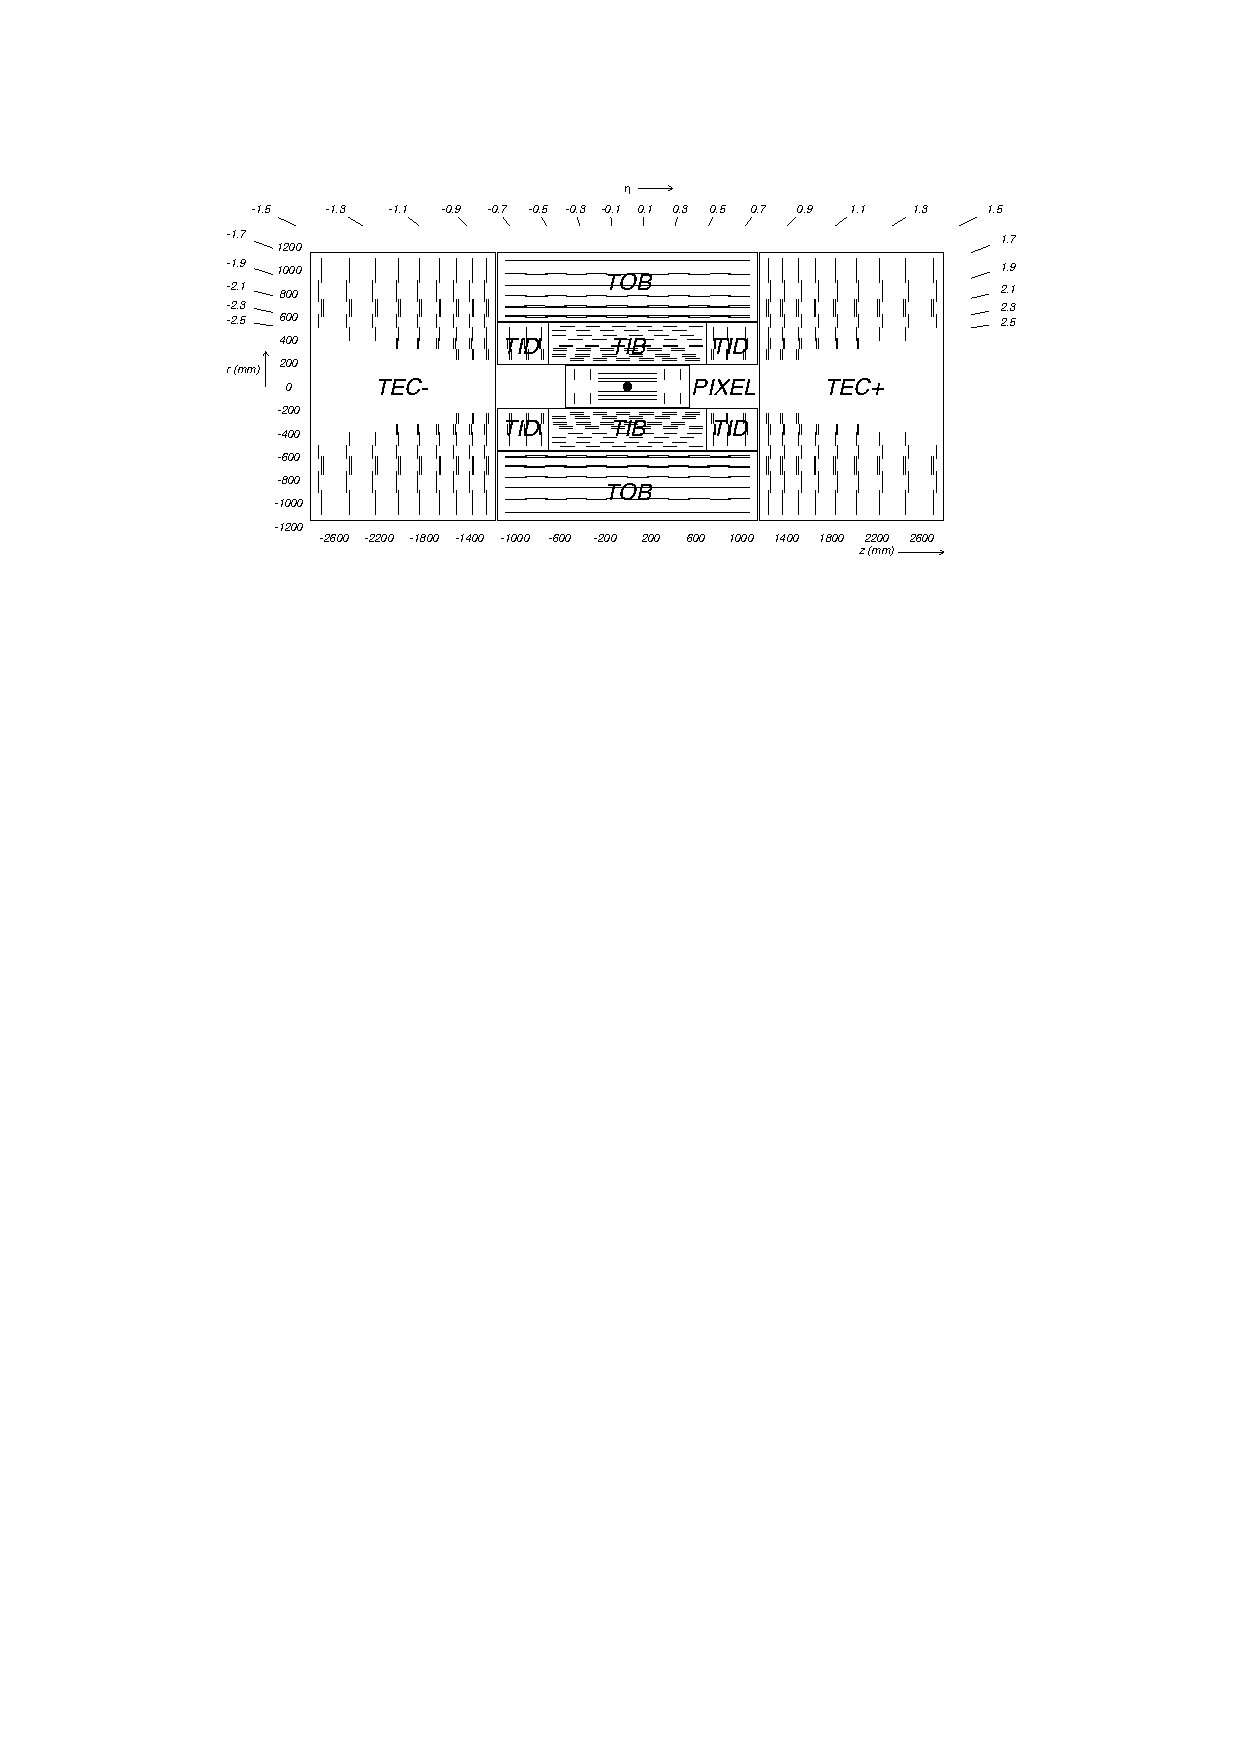
\includegraphics[width=\textwidth]{Chapters/02_Detector/Images/tracker.pdf}\hfill
     \caption[Cross sectional diagram of the CMS strip tracker.]{Cross sectional diagram of the CMS strip
     tracker; each line represents a detector module
     \cite{CMS_TDR1}}
     \label{fig:CMS_strip_tracker}
\end{figure}

As a charged particle passes through the various layers of silicon in these detectors, electrical signals are
created which are then read by readout electronics. Offline algorithms then use the data relating to which
strips and sensors received `hits' to reconstruct the tracks of charged particles and this information is
later used for particle reconstruction and identification \cite{CMS_experiment,CMS_Tracking_Early_Results}.

% Neutral particles could also leave signals in the tracker in a small proportion of cases if the particle
% interacts with a silicon atom and/or converts to charged particles such as a photon conversion to two
% electrons. In the majority of cases, the presence of neutral particles must be detected from their energy
% deposits in the calorimeters.
The curving of particle tracks within a magnetic field allows the calculation of the particle momentum and
charge, $mv=RqB$, where $mv$ is the momentum of the particle, $R$ is the radius of curvature, q is the
electric charge, and B is the magnetic field strength.

%With the higher data rate expected after the LHC upgrades over the coming decade,
%pile-up will become an important issue, with approximately 20 interactions per bunch crossing even at the
%current design luminosity. This number is expected to increase to 100-200 following Long Shutdown 3.

%At higher luminosities, the occupancy (the fraction of channels with a 'hit') increases,
%which makes pattern recognition more difficult for track reconstruction algorithms and readout systems. The
%higher tracker resolution desirable for such circumstances also requires more sensors and readout chips. As a
%result, any new chip would need to be more efficient in its use of power whilst processing the data and/or
%require the associated cooling systems to be more efficient. Indeed, studies have shown that the present
%tracker could itself produce acceptable tracking performance in such conditions based on simulations of
%heavy-ion collisions, which produce similar numbers of tracks per event to that expected after the luminosity
%upgrades at the LHC [10].

%The LHC upgrades are split into 2 phases. The pixel detector will be upgraded during Phase 1, and will be an
%on-going process during both Long Shutdown 1, Long Shutdown 2 and shorter intermediate shutdowns. The strip
%detector will be upgraded during Phase 2, more specifically during Long Shutdown 3 [11][12].

The required tracker characteristics of high granularity and resolution, fast response to process the high
data rate without losing potentially valuable information, radiation hardness and keeping detector material to
a minimum to minimise interactions of the particles with detector matter, resulted in silicon being chosen to
construct the tracker.

One of the advantages of using silicon over gaseous detectors is that silicon produces more charge carriers
per unit of length travelled by a particle. This therefore means the silicon thickness can be reduced,
typically around 300\um per layer. The silicon sensors that make up the strip tracker in the CMS detector vary
in thickness depending on their location. Sensors of 320\um thickness are utilised in the TIB and TID, 500\um
in the TOB, and a mixture of both thicknesses is used in the TEC. Thicker sensors are used in the outer
sections of the strip tracker in order to maintain a high signal to noise ratio, since the increased strip
lengths in this region lead to increased electronics noise due to higher capacitance~\cite{CMS_experiment}.

Silicon also allows fast signal transfer, of the order of about 10\ns, as the charge carriers travel quickly
through silicon. Furthermore, the spacing between strips in a silicon sensor, known as the strip pitch, can be
manufactured to be extremely small, down to around 50\um. The strip pitches and their lengths vary such that
there are fifteen distinct types of sensor geometries in the strip
tracker~\cite{Commissioning_and_Performance_Strip_Tracker}.

A further tracker requirement is low occupancy (the fraction of channels with a hit in an event was desired to
be 1~\% or lower at the nominal LHC luminosity) so that pattern recognition can be carried out efficiently and
so the amount of simultaneous data to be read out is manageable. In order to maintain such a low occupancy,
the strip tracker has a high granularity, with strip lengths less than 20\cm and strip pitches less than
205\um~\cite{Palmonari:1260970}. While high granularity is beneficial for high precision tracking, it also
results in a high number of channels, which in turn requires a large amount of electronics for readout and
leads to a high heat load.

On a global scale, the tracker data is read out using a combination of interoperating systems.
The data from the APV25 tracker readout chips is taken via optical fibres to 440
off-detector Front End Drivers (FEDs) (tracker FEDs make up 63~\% of the total number of FEDs in CMS).
The FEDs then forward the data to the online Data Acquisition System (DAQ). In addition, off-detector Front
End Controllers (FECs) control the front-end electronics by means of approximately 350 control rings,
including triggers, clock and monitoring~\cite{CMS_experiment, Corrin}.

%As a result of the higher collision rates to be expected after
%these upgrades, the CMS tracker will require an improvement in its infrastructure because of radiation damage
%it will have suffered by that point and to ensure that it is robust enough to handle the higher levels of
%radiation after the upgrades. The pile-up is also expected to be in the range of 100 to 200 interactions per
%bunch crossing which also necessitates an improvement in the CMS tracker performance in order to ensure
%valuable data are not lost during collisions \cite{CMS_Silicon_Tracker_upgrade_for_HL-LHC}.

% Within the lattice of pure silicon, there are well-defined bands of energy levels called the conduction band
% and the valence band. The band gap is the difference in energy between these two bands and varies depending on
% the material. At absolute zero, -273$^{\circ}$C, almost all the electrons can be said to be fixed in place in
% this lattice in the valence band, meaning that if an electric field is applied across the silicon, no current
% would be able to flow. When energy is input to the system and an electron gains energy, it may be able to
% cross the band gap to the conduction band, in which case a hole would be present in its previous place in the
% valence band. At this point, both the electron and the hole are mobile and can move freely in current flow,
% for example, under the influence of an electric potential. Materials with a large band gap are insulators, and
% those with a small band gap (or even sometimes with energy bands that overlap with each other) are conductors.
% Silicon, being a semiconductor, has a 'medium' sized band gap of approximately 1.12eV. Nevertheless, the
% number of mobile electrons, above absolute zero, is still large enough to make it difficult to distinguish the
% real signal from the inherent noise in the silicon, known as leakage current (explained in Section 2.3.2).
% In order to decrease this number of free electrons and holes in silicon to obtain a much cleaner signal from a
% traversing particle (i.e. improve the signal to noise ratio), a process called doping is employed to increase
% the number of charge carriers. This involves the substituting of silicon atoms in the lattice with atoms of
% other elements like arsenic, phosphorous, boron or aluminium. In the case of the former two, both have five
% valence electrons. Four of these electrons bond to the four valence electrons present in a silicon atom,
% leaving one electron that can be easily removed from the lattice to the conduction band. This 'donation' of
% electrons to the conduction band increases the number of charge carriers. This type of silicon is called
% n-type silicon because the additional charge carriers are negative. Similarly, if boron or aluminium atoms are
% introduced to the silicon lattice, their three valence electrons bond to the electrons in a silicon atom but
% one silicon electron has nothing to bond to, creating a mobile positive hole. The addition of holes (which
% 'accept' electrons) leads to this type of silicon being called p-type because the additional charge carriers
% are positive.
% Although both p- and n-type silicon increase the number of free charge carriers, a PN-junction can be created
% by attaching a piece of n-type silicon to a piece of p-type silicon. Considering a PN-junction in isolation,
% mobile electrons from the n-type silicon would diffuse into the p-type silicon and unite with the holes from
% the p-type material, leaving behind the positively charged donor atoms. Similarly, the mobile holes from the
% p-type silicon would diffuse to the n-type silicon and leave behind negatively charged acceptor atoms. As
% these electrons and holes move to the two sides of the junction, the resulting electric field opposes the
% initial diffusion of electrons and holes, eventually reaching a state of equilibrium. Once equilibrium is
% reached, this area around the PN-junction will contain no mobile charge carriers and is called the depletion
% region.
% However, if a reverse bias voltage is applied to the silicon (a negative terminal connected to the p-type
% silicon and a positive terminal to the n-type silicon), then the electrons from the n-type silicon, rather
% than diffusing towards the junction, will be attracted towards the positive terminal. Similarly, the holes
% from the p-type silicon will be attracted towards the negative terminal, as shown in Figure 7.
% 
%  
% A higher reverse bias voltage leads to a larger depletion width as more electrons and holes are carried away
% from the junction. At high enough voltages, the width of the depletion region can be made equal to the width
% of the silicon; this voltage is known as the depletion voltage. At this stage, there are no free charge
% carriers anywhere in the silicon and it is in this state that silicon detectors are operated, thus ensuring
% that any charge carriers are only produced as a charged particle travels through the silicon. In this state,
% silicon detectors are effectively reverse biased diodes, only allowing a current to flow in one direction.
 
%Figure 8 - Basic diagram of silicon strip detector with p+ strips (green) on n-bulk (blue) [24].

% The silicon sensors in the CMS strip tracker are p+ strips (which denotes a high concentration of p-type
% impurities) on n-bulk sensors, similar to the diagram in Figure 8. As the silicon is ionised by a traversing
% particle, mobile charge carriers are created which then travel, due to the depletion voltage, to the p+ strips
% (holes) or to the backplane (electrons). As the signal will be created on a particular strip (or strips), it
% will then be possible to deduce the position of the particle.

% 2.3.2 Radiation Hardness The current tracker front-end electronics were initially designed to last about 10
% years in operation under the radiation conditions of the detector [5]. The higher radiation they will be
% subjected to as a result of the higher luminosity and higher collision energies at the HL-LHC will clearly
% impose the requirement that all components, including sensors and electronics, should be manufactured to a
% higher standard of radiation hardness. Radiation damage can occur when particles of high enough energy are
% created in the collisions at the centre of CMS that when they pass through the silicon tracker, they collide
% with atoms in the lattice. This damage is done most often by neutrons, in particular low energy neutrons from
% calorimeters and other detector elements, which interact with nuclei in the silicon and move atoms out of
% place. These atoms are knocked out of place into levels where there is usually no atom, known as interstitial
% levels. An energy of around 15eV is necessary for this to happen; generally at energies of 2keV or less only
% isolated displacements occur, whereas for energies between 2 and 12keV, one or more defect clusters will be
% created. The removal of donor atoms in this way leads to a change in the doping concentrations and eventually
% to an increase in the leakage current (current which may flow when there is no ionising particle traversing
% the silicon). A leakage current will in turn require a higher depletion voltage to remove additional electrons
% or holes captured by the electronically active defects.
% The leakage current is temperature dependent and can be mitigated by using low temperatures. The planned
% running temperature of the CMS silicon tracker in the HL-LHC is planned to be lowered from +4$^{\circ}$C to
% the region of -20$^{\circ}$C to -40$^{\circ}$C due to the benefits in terms of radiation damage. To evaluate
% the behaviour of the proposed CBC in these conditions, an environmental chamber was used to carry out tests at
% varying temperatures in this project. If a leakage current is present, this will lead to noise in the system,
% since current will always flow and any signal would sit on top of this noise. If subject to high levels of
% radiation damage, the leakage current increases to levels at which excessive amounts of power are dissipated,
% and the noise in the readout will be too high to read a clean signal.
% 
% 2.3.3 Noise The aforementioned leakage current is a result of the quantised nature of the charge carriers.
% This noise is present even when there is no signal present, and increases as radiation damage increases the
% leakage current.
% Other potential sources of noise include electronic noise caused by thermal fluctuations of the charge
% carriers. This would manifest as noise in the amplifier at the front end of the CBC and would increase
% proportionally with the capacitance of the connected input system [25]. Another contributor to noise in the
% system could be from non-linearity of the analogue to digital converter (ADC) in the CBC that converts the
% incoming analogue pulse to a digital signal [25].
% The dominant source of noise in our test system is likely to have resulted from electronic noise in the
% connected laboratory setup. In practice, the external noise under operational conditions when the CBC is
% connected to the CMS detector should ideally be maintained lower than the noise in the amplifier.


\subsection{Electromagnetic Calorimeter}
\label{ss:Ecal}
The electromagnetic calorimeter (ECAL), is a hermetic, homogeneous sub-detector constructed of scintillating
crystals of lead tungstate ($\mathrm{PbWO_{4}}$), and is the next layer outside the tracker. Any
electromagnetic particles such as electrons or photons are absorbed by the ECAL crystals which then
scintillate emitting a blue-green coloured light. These signals are then collected and converted to electrical
signals by connected photodetectors, and processed by readout electronics.

The signals in the crystals are collected by avalanche photodiodes in the barrel region and vacuum
phototriodes in the endcaps. The numbers of photoelectrons produced is dependent on temperature, with
increasing temperature resulting in a decrease in the number of electrons at a rate of
$-3.8\pm0.4\%/\degreeCelsius$. A cooling system is thus employed which maintains a stable operating
temperature of the ECAL system to within $\pm0.05\degreeCelsius$, with a nominal operating temperature of
$18\degreeCelsius$~\cite{CMS_experiment}. The energy resolution of the ECAL has been shown to follow
$\sigma_{E}/E = 2.8\%/\sqrt{E}\oplus 12\%/E \oplus 0.3\%$ where the three constant terms come from stochastic
fluctations such as photostatistics, electronics noise and temperature stability and calibration uncertainties
\cite{ECAL_calibration_and_resolution_at_7TeV}.

The barrel region of the ECAL consists of 61,200 crystals and extends up to a pseudorapidity $\eta\pm1.479$.
Each individual barrel crystal is $25.8X_{0}$ thick, where $X_{0}$ is the radiation length (the mean distance
over which a high energy electron loses all but 1/$e$ of its energy through bremsstrahlung
radiation~\cite{Agashe:2014kda}), and has cross sectional dimensions of $22\times22\mm^{2}$, which equates to
$0.0174\times0.0174$ in $\eta-\phi$ plane. These crystals are divided into 36 groups, called supermodules,
with each consisting of 4 smaller modules. The endcaps are comprised of 7,324 crystals, cover the range
$1.479\leq\eta\leq3.0$ and are split into two halves known as ``Dees", each divided into operating segments of
$40\degreeCelsius$ each. The endcap crystals have slightly larger dimensions, having a thickness of
$24.7X_{0}$ and cross sectional dimensions of
$28.62\times28.62\mm^{2}$~\cite{CMS_experiment,ECAL_frontend_monitoring}. Figure~\ref{fig:CMS_ECAL} shows the
layout of the ECAL.

The crystals of high density ($8.28~\g/\cm^{3}$), short radiation length ($X_{0}=0.89\cm$), and small
Moli\`{e}re radius (a measure of the transverse dimensions of electromagnetic showers in a
material~\cite{Agashe:2014kda}) of 2.2\cm lead to a compact calorimeter with fast response time (80~\% of the
light is emitted within 25\ns) and high granularity, capable of withstanding the radiation levels within CMS.

\begin{figure}[hbtp]
   \centering
     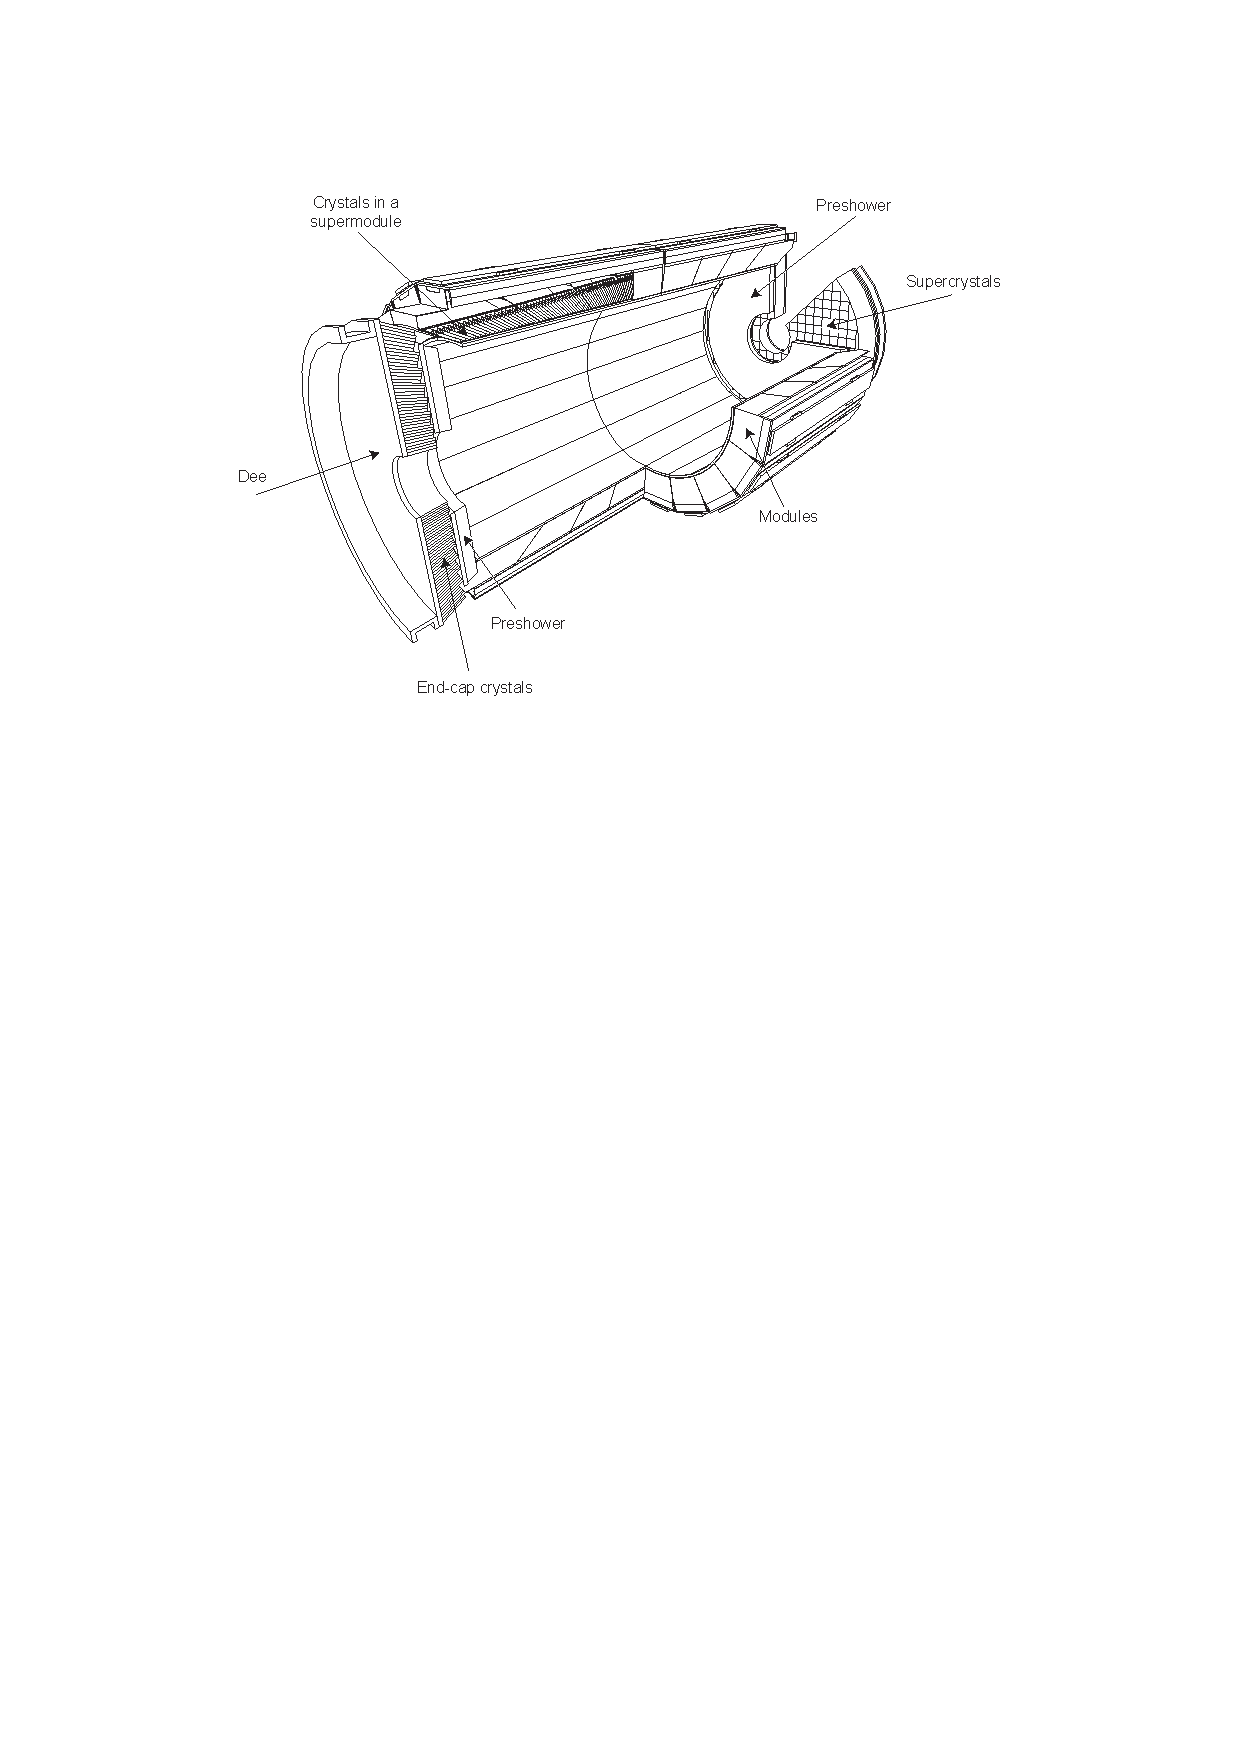
\includegraphics[width=0.7\textwidth]{Chapters/02_Detector/Images/ECAL.pdf}\hfill
     \caption[Diagram of the ECAL showing barrel supermodules, endcaps and preshower detectors.]{Diagram of
     the ECAL showing barrel supermodules, endcaps and preshower
     detectors~\cite{ECAL_calibration_and_resolution_at_7TeV}.}
     \label{fig:CMS_ECAL}
\end{figure}

An ECAL preshower, comprised of two lead plates each followed by a layer of orthogonal silicon strip sensors
(thickness 350\mm, strip pitch 2\mm) is located between the tracker and ECAL endcaps to provide a higher
spatial resolution than the ECAL. This helps to identify, for instance, closely spaced photon pairs
originating from pion decays which may otherwise be identified as a single high-energy photon based on ECAL
energy deposits. As photons pass through the lead, a shower of electromagnetic particles ($e^{+}e^{-}$ pairs)
is produced that are detected by the silicon layers to give a measure of the energy of the photon, while the
orthogonal strips allow a position measurement. The measured energy can then been combined with the energy
measured by the ECAL.

\subsection{Hadronic Calorimeter}
\label{ss:Hcal}
The next sub-detector outside the ECAL is the hadronic calorimeter (HCAL) which works in a similar way to
the ECAL, in this case by absorbing hadron jets. The HCAL is located at a distance of 1.77~m to 2.95~m from
the beamline, with an additional outer hadronic calorimeter also installed outside the magnet due to
radial restrictions imposed by the magnet coil. The HCAL barrel (HB), outer (HO) and endcaps (HE) cover
the $\abseta$ range up to 3.0, with the forward HCAL (HF) placed at $\abseta$ up to 5.2 increasing the
coverage. Figure~\ref{fig:CMS_HCAL} shows a quarter of the HCAL endcap.

The HCAL is a sampling calorimeter, meaning it is composed of alternating absorber layers (made of brass) and
scintillator layers (made of plastic). A hadronic particle produces a shower of secondary particles when it
strikes an absorber layer. This process is repeated as these secondary particles themselves pass through
successive absorber layers. The scintillator layers in between absorb the energy of these particles, emitting
light as they do which is fed to readout electronics via optical fibres to measure the particle energies. 

\begin{figure}[hbtp]
   \centering
     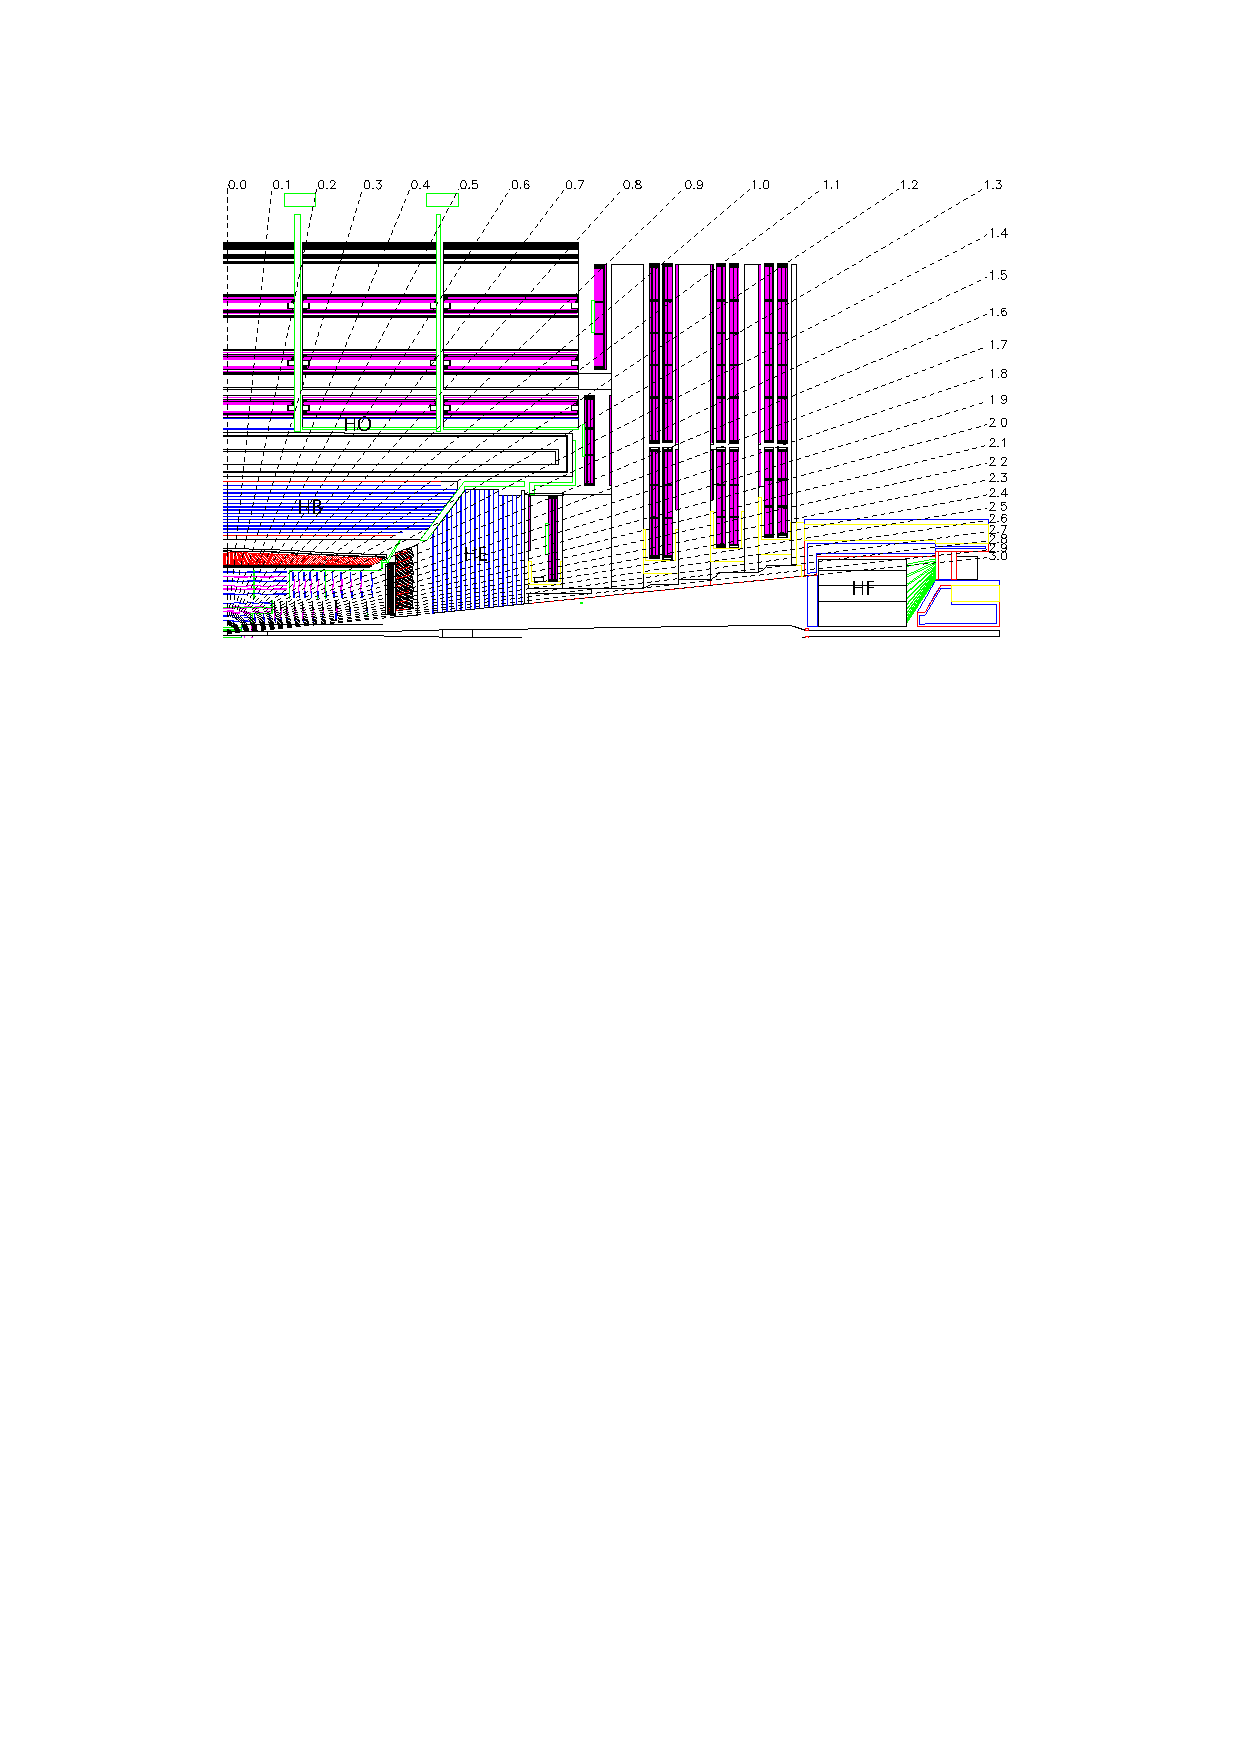
\includegraphics[width=\textwidth]{Chapters/02_Detector/Images/HCAL.pdf}\hfill
     \caption[A longitudinal schematic of the CMS HCAL.]{A longitudinal schematic of the CMS HCAL showing the
     location of the hadron barrel (HB), endcap (HE), outer (HO) and forward (HF) calorimeters
     \cite{CMS_experiment}.}
     \label{fig:CMS_HCAL}
\end{figure} 

\subsection{Superconducting Magnet}
\label{ss:Magnet}
The magnet of the CMS detector is the largest and highest field strength superconducting solenoid constructed
for a physics experiment in terms of bending power for physics and total stored energy~\cite{CMS_experiment}.
It can produce a magnetic field up to 4~\tesla~ (a field strength of 3.8~\tesla~ is used in normal operation)
with a stored energy of 2.7~\giga\joule~\cite{CMS_TDR1}. The cold bore, cooled to 4.5~\kelvin~ using liquid
helium, has dimensions of 12.5\m length and 6\m diameter, and weighs
220~tonnes~\cite{Cryogenic_System_for_Superconducting_Solenoid}.
Due to design constraints and structural requirements, the magnet itself provides some of the structural
strength both to support itself and to withstand its own magnetic bursting force on the coil
\cite{CMS_experiment}.

\begin{figure}[hbtp]
   \centering
     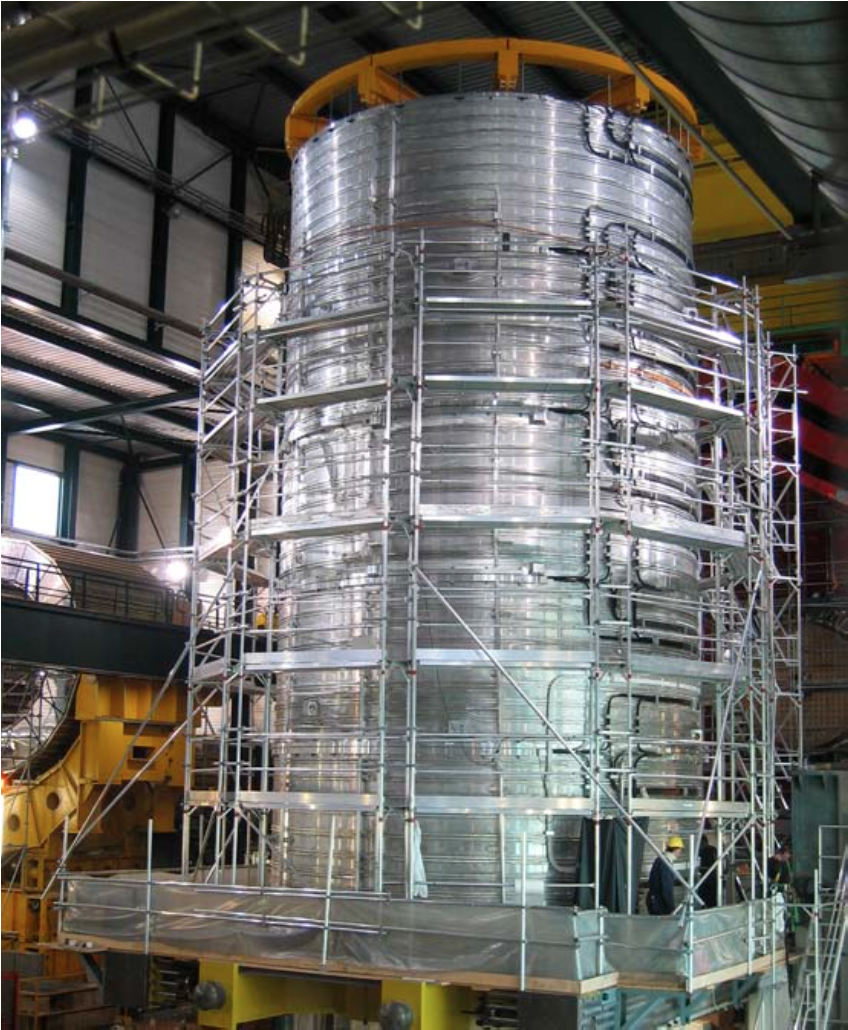
\includegraphics[width=0.5\textwidth]{Chapters/02_Detector/Images/Cold_mass.png}\hfill
     \caption[Bore of the CMS solenoid magnet in vertical position in the CMS assembly hall, SX5.]{Bore of the
     CMS solenoid magnet in vertical position in the CMS assembly hall, SX5, prior to installation \cite{CMS_experiment}}
     \label{fig:CMS_magnet_cold_bore}
\end{figure}
 
The cold bore, pictured in Figure~\ref{fig:CMS_magnet_cold_bore} in the CMS assembly hall, is enclosed in a
steel return yoke weighing 10,000~tonnes with the aim of containing and returning the magnetic field. The yoke
is interspersed with the muon chambers and is made up of 5 barrel segments and 6 endcap discs. The magnet was
designed in a manner such as to facilitate assembly at ground level prior to lowering into the CMS
experimental cavern, UX5. Despite the challenges involved in constructing such a powerful magnet, the high
bending-power created by the high magnetic field was desirable in order to provide good momentum
resolution of the tracking components.

\subsection{Muon Chambers}
\label{ss:Muon_Chambers}
Muons pass through all the previous inner sub-detectors, losing very little energy as they traverse them
(around 1\MeV/\mm on average), leading to the muon chambers being located outermost in the detector. There
are, in fact, three types of muon detectors in use in CMS. The endcaps contain Cathode Strip Chambers (CSCs),
the central barrel regions contain Drift Tubes (DTs), and both regions are equipped with Resistive Plate
Chambers (RPCs). These systems, in combination with the silicon tracker, are used to determine the momentum of
muons by taking advantage of their curved tracks due to the magnetic field. The different technologies are
used due to the different numbers of particles expected in different areas of the detector and because of
technological considerations regarding the physical areas to be covered~\cite{CMS_TDR1}.
Figure~\ref{fig:CMS_muon_system} shows a diagrammatic representation of one quarter of the CMS muon detectors.
The CSCs are used in the endcaps to cover \abseta values between 1.2 and 2.4 that experience high muon rates
and where the magnetic field of the solenoid is high~\cite{CMS_TDR1}. They take the form of four disc layers
each made of 2 (inner layer) or 3 (outer three layers) concentric rings. They consist of volumes of gas in
which positive wires placed at right angles to negative copper strips. To relate these to the name given to
these detectors, the positive wires are the anodes and the negative strips are the cathodes. As a charged
particle passes through the gas it ionises gas atoms and the electrons that are knocked out travel towards the
anode wires. At the same time the resulting positively charged ions in the gas travel towards the cathode
strips. Since the wires and strips are at right angles to each other, the CSCs provide two position
co-ordinates for the passing muon. The CSC detection mechanism is a fast process so their signals are used for
muon triggering \cite{CMS_experiment}.
 
\begin{figure}[hbtp]
   \centering
     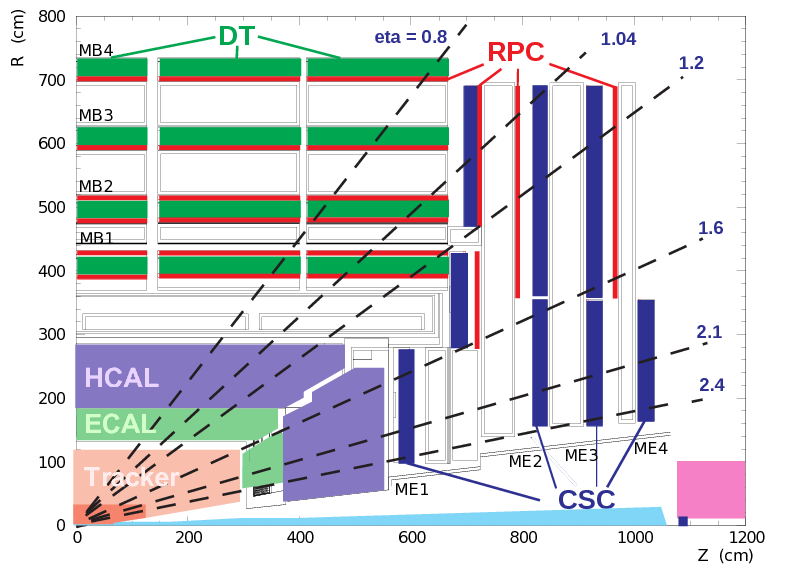
\includegraphics[width=0.65\textwidth]{Chapters/02_Detector/Images/MuonSys-mod3.png}\hfill
     \caption[Schematic representation of a quarter of the CMS muon system.]{Schematic representation of a
     quarter of the CMS muon system \cite{Muon_tracking}}
     \label{fig:CMS_muon_system}
\end{figure}

The barrel region DTs cover \abseta values of less than 1.2, that encounter low rates of low transverse
momentum muons~\cite{CMS_TDR1}. The drift tube chambers are arranged in four cylindrical layers, or stations,
among the layers of the magnet's iron return yoke and RPC layers. The stations are slightly staggered to
ensure that even a muon of high transverse momentum will be detected by at least three of the four layers. The
drift tubes contain a mixture of argon (85~\%) and carbon dioxide (15~\%), and a postively charged stretched
wire. As a particle with a charge traverses the volume of gas, atoms in the gas are ionised and the resulting
free electrons travel along electric field lines towards the positive wire. By using the position of the
electron along the wire and the time taken for the wire to detect the electron, two coordinates of the muon
position can be deduced.
In comparison to the DTs and CSCs, the RPCs that complement them provide a better resolution in terms of time
(1\ns) but a worse resolution in terms of position, and so provide additional trigger information. As their
name suggests, they are constructed of plates, one negatively charged (cathode) and one positively charged
(anode) and made of a plastic with high resistance. In a similar process to the other muon detectors, a gas
that makes up the volume in between the plates is ionised by a passing charged muon. The resulting electrons
create an avalanche of electrons by, in turn, ionising other gas atoms; this avalanche of electrons moves
towards the anode and metal readout strips outside the plastic anode detect the signal for readout. The hit
strips pattern allows a calculation of the muon momentum which is then fed to trigger algorithms.

\subsection{Trigger and Data Acquisition}
\label{ss:Trigger}
At the design bunch crossing frequency of 40~\MHz~ and at the design luminosity of $10^{34}\cm^{-2}\s^{-1}$,
the expected number of proton-proton collisions per second is approximately $10^{9}$, translating to 21
proton-proton collisions per bunch crossing on average. Each bunch crossing produces approximately 1~MB of
data, leading to 40,000\GB/\s~ of data. This extremely large amount of data, which is impractical to record,
means that a trigger system is required to filter the events in order to record only data that are of interest
for physics analyses.

There are two levels to the CMS trigger, named Level 1 Trigger (L1) and High Level Trigger (HLT). These work
with the electronics and readout systems in place in the detector to filter the events to a practically
manageable amount for processing. In combination, these triggers reduce the data rate by at least a factor of
$10^{6}$~\cite{CMS_experiment}.

The L1 Trigger is a pipelined deadtimeless system comprised of calorimeter triggers, muon triggers and a
global trigger that works on a combination of data from the former two. The decisions made by the L1 Trigger
are carried out by custom-designed hardware processors, consisting mostly of programmable electronics such
as Field Programmable Gate Arrays (FPGAs)~\cite{1742-6596-219-3-032009}. The data from a bunch crossing are held in
pipeline buffers in the electronics on the detector (at the front) end whilst the information for the triggers
is processed in the CMS service cavern (USC) and the decisions transmitted back to the front end. The maximum
time allowed for this process for each event is 3.2\us, which is the time taken for the signals to be
transmitted via optical fibres from the detector to the processors, processing time, and transmitted back
again. This time is known as the latency~\cite{CMS_TDR1}. The L1 Trigger outputs events to the HLT at a rate
of 100~\kHz~\cite{CMS_experiment}.

As mentioned, the trigger uses calorimeter and muon chamber data to reach a decision on an event
within the required timeframe. Tracker data are not currently used since track reconstruction exceeds the
amount of time allowed for the L1 trigger decision. Good trigger performance is related to the quality of the
calorimeters and muon systems. Factors such as good momentum resolution of high momentum muons, good charge
determination of muons, good ECAL energy resolution and good missing transverse energy resolution are required
for the trigger to select interesting events. The trigger was designed as described in order to allow the CMS
experiment to meet the goals of the LHC physics programme~\cite{CMS_experiment}.

Unlike the Level 1 Trigger, the High Level Trigger (HLT) is software-based and runs offline in HLT processor
farms of about a thousand commerical processors~\cite{CMS_TDR1}. If the Level 1 produces an accept decision,
the data which was stored in buffers in the front end electronics is read into readout buffers from where the
DAQ system accesses it. The L1 output rate of 100~\kHz~ corresponds to a data rate of approximately 100\GB/\s.
The HLT software processes these events in a computer farm that carries out fast processing of offline
algorithms such as selections and object reconstructions to reduce the rate down to approximately 100~\Hz.
These accepted data are then stored on tape. The HLT algorithms are designed based on the principle of
minimising the number of objects that need to be reconstructed in order to come to a decision, and events are
discarded as early as possible, leading to the HLT consisting of many virtual levels that progressively use
more information from, first, the muon chambers and calorimeters, followed by pixel tracker data, and finally
full tracker information~\cite{CMS_TDR1}.

Figure~\ref{fig:single_muon_trigger_rates} shows the variation in trigger rates with increasing muon
transverse momentum at luminosities of $2\times10^{33}\cm^{-2}\s^{-1}$ and $10^{34}\cm^{-2}\s^{-1}$. The rates
for different trigger levels are shown. The L1 trigger rate begins to flatten out as the \pt threshold
increases because the lack of tracker information at L1 means that low momentum muons mis-measured as having
high momentum are not removed. Thus, increasing the threshold would have no discernible effect on reducing the
trigger rates while reducing physics performance by rejecting desirable events. In comparison, the L3 trigger
rate, which includes tracker information, continues to decrease at high muon momenta, and is able to maintain
the rate at the desired level.
% Tracker data could thus be used for improved muon momentum resolution, in addition to electron matching, for
% the application of more efficient isolation criteria, and for primary vertex identification at the L1
% stage~\cite{Klein:1628930}.
% Incorporating the tracker information in the L1 trigger at the HL-LHC would therefore be an effective method
% of maintaining the L1 trigger rate at 100kHz at higher luminosities.

\begin{figure}[hbtp]
   \centering
     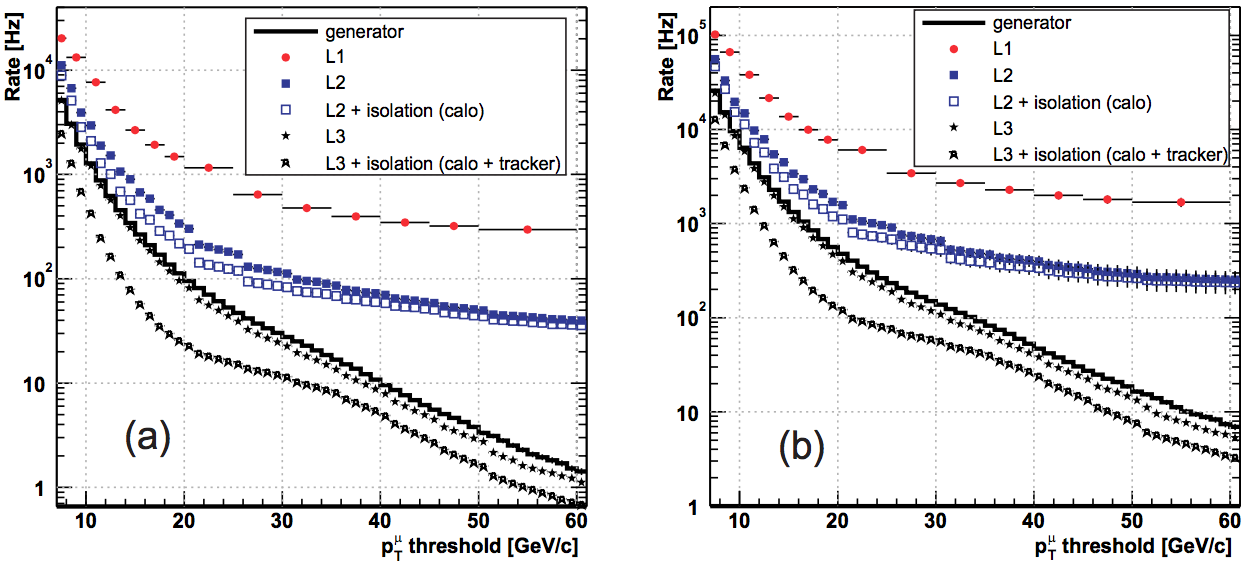
\includegraphics[width=0.65\textwidth]{Chapters/02_Detector/Images/Muon_trigger_rates.png}\hfill
     \caption[Single muon HLT rates at low and high luminosities.]{Single
     muon high level trigger rates at (a) $\mathcal{L}=2\times10^{33}\cm^{-2}\s^{-1}$ and (b)
     $\mathcal{L}=10^{34}\cm^{-2}\s^{-1}$~\cite{Cittolin:578006}.}
     \label{fig:single_muon_trigger_rates}
\end{figure}

A more detailed description of the data acquisition (DAQ) system can be found in \cite{CMS_experiment}
and \cite{CMS_TDR1}.

\section{Upgrades}
\label{s:Upgrades}
The CMS experiment, along with the LHC and the other detectors are in a long term programme of upgrades and
maintenance. By 2023 the luminosity provided by the LHC is expected to be $2\times10^{34}\cm^{-2}\s^{-1}$
\cite{Technical_Proposal_Upgrade_of_CMS_Detector_through_2020}. The various runs and shutdowns until 2023 are
collectively referred to as Phase 1. In phase 2, or after 2023, long shutdown 3 is also planned to bring
further improvements and upgrades to the performance of the LHC, after which the luminosity of the LHC is
expected to reach $5\times10^{34}\cm^{-2}\s^{-1}$. The machine in this state will be known as the high
luminosity LHC, HL-LHC (also sometimes referred to as Super LHC, SLHC).

Naturally, the above dates and schedules are the latest best estimates and are liable to change over time,
particularly those further in the future, as work progresses.
\chapter{CMS Computing and Offline}
\label{c:CMS_computing_and_offline}

\section{CMS Computing}
\label{s:CMS_computing}

The CMS offline computing infrastructure takes on the workload of transferring accepted data from the triggers
to both permanent and temporary storage, of processing this data for subsequent analysis, in addition to the
production of simulated CMS data. The resources needed to process the high volumes of data involved require a
distributed computing system. The Worldwide LHC Computing Grid (WLCG) infrastructure, an international
collaboration of LHC experiments and computing centres, is employed to carry out these tasks.

CMS computing resources are primarily divided into three tiers. Tier 0 (T0) consists of only one site, at CERN
itself. The T0 centre has as its main aim to take accepted data from the detector and transfer it to permanent
storage on tape. Tier 0 computing is also responsible for reconstructing the initial RAW data into smaller
formats, by passing events through modules to produce physics objects (like electrons and jets) using
algorithms to reconstruct tracks in the silicon tracker, clusters of deposits in the calorimeters, primary and
secondary vertices, determine particle identification and to correct for detector characteristics such as
non-functioning components (see Section~\ref{s:Event_Data_Model} onwards for more details on data formats).
From the T0 centre, copies of the data in RECO and RAW format are transferred to T1 centres around the world.
Owing to its crucial role in ensuring the reliable transfer of RAW and RECO data, T0 resources are not
available for analysis by CMS users. There are seven Tier 1 centres located in various countries within the
CMS collaboration. The UK T1 centre is located at the Rutherford Appleton Laboratory in Harwell, near Oxford.
T1 centres provide reliable computing resources for data storage and processing. RAW data is spread between
them, providing a second copy of the RAW data stored at CERN. The second reconstruction step, termed RERECO,
is also carried out at T1 centres, in addition to the production of simulated data. These can then be provided
to any of the Tier 2 centres at CMS institutes (typically universities) where they may be temporarily stored.
T2 centres are also generally used to run users' final analyses and produce simulations
\cite{CMS_experiment,CMS_TDR1}.

\section{Event Data Model}
\label{s:Event_Data_Model}
Reconstructed data from CMS uses a data model based around an event, called the Event Data Model (EDM), where
one event is one crossing of proton bunches at the centre of CMS that passes the triggers. This model
is created and manipulated within a CMS software framework (CMSSW)~\cite{cmssw} written in C++, with the event
and related objects in the object-oriented data analysis framework ROOT~\cite{ROOT}.

The iterations of data from the initial recorded information to subsequent, more compact formats, are produced
by passing events through a sequence of modules. The arrangement of these data takes the form of several
layers, with the first of these being RAW. This level contains the full information from the event in CMS and
occupies approximately 1.5-2~MB/event. More information than is necessary for user analyses is included at
this level, and so the majority of CMS users will not use this data format. Reconstructed level data (RECO) is
slightly smaller in size (approximately 0.5~MB/event) and is essentially a compressed subset of the RAW data
after modules performing reconstruction have been run.

The third level, Analysis Object Data (AOD), is the smallest of the data formats, requiring approximately
100~kB/event, which is small enough to allow the entire AOD data to be stored at computing centres worldwide.
AOD format is a subset of the RECO data, and is produced by further reducing RECO, leaving only high level
physics objects (e.g. electrons, jets) which is adequate for most physics analyses. 

In the differential cross section analysis presented in this thesis, this AOD data is processed using the
Bristol Top Group's NTupleProduction code~\cite{NTT_LukeKreczko_SergeySenkin_JesonJacob_EmyrClement_2015} to
produce private ntuples which are yet again smaller in size, at approximately 3~kB/event. These ntuples are
then converted to simple ROOT histogram files after applying the required selection criteria and corrections
in the BristolAnalysisTools~\cite{BAT_LukeKreczko_JesonJacob_SergeySenkin_EmyrClement_2015}. Scripts written
in Python in DailyPythonScripts~\cite{DPS_LukeKreczko_SergeySenkin_JesonJacob_EmyrClement_2015} are then used
to produce final results plots and tables.


\section{Object Reconstruction and Identification}
\label{s:object_reconstruction_and_identification}

The process of producing a physics object such as an electron, photon or jet, from the data recorded by CMS is
known as reconstruction and is carried out by modules qknown as EDProducers within CMSSW. The three-step
process of reconstructing high level objects consists of local reconstruction within a sub detector, global
reconstruction using data from the whole CMS detector, and a final stage combining reconstructed objects from
the first two stages. The reconstruction technique used in the majority of CMS analyses is called Particle
Flow (PF) \cite{particle_flow}. PF uses information from all of the sub-detectors of CMS to identify and reconstruct
particles produced from a proton-proton collision.

\subsection{Track Reconstruction}
\label{ss:track_reconstruction}
Algorithms performing local track reconstruction execute a scan to identify tracker modules that receive a
higher than threshold signal. Clusters are then constructed by adding adjacent strips or pixels to the
originally identified seed strip or pixel. In order to reconstruct complete tracks to obtain the position and
momentum of the charged particle, algorithms based on specific requirements such as high or low transverse
momentum tracks are used. These algorithms in CMS are collectively known as the Combinatorial Track Finder
(CTF).

Multiple passes of the CTF reconstruction software are carried out to reconstruct tracks, in a process called
iterative tracking. The earliest iterations identify tracks that are easy to find such as high \pt tracks
originating near the interaction point. As these tracks are reconstructed, the corresponding hits are removed
from consideration in subsequent iterations, making it simpler for later iterations to identify tracks that
are more difficult to find such as those of displaced particles or with low \pt.

Six iterations are carried out in total, and each iteration can be split into four steps. Seeds are created
using 2 or 3 hits to produce intial track candidates. The seed gives an estimate of the trajectories of the
potential track candidates. A Kalman Filter \cite{kalman_filter, Speer:927395} based track finding algorithm
then looks for further hits along an extrapolated path of the seed trajectory. A track fitter is then run
using information from the previous steps to produce final values for trajectory parameters. The fourth and
final step then rejects tracks which fail specified quality checks \cite{track_reconstruction}.

\subsection{Pileup Subtraction}
\label{ss:pileup_subtraction}
When reconstructing an event in CMS, all vertices (points from which multiple tracks originate) in the event
must be reconstructed. By ordering the vertices by the sum of the transverse momenta of their tracks, it is
possible to identify the the vertex of interest for physics analyses, known as the primary vertex (PV), as the
vertex with the largest transverse momentum. The particle flow algorithm reconstructs objects, starting with
those coming from the primary vertex, followed by other vertices (known as pileup). The reconstructed objects
from the PV can be affected by the number of other vertices present in the event. For example, the jet
momentum and lepton isolation could both increase with high pileup. This can, in turn, lead to signal events
not passing selection requirements because a truly isolated lepton from the PV may appear not to be isolated.
In addition, a larger number of events from background processes may pass selection requirements due to low
energy jets appearing to have a higher energy. Hence, pileup subtraction, the removal of charged particles
coming from vertices other than the PV is implemented to reduce these effects.

Neutral particles, however, pose a more difficult problem since they leave no tracker information for the
reconstruction algorithms to easily identify their origin. One method of removing such particles from an
event, known as the $\Delta\beta$ correction, uses the fact that the estimated average energy in an event from
neutral particles is half that from charged particles. Thus, it can be estimated that 0.5 times the charged
particle energy comes from neutral particles. The second method, known as $\rho$ correction, subtracts an
average transverse momentum coming from pileup per unit area. While the two methods produce similar results,
the $\rho$ correction is used to correct the electron isolation and the $\Delta\beta$ correction is used to
correct the muon isolation in the differential cross sections analysis presented in this thesis, as
recommended by the CMS TOP physics analysis group.

\subsection{Electron Reconstruction}
\label{ss:electron_reconstruction}
ECAL local reconstruction algorithms calculate the time of arrival, position and the energy of deposits. After
grouping together deposits in neighbouring crystals to form clusters, deposits are then matched to deposits in
the HCAL, forming a Calo Tower. Electrons are, typically, completely stopped in the ECAL and deposit their
energy in a narrow cluster of crystals.

However, electrons can interact with the material between the interaction point and the ECAL, emitting a
photon via bremsstrahlung radation. Similarly, photons can convert to an elecron-positron pair ($e^{+}e^{-}$).
Both of these processes result in ECAL deposits with a larger spread in $\phi$ because of the strong magnetic
field in the inner section of CMS containing the tracker. In the case of photons, several clusters are grouped
together to form superclusters, which are then corrected for their energies to obtain the energies of the
original photon \cite{photon_reconstruction}.

Electron reconstruction in the ECAL is carried out by two methods. The first matches superclusters with a
trajectory compatible with two or three pixel detector hits and the interaction point. The second matches the
supercluster to tracker tracks to identify electrons (and in the case of electrons emitting bremsstrahlung
radiation, tracks with a low number of hits) \cite{electron_reconstruction}. Combining the seeds from the two
methods, a Gaussian-Sum Filter, a generalisation of the Kalman Filter algorithm, is used to reconstruct
electron paths \cite{electrons_GSF}.

Since other objects can leave similar signatures in the detector to electrons, such as jets or electrons from
photon conversions, candidates are required to satisfy additional requirements of identification and
isolation. Several electron identification methods exist and are used in CMS analyses. The top cross sections
analysis in this thesis uses the multivariate identification (MVA ID). As the name suggests, this approach
uses a multivariate analysis, with track, track quality, and supercluster variables as input, to produce a
discriminator value, with higher values indicating a higher likelihood for a candidate to be a real electron.
The MVA ID algorithm is optimised for identifying electrons from W and Z boson decays, and separately for
triggering and non-triggering electrons~\cite{electron_reconstruction}.

The isolation of an electron is defined as the activity within a cone surrounding the electron. Isolation is
used as an additional criterion to select electrons, in particular to distinguish electrons promptly produced
in a proton-proton collision. Such isolated electrons would have less activity in its vicinity than electrons
from within a jet, which could originate from leptonically decaying b hadrons, and jets faking electrons. Two
methods exist in CMS of calculating the isolation of a particle: detector based isolation and particle based
isolation. The detector based method is defined in each sub detector as the sum of the momenta or energies in
a cone of $\Delta R = 0.3$ around the electron. The particle based method uses the total transverse energy of
PF reconstructed particles within a cone of $\Delta R = 0.3$ and can remove activity coming from collisions
other than the hard proton-proton interaction of interest. By normalising this isolation to the momentum or
energy of the electron, a relative isolation is obtained, relating the cone activity to the electron.
Termed PFRelIso, it is this relative isolation that is used in the cross section analysis to select
electrons.
% can improve signal efficiency

In order to avoid the selection of electrons originating from a photon conversion, a veto can be placed on a
second electron in the event. However, since the two electrons in a photon conversion may not necessarily have
equal transverse momentum, \ie one may have a very low \pt, such a veto may be insufficient, and so further
techniques to identify conversion events are used. Firstly, since an electron from a conversion would be
produced at some distance from the interaction point and in the detector material, eliminating candidates with
missings hits in the pixel tracker helps to distinguish such electrons from promptly produced electrons. In
events in which the conversion occurs in the beam pipe or if the electron is matched to unassociated pixel
hits, this method can also be insufficient, so an additional track matching step is used. Tracks are matched
in pairs and following geometrical cuts, can be removed if they appear to originate from a conversion
\cite{electron_reconstruction}.

\subsection{Muon Reconstruction}
\label{ss:muon_reconstruction}
Local reconstruction in the muon chambers provides hit position and time of arrival of a muon. This
information from the DTs and CSCs is then amalgamated to create muon track hits and segments, which are then
used by the muon global reconstruction algorithms to reconstruct ``standalone'' muons. An inner detector
segment is used as a seed for a Kalman Filter~\cite{kalman_filter, Speer:927395} and possible trajectories are
generated. By removing hits which are unlikely to have come from the track in question, the likely trajectory
is constructed layer-by-layer. A final fit is carried out, including an extrapolation to the interaction point
for greater momentum resolution.

Muons are also independently reconstructed in the tracker. These tracker tracks can therefore be combined with
the aforementioned muon chamber information, where the magnetic field is only 2~\tesla, to improve the \pt
resolution of muons, as seen in Figure~\ref{fig:muon_momentum_resolution}.

\begin{figure}[hbtp]
   \centering
     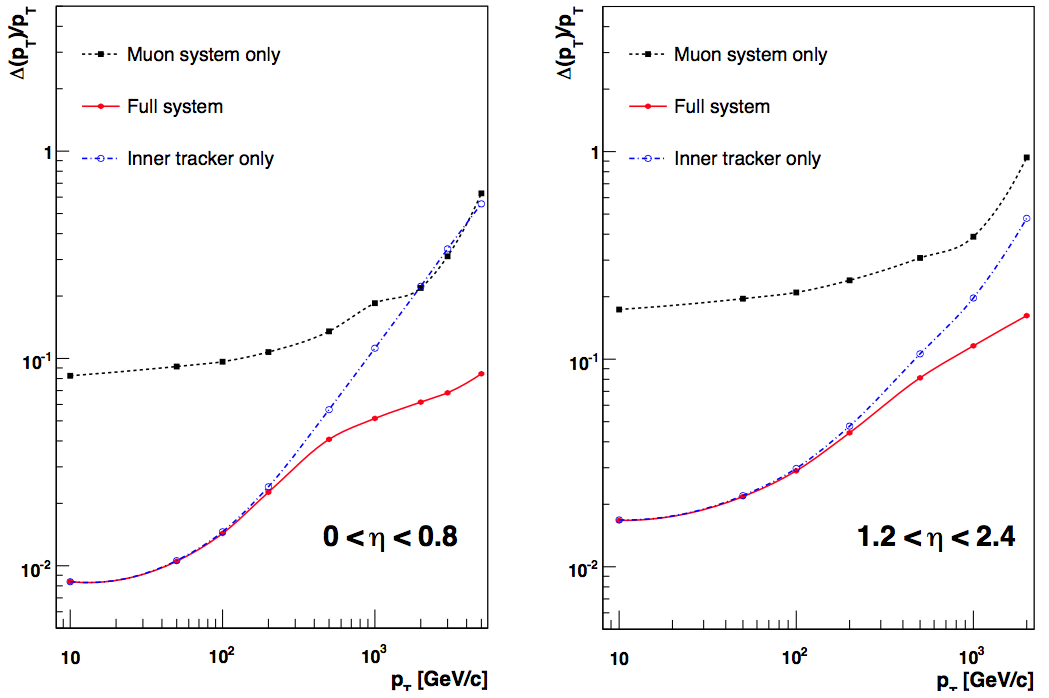
\includegraphics[width=0.65\textwidth]{Chapters/02_Detector/Images/muon_momentum_resolution.png}\hfill
     \caption[Muon transverse momentum resolution using muon system and the tracking system.]{Muon transverse
     momentum resolution as a function of muon transverse momentum using the muon system only, using inner tracking only,
     and using both~\cite{Chatrchyan:2012xdj}.}
     \label{fig:muon_momentum_resolution}
\end{figure}

Two methods are employed to combine the information from the two sub-detectors. \textit{Global muon
reconstruction} matches a tracker track to a standalone muon track and carries out a fit of the resulting
\textit{global muon} track. The second method, \textit{tracker muon reconstruction}, extrapolates tracker
tracks outwards to the muon chambers and accepts a muon candidate if a DT or CSC matching track is found and
the muon \pt is greater than 0.5\GeV~\cite{muon_reconstruction}.

For triggering, the \pt of a muon is first estimated using the information available at Level 1 from all three
types of muon detectors. At HLT level, the muon candidates from Level 1 are further refined using track
finding and fitting, but still using only information from muon chambers, leading to Level 2 muons. As
mentioned in Section~\ref{ss:Trigger}, due to the time constraints required of the L1 trigger, full tracker
data are not currently used. However, tracks of Level 2 muons are extrapolated into the tracker systems and a
localised track finding algorithm is run to identify only nearby tracker hits. A track matching that of a
Level 2 muon leads to a Level 3 muon. %See Emyr's thesis P45 top for details.

\subsection{Jet Reconstruction}
\label{ss:jet_reconstruction}
As quarks produced in proton-proton interactions (except the top quark) hadronise~\cite{Griffiths:1987tj},
jets of particles are formed in the direction of travel of the quark. The time of arrival, position and the
energy deposited by hadronic objects are locally reconstructed in the HCAL. If the deposit matches an ECAL
deposit, a Calo Tower is formed for later use in jet reconstruction algorithms.

The PF algorithm performs the reconstruction of particles in the jet, and the \antikt algorithm is used to
perform the clustering of these particles into jets. The \antikt algorithm, explained in detail
in~\cite{Cacciari:2008gp}, is one of several jet algorithms that exist in CMS to combine reconstructed
particles into jets. It defines a distance $d_{ij}$ between reconstructed particles as
\begin{equation}
%\begin{center}
d_{ij} =
min\left(\frac{1}{p_{T,i}^{2}},\frac{1}{p_{T,j}^{2}}\right)\frac{(\eta_{i}-\eta_{j})+(\phi_{i}-\phi_{j})^{2}}{R^{2}}.
%\end{center}
\end{equation}
$p_{T,i}$ and $p_{T,j}$ are the transverse momenta of the two particles $i$ and $j$, $\eta_{i}$ and $\eta_{j}$
are the rapidities, $\phi_{i}$ and $\phi_{j}$ are the azimuth angles and $R$ is the radius of the jet cone.
The \antikt algorithm iteratively clusters together particles with the smallest $d_{i,j}$ between them until
all jets are reconstructed and there are no particles remaining. Events will usually consist of a small number of
high-\pt (hard) particles and a large number of low-\pt (soft) particles. The distance between hard particles
is typically small, and the distance between softer particles is larger. Soft particles tend to
cluster around hard particles first, before clustering with other soft particles.

While the PF anti-$k_{t}$ jets show high jet matching efficiency on Monte Carlo simulation samples,
corrections are applied based on the jet $\pt$ and $\eta$ to correct for mismeasurements in the
detector and thereby improve the agreement between generated and reconstructed particle flow jets. The
factored approach to CMS jet energy corrections is comprised of three parts:
\begin{enumerate}
  \item {L1 Pile Up: corrects for additional energy from charged particles from pile-up in the event
  \ref{ss:pileup_subtraction}.}
  \item {L2 Relative Jet Correction: corrects the reconstructed energy to match the generated jet with respect
  to $\eta$.} %to flatten the jet response in the ecal eta
  \item {L3 Absolute Jet Correction: corrects the reconstructed energy to match the generated jet with respect
  to $\pt$.} %to flatten the jet response in the ecal pt
  \item {L2L3Residuals: reduces any residual differences between the reconstructed and generated
  jet due to simulation not being perfectly tuned to data. This correction is applied to data only.}
  %https://twiki.cern.ch/twiki/bin/viewauth/CMS/IntroToJEC
\end{enumerate}
In order to identify jets in the differential cross sections analysis, further identification criteria are
used to reduce electronic noise, to reduce the number of electrons mis-identified as jets and, in so doing, to
ensure the selection of high quality jets. The requirements, which are known as the loose PF Jet ID, are:

\begin{itemize}
  \item at least one constituent particle
  \item the neutral hadron energy fraction (NHF) must be $<0.99$
  \item for jets with \abseta$<2.4$, the charged hadron energy fraction (CHF) must be $>0$
  \item the neutral electronmagnetic energy fraction (NEF) must be $<0.99$
  \item for jets with \abseta$<2.4$, the charged electronmagnetic energy faction (CEF) must be $<0.99$
  \item for jets with \abseta$<2.4$, the number of charged hadronic constituents (NCH) must be $>0$
\end{itemize}

\subsubsection{B Jets}
\label{sss:b_jets}
The process of identifying jets coming from \bquarks is known as \btagging and is very important in top quark
physics due to the decay of the top to a \W boson and a \bquark. Effective \btagging can therefore help to
appreciably reduce background processes in an analysis. A description of \btagging, the several algorithms
available in CMS, relevant event variables, and a performance comparison, is given in
Chapter~\ref{c:b_tagging_study}.

\chapter{The Standard Model of Particle Physics}
\label{c:the_standard_model}

\section{Introduction}
\label{s:standard_model_intro}

The Standard Model (SM) is the name given to the theory developed during the course of the \nth{20} century
that describes the elementary particles that make up all known, observable matter and the three fundamental
forces by which they interact (electromagnetic, weak and strong). The SM does not, however, describe the
gravitational force as it is not known how to model it mathematically at a quantum scale. The SM puts forward
twelve fermions, with a spin quantum number of 1/2, as the matter particles. These are split into two groups
of six quarks and six leptons, all of which are split into three generations. The six quarks are classified
according to their charge and flavour: up, down, charm, strange, top and beauty quarks. The leptons are in
turn classified according to their charge and flavour: electron, muon or tau leptons, together with their
corresponding neutrinos. Neutrinos, although originally thought to be massless, are now believed to carry mass
due to the observation of the oscillation of neutrinos between different flavours.
Table~\ref{tab:standard_model} shows these particles of the Standard Model in their respective generations.
All of these particles have a respective antiparticle which has identical quantum numbers except opposite
electric charge.

\begin{table}[hbth]
\centering
\begin{tabular}{lllll}
\hline
Generation & Flavour & Charge / $e$ & Spin & Mass /\MeV \\
\hline
\hline
\multicolumn{5}{c}{\textbf{Leptons}} \\
\hline
\multirow{2}{*}{I} & electron (e) & -1 & $\frac{1}{2}$ & 0.511 \\
 & electron neutrino ($\nu_{e}$) & 0  & $\frac{1}{2}$ & 0 \\
\hline
\multirow{2}{*}{II} & muon ($\mu$) & -1 & $\frac{1}{2}$ & 105.66 \\
 & muon neutrino ($\nu_{\mu}$) & 0 & $\frac{1}{2}$ & 0 \\
\hline
\multirow{2}{*}{III} & tau ($\tau$) & -1 & $\frac{1}{2}$ & 105.66 \\
 & tau neutrino ($\nu_{\tau}$) & 0 & $\frac{1}{2}$ & 0 \\
\hline
\hline
\multicolumn{5}{c}{\textbf{Quarks}} \\
\hline
\multirow{2}{*}{I} & up (u) & $+\frac{2}{3}$ & $\frac{1}{2}$ & $2.3^{+0.7}_{-0.5}$ \\
 & down (d) & $-\frac{1}{3}$ & $\frac{1}{2}$ & $4.8^{0.5}_{-0.3}$ \\
\hline
\multirow{2}{*}{II} & charm (c) & $+\frac{2}{3}$ & $\frac{1}{2}$ & $(1.275^{+0.025}_{-0.025}) \times 10^{3}$ \\
 & strange (s) & $-\frac{1}{3}$ & $\frac{1}{2}$ & $95^{+5}_{-5}$ \\
\hline
\multirow{2}{*}{III} & top/truth (t) & $+\frac{2}{3}$ & $\frac{1}{2}$ & $(173.21\pm{0.51}\pm{0.71}) \times 10^{3}$ \\
 & bottom/beauty (b) & $-\frac{1}{3}$ & $\frac{1}{2}$ & $(4.18^{+0.03}_{-0.03}) \times 10^{3}$ \\
\hline
\hline
\multicolumn{5}{c}{\textbf{Bosons}} \\
\hline
Force & Gauge Boson(s) & Charge / $e$ & Spin & Mass /\GeV \\
\hline
Weak & $\W^{+} / \W^{-} / \Z^{0}$ & +/-/0 & 1 & $80.385\pm0.015 / 91.188\pm0.002$ \\
Electromagnetic & photon ($\gamma$) & 0 & 1 & 0 \\
Strong & gluon (g) & 0 & 1 & 0 \\
Gravitation & graviton & 0 & 1 & 0 \\
- & Higgs (H) & 0 & 0 & $125.7\pm0.4$ \\
\hline
\end{tabular}
\caption{Fundamental fermions, split into their three generations, and bosons of the Standard Model.
Particle properties taken from \cite{Agashe:2014kda}.}
\label{tab:standard_model}
\end{table}



All known, observable matter in the universe is composed of the aforementioned twelve fermions or their
antiparticles. All stable matter is composed of protons, neutrons and electrons. All other particles are
unstable and decay; they are produced only in particle colliders such as the LHC, or in cosmic radiation.
Quarks also carry the charge of the strong force, termed `colour', of red, green or blue. The only quark which
does not hadronise (form bound colourless states) is the top quark which has a very short lifetime of
$\approx5\times10^{-25}\s$~\cite{Agashe:2014kda} due to its large mass, and therefore decays before it can
hadronise.

These fermions interact via the integer spin (spin 1) gauge bosons of the three fundamental forces. Electron,
muon and tau leptons interact via the electromagnetic and weak forces; their neutrinos, since they carry no
electric charge, interact only via the weak force; and the quarks interact via the electromagnetic, weak and
strong forces. Each of the forces are mediated by gauge bosons that are the `force carriers', and lead to the
formation of hadrons and atoms. The mediator of the strong force is known as the gluon, that of the
electromagnetic force is the photon and those of the weak force are the $\W^{+}$, $\W^{-}$ and $\Z$ bosons.
Table~\ref{tab:standard_model} shows the gauge bosons and their properties.

% The range of action of the boson determines the interaction range of the force it carries. Heavier bosons,
% like the $\W^{+}$, $\W^{-}$ and $\Z$ bosons, have a short range of action, while massless bosons such as
% photons and gluons have a theoretically infinite range. In reality, this is not the case because the gluons
% themselves carry the strong colour charge and so interact with each other, reducing their interaction range.
The strength of the fundamental forces is quantified by their coupling strength, denoted $\alpha$. Taking the
strength of the strong force as the baseline, the relative strength of the electromagnetic force is $10^{-2}$,
that of the weak force is $10^{-5}$ and the strength of the gravitational force is
$10^{-39}$~\cite{Rolnick_Fundamental_Particles}. The electromagnetic coupling strength, also known as the
fine-structure constant, is defined as $\alpha_{em}=\frac{e^{2}}{4\pi}$, which at low energies is
$\approx\frac{1}{137}$. Although the strong force is the strongest force, it has a limited range of only
\textasciitilde$~10^{-15}\m$, and the weak force has an estimated range of \textasciitilde$10^{-18}\m$, while
the electromagnetic and gravitational forces have infinite range.

The Higgs boson, the discovery of which was announced in July 2012 by the CMS and ATLAS experiments at the
LHC, is the latest component of the Standard Model to be discovered \cite{Chatrchyan:2012xdj, Aad:2012tfa}.
The mechanism of electroweak symmetry breaking through which other particles acquire mass is due to the Higgs
field, and is described in Section~\ref{ss:spontaneous_symmetry_breaking}.

\subsection{Gauge Principle}
\label{ss:gauge_principle}
The underlying mathematical model of the Standard Model is a Quantum Field Theory (QFT) combining special
relativity and quantum mechanics. All interactions in the SM must conserve the kinematic quantities energy and
momentum, in addition to electric charge. In addition, the electromagnetic and strong forces conserve the
dynamic quantities colour, baryon number, lepton number and quark flavour. The weak force, if mediated by a
charged propagator ($\W^{\pm}$), can allow the violation of quark flavour, meaning a quark can decay into
another flavour quark.

The laws of conservation occur as a result of underlying symmetries in the theories. For instance, energy
conservation stems from time symmetry and angular momentum conservation is a result of rotational symmetry.
In addition to these classical symmetries, a quantum field theory can also possess gauge symmetries. The
principle of gauge invariance refers to field theories in which the Lagrangian, which summarises the dynamics
of the system, is invariant under local transformations (transformations that are a function of a field, and
therefore different at all space-time points within the field). %The collection of all such transformations,
% called gauge transformations, are called the Lie group.
If the collection of all such gauge transformations, is commutative, \ie any order of application of the
symmetry transformations produces the same result, the theory is termed Abelian. Conversely, if the group is
non-commutative, the theory is non-Abelian. Each group of transformations has an associated generator, and
each generator has a corresponding vector field, or gauge field, whose purpose is ensuring invariance under
local transformations. The quanta of these fields are the gauge bosons of the Standard Model. Note that the
converse of local transformations are global transformations, in which the transformation takes place
instantaneously at all space-time points.
% However, the speed of any tranformation is limited to c, the speed of light, and so a more realistic local
% transformation is interesting to consider.

Group transformations can be represented as groups of $n \times n$ matrices which possess properties such as
unitarity ($U$) and orthogonality ($O$). A group of matrices with determinant 1 is called `special' ($S$),
leading to further groups $SU(N)$ and $SO(N)$. The Standard Model is comprised of electroweak theory
(combining electromagnetism and weak theory) a gauge group of $SU(2) \times U(1)$ and the theory of strong
interactions that has a gauge symmetry of $SU(3)$. The Standard Model is therefore a gauge theory based on the
gauge group $SU(3) \times SU(2) \times U(1)$.

\subsection{Quantum Electrodynamics}
\label{ss:quantum_electrodynamics}

Quantum electrodynamics (QED) is a component theory of the Standard Model that governs the interactions of
electrically charged particles. The simplest electromagnetic process is shown in
Figure~\ref{fig:qed_processes}a, and all real processes are made of some number of these processes combined
together, such as electron-positron annihilation shown in Figure~\ref{fig:qed_processes}b.

\begin{figure}[hbtp]
   \centering
     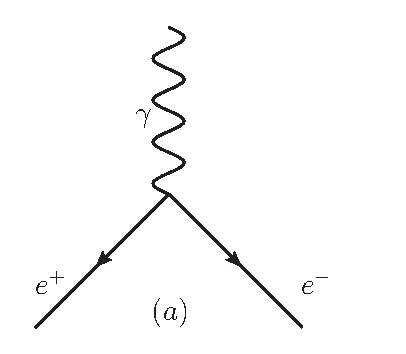
\includegraphics[width=0.3\textwidth]{Chapters/03_Theory/Images/e_e_gamma}\hfill
     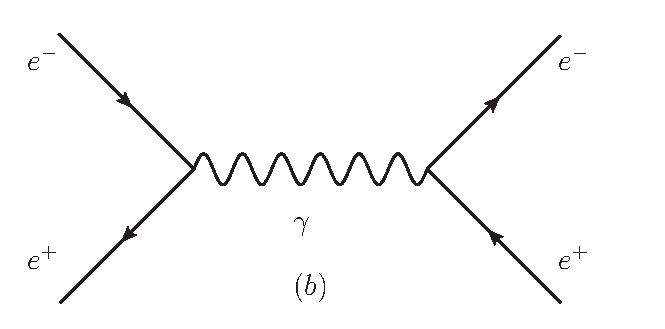
\includegraphics[width=0.5\textwidth]{Chapters/03_Theory/Images/e_e_gamma_e_e}
     \caption[Elementary electromagnetic processes.]{(a) the elementary electromagnetic process of an electron
     emitting a photon and (b) electron-positron annihilation.}
     \label{fig:qed_processes}
\end{figure}

Any such real process is represented by the sum of all possible orders of Feynmann diagrams for a possible
interaction is the representation of the real process. In practice, since at low energies, each vertex
contributes a factor of $\alpha$, higher-order Feynmann diagrams with more than a few vertices contribute
negligibly to the process and are often ignored.

The coupling strength of a force can be further explained in terms of vacuum polarisation. Regarding the
electromagnetic force, this refers to the phenomenon of electron-positron pairs and photons being
spontaneously created and absorbed by an electron. These virtual particles, which would be represented in
Feynmann diagrams as closed loops, shield the original electron leading to the electron charge being measured
at a lower value than its true charge. This measured value is called the effective, or 'screened', charge. As
a result, the coupling strength of the electromagnetic force is said to be a `running' coupling
constant, due to the fact that it decreases as a function of distance.

The mathematical formulation of QED stems from the Dirac equation, which describes the Lagrangian for a
spin-half (Fermionic) field $\psi$~\cite{Dirac610}:

\begin{equation}
\calL = i (\hbar c) \bar{\psi} \gamma^{\mu} \partial_{\mu} \psi - (mc^{2}) \bar{\psi} \psi
\end{equation}

Here, $\hbar$ is the reduced Planck's constant, $\mu$ are the Lorentz indices and $\gamma^{\mu}$ are the gamma
(or Dirac) matrices. Under a global transformation of the field by a phase $i \alpha$,
%\begin{equation}
%\psi(x) \rightarrow \psi'(x) = e^{i\alpha}\psi(x), \bar{\psi} \rightarrow \bar{\psi}'(x) =
%e^{-i\alpha}\bar{\psi}(x)
%\end{equation}
%
this Lagrangian is invariant (\ie under a global transformation of the $U(1)$ group, since this is
equivalent to multiplication of the field $\psi$ by a $1 \times 1$ unitary matrix). However, under a local
gauge transformation by a phase of $i\alpha(x)$, the symmetry %is no longer true since the partial derivative
no longer holds
%\begin{equation}
%\partial_{\mu}(e^{i\alpha(x)}\psi) = i(\partial_{\mu}\alpha(x))e^{i\alpha(x)}\psi +
%e^{i\alpha(x)}\partial_{\mu}\psi ,
%\end{equation}
%
meaning the Lagrangian is not invariant:
\begin{equation}
\calL \rightarrow \calL - \bar{\psi}(x)\gamma^{\mu}\psi(x)[\partial_{\mu}\alpha(x)].
\end{equation}

Local symmetry can be maintained in this case if a new gauge field, $A_\mu$, is introduced to the Lagrangian
by means of a covariant derivative $D_\mu$.%:
%\begin{equation}
%D_{\mu} = \partial_{\mu} + ieA_{\mu}.
%\end{equation}
%
%Under the local transformation, $A_{\mu}$ tranforms as
%
%\begin{equation}
%A_{\mu} \rightarrow A_{\mu}' = A_{\mu} - \frac{1}{e}\partial_{\mu}\alpha(x).
%\end{equation}
%
If the partial derivatives in the Dirac equation are now replaced with the covariant derivatives, the
invariant Lagrangian is obtained:
\begin{equation}
\calL = i (\hbar c) \bar{\psi} \gamma^{\mu} \partial_{\mu} \psi - e \bar{\psi} \gamma^{\mu} \psi A_{\mu} -
(mc^{2}) \bar{\psi} \psi - \frac{1}{4}F^{\mu\nu}F_{\mu\nu}.
\end{equation}

In this way, the principle of local gauge invariance under the $U(1)$ group is used to introduce additional
fields to a Lagrangian in order to make it invariant under local transformations. This final Lagrangian is
that of quantum electrodynamics. The physical interpretation of the gauge field $A_{\mu}$ is the photon, which
couples to charged particles (electrons and positrons) with a coupling strength proportional to the charge.
The term $\frac{1}{4}F^{\mu\nu}F_{\mu\nu}$ is an additional term to account for the kinetic energy of the free
particle of the new gauge field, \ie the photon; and there is no term giving the photon mass.

% \begin{equation}
% F_{\mu\nu} = \partial_{\mu}A_{\nu} - \partial_{\nu}A_{\mu}.
% \end{equation}

\subsection{Electroweak Theory}
\label{ss:electroweak_theory}

The unification of the electromagnetic and weak forces in the 1960s provided a more complete theory of
fundamental particles. This unification takes the form of an $SU(2) \times U(1)$ gauge group combining the
electromagnetic and weak forces, and can be constructed in a similar way to the QED formalism in
Section~\ref{ss:quantum_chromodynamics}.

First, it is necessary to define isospin, $I$, an abstract fundamental property of fundamental particles that
is conserved in all interactions. Similarly, weak hypercharge, $Y$, is also a quantum property, defined as
$Y_{W} = 2(Q-I_{3})$, where $Q$ represents the charge of the particle and $I_{3}$ is the third component of
isospin. $I_{3}$ takes a value of $1/2$ for left-handed fermions.

It has been shown empirically that the weak interaction exhibits violation of parity ($P$) and interacts only
with left-handed particles via the charged gauge bosons ($\W^{\pm}$). Hence, the fields representing fermions
are split into left handed and right handed components by defining a left handed doublet containing the left
handed electron and left handed neutrino, and a right handed singlet containing the right handed electron.%:
% \begin{equation}
% \chi_{L} = \left( \begin{array}{c} \nu_{e} \\ e \end{array}\right)_{L}, e_{R}
% \end{equation}
% Here, the left handed doublet has $I=\frac{1}{2}$, and the right handed lepton has $I = 0$. Similar doublets
% can be constructed for the other generations of leptons ($\mu$ and $\tau$) and quarks in their pairs of three
% generations ($\cPqu\cPqd$, $\cPqc\cPqs$ and $\cPqt\cPqb$). Right handed neutrinos, which would have $I=0$ and
% $Y=0$, do not exist in the Standard Model. %as they would not interact with any of the force mediators.

Four additional massless fields and their associated currents are introduced in order to impose
gauge-invariance: $\W_{\mu}^{1}$, $\W_{\mu}^{2}$, $\W_{\mu}^{3}$ and $B_{\mu}$. The $\W_{\mu}$ fields are
introduced for gauge invariance of the $SU(2)$ group, and interacts with the third isospin component $I_{3}$.
The $B_{\mu}$ field similarly transforms by the unitary group $U(1)$, and interacts with the weak hypercharge
$Y$. These additional fields lead to the construction of three weak isospin currents and a weak hypercharge
current.

Requiring local gauge invariance under a $SU(2) \times U(1)$ group, the covariant derivative is
\begin{equation}
D_{\mu} = \partial_{\mu} + \frac{i}{2} g_{\W} \vec{\tau} \cdot \vec{\W}_{\mu} + ig' \frac{Y}{2}B_{\mu}.
\end{equation}

The vectors $\W_{\mu}^{1}$, $\W_{\mu}^{2}$, $\W_{\mu}^{3}$ have coupling strengths of $g_{\W}$ to the three
isospin currents and $B_{\mu}$ couples to the hypercharge current with a strength of $g'$. These four bosons
relate to the quanta of the new fields. A linear superposition of the $\W_{\mu}^{1}$ and $\W_{\mu}^{2}$ states
gives the $\W^{\pm}$ bosons, while the neutral states $\W_{\mu}^{3}$ and $B_{\mu}$ undergo a mixing related by
the weak mixing angle, $\theta_{\W}$, to give the neutral $\Z^{0}$ and $\gamma$ bosons. (The weak mixing angle
relates the coupling constants of the electromagnetic and weak forces by $\tan \theta_{W} =
\frac{g'}{g_{W}}$).

It has been experimentally observed that both the \W bosons and the \Z boson have mass. Indeed, the
strength of the electromagnetic force is of the same order as the weak force, but as a result of the weak
gauge bosons having mass, the weak force appears weaker and has a shorter range. However, the local gauge
invariance would be broken if terms are now included to give the bosons mass. The theory of spontaneous
breaking of the symmetry underlying the $SU(2) \times U(1)$ group addresses this problem, as explained in
Section~\ref{ss:spontaneous_symmetry_breaking}.

The weak force has been shown to change the flavour of quarks in an interaction, meaning flavour conservation
is broken. %As stated,
The quarks, like leptons, come in the form of left handed doublets within each generation,
\begin{equation}
\left(\begin{array}{c} u_{L} \\ d'_{L} \end{array}\right) , \left(\begin{array}{c} c_{L} \\ 
s'_{L} \end{array}\right) , \left(\begin{array}{c} t_{L} \\ b'_{L} \end{array}\right)
\end{equation}
with isospin $\frac{1}{2}$. Note that the lower quarks of the doublets are denoted with primes as they
indicate a rotated state of the quark, called Cabibbo-rotated states, which are superpositions of the physical quarks.
This means that in, for example, the decay of a down quark to an up quark via emittance of a $\W^{-}$, the
down quark to which the $\W^{-}$ couples is actually a superposition of `down type' quarks, \ie down, charm
and beauty quarks. The Cabbibo-Kobayashi-Maskawa (CKM) matrix, relates the weak interaction mixed states to
the physical quark states. This is the degree of quark mixing between the different generations, and results in
the measured values (see equation~\ref{CKM_matrix}) of $\abs{V_{12}}$ for the probability of a transition from
quark 1 to quark 2 in a weak interaction~\cite{Agashe:2014kda}. In reference to top physics, the \abs{V_{tb}} value of almost 1
means that the top quark almost always decays to a \W boson and a \bquark.

\begin{equation}
\begin{pmatrix}
V_{\cPqu\cPqd} & V_{\cPqu\cPqs} & V_{\cPqu\cPqb} \\
V_{\cPqc\cPqd} & V_{\cPqc\cPqs} & V_{\cPqc\cPqs} \\
V_{\cPqt\cPqd} & V_{\cPqt\cPqs} & V_{\cPqt\cPqb} 
\end{pmatrix}
=
\begin{pmatrix}
0.974 & 0.225 & 0.004 \\
0.225 & 0.973 & 0.041 \\
0.009 & 0.041 & 0.999
\end{pmatrix}
\label{CKM_matrix}
\end{equation}

\subsection{Quantum Chromodynamics}
\label{ss:quantum_chromodynamics}

In the theory of quantum chromodynamics (QCD), the charge of the strong force is colour, and the force is
independent of other particle properties such as charge and flavour. Empirical data has led to the conclusion
that there are three colour charges: red, green and blue~\cite{Griffiths:1987tj}. Colour conservation is a
requirement of strong processes (cf. charge conservation in QED), although the colour of an individual quark
can be changed in a strong interaction. The mediators of the strong force, gluons, carry a positive and a
negative colour charge themselves, and so can interact directly with other gluons. The coupling constant of
the strong force is a running coupling constant. At small distances of the order of the size of the proton
(\textasciitilde0.1\fm), $\alpha_{S}$ is small and becomes smaller as distance decreases, leading to quarks
and gluons being essentially free particles and interacting weakly with each other when confined within
colourless bound states (though this interaction is still stronger than the electromagnetic force). This
phenomenon is termed asymptotic freedom.

The previously mentioned colourless bound quark states are called hadrons. The process in which free gluons
and quarks form bound colourless states is called hadronisation, and at high momenta manifests as a cone of
particles, termed jets. Hadrons are divided into two types: mesons are composed of a quark and an antiquark
with the quark carrying a colour charge and the antiquark carrying the respective anticolour; baryons are
composed of three quarks or three antiquarks. Recently, the LHCb experiment at CERN published first results of
the observation of a pentaquark state~\cite{Aaij:2015tga}.

The proton, a baryon, consists of two \uquarks, one \dquark and gluons binding the quarks together. However,
the structure of the proton becomes more complicated, consisting of more particles, as the momentum of the
probing particle increases. The aforementioned three-quark-structure of the proton is evident at low momenta,
while at higher momenta, virtual pairs of quarks, antiquarks and gluons are visible. These virtual quarks and
gluons are termed sea quarks and can make up most of the mass of the proton at high energy scales. In any
proton, each constituent particle carries some fraction, $x$, of the overall proton momentum.

The quantum field theory of QCD is determined to have the underlying symmetry of the group $SU(3)$, based on
the fact that there are three colour charges. Imposing local gauge invariance, the Lagrangian contains eight
generators of the $SU(3)$ group. These generators lead to eight gauge fields, whose physical interpretation
are the eight massless gluons that mediate the strong force. Therefore, although in principle there could be
nine gluons, since there are three colours and gluons carry a colour and an anticolour charge, the $SU(3)$
symmetry leads to a colour octet and a colour singlet~\cite{Griffiths:1987tj}.

Any particle that occurs in nature must be a colour singlet, and so the gluons in the colour octet are never
seen in nature. However, although the final gluon is a colour singlet, it has not been observed and is
thought not to exist. If it did exist, it would result in a long range strong force, but it is known that the
strong force has a short range of action.

\subsection{Spontaneous Symmetry Breaking}
\label{ss:spontaneous_symmetry_breaking}

The theory of spontaneous breaking of the electroweak $SU(2)$ symmetry, mentioned in
Section~\ref{ss:electroweak_theory}, also known as the Higgs mechanism, was put forward in the
1960s~\cite{Higgs:1964pj}. This theory was postulated as a mechanism by which the $\W^{\pm}$ and \Z gauge
bosons could acquire mass, since the Lagrangian of the electroweak interaction contains no mass term for these
particles, and their inclusion would violate local gauge invariance.

The method by which this symmetry is spontaneously broken begins with the inclusion of two new complex scalar
`Higgs' fields (so in total there are four components to these two complex fields). These fields are
introduced with an additional scalar potential energy term in the Lagrangian, $V(\Phi)$, where $\Phi$
represents the newly introduced complex scalar fields. %in the form of a doublet.
The potential $V(\Phi)$ is chosen to be
\begin{equation}
V(\Phi) = -\mu^{2} \Phi^\dagger \Phi + \lambda^{2} (\Phi^\dagger \Phi)^{2}
\end{equation}
Imposing the requirement of $\mu^{2}$ and $\lambda$ both being greater than 0, gives a potential of the
geometry shown in Figure~\ref{fig:higgs_potential}. The minimum of this potential is clearly not at
$\Phi=0$, rather, the minimum has a circular form given by the formula $\Phi^\dagger \Phi =
\frac{\mu^{2}}{2\lambda} = \frac{v^{2}}{2}$, where $v = \frac{\abs{\mu}}{\sqrt\lambda}$, the `vacuum
expectation value' of the Higgs field. Since the minimum, \ie the vacuum, is at a location other than $\Phi =
0$, the new field is said to have a non-zero vacuum expectation value, and the $SU(2) \times U(1)$ symmetry is
spontaneously broken. The observed Higgs boson is created as a result of perturbations in the potential about
this minimum. % which removes three of the four $\Phi$ components as the \W^{+}, \W^{-} and \Z bosons, with
% the remaining field being the scalar Higgs field.
In addition to this new particle, introducing the new fields also results in the fields associated with the
$\W^{\pm}$ and $\Z^{0}$ bosons in the Lagrangian acquiring mass.
%One of these new fields, $\eta$ and $\xi$. One of these, known as the Goldsone boson, is eaten by the other
%thereby acquiring mass. It is this field that is known as the Higgs field.

\begin{figure}[hbtp]
   \centering
     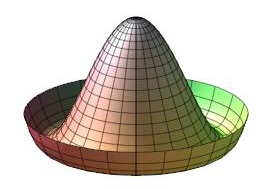
\includegraphics[width=0.5\textwidth]{Chapters/03_Theory/Images/higgspot}\hfill
     \caption[The Higgs field potential.]{The Higgs field potential $V(\Phi)$~\cite{Moss:2015fma}.}
     \label{fig:higgs_potential}
\end{figure}

Terms known as Yukawa coupling terms can be introduced to specify the interactions of $\Phi$ with the fermion
fields. It is this coupling of the Higgs field to any massive particle that gives them a proportional mass.
The top quark, being the heaviest known particle at \textasciitilde173\GeV, has a Yukawa coupling to the
Higgs field close to 1.
%TODO: IMPORTANT BECAUSE?

Results published at the discovery of the Higgs boson are shown in Figure~\ref{fig:higgs_results} in the
Higgs$\rightarrow\gamma\gamma$ and Higgs$\rightarrow\Z\Z$ channels. These plots of the invariant masses of the
$\gamma\gamma$ and $\Z\Z$ combinations show a clear excess of events around 125\GeV. The latest results from
CMS and ATLAS state a Higgs mass of $125.09\pm0.21\pm0.11\GeV$~\cite{Aad:2015zhl}, where the first uncertainty
is statistical and the second is systematic. Since the announcement of the discovery of the Higgs boson in 2012,
studies have continued to determine its quantum properties. Thus far, results show it to be in agreement with
predictions from the Standard Model.

\begin{figure}[hbtp]
   \centering
     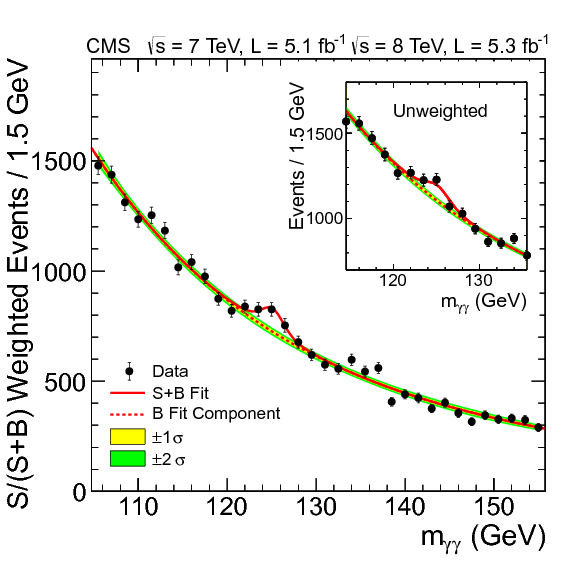
\includegraphics[width=0.5\textwidth]{Chapters/03_Theory/Images/sbweightedmassunweightedinset1_5GeV}\hfill
     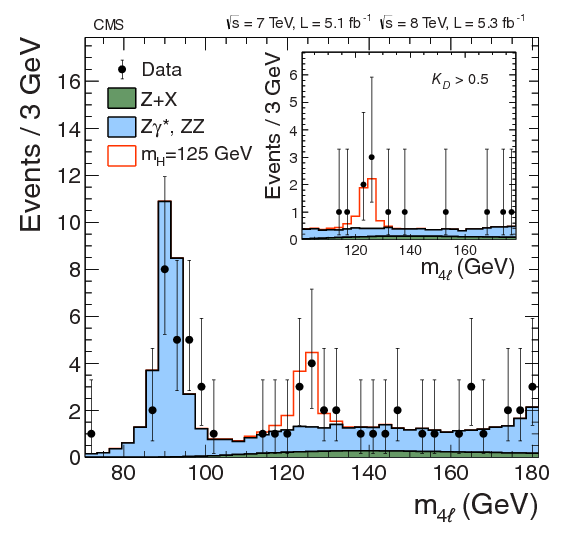
\includegraphics[width=0.5\textwidth]{Chapters/03_Theory/Images/H4l_mass_v3}\hfill
     \caption[Invariant mass in $H\rightarrow\gamma\gamma$ (left) and $H\rightarrow\Z\Z$ (right)
     channels.]{Invariant mass in $H\rightarrow\gamma\gamma$ (left) and $H\rightarrow\Z\Z$ (right) channels
     ~\cite{Chatrchyan:2012xdj}.}
     \label{fig:higgs_results}
\end{figure}

\section{Incompleteness of, and physics beyond, the SM}
\label{s:Incompleteness_of_and_physics_beyond_the_SM}
The Standard Model has proven to be an extremely successful theory thus far. However, its inability to
describe many phenomena in the universe lead to it being considered currently incomplete. Indeed, a `Grand
Unified Theory' combining the electromagnetic, weak and strong interactions is considered to be the next step
towards a `Theory of Everything' including gravity, with all of these forces being different physical
manifestations of one single force.

There are many free parameters in the Standard Model and the very reason why it takes the form it has, with
four fundamental forces, six quarks and six leptons, each divided into three generations, is not explained.
The gravitational force is also conspicuous by its absence from the SM. The imbalance between matter and
anti-matter in the universe, despite the generally accepted view that both were created in equal quantities in
the Big Bang, is also not fully explained by the SM. Although the evident matter-antimatter asymmetry in the
unvierse could be partially explained by the observed charge-parity (CP) symmetry violation in weak
interactions~\cite{Christenson:1964fg}, this is not sufficient to account for the observed excess.

Furthermore, the SM does not provide a theoretical explanation for neutrino mass. Originally thought to be
massless, neutrinos are now thought to have mass, albeit extremely small, based on observations of neutrino
oscillations between different flavours~\cite{Kajita:1998bw,Fukuda:1998mi}.

The hierarchy problem, in terms of the Higgs boson, refers to the fact that the measured Higgs mass is many
orders of magnitude smaller than the order of the Planck scale ($1.22\times10^{19}\GeV$). The expected
quadratically divergent quantum corrections to the Higgs mass from higher order interactions should result in
a far higher mass. This disagreement suggests that there occurs some `fine tuning' of the bare Higgs mass, to
lead to the experimentally observed mass of approximately 125\GeV.

Supersymmetry (SUSY) is one potential solution to hierarchy problem. This theory proposes a symmetry between
fermions (spin $\frac{1}{2}$) and bosons (spin 1). Each particle has an associated `superpartner' with
identical quantum properties with the exception of spin, which differs by $\frac{1}{2}$, so that all SM
fermions have a boson superpartner, and all SM bosons have a fermion superpartner.
These super particles, or sparticles, are thought to have higher masses than their SM counterparts since they
have not been discovered yet, making supersymmetry a broken symmetry. In many supersymmetry theories, the
lightest SUSY particle (LSP) is stable and is a potential candidate to be a dark matter particle.

Another potential solution is the theory of topcolor, an example of a composite model theory that suggests the
existence of a top-quark-condensate (a composite field of the top and antitop
quarks)~\cite{1990PhRvD..41.1647B,1991PhLB..266..419H} that acts effectively like the SM Higgs field. Such a
theory gives rise to a new fundamental interaction between top quarks at high energies resulting in the large
top mass. Theories of extra dimensions also exist, in which additional space-time dimensions are postulated in
which only gravity propagates~\cite{ArkaniHamed:1998rs}.
This could provide an explanation for the fact that the Planck scale is far larger than the electroweak force
by solving the heirarchy problem.

The universe is thought to constitute of about 27~\% dark matter, 68~\% dark energy and 5~\% ordinary
matter (Figure~\ref{fig:universe_composition})~\cite{Ade:2013sjv}. The origins and nature of the dark energy and dark
matter are currently unknown and they are as yet unobserved, but their existence has been inferred from their
gravitational effects on galactic masses composed of stars, gases and dust. The relatively large amounts of
dark matter and dark energy hypothesised suggests that they are made up of weakly interacting massive
particles.

\begin{figure}[hbtp]
   \centering
     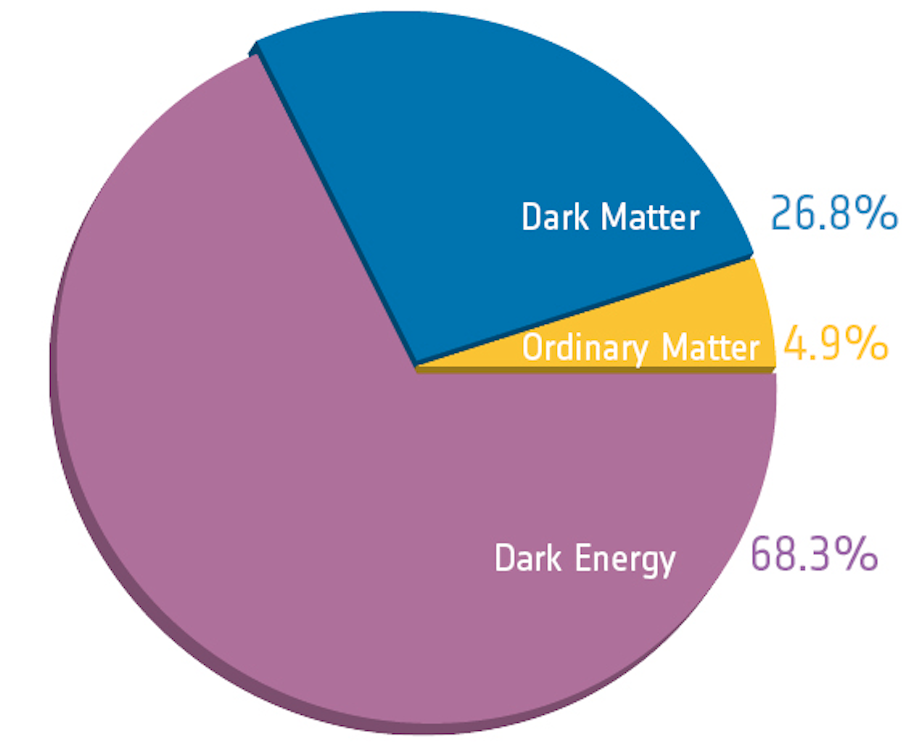
\includegraphics[width=0.5\textwidth]{Chapters/03_Theory/Images/planck_cosmic_pie}\hfill
     \caption[The composition of the universe showing the amounts of dark matter, dark energy and ordinary
     matter.]{The composition of the universe showing the amounts of dark matter, dark energy and ordinary
     matter based on latest results from Planck/ESA~\cite{Ade:2013sjv}}
     \label{fig:universe_composition}
\end{figure}

\chapter{Top Physics at the LHC}
\label{c:top_physics_at_the_lhc}

\section{Introduction}
\label{s:top_physics_intro}
The top quark was discovered by the CDF and D{\O} collaborations at the Tevatron at Fermilab in 1995
\cite{Abe:1995hr, Abachi:1995iq} and is still one of the less well studied fundamental particles in the
Standard Model. The top quark is the heaviest fermion with its mass currently placed at $173.29 \pm 0.23
(stat.) \pm 0.92 (syst.)\mathrm{~GeV/c^{2}}$ \cite{top_mass}. Since the lifetime of the top quark is very
short, approximately $5 \times 10^{25}\mathrm{~s}$ \cite{Agashe:2014kda}, it is the only one of the quarks to
decay before it hadronises, meaning that the bare quark properties can be investigated. These unique
properties of the top quark within the Standard Model mean it is an interesting focus of study.

\subsection{Top Quark Production and Decay}
\label{ss:top_quark_production_and_decay}
Top quarks can be produced either in top-antitop (\ttbar) production through the strong interaction or single
top (\tquark) production through the electroweak mechanism. During Run 1 of data taking at the LHC produced
millions of top quark pair events with gluon-gluon fusion or quark-antiquark annihilation being the primary
production mechanisms, as shown in Figure~\ref{fig:ttbar_production}. Gluon-gluon fusion dominates at the LHC
since protons are collided with protons, meaning antiquarks are only available from sea quarks in the proton.
In addition, at low momentum fractions, $x$, the gluon density in the proton is large compared to the sea
quarks, and increases at a higher rate than that of the sea quarks. TODO: COULD INSERT PLOT OF PROTON
PDFs IF NEEDED %TODO: COULD INSERT PLOT OF PROTON PDFs IF NECESSARY.

\begin{figure}[hbtp]
   \centering
     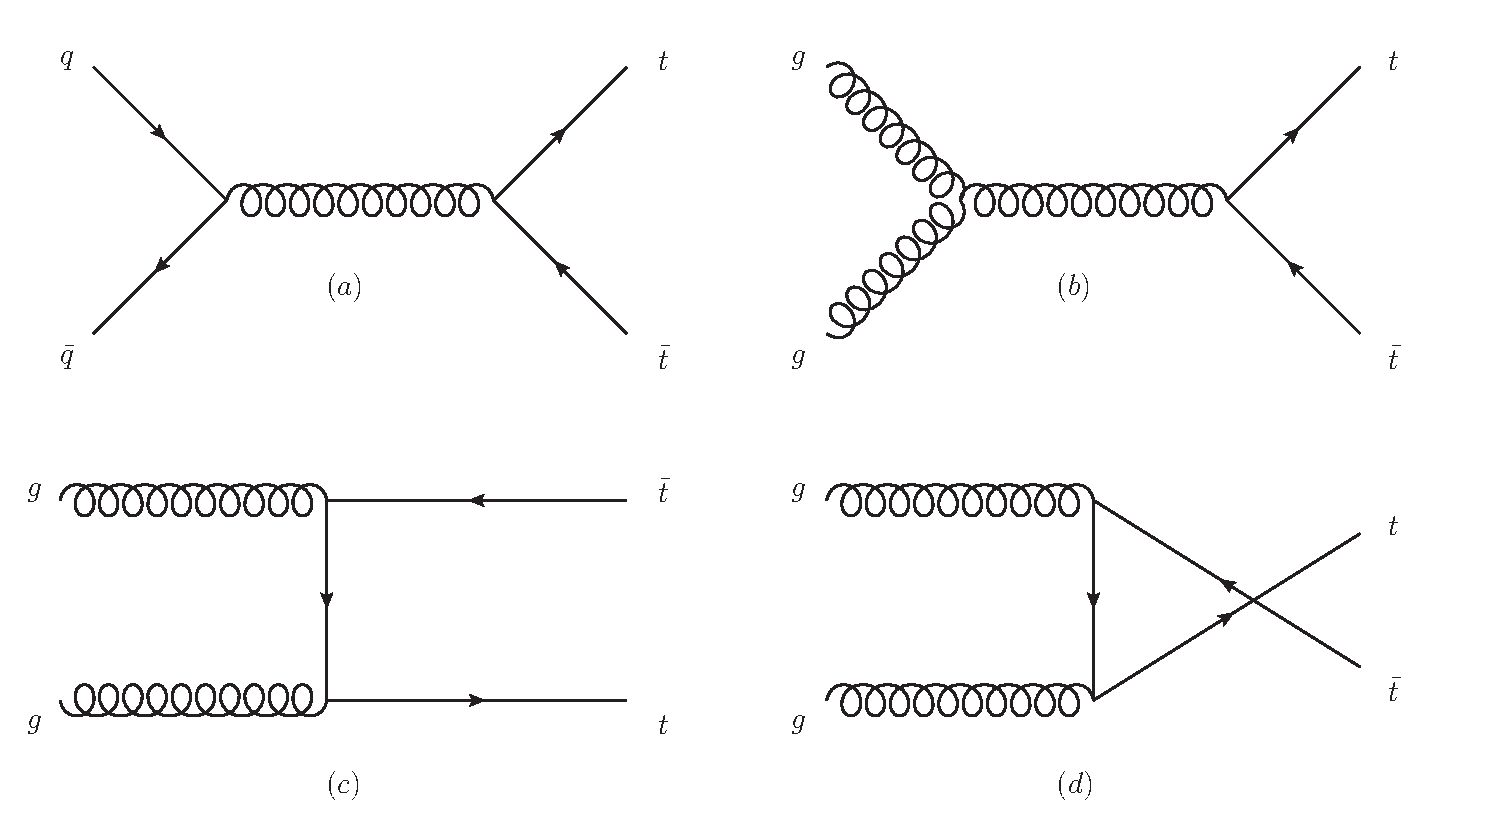
\includegraphics[width=0.9\textwidth]{Chapters/03_Theory/Images/ttbar_production}\hfill
     \caption[Feynman diagrams of leading order \ttbar production processes.]{Feynman diagrams of leading
     order \ttbar production processes. (a) depicts quark-antiquark annihilation, and (b, (c) and (d) depict
     gluon-gluon fusion in the s, t and u channels respectively.)}
     \label{fig:ttbar_production}
\end{figure}

At $\sqrt{s}=7\TeV$, gluon-gluon fusion accounts for approximately 80\% of the total \tquark production cross
section, increasing to approximately 90\% at $\sqrt{s}=14\TeV$ \cite{Agashe:2014kda}.
% A \ttbar production cross section of has been measured at $\sqrt{s}=7\TeV$ and at $\sqrt{s}=8\TeV$.

\begin{figure}[hbtp]
   \centering
     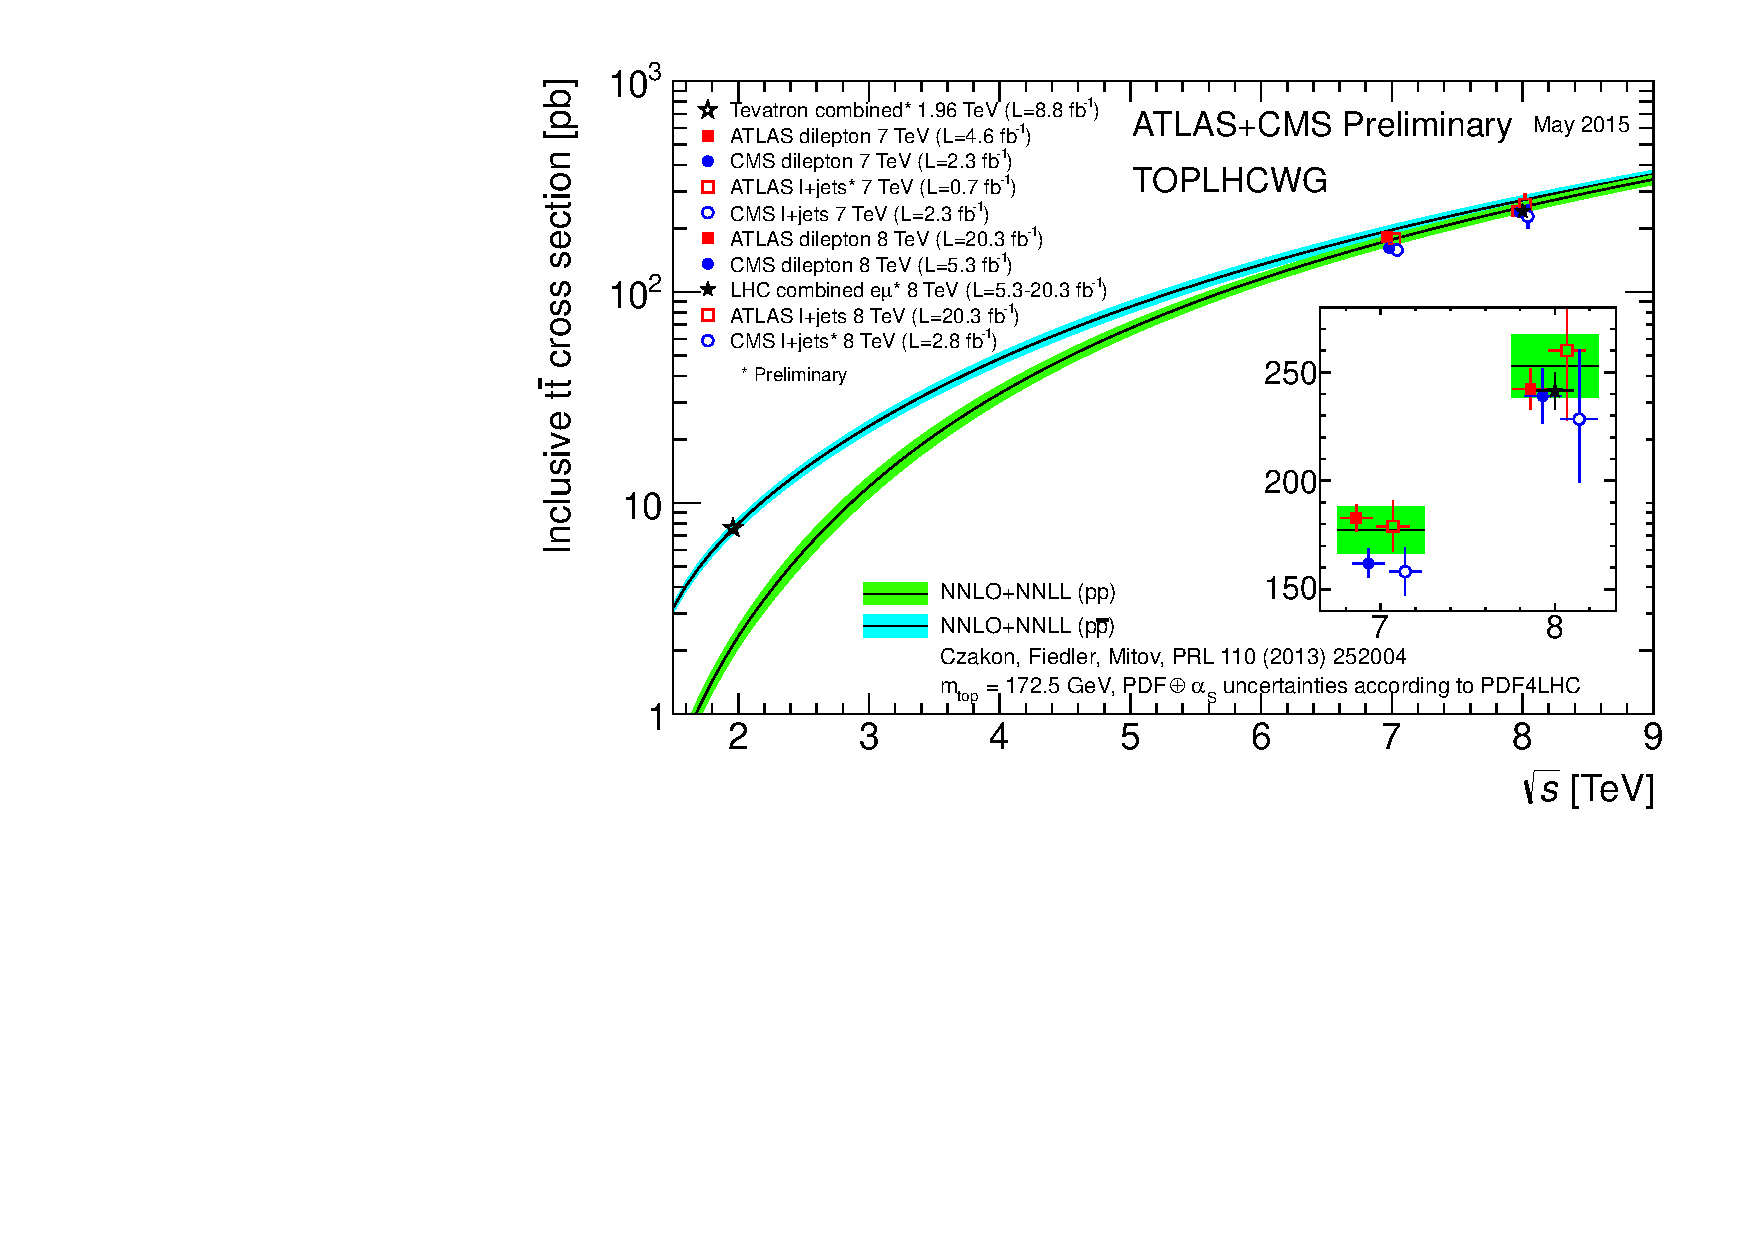
\includegraphics[width=0.5\textwidth]{Chapters/03_Theory/Images/toplhcwg_ttxsec_sqrts_may2015}\hfill
     \caption[\ttbar production cross sections at 1.96\TeV at CDF and D{\O} at the TeVatron and at 7\TeV and
     8\TeV at CMS and ATLAS at the LHC.]{\ttbar production cross sections at 1.96\TeV at CDF and D{\O} at the
     TeVatron and at 7\TeV and 8\TeV at CMS and ATLAS at the LHC. HOW REFERENCE IMAGE FROM
     https://twiki.cern.ch/twiki/bin/view/LHCPhysics/TopLHCWGSummaryPlots?}
     \label{fig:ttbar_cross_sections}
\end{figure}

Top quarks decay almost 100\% of the time to a \W boson and a \cPqb flavour jet. The \W boson then decays
either hadronically (into two jets) or leptonically (lepton + neutrino). Top pair events are characterised by the
decay of the \W bosons:
\begin{itemize}
  \item Leptonic: $\ttbar \rightarrow \W^{+} \cPqb \W^{-} \cPaqb \rightarrow l \nu_{l}\cPqb
  l' \bar{\nu_{l'}} \cPaqb$.
  Both \W bosons decay to a lepton and a neutrino. The event would consist of 2 jets, 2 leptons and 2
  neutrinos (which would show up as \met in the event). (10.5\%)
  \item Hadronic: $\ttbar \rightarrow \W^{+} \cPqb \W^{-} \cPaqb \rightarrow \cPq \cPaq \cPqb \cPq \cPaq
  \cPaqb$. Both \W bosons decay to two jets. The event would consist of 6 jets. (45.7\%)
  \item Semi-Leptonic: $\ttbar \rightarrow \W^{+} \cPqb \W^{-} \cPaqb \rightarrow \cPq \cPaq \cPqb l \nu_{l}
  \cPaqb$. One \W boson decays to a lepton and a neutrino, the other decays to two jets. The event would
  consist of 4 jets, 1 lepton and 1 neutrino. This decay is shown in Figure~\ref{fig:semileptonic_decay}.
  (43.8\%)
\end{itemize}

\begin{figure}[hbtp]
   \centering
     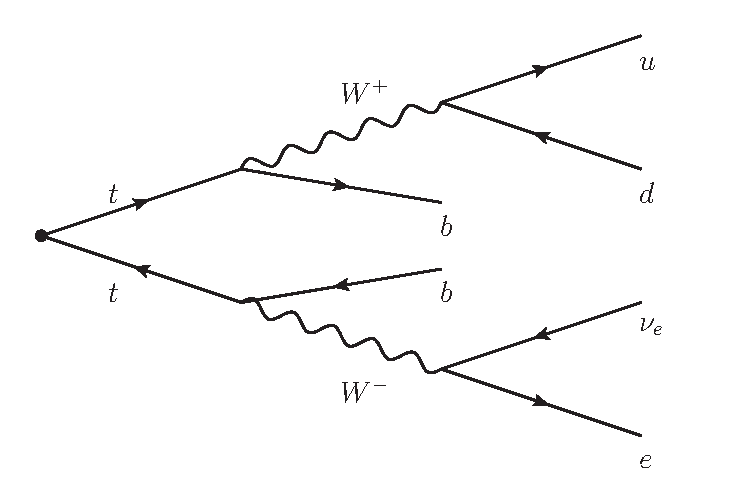
\includegraphics[width=0.5\textwidth]{Chapters/03_Theory/Images/semileptonic_decay}\hfill
     \caption[Feynman diagram of the electron+jets semi-leptonic \ttbar decay channel.]{Feynman diagram of the
     electron+jets semi-leptonic \ttbar decay channel.}
     \label{fig:semileptonic_decay}
\end{figure}

The branching ratios for each decay mode are quoted in brackets \cite{Agashe:2014kda}, and are represented
graphically in Figure~\ref{fig:ttbar_branching_ratios}. The numbers of jets in the final state of each channel
could be higher than the numbers quoted above as a result of higher order processes such as initial state
radiation (radiation from the gluons before the \ttbar production) or final state radiation. The hadronic
decay channel, with multiple jets and no leptons in the final state, is difficult to distinguish from the QCD
multijet, W+jets and Z+jets backgrounds. Conversely, the leptonic channel has a very clean signature with two
leptons, however the low branching ratio would limit the available statistics. The semi-leptonic channel, with
one lepton and four jets provides a good balance between statistics and event identification. The lepton can
be any of an electron, muon or $\tau$, but $\tau$s are not included in semi-leptonic \tquark analyses in
general as they are difficult to identify (see Section~\ref{ss:experimental_uncertainties}).

\begin{figure}[hbtp]
   \centering
     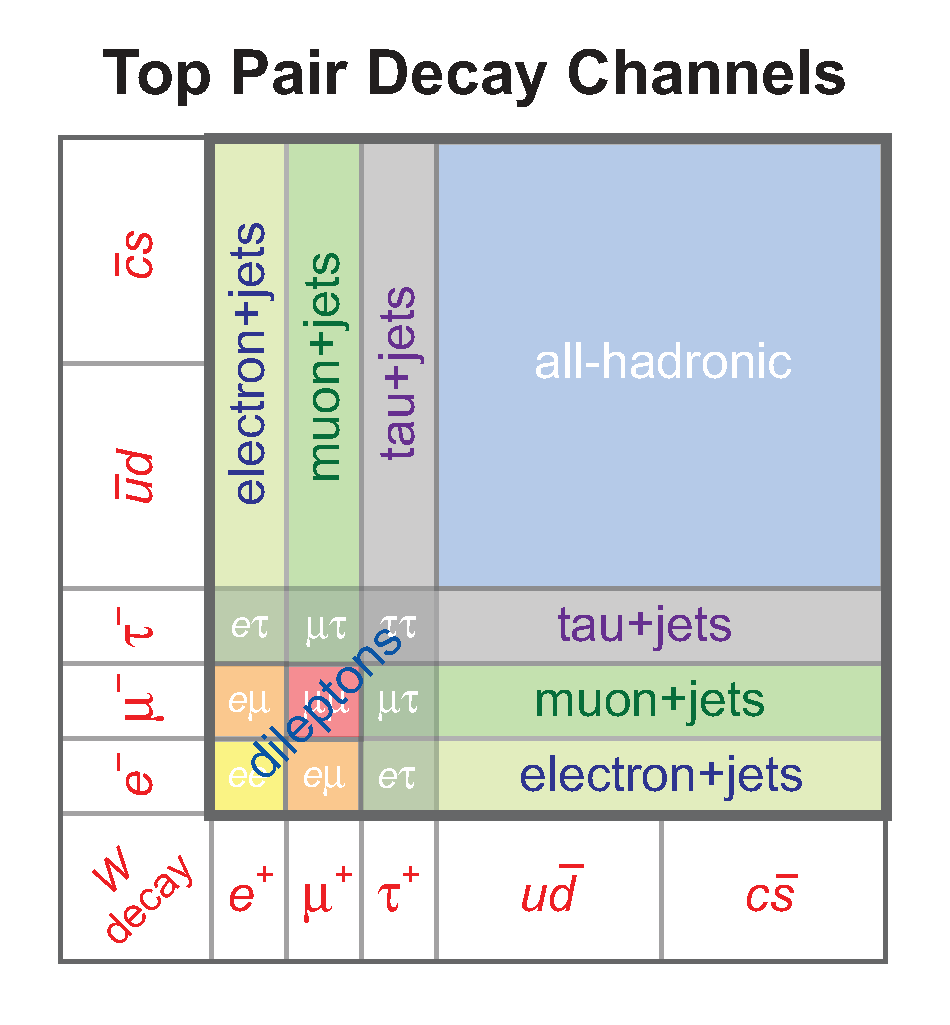
\includegraphics[width=0.5\textwidth]{Chapters/03_Theory/Images/top_pair_decay_channels.eps}\hfill
     \caption[Relative branching ratios of the \ttbar system]{Relative branching ratios of the \ttbar system}
     \label{fig:ttbar_branching_ratios}
\end{figure}

The signal event for this analysis is the semi-leptonic channel of the \ttbar decay, also referred to as
the lepton+jets channel, where the lepton is either an electron or a muon. These channels have a branching
ratio of apprimxately 14.2~\% and 14.4~\% respectively \cite{Agashe:2014kda}.

\subsection{Single Top background}
\label{ss:single_top}
Single top production is one of the backgrounds considered in this analysis, and can occur via the electroweak
interaction in one of three channels: s-channel or t-channel which involve the exchange of a virtual \W boson,
or tW-channel which involves the associated production of a \W boson and a top quark. Although semi-leptonic
\ttbar decays have more jets in the final state than these single top production modes, initial state
radiation and final state radiation, where low energy gluons and quarks are produced before and after the
interaction that produces the single \t quark, can increase the numbers of jets in single top events. This can
lead to such events having a similar signature to \ttbar events, and providing a non-negligble background.

\subsection{W/Z+jets background}
\label{ss:w_z_plus_jets}
\WpJets events present a significant background to semi-leptonic \ttbar analyses. This background consists of
events in which a real \W boson is produced together with additional jets. Events in which these \W bosons
decay leptonically, can provide a similar event signature after reconstruction to that of a semi-leptonic
\ttbar decay. However, in general, these processes can be removed from the signal selection because the final
decay products in \WpJets events typically have lower energies than those from semi-leptonic \ttbar decays,
since the top quark has a high mass. Another characteristic of \WpJets events is that the jets are more likely
to be light quark jets and therefore less likely to be \bjets than in \ttbar events. Thus, \WpJets events can
be separated from the \ttbar signal by using jet multiplicity, jet \pt and \bjet multiplicity.

Similarly, \ZpJets events can mimic \ttbar events where the leptonic decay of a \Z boson to a lepton and an
anti-lepton takes place. This background can be distinguished and removed from semi-leptonic \ttbar decays by
vetoing on a second lepton and imposing jet multiplicity requirements. Misidentification and misreconstruction
of these leptons as jets, however, can result in such events mimicking \ttbar events and passing the signal
selection, although this contamination is small.

\subsection{QCD background}
\label{ss:qcd}
The multi-jet background from QCD events is also a significant background to this semi-leptonic \ttbar
analysis. Gluon-gluon fusion and quark-antiquark annihilation in proton-proton collisions can produce
energetic jets. Although these processes have only two jets in their final state, higher order processes,
including initial state radiation and final state radiation, can also produce additional jets, leading to
potential mimicking of the semi-leptonic \ttbar signal. The leptons required for this to happen can come from
jets which are misreconstructed and misidentified as leptons, or real leptons in heavy flavour (\cPqb and
\cPqc flavour) jets. Unfortunately the cross section of these processes is several orders of magnitude larger
than the signal cross section. Although the lepton (either fake or real) is rarely one that passes selection,
the much higher QCD cross section means that its contribution as a background is significant.
% TODO: READ LUKE'S THESIS FOR WAYS IN WHICH JETS CAN FAKE AN ELECTRON OR A MUON

In the muon+jets channel, only highly energetic jets (\pt$>$500~\GeV) are capable of ``punching through''
from the calorimeters to leave tracks in the muon chambers. Such events can be removed by isolation (since it
deposits significant amounts of energy in the calorimeters) requirements. Events with real electrons and muons
from heavy quark jets can be identified by the track quality requirements in the selection since they would
not begin from the primary vertex and so would have a distrinct track signature compared to prompt leptons.

On the other hand, the electron channel poses a more problematic QCD background, due mainly to the conversion
of photons, whether produced at the interaction point or through subsequent decays and radiation, into
electrons and positrons. The identification and removal of such events is described in
Section~\ref{ss:electron_reconstruction}. However, the large uncertainty in the cross section of QCD events,
large contamination from higher order processes with additional jets in the signal region of this analysis and
the difficulty in Monte Carlo modelling of such contributions lead to significant disagreements in the numbers
of events passing the signal selection in data and in simulation. Therefore, the QCD background is modelled
using a data driven method.

The QCD background is difficult to model precisely because of large uncertainties on the cross sections and
the significant higher contributions which can easily be mismodelled, leading to incorrect event kinematics
and selection biases. Hence, the QCD background shape is modelled using a data driven method, decribed in
Section~\ref{ss:background_selection} and then normalised to the number of events passing the selection
process in Monte Carlo.

\section{Monte Carlo Simulation}
\label{s:monte_carlo_simulation}

Monte Carlo event simulation is used to simulate the aforementioned signal and background processes, and to
compare the theoretical knowledge of the Standard Model incorporated therein with real data. Differences
between simulation and data would then indicate the presence of new physics processes which are not present in
the theoretical assumptions made in the Standard Model, or perhaps that the simulation process is sub-optimal.
Different event generators exist, and samples produced by the \MADGRAPH, \PYTHIA, \POWHEG and \HERWIG
generators are used in this analysis.

Different generators have characteristics which optimise them for different aspects of the production chain:
the initial hard process scattering of the partons in the hadrons (protons), decay showers of the resulting
partons, subsequent decays of resulting hadrons and hadronisation of resulting partons, and the underlying
event (the parton showers produced from soft scattering between the remaining contents of the colliding
protons). 

\subsection{MadGraph}
\label{ss:madgraph}
\MADGRAPH \cite{madgraph5}, a matrix element generator, works by taking into account every potential Feynman
diagram for a given process and subsequently calculating the matrix elements for said diagrams over all phase
space. The parton distribution functions are used to generate the incoming partons. The cross section of the
process and various subprocesses and the structure and contents of the event (such as the partons present and
their kinematics) are thus produced. %Also spin correlations. Also tau
% lepton decays
Proton fragmentation and subsequent hadronisation are simulated using the \PYTHIA generator, as explained in
Section~\ref{ss:pythia}. The parton showers are then matched with the matrix element partons via the MLM
method ~\cite{mlm}. This method ensures that parton showers with a highly energetic jet are not double
counted.

Matching is then carried out between parton showers in the hadronisation and the partons from the matrix
element calculations. The matching is carried out by satisfying distance requirements in $\eta$ and $\phi$
between the parton and parton shower. Only if the parton has a transverse energy above a certain threshold, is
it considered for this matching, and if an event contains either too few or too many matching jets, it is
discarded. The matching threshold is process dependent as follows:
\begin{itemize}
  \item \ttbar: 20\GeV
  \item \WpJets: 10\GeV
  \item \ZpJets: 10\GeV
\end{itemize}

\subsection{MCatNLO}
\label{ss:mcatnlo}
The \MCATNLO \cite{mcatnlo_Frixione1, mcatnlo_Frixione2} generator is a next-to-leading-order generator. These
aditional corrections provide more accurate simulations of physics processes in comparison to leading-order
generators by including additional partons from the initial hard process in the final state of the event.

\subsection{PYTHIA}
\label{ss:pythia}
\PYTHIA \cite{pythia8} then simulates the proton fragmentation, the subsequent hadronisation of the
resulting quarks and gluons resulting from the hard interaction and the underlying event. \PYTHIA is
considered to be particuarly good at multi-particle simulation, modelling fragmentation and hadronisation, and
matching parton showers. Therefore, \PYTHIA carries out these steps after the initial partons are provided
by other generators in most simulated samples, if it is not already used for the whole production chain (as is
common in QCD multijet simulations).

\subsection{POWHEG}
\label{ss:powheg}
One problem with the \MCATNLO generator is that some events are given negative weights when matching
the next-to-leading-order QCD multijet calculations to parton showers.  The Positive Weight Hardest Emission
Generator, \POWHEG \cite{powheg_Frixione, powheg_Nason, powheg_Alioli}, is another next-to-leading-order
generator which generates the hardest processes in the event first, which avoids double counting of
softer radiation produced later in the chain, which is the cause of negative event weights.

%\subsection{HERWIG}
%\label{ss:herwig}
%\HERWIG \cite{herwig}
%TODO:HERWIG

\section{Theoretical Systematics}
\label{s:Theoretical Systematics}
\subsection{Factorisation \& Matching Threshold}
\label{ss:factorisation_and_matching_threshold}
Systematic uncertainties are present in the choice of the threshold transverse energy above which matching of
matrix-element partons to parton showers is carried out. Simulated samples in which the threshold is
increased and decreased by a factor of 2, are used to estimate the affect of this uncertainty on this
analysis:

\begin{itemize}
  \item \ttbar
  \begin{itemize}
    \item + variation: 40\GeV
    \item - variation: 10\GeV
  \end{itemize}
  
  \item \WpJets
  \begin{itemize}
    \item + variation: 20\GeV
    \item - variation: 5\GeV
  \end{itemize}

  \item \ZpJets
  \begin{itemize}
    \item + variation: 20\GeV
    \item - variation: 5\GeV
  \end{itemize}
\end{itemize}

Similarly, the factorisation scale at which $\alpha_{S}$ is varied up and down from the nominal value of
$Q^{2} = m^{2} + \Sigma p_{T}^{2}$ by a factor of 2 to produce simulation samples to evaluate the sytematic
uncertainty resulting from this. The uncertainty resulting from these variations are evaluated in both \ttbar
and \W/\ZpJets processes.
% TODO SMALL TABLE OF 0.5x and 2x variations?

\subsection{Detector Simulation (GEANT)}
\label{ss:detector_simulation}
Following creation of the physics processes in proton-proton collisions, the simulated events are then put
through a detector simulation to evaluate the interation of the detector with the products of collisions. The
Geometry and Tracking 4 (\GEANTfour) package is used for this purpose, which generally simulates what happens
to particles as they travel through the geometry of the detector, including simulation of the detector
components and materials and the interaction of particles with the detector such as particle tracks and energy
deposits.
\chapter{\btagging Study}
\label{c:b_tagging_study}

The decay of the \tquark to a \W boson and a \bquark necessitates a thorough understanding of these decay
products in \ttbar events. In particular, methods to identify jets coming from a \bquark, known as \btagging,
are commonly used to increase the efficiency of $\tquark\rightarrow\bquark\W$ signal selection. CMS has
several algorithms for \btagging: TrackCounting (High Efficiency) and TrackCounting (High Purity),
JetBProbability; JetProbability; SoftMuon; SoftMuonByPt; SoftMuonByIP3d; SimpleSecondaryVertex (High
Efficiency); SimpleSecondaryVertex (High Purity); CombinedSecondaryVertex and CombinedSecondaryVetexMVA. These
algorithms produce a discriminator output for each jet which indicates how likely it is to be a \bquark
flavour jet. In all cases, a more positive discriminator value indicates a jet that is more likely to be a
\bquark flavour jet.

The relatively long lifetime (of the order of $10^{-12}\s$) of \bquarks means that they travel a significant
distance (of the order of a few \mm) before decaying. This leads to events with \bjets possessing a secondary
vertex at a distinguishable distance from the primary interaction vertex, as seen in
Figure~\ref{fig:secondary_vertex}. This secondary vertex information, together with track based information
such as the number of tracks in the jet, the invariant mass of the secondary vertex and the impact parameter
significance (described below) of each jet track, is used by the CSV algorithm to produce a discriminator
ranging from 0 to 1, with larger numbers corresponding to a higher probability of a jet being a \bjet. Three
\btagging working points are used in CMS: tight, medium and loose. The medium working point is used in the
different cross sections analysis, which carries a 1~\% mis-tag rate (the rate at which non-\bjets are
mistakenly tagged as \bjets) and approximately 70~\% \btag efficiency.
The tight and loose working points have mis-tag rates of 0.1~\% and 10~\%
respectively~\cite{Chatrchyan:2012jua}.

\begin{figure}[hbtp]
   \centering
     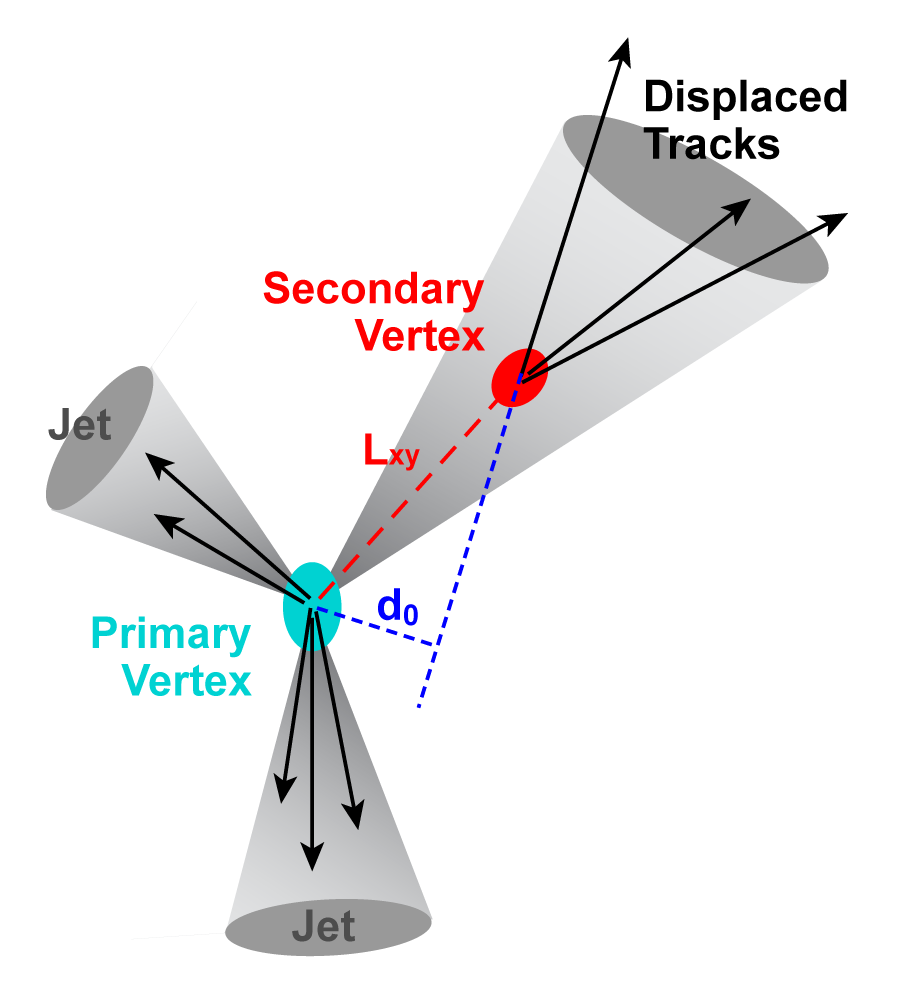
\includegraphics[width=0.8\textwidth]{Chapters/04_Analysis/04a_BTags/Images/b_tagging_graphic}\\
     \caption[Graphical representation of a secondary vertex.]{Graphical representation of an
     interaction originating at the primary vertex producing three jets, one of which is a \bjet with a
     secondary vertex~\cite{d0_fnal}.}
     \label{fig:secondary_vertex}
\end{figure}

\section{Observables used in \btagging algorithms}
\label{s:observables_used_in_btagging_algorithms}

The impact parameter (IP) of a track is defined as the distance between the track and the vertex at the point
of closest approach~\cite{CMS-PAS-BTV-09-001}. Figure~\ref{fig:impact_parameter} shows a schematic
representation of the impact parameter for one single track. The IP measurement can be made in either the
plane transverse to the beam line, or in three dimensions. The impact parameter significance
(IP/$\sigma_{IP}$) is often used instead as an input to \btagging algorithms to allow for the experimental
resolution, due to the fact that the uncertainty on the IP value alone can be as large as the IP itself. The
IP significance distribution of light jets ($\cPqu$, $\cPqd$, $\cPqs$) and gluon jets form a Gaussian
distribution about a mean of zero and width of one, with a slightly extended tail due to tracks from particles
in the jet with long lifetimes. The equivalent distribution for \cjets and \bjets show an asymmetric
distribution at positive values due to the long lifetime of B and C hadrons, making the IP significance a
useful parameter to distinguish between light and heavy flavour jets~\cite{CMS-AN-2005-041}.

The signed IP is also used, in which the sign is obtained from the sign of the scalar product of the IP vector
and the jet direction, so that it is positive if the angle between the IP vector and the jet direction is less
than 90$^{\circ}$, and negative if the angle is greater than 90$^{\circ}$. Tracks belonging in a \bjet would
have an IP sign >0, since the jet direction is an estimate of the direction of travel of the B hadron.
However, the sign could be inaccurately calculated in cases with badly reconstructed jet directions or primary
vertices, or badly measured track parameters~\cite{CMS-AN-2005-041}. Another parameter based on track length,
the 3D decay length significance (the ratio of the three dimensional distance between the primary vertex and
the secondary vertex, and the uncertainty on this value) is also used by some \btagging algorithms.

\begin{figure}[hbtp]
   \centering
     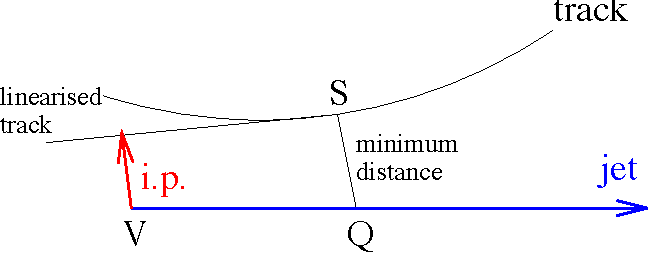
\includegraphics[width=0.8\textwidth]{Chapters/04_Analysis/04a_BTags/Images/impact_parameter}\\
     \caption[Graphical representation of a track impact parameter.]{Graphical representation of a track
     impact parameter~\cite{CMS-PAS-BTV-09-001}.}
     \label{fig:impact_parameter}
\end{figure}

Identification of vertices in CMS consists of two stages: vertex finding and vertex fitting. Vertex finding
deals with the creation of vertex candidates by grouping reconstructed tracks together. Vertex fitting then
deals with obtaining the vertex parameters such as position of the vertex and track parameters, and the
quality of the fit. An adaptive vertex fitter~\cite{0954-3899-34-12-N01} calculates an estimate of the vertex
position and weights tracks based on their compatibility with the vertex. This first fit is constrained to the
interaction region to identify prompt tracks. After removing tracks with weights >0.5, subsequent fits are
carried out to identify potential decay vertices, until no new vertex is identified.

\section{\btagging algorithm descriptions}
\label{s:btagging_algorithm_descriptions}

\subsection*{Track Counting}
\label{ss:track_counting}
The simplest \btagging algorithms available in CMS are the track counting
algorithms~\cite{CMS-PAS-BTV-09-001}, which positively identifies a \bjet if it contains N or more tracks with
IP significance above some theshold value. They function by ordering all good tracks in a jet by order of
decreasing IP significance, with the discriminator being the IP significance of the Nth track. The high
efficiency version of this algorithm uses N=2, i.e. the second track, and the high purity version uses N=3,
i.e. the third track~\cite{CMS-AN-2005-041}.

\subsection*{Jet Probability}
\label{ss:jet_probability}
The ``jet probability'' algorithms~\cite{CMS-PAS-BTV-09-001} produce a discriminator based on the probability that
the set of tracks come from the primary vertex: a high probability would indicate that the jet is not a \bjet,
which would originate at a secondary vertex. These algorithms use all tracks as input and for each track
define an individual probability of coming from the primary vertex. By combining these probabilities, a jet
probability is produced, and the discriminator is the negative log of this confidence
level~\cite{CMS-AN-2005-041}. The ``jet B probability'' variant is based on the four most displaced tracks in
the jet, since the mean number of tracks in a \bjet is approximately 5 and the reconstruction of tracks within
jets has an efficiency of approximately 0.8 in CMS~\cite{CMS-PAS-BTV-09-001}. The ``jet B probability'' in this
case is based on the confidence level that the four most displaced tracks originate from the primary vertex.

\subsection*{Soft Muon}
\label{ss:soft_muon}
The ``soft muon'' algorithms make use of global muons reconstructed in the vicinity of the reconstructed jet,
which may indicate a semi-leptonic decay of B hadrons to a muon~\cite{CMS-AN-2009-085}. Two soft muon
algorithms exist in CMS. The ``soft muon by \pt'' algorithm uses the relative \pt of the muon with respect to
the jet ($p_{T}{rel}$), which is expected to be larger than that for muons in light flavour jets due to the
large \bquark mass~\cite{CMS-AN-2009-085, Ferro:2012tg}. A ``soft muon by IP algorithm'' also exists which
uses the IP significance of positive IP muons. In jets containing more than one muon, the muon with the
highest discriminator is used.

\subsection*{Simple Secondary Vertex}
\label{ss:simple_secondary_vertex}
The simple secondary vertex (SSV) algorithm uses the Adaptive Vertex Fitter to reconstruct the secondary
vertex~\cite{0954-3899-34-12-N01}. The discriminator is calculated based on the 3D decay length significance.
If no secondary vertex is reconstructed, no discriminator is produced, meaning that the efficiency of this
algorithm is limited to the maximum efficiency of secondary vertex reconstruction (approximately
65~\%)~\cite{Chatrchyan:2012jua}. There are two variants of the simple secondary vertex algorithm: the high
efficiency version uses vertices with at least two compatible tracks, whereas the high purity version uses
vertices with at least three tracks. Since this algorithm does not directly use track-based lifetime
parameters, it is less sensitive than other algorithms to tracker misalignment.

\subsection*{Combined Secondary Vertex}
\label{ss:combined_secondary_vertex}
The current CMS recommendation for physics analyses (and therefore the algorithm used in the differential
cross section analysis presented in
Chapters~\ref{c:Differential_Cross_Section:data_simulation_and_selection}-\ref{c:Differential_Cross_Section:systematics_and_results})
is the Combined Secondary Vertex (CSV) algorithm~\cite{Weiser:2006md}. This algorithm reconstructs the event
vertices using the Trimmed Kalman Vertex Finder~\cite{Speer:927395}. This vertex finding algorithm fits tracks
to a primary vertex after removing incompatible tracks and applies cuts to these vertices in order to find a
secondary vertex. The CSV algorithm then combines track-based lifetime parameters, such as IP and flight
distance significance, with secondary vertex information to produce a discriminator. The increased number of
input parameters means that even in cases with no reconstructed secondary vertex a discriminator can be
produced, thereby increasing the maximum efficiency compared to the SSV algorithms~\cite{Chatrchyan:2012jua}.
A variant of this algorithm in which a multi-variate analysis (MVA) is performed using the CMSSW MVA Tools to
produce a discriminator.

\section{Performance Comparison}
\label{s:performance_comparison}

Distributions of the discriminators produced by the above algorithms were created for a \ttbar \MADGRAPH Monte
Carlo simulation sample (/TTJets\_TuneZ2\_7TeV-madgraph-tauola/, produced in the Fall2011 production cycle
using CMSSSW version 44X). A comparison of the discriminator distributions, after normalising to unit area,
for the described algorithms were carried out. Figure~\ref{fig:CSV_discriminators} shows a comparison between
the distributions obtained by the CSV algorithm for the different jets present in the sample: \bjets, light
jets (up, down and strange flavour: \udsjets), gluon jets (\gjets) and charm flavour jets (\cjets). All
distributions were normalised to unity in order to facilitate shape comparision. Equivalent plots for other
algorithms are included in Figure~\ref{fig:all_algorithm_discriminators} in Appendix~\ref{ac:b_tagging_plots}.
In all cases, it can be seen that higher discriminator values were produced for \bjets than for \udsjets,
\gjets and \cjets, as expected.

\begin{figure}[hbtp]
   \centering
     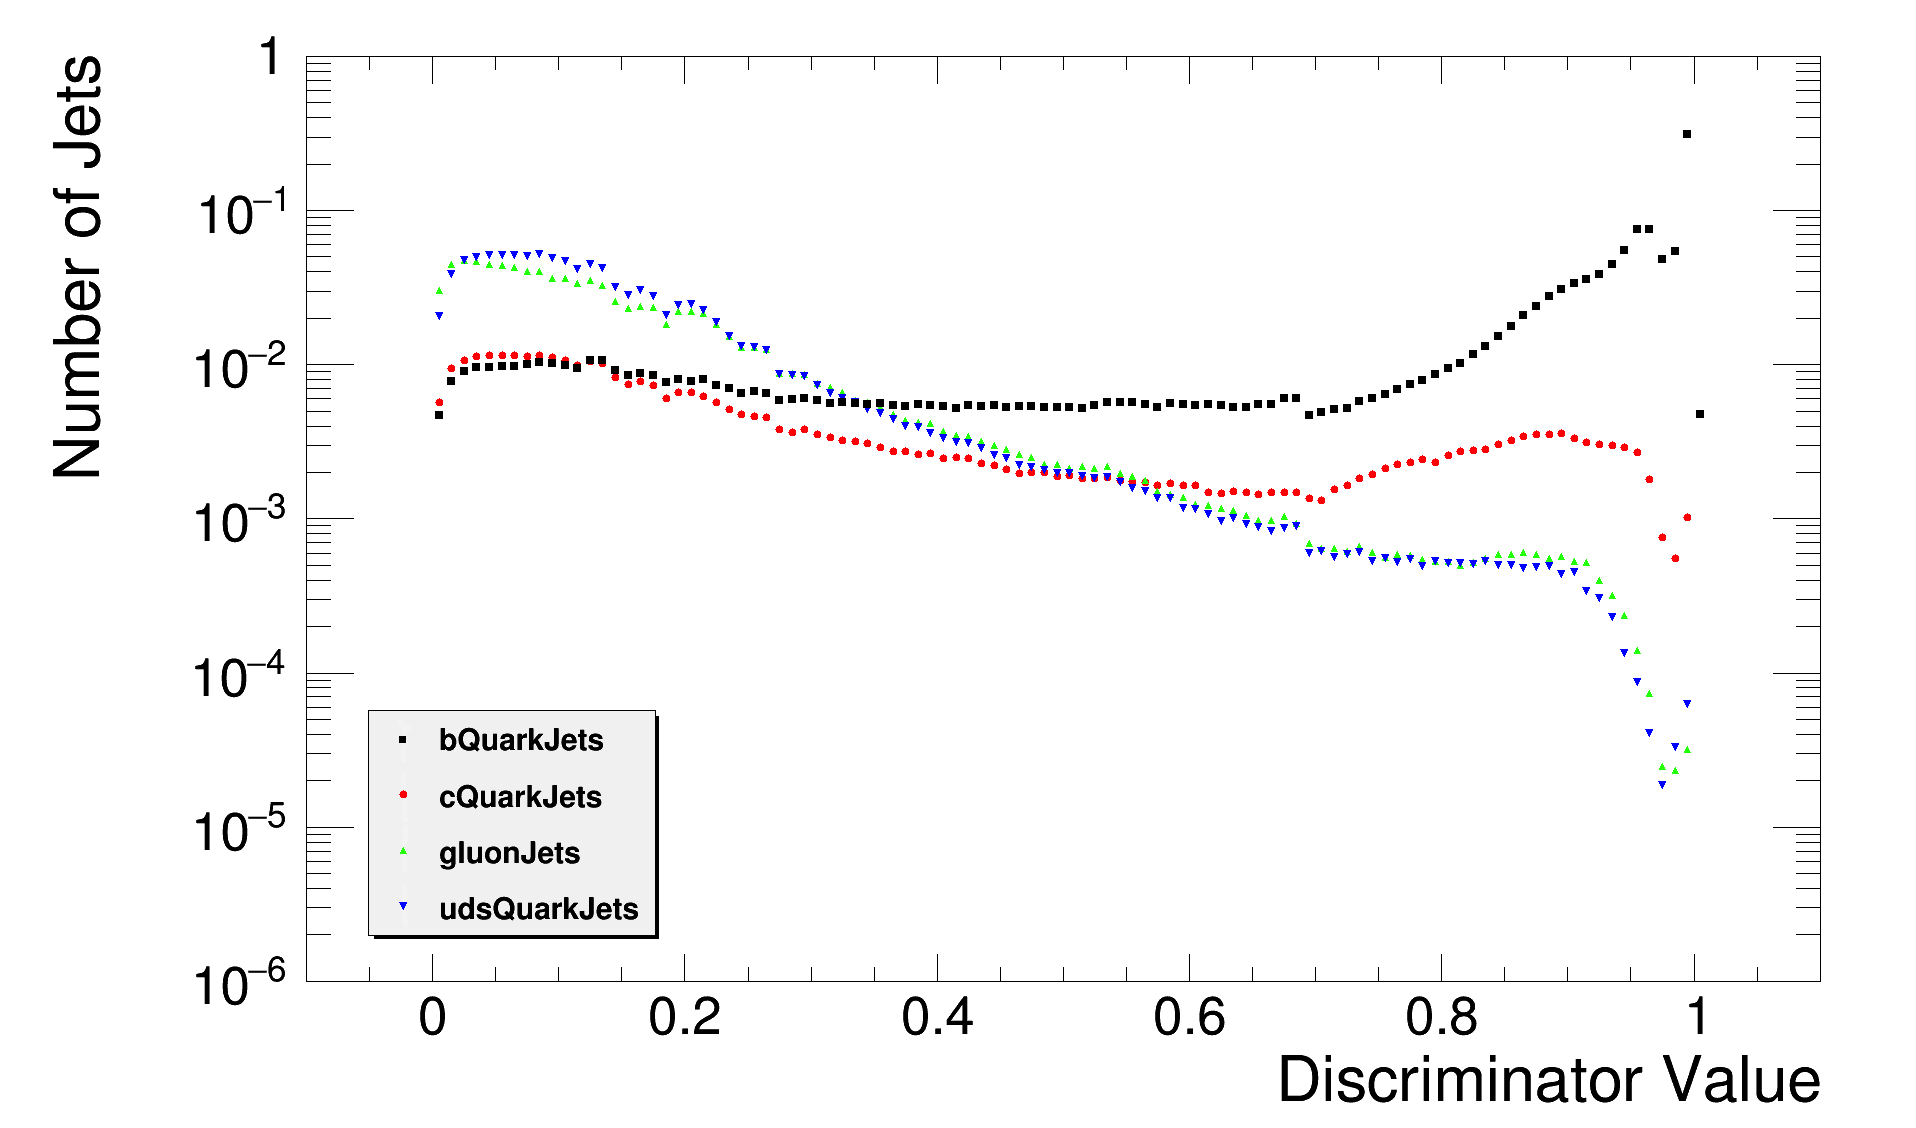
\includegraphics[width=\textwidth]{Chapters/04_Analysis/04a_BTags/Images/CombinedSecondaryVertex_norm_discriminator_combined}\\
     \caption[Discriminator values produced by the Combined Secondary Vertex algorithm after
     normalisation.]{Discriminator values produced by the Combined Secondary Vertex algorithm for all \bjets,
     \cjets, \gjets and \udsjets after normalisation.}
     \label{fig:CSV_discriminators}
\end{figure}

\section{Efficiency}
\label{s:efficiency}

Analyses in CMS make use of \btagging algorithms by placing cuts on the discriminators. The efficiency of a
cut can be defined as the ratio of number of jets passing the selection cut to the total number of jets before
the selection cut. The efficiency was calculated for cut values spanning the whole range of discriminator
values, thereby producing a plot of \btag efficiency as a function of CSV discriminator cut value
(Figure~\ref{fig:CSV_jet_efficiencies}). In practice, the aim is to acheive a high \bjet efficiency and a low
efficiency for all other jet flavours, \ie towards the bottom right of the plot. It can be seen that \udsjets
and \gjets have similar rates of increase in efficiencies with respect to cut value, owing to their similar
discriminator distributions. The \cjet discriminator distribution (Figure~\ref{fig:CSV_discriminators}),
however, has a noticeably different shape. This leads to the undesirable trend of higher \cjet efficiencies
than for \udsjets and \gjets. Equivalent plots for other algorithms can be found in
Figure~\ref{fig:all_algorithm_efficiencies} in Appendix~\ref{ac:b_tagging_plots}.

\begin{figure}[hbtp]
   \centering
     \includegraphics[width=\textwidth]{Chapters/04_Analysis/04a_BTags/Images/CombinedSecondaryVertex_nonBJetEfficiency_v_bJetEfficiency}\\
     \caption[Non \bjet efficiencies as a function of \bjet efficiency for the CSV algorithm.]{Non \bjet
     efficiencies as a function of \bjet efficiency for the CSV algorithm.}
     \label{fig:CSV_jet_efficiencies}
\end{figure}

\section{Algorithm Comparison}
\label{algorithm_comparison}

The performances of the various algorithms can be compared in Figure~\ref{fig:uds_eff_v_b_eff}.

\begin{figure}[hbtp]
   \centering
     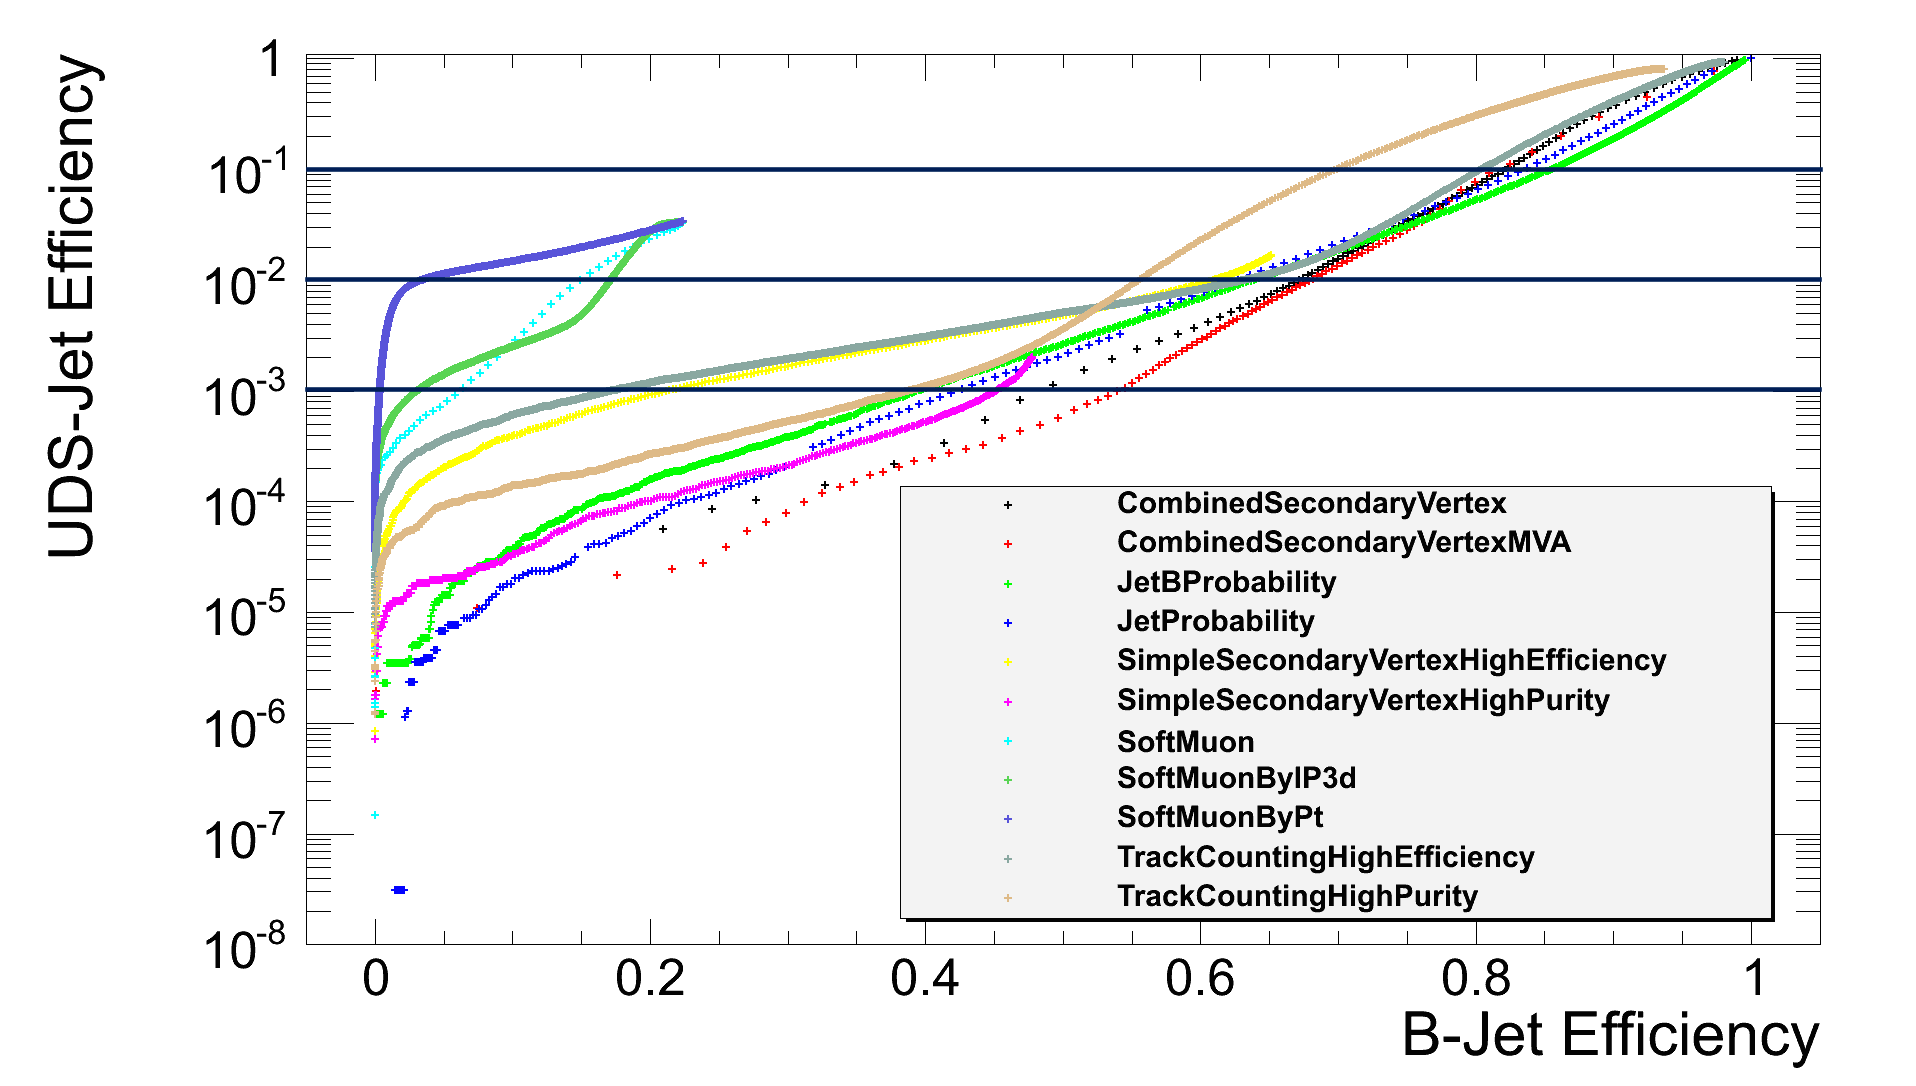
\includegraphics[width=\textwidth]{Chapters/04_Analysis/04a_BTags/Images/udsJetEfficiency_v_bJetEfficiency_withLegend_wp}\\
     \caption[udsjet efficiencies as a function of \bjet efficiencies for all algorithms.]{\udsjet
     efficiencies as a function of \bjet efficiencies for all algorithms.}
     %TODO: MAKE PLOT MORE LEGIBLE IF TIME PERMITS
     \label{fig:uds_eff_v_b_eff}
\end{figure}

It can be seen that not all algorithms reach 100~\% \bjet efficiency due to being inherently limited by their
methods. For example, the soft muon algorithms are limited by the muon identification efficiency within \bjets
and also by the branching fraction of B hadrons to muons. The soft muon algorithms all show low maximum \bjet
efficiencies due to the low B hadron semi-leptonic branching ratio to muons of approximately 11~\% (or 20~\%
when further decays are included such as $\cPqb \rightarrow \cPqc \rightarrow l$) \cite{Ferro:2012tg}.
Similarly, the SSV algorithms are limited by the efficiency of reconstructing a secondary vertex in the jet of
approximately 65~\%.

The 2011 and 2012 CMS recommended \btagger is the Combined Secondary Vertex with operating point discriminator
cuts of 0.244 (loose), 0.679 (medium) and 0.898 (tight) corresponding to 10\%, 1\% and 0.1\% light jet
efficiency. These cuts are indicated by the horizontal lines on Figure~\ref{fig:uds_eff_v_b_eff}. It can be
seen that for the tight and medium cuts, the CSV MVA algorithm provides the highest \bjet efficiency and
lowest light jet efficiency, followed closely by the CSV algorithm. The multiple variables that are used as
input allow the CSV algorithm to produce higher efficiencies than the SSV algorithms, while the MVA analysis
variant provides a slightly improved performance. At approximately 3\% light jet efficiency, there is a
convergence of many algorithms that all provide similar performance. At the loose working point also, many of
the algorithms provide similar performance with \bjets, with the ``jet probability'' algorithms marginally
outperforming the CSV algorithms. In early CMSSW versions, it was known that the jet probability algorithm
provided optimal performance, leading to it being recommended for early CMS analyses.
Ultimately, the CSV algorithm provides better performance in CMSSW versions after CMSSW\_2\_X\_Y, at which
point it became the recommended \btagging method.

\chapter{7 TeV and 8 TeV Differential Cross Section Measurement: Data, Simulation and Selection}
\label{c:Differential_Cross_Section:data_simulation_and_selection}

\section{Introduction}
\label{s:analysis1_introduction}
This analysis measures the normalised differential \ttbar cross section in the semi-leptonic channel and is
carried out on 2011 and 2012 data recorded from the CMS detector. The measurement is carried out with respect
to the following global, or primary, variables is carried out:
\begin {itemize}
  \item {\met, the missing transverse energy in an event}
  \item {\HT, the sum of the jet transverse momenta in an event}
  \item {\st, the sum of the observed transverse momenta in an event}
  \item {\mt, the transverse mass of the leptonically decaying \W boson}
  \item {\wpt, the transverse momentum of the leptonically decaying \W boson}
\end{itemize}

TODO:INCLUDE MT? %TODO: include MT?

Previous analyses using 7\TeV data investigating \met and using 8\TeV data investigatin all the
global variables listed above can be found in \cite{CMS-PAS-TOP-12-019} and \cite{CMS-PAS-TOP-12-042} respectively.

This investigation is motivated primarily by the importance of understanding \ttbar events since they are a
significant background in many new physics analyses. It is also helpful in understanding QCD and event
generators. Rare Standard Model processes such as $\ttbar + W\rightarrow l\nu$ or $\ttbar + Z\rightarrow
\nu\bar{\nu}$ would appear in \met distribution tail, and $\ttbar + X$ where $X$ is massive would appear in
the \HT and \st distributions. There are also possible new physics scenarios such as stop pair production,
$\tilde{t}\bar{\tilde{t}} \rightarrow t\tilde{\chi_0} \bar{t}\bar{\tilde{\chi_0}}$ which could show
hints of dark matter.

\section{Data and Simulated Samples}
\label{s:data_and_simulated_samples}

\subsection{Data}
\label{ss:data}

Data collected in 2011 at a centre-  of-mass energy of 7\TeV and in 2012 at a centre-of-mass energy of
8\TeV are used. The datasets are determined by the triggers that were used to record them. For 7\TeV, the ElectronHad
dataset is used in the electron channel. It was recorded with triggers that select based on a single, isolated
electron and additional jets. At 8\TeV, the SingleElectron dataset was used for the electron channel
which is based on a single, isolated electron. In the muon channel, the SingleMu dataset was used for both
centre-of-mass energies, requiring a single, isolated muon. See Section~\ref{s:selection} for more
details about triggers. The datasets used are shown in Tables~\ref{tab:datasets7TeV} and {tab:datasets8TeV} in
Appendix~\ref{as:datasets}. Only data that is certified as “golden”, which is defined as data taken with the
detector working without any major faults, used. The masks used to filter out data taken in other periods are
specified in Table~\ref{tab:JSONfiles} in Appendix~\ref{as:datasets}.

\subsection{Simulated Samples}
\label{ss:simulated_samples}
The Monte Carlo generators used in this analysis are MadGraph \cite{madgraph}, PYTHIA \cite{pythia8}, POWHEG
\cite{powheg_Nason,powheg_Frixione,powheg_Alioli}, HERWIG \cite{herwig} and MC$@$NLO
\cite{mcatnlo_Frixione1, mcatnlo_Frixione2}.

The signal for this analysis is the production of a \ttbar pair which decays semi-leptonically, \ie each of
the t quarks decays to a \W boson and a b jet, with one of the \W bosons decaying hadronically to two jets and
the other decaying leptonically to a lepton (electron or muon) and an associated neutrino.

Additional, lower energy jets, can be produced from other scatterings in the same proton-proton interaction
and from gluon radiation from quarks in the decay. Events with \W bosons or \Z bosons and additional jets are
a significant background to semi-leptonic \ttbar analyses. In the case of \W+jets, leptonically decaying \W
bosons and additional jets would provide a similar event signature to that of a semi-leptonic \ttbar decay.
However, in general, these processes can be removed from the signal selection because the final decay products
in \W+jets events have lower energies than those from semi-leptonic \ttbar decays, since the top quark has a
high mass. Another characteristic of \W+jets events is that the jets are less likely to be the necessary b
jets in \ttbar events. Similarly, \Z+jets events can mimic \ttbar events where the leptonic decay of \Z bosons
to a lepton and an anti-lepton. Within the framework of this analysis, prompt leptons are considered as those
which come from \W or \Z boson or from tau-lepton decays. These leptons are usually well isolated, whereas
misidentified leptons originate either from semi-leptonic heavy flavor decays within jets or are simply
misreconstructed genuine jets. In both cases these leptons are generally not isolated and a veto on a second
lepton together with jet multiplicity requirements removes much of this background. Misidentification and
misreconstruction of leptons as jets could still mean some of these events still pass the signal selection,
although this contamination would be small. TODO:FEYNMANN DIAGRAM OF W \& Z PRODUCTION.
% TODO: FEYNMANN DIAGRAM OF W & Z + JETS EVENTS



The QCD events that can form a background to \ttbar analyses, with the multi-jet final states resulting from
gluon-gluon fusion and quark-antiquark annihilation from proton proton collisions. At high orders, sufficient
numbers of jets can be produced to produce an event signature similar to that of \ttbar events. The leptons
required for this to happen can come from jets that are misreconstructed and misidentified as leptons, or from
the b and c quark decays. In the muon channel, it is possible to use isolation requirements to identify and
remove a jet of high enough energy that it leaves signals in the muon chambers, because it will also deposit
much energy in the calorimeters. Fake leptons caused by misreconstruction and misidentification, although not
a regular occurrence, form a significant background because the QCD cross section is large at the centre of
mass energies in this analysis. Fake leptons contained in b and c jets will not begin from the primary vertex
and so can be mostly excluded from the signal selection using their distinct track signature compared to prompt
leptons.

On the other hand, the electron channel poses a more problematic QCD background, due mainly to the conversion
of photons, whether produced at the interaction point or through subsequent decays and radiation, into
electrons and positrons. The identification and removal of such events has been described in
Section~\ref{ss:electron_reconstruction}. However, the large uncertainty in the cross section of QCD events,
large contamination from higher order processes with additional jets in the signal region of this analysis and
the difficulty in Monte Carlo modelling of such contributions lead to significant disagreements in the numbers
of events passing the signal selection in data and in simulation. Therefore, the QCD background is
modelled using a data driven method, decribed in Section~\ref{ss:background_selection}.

Tables~\ref{tab:signaldatasets7TeV} and \ref{tab:backgrounddatasets7TeV} show the Monte Carlo signal and
background samples respectively used in this analysis. Top pair production is modelled using MadGraph, single
top events are modelled with POWHEG, \W and \Z boson plus jets production is modelled using MadGraph and QCD
multi-jet events are modelled with PYTHIA. In all cases, PYTHIA is used to model radiation and hadronisation
processes. Tables~\ref{tab:7TeVsystematicdatasets} and \ref{tab:8TeVsystematicdatasets} show the samples used
to evaluate the factorisation scale and matching threshold uncertainties. \WpJets and \ZpJets samples were not made available at 7\TeV, so the
scaled distributions from \SI{8}{\TeV} were used, as described in Section~\ref{ss:7TeV_vplusjets_template}.

\begin{table}[hbth]
\centering
\caption{\SI{7}{\TeV} Monte Carlo signal datasets used for this analysis.}
\label{tab:signaldatasets7TeV} \small\addtolength{\tabcolsep}{-5pt}
\begin{tabular}{llrrr}
%\multicolumn{6}{c}{Signal datasets}
%\hline
Process & Generator & $\sigma$ ($\pb$) & No. events & \lumiint ($\fbinv$) \\
\hline
\ttbar & \MADGRAPH & 177.31 & 17100187 & 96.4 \\
\ttbar & \MCATNLO & Not Available & - & - \\
\ttbar & \POWHEG-\PYTHIA & 177.31 & 4833135 & 27.3 \\
\ttbar & \POWHEG-\HERWIG & 177.31 & 4480816 & 25.3 \\
\hline
\end{tabular}
\end{table}


\begin{table}[hbth]
\centering
\caption{\SI{7}{\TeV} Monte Carlo background datasets used for this analysis. All samples are generated
inclusively if not marked otherwise ($^\star$ generator cut on in-flight-decays of b- and c-hadrons, $^\ominus$ enriched in conversion electrons; $l$ means
all leptonic decays: $l=e,\mu,\tau$; $^\bullet$ generator cut on $m_{Z/\gamma} > 50$~GeV).
\label{tab:backgrounddatasets7TeV}} \small\addtolength{\tabcolsep}{-5pt}
\begin{tabular}{llrrr}
%\multicolumn{6}{c}{Background datasets} 
%\hline
Process & Generator & $\sigma$ ($\pb$) & No. events & \lumiint ($\fbinv$) \\
\hline
\hline
Single \t t-channel ($W\rightarrow l\nu$) & \POWHEG & 64.6 & 3249530 & 50.3 \\
Single \cPaqt t-channel ($W\rightarrow l\nu$) & \POWHEG & 64.6 & 1813615 & 28.1 \\
Single \t s-channel ($W\rightarrow l\nu$) & \POWHEG & 4.21 & 229786 & 54.6 \\
Single \cPaqt s-channel ($W\rightarrow l\nu$) & \POWHEG & 4.21 & 138187 & 32.8 \\
Single \t tW-channel ($W\rightarrow l\nu$) & \POWHEG & 10.6 & 744859 & 70.3 \\
Single \cPaqt tW-channel ($W\rightarrow l\nu$) & \POWHEG & 10.6 & 801626 & 75.6 \\
\hline
W ($\rightarrow l\nu$) + 1 Jet & \MADGRAPH & 4480.0 & 70430949 & 15.7 \\
W ($\rightarrow l\nu$) + 2 Jets & \MADGRAPH & 1435.0 & 25069566 & 17.5 \\
W ($\rightarrow l\nu$) + 3 Jets & \MADGRAPH & 304.2 & 6291772 & 20.7 \\
W ($\rightarrow l\nu$) + 4 Jets & \MADGRAPH & 172.6 & 13240209 & 76.7 \\
$Z$/$\gamma^{*}$ ($\rightarrow l^+l^-$) + jets $^\bullet$ & \MADGRAPH & 3048 & 32846945 & 10.8 \\
\hline
QCD BCtoE \PT 20-30 $^\star$ & \PYTHIA & 139299.0 & 1927944 & 1.4$\times 10^{-2}$ \\
QCD BCtoE \PT 30-80 $^\star$ & \PYTHIA & 143844.8 & 1946505 & 1.4$\times 10^{-2}$ \\
QCD BCtoE \PT 80-170 $^\star$ & \PYTHIA & 9431.1 & 1002427 & 0.1 \\
\hline
QCD EM  \PT 20-30 $^\ominus$ & \PYTHIA & 2502660.0 & 32976415 & 1.3$\times 10^{-2}$ \\ 
QCD EM \PT 30-80 $^\ominus$ & \PYTHIA & 3625840.0 & 71775065 & 2.0$\times 10^{-2}$ \\
QCD EM \PT 80-170 $^\ominus$ & \PYTHIA & 142813.8 & 7650319 & 5.4$\times 10^{-2}$ \\
QCD EM  \PT 170-250 $^\ominus$ & \PYTHIA & 142813.8 & 2968842 & 2.1$\times 10^{-2}$ \\
QCD EM  \PT 250-350 $^\ominus$ & \PYTHIA & 368.0 & 2952960 & 8.0 \\
QCD EM \PT 350-inf $^\ominus$ & \PYTHIA & 55.0 & 2957326 & 53.8 \\
\hline
$\gamma$ + Jets HT 40-100 & \MADGRAPH & 25690.0 & 9882860 & 0.4 \\
$\gamma$ + Jets HT 100-200 & \MADGRAPH & 5213.0 & 1514347 & 0.3 \\
$\gamma$ + Jets HT $>$ 200 & \MADGRAPH & 798.3 & 9275592 & 11.6 \\
\hline
QCD $\mu$ enriched \PT 15-20 & \PYTHIA & 1668096.0 & 1901684 & 1.1$\times 10^{-3}$ \\
QCD $\mu$ enriched \PT 20-30 & \PYTHIA & 1342184.0 & 10173300 & 7.6$\times 10^{-3}$ \\
QCD $\mu$ enriched \PT 30-50 & \PYTHIA & 596506.8 & 11610111 & 1.9$\times 10^{-2}$ \\
QCD $\mu$ enriched \PT 50-80 & \PYTHIA & 140039.55 & 9870031 & 7.0$\times 10^{-2}$ \\
QCD $\mu$ enriched \PT 80-120 & \PYTHIA & 28546.2 & 9769136 & 0.3 \\
QCD $\mu$ enriched \PT 120-170 & \PYTHIA & 4692.91 & 7818474 & 1.7 \\
QCD $\mu$ enriched \PT 170-300 & \PYTHIA & 1445.96 & 8116409 & 5.6 \\
QCD $\mu$ enriched \PT 300-470 & \PYTHIA & 95.4464 & 7870002 & 82.5 \\
QCD $\mu$ enriched \PT 470-600 & \PYTHIA & 7.41697 & 3812529 & 514.0 \\
QCD $\mu$ enriched \PT 600-800 & \PYTHIA & 1.69145 & 4149911 & 2453.5 \\
QCD $\mu$ enriched \PT 800-1000 & \PYTHIA & 0.231869 & 4036867 & 17410.1 \\
QCD $\mu$ enriched \PT 1000-inf & \PYTHIA & 0.053385 & 4133897 & 77435.6 \\
\hline
\end{tabular}
\end{table}
\begin{table}[hbth]
\centering
\caption{\SI{7}{\TeV} Monte Carlo systematic datasets used for this analysis. All samples are produced with
the \MADGRAPH generator. \WpJets and \ZpJets samples were not available and so have been scaled from
available 8\TeV samples.}
\label{tab:7TeVsystematicdatasets} \small\addtolength{\tabcolsep}{-5pt}
\begin{tabular}{llrrr}
%\multicolumn{6}{c}{Signal datasets}
%\hline
Process \& Variation & Generator & $\sigma$ ($\pb$) & No. events & \lumiint ($\fbinv$) \\
\hline
\ttbar 0.5$\times Q^{2}$ (normalisation \& factorisation scale down) & \MADGRAPH & 177.31 & 9426377 & 53.2 \\
\ttbar 2$\times Q^{2}$ (normalisation \& factorisation scale up) & \MADGRAPH & 177.31 & 10095984 & 56.9 \\
\ttbar 0.5$\times$ matching threshold (down) & \MADGRAPH & 177.31 & 4056487 & 22.9 \\
\ttbar 2$\times$ matching threshold (up) & \MADGRAPH & 177.31 & 16727257 & 94.3 \\
\ttbar 0.5$\times$ mass uncertainty (down) & \MADGRAPH & 177.31 & 4560762 & 25.7 \\
\ttbar 2$\times$ mass uncertainty (up) & \MADGRAPH & 177.31 & 9151264 & 51.6 \\
\hline
\WpJets 0.5$\times Q^{2}$ (scale down) & \MADGRAPH & 31314 & 20121177 & 0.6 \\
\WpJets 2$\times Q^{2}$ (scale up) & \MADGRAPH & 31314 & 20711338 & 0.7 \\
\WpJets 0.5$\times$ matching threshold (matching down) & \MADGRAPH & 31314 & 21341479 & 0.7 \\
\WpJets 2$\times$ matching threshold (matching up) & \MADGRAPH & 31314 & 20594331 & 0.7 \\
\hline
\ZpJets 0.5$\times Q^{2}$ (scale down) & \MADGRAPH & 3048.0 & 1934895 & 0.6 \\
\ZpJets 2$\times Q^{2}$ (scale up) & \MADGRAPH & 3048.0 & 2159410 & 0.7 \\
\ZpJets 0.5$\times$ matching threshold (matching down) & \MADGRAPH & 3048.0 & 2112383 & 0.7 \\
\ZpJets 2$\times$ matching threshold (matching up) & \MADGRAPH & 3048.0 & 1985526 & 0.7 \\
\hline
\end{tabular}
\end{table}


\begin{table}[hbth]
\centering
\caption{\SI{8}{\TeV} Monte Carlo signal datasets used for this analysis.}
\label{tab:signaldatasets8TeV} \small\addtolength{\tabcolsep}{-5pt}
\begin{tabular}{llrrr}
%\multicolumn{6}{c}{Signal datasets}
%\hline
Process & Generator & $\sigma$ ($\pb$) & No. events & \lumiint ($\fbinv$) \\
\hline
\ttbar & \MADGRAPH & 252.89 & 6706068 & 26.5 \\
\ttbar & \MCATNLO & 252.89 & 32852517 & 129.9 \\
\ttbar & \POWHEG-\PYTHIA & 252.89 & 21675913 & 85.7 \\
\ttbar & \POWHEG-\HERWIG & 252.89 & 27684194 & 109.5 \\
\hline
\end{tabular}
\end{table}


\begin{table}[hbth]
\centering
\caption{\SI{8}{\TeV} Monte Carlo background datasets used for this analysis. All samples are generated
inclusively if not marked otherwise ($^\star$ generator cut on in-flight-decays of b- and c-hadrons, $^\ominus$ enriched in conversion electrons; $l$ means
all leptonic decays: $l=e,\mu,\tau$; $^\bullet$ generator cut on $m_{Z/\gamma} > 50$~GeV).
\label{tab:backgrounddatasets8TeV}} \small\addtolength{\tabcolsep}{-5pt}
\begin{tabular}{llrrr}
%\multicolumn{6}{c}{Background datasets} 
%\hline
Process & Generator & $\sigma$ ($\pb$) & No. events & \lumiint ($\fbinv$) \\
\hline
\hline
Single \t t-channel ($W\rightarrow l\nu$) & \POWHEG & 55.531 & 3758221 & 67.7 \\
Single \cPaqt t-channel ($W\rightarrow l\nu$) & \POWHEG & 30.0042 & 1906041 & 63.5 \\
Single \t s-channel ($W\rightarrow l\nu$) & \POWHEG & 3.89394 & 259960 & 66.8 \\
Single \cPaqt s-channel ($W\rightarrow l\nu$) & \POWHEG & 1.75776 & 139974 & 79.6 \\
Single \t tW-channel ($W\rightarrow l\nu$) & \POWHEG & 11.1773 & 497657 & 44.5 \\
Single \cPaqt tW-channel ($W\rightarrow l\nu$) & \POWHEG & 11.1773 & 473721 & 42.4 \\
\hline
W ($\rightarrow l\nu$) + 1 Jet & \MADGRAPH & 5400.0 & 23129996 & 15.7 \\
W ($\rightarrow l\nu$) + 2 Jets & \MADGRAPH & 1750.0 & 34027847 & 17.5 \\
W ($\rightarrow l\nu$) + 3 Jets & \MADGRAPH & 519.0 & 15539463 & 20.7 \\
W ($\rightarrow l\nu$) + 4 Jets & \MADGRAPH & 214.0 & 13373865 & 76.7 \\
$Z$/$\gamma^{*}$ ($\rightarrow l^+l^-$) + 1 jet$^\bullet$ & \MADGRAPH & 561.0 & 24032529 & 42.8 \\
$Z$/$\gamma^{*}$ ($\rightarrow l^+l^-$) + 2 jets$^\bullet$ & \MADGRAPH & 181.0 & 21840628 & 0.1 \\
$Z$/$\gamma^{*}$ ($\rightarrow l^+l^-$) + 3 jets$^\bullet$ & \MADGRAPH & 51.1 & 10819603 & 0.2 \\
$Z$/$\gamma^{*}$ ($\rightarrow l^+l^-$) + 4 jets$^\bullet$ & \MADGRAPH & 23.04 & 6381467 & 0.3 \\
\hline
QCD BCtoE \PT 20-30 $^\star$ & \PYTHIA & 167388.0 & 1731522 & 1.0$\times 10^{-2}$ \\
QCD BCtoE \PT 30-80 $^\star$ & \PYTHIA & 167040.0 & 2037907 & 1.2$\times 10^{-2}$ \\
QCD BCtoE \PT 80-170 $^\star$ & \PYTHIA & 12981.9 & 1945523 & 0.1 \\
QCD BCtoE \PT 170-250 $^\star$ & \PYTHIA & 632.0 & 1948112 & 3.1 \\
QCD BCtoE \PT 250-350 $^\star$ & \PYTHIA & 103.3 & 2026516 & 19.6 \\
QCD BCtoE \PT 350-inf $^\star$ & \PYTHIA & 23.9 & 1948525 & 81.5 \\
\hline
QCD EM  \PT 20-30 $^\ominus$ & \PYTHIA & 2914860.0 & 34830398 & 1.2$\times 10^{-2}$ \\ 
QCD EM \PT 30-80 $^\ominus$ & \PYTHIA & 4615893.0 & 32443607 & 7.0$\times 10^{-3}$ \\
QCD EM \PT 80-170 $^\ominus$ & \PYTHIA & 183294.9 & 34024542 & 0.2 \\
QCD EM  \PT 170-250 $^\ominus$ & \PYTHIA & 4586.5 & 31696985 & 6.9 \\
QCD EM  \PT 250-350 $^\ominus$ & \PYTHIA & 556.7 & 33659467 & 60.5 \\
QCD EM \PT 350-inf $^\ominus$ & \PYTHIA & 89.1 & 33756727 & 378.8 \\
\hline
$\gamma$ + Jets HT 200-400 & \MADGRAPH & 960.5 & 47316433 & 49.3 \\
$\gamma$ + Jets HT 400-inf & \MADGRAPH & 107.5 & 9491846 & 88.3 \\
\hline
QCD $\mu$ enriched \PT 15-20 & \PYTHIA & 2738580.0 & 1722678 & 0.6$\times 10^{-3}$ \\
QCD $\mu$ enriched \PT 20-30 & \PYTHIA & 1865500.0 & 8486893 & 4.5$\times 10^{-3}$ \\
QCD $\mu$ enriched \PT 30-50 & \PYTHIA & 806298.0 & 9560248 & 1.2$\times 10^{-2}$ \\
QCD $\mu$ enriched \PT 50-80 & \PYTHIA & 176187.6 & 10365209 & 5.9$\times 10^{-2}$ \\
QCD $\mu$ enriched \PT 80-120 & \PYTHIA & 40448.0 & 9238622 & 0.2 \\
QCD $\mu$ enriched \PT 120-170 & \PYTHIA & 7463.94 & 8501920 & 1.1 \\
QCD $\mu$ enriched \PT 170-300 & \PYTHIA & 2299.752 & 7669932 & 3.3 \\
QCD $\mu$ enriched \PT 300-470 & \PYTHIA & 151.8048 & 7832248 & 51.6 \\
QCD $\mu$ enriched \PT 470-600 & \PYTHIA & 11.79648 & 3783066 & 320.7 \\
QCD $\mu$ enriched \PT 600-800 & \PYTHIA & 2.690196 & 4118988 & 1531.1 \\
QCD $\mu$ enriched \PT 800-1000 & \PYTHIA & 0.3687810 & 4099633 & 11116.7 \\
QCD $\mu$ enriched \PT 1000-inf & \PYTHIA & 0.0849078 & 9238622 & 108807.7 \\
\hline
\end{tabular}
\end{table}
\begin{table}[hbth]
\centering
\caption{\SI{8}{\TeV} Monte Carlo systematic datasets used for this analysis. All samples are produced with
the \MADGRAPH generator.}
\label{tab:8TeVsystematicdatasets} \small\addtolength{\tabcolsep}{-5pt}
\begin{tabular}{llrrr}
%\multicolumn{6}{c}{Signal datasets}
%\hline
Process \& Variation & Generator & $\sigma$ ($\pb$) & No. events & \lumiint ($\fbinv$) \\
\hline
\ttbar 0.5$\times Q^{2}$ (normalisation \& factorisation scale down) & \MADGRAPH & 252.89 & 5387169 & 21.3 \\
\ttbar 2$\times Q^{2}$ (normalisation \& factorisation scale up) & \MADGRAPH & 252.89 & 5009481 & 19.8 \\
\ttbar 0.5$\times$matching threshold (down) & \MADGRAPH & 252.89 & 5476715 & 21.7 \\
\ttbar 2$\times$matching threshold (up) & \MADGRAPH & 252.89 & 5415003 & 21.4\\
\ttbar 0.5$\times$mass uncertainty (down) & \MADGRAPH & 252.89 & 39423535 & 155.9 \\
\ttbar 2$\times$mass uncertainty (up) & \MADGRAPH & 252.89 & 26488957 & 104.7 \\
\hline
\WpJets 0.5$\times Q^{2}$ (scale down) & \MADGRAPH & 36257.2 & 20121177 & 0.6 \\
\WpJets 2$\times Q^{2}$ (scale up) & \MADGRAPH & 36257.2 & 20711338 & 0.6 \\
\WpJets 0.5$\times$matching threshold (down) & \MADGRAPH & 36257.2 & 21341479 & 0.6 \\
\WpJets 2$\times$matching threshold (up) & \MADGRAPH & 36257.2 & 20594331 & 0.6 \\
\hline
\ZpJets 0.5$\times Q^{2}$ (scale down) & \MADGRAPH & 3503.71 & 1934895 & 0.6 \\
\ZpJets 2$\times Q^{2}$ (scale up) & \MADGRAPH & 3503.71 & 2159410 & 0.6 \\
\ZpJets 0.5$\times$matching threshold (down) & \MADGRAPH & 3503.71 & 2112383 & 0.6 \\
\ZpJets 2$\times$matching threshold (up) & \MADGRAPH & 3503.71 & 1985526 & 0.6 \\
\hline
\end{tabular}
\end{table}



\section{Selection}
\label{s:selection}
Selection algorithms are run on the data and samples listed in Sections~\ref{s:data_and_simulated_samples} and
\ref{ss:simulated_samples} to identify \ttbar events. The selection process is performed in two stages: a
``pre-selection'' using loose criteria to produce ntuples and a second full selection when processing these
ntuples to produce histograms of variables of interest. The selection used follows the recommended criteria by
the CMS TOP Physics Analysis Group (PAG) and is the same for 7\TeV and 8\TeV.

\subsection{Preselection}
\label{ss:preselection}
The preselection is performed on the AOD datasets, with the aim of making the resulting ntuples smaller
in size but still versatile enough for use later in the analysis chain.

The preselection requires at least one good primary vertex with at least four degrees of freedom,
located within 24\cm of the centre of the CMS detector in the $z$ direction and within 2\cm of the centre of
the beam trajectory in the transverse plane. In addition, events are required to have at least one lepton
candidate. In the case of electrons, a transverse energy of at least 30\GeV and \abseta $<$ 2.5 and in the
muon channel a transverse momentum of at least 20\GeV and $\abseta < 2.1$ are required. 

Trigger flags are also required to pass a trigger. The triggers used in both 7\TeV and 8\TeV data are shown in
Appendix\ref{tab:HLTTriggers}. In the electron channel, an electron plus jets trigger was used in 2011 with a
requirement of electron \Et $>$ 25\GeV and at least three jets with \pt $>$ 20\GeV; and a single electron
trigger was used in 2012 with an electron \Et requirement of 27\GeV. In the muon channel, a single muon
trigger was used in both data taking periods. In addition to these kinematic requirements, the triggers also
have cuts for the electron on the ratio between the HCAL and the ECAL energy ($H/E$), track matching with ECAL
($\Delta\eta$ and $\Delta\phi$), cluster shape ($\sigma_{i\eta i\eta}$), ECAL isolation ($\frac{\text{ECAL
iso}}{E_\text{T}}$), HCAL isolation ($\frac{\text{HCAL iso}}{E_\text{T}}$) and tracker isolation
($\frac{\text{tracker iso}}{\pt}$). In the muon triggers, similarly, they have additional cuts on\ldots TODO:
%TODO: see Luke P76-77 for descriptions of these variables.

\begin{table}[hbth]
\centering
\begin{tabular}{lrllr}
\hline
\textbf{Year} & \textbf{\roots} (\TeV) & Channel & \textbf{HLT Trigger} & Run Range \\
\hline
2011 & 7 & electron & HLT\_Ele25\_CaloIdVT\_TrkIdT\_CentralTriJet30 & 160404--163869 \\
2011 & 7 & electron & HLT\_Ele25\_CaloIdVT\_TrkIdT\_TriCentralJet30 & 163870--165633 \\
2011 & 7 & electron & HLT\_Ele25\_CaloIdVT\_CaloIsoT\_TrkIdT\_TrkIsoT\_TriCentralJet30 & 165634--178380 \\
2011 & 7 & electron & HLT\_Ele25\_CaloIdVT\_CaloIsoT\_TrkIdT\_TrkIsoT\_TriCentralPFJet30 & 178381--180252 \\
\hline
2012 & 8 & electron & HLT\_Ele27\_WP80 & all \\
\hline
2011 & 7 & muon & HLT\_IsoMu24 & 160404--160404 \\
2011 & 7 & muon & HLT\_IsoMu24\_eta2p1 & 173236--190456 \\
\hline
2012 & 8 & muon & HLT\_IsoMu24\_eta2p1\_v & all
\hline
\end{tabular}
\caption{HLT Triggers used in 2011 and 2012 data in the electron and muon channels. TODO: MOVE TABLE TO
APPENDIX?} %TODO: MOVE TABLE TO APPENDIX?
\label{tab:HLTTriggers}
\end{table}

Several filters are also applied in the preselection stage to remove events with significant levels of noise
due to elements of the detector with sub-optimal performance during data-taking. These filters include a HCAL
noise filter to remove events with high HCAL noise, a tracking failure filter to remove events with too few
tracks, ECAL filters to remove events with signals in dead and/or noisy modules of the ECAL and a beam
scraping veto which requires tracks of high purity in events with high track multiplicity.


\subsection{Electron selection}
\label{electronplusjetschannelselection}
The final event selection follows that recommended by the CMS TOP Physics Analysis Group (PAG). After having
passed the electron trigger, events are further required to have an electron with an MVA electron
identification of $>0.5$, with \Et $> 30\GeV$ and $\abseta < 2.5$ (excluding the transition region between
the ECAL barrel and endcap of $1.4442 < \abseta < 1.5660$). A transverse impact parameter, the distance
between the electron and the primary vertex, of $d_{xy} < 0.02\cm$ is also required. In addition, a $\rho$
corrected (explained in Section \ref{ss:pileup_subtraction}) relative isolation of $< 0.1$, within a cone of size
$\Delta R = 0.3$ is required and electrons that are matched to a photon conversion are rejected. 
A veto on additional electrons with looser identification criteria than the signal requirements mentioned here
include an MVA identification of $> 0.5$, \Et $> 20\GeV$, $\abseta < 2.5$ and a $\rho$ corrected relative
isolation of $<0.15$.

\subsection{Muon selection}
\label{muonplusjetschannelselection}
As in the electron channel, the final selection in the muon channel is taken from the CMS TOP PAG
recommendations. In this case, the muon identification requirement comprises several cuts: at least five hits
in the tracker and at least one hit in the muon chambers, at least one layer of the muon chamber hits must be
matched to a global muon, and the inner track must produce at least one hit in the pixel sub detector.
Furthermore, the normalised chi-squared of the track fit should be less than 10.  In addition, the muon
identification algorithms should identify the particle as a global, particle flow (PF) muon, the muon track
should pass within a z-distance of $d_{z} < 0.5\cm$ of the primary vertex and the transverse impact parameter
is required to be $d_{xy} < 0.2\cm$. The signal selection also requires that the muon has a $\pt > 26\GeV$,
$\abseta < 2.1$ and a $\Delta\beta$ corrected (explained in Section \ref{ss:pileup_subtraction}) relative
isolation of $< 0.12$, within a cone of size $\Delta R = 0.4$. Loose muons are vetoed, that satisfy the looser
requirements of passing the particle flow identification, $\pt > 10\GeV$, $\abseta < 2.5$ and a $\Delta\beta$
corrected relative isolation $<0.2$.

\subsection{Jets selection}
\label{jets_selection}
In addition to the signal lepton, all events must also have at least four particle flow jets as reconstructed
using the anti-kt algorithm \cite{Cacciari:2008gp} with a cone of $\Delta R = 0.5$. These jets must also have
\pt $> 30\GeV$, $\abseta < 2.5$, be at least $\Delta R = 0.3$ from the signal electron or muon and satisfy the
criteria for the loose particle flow jet identification. These criteria include a neutral hadron energy
fraction of $<0.99$, a neutral electronmagnetic energy fraction of $<0.99$ and be comprised of at least one
constituent. If the jet $\abseta < 2.4$, the PF loose jet ID additionally requires a charged electromagnetic
fraction of $<0.99$, a charged hadron fracction of $> 0$ and at least one charged hadronic constituent in the
jet. Candidate particle flow jets from pileup are removed from the event; this is known as charged hadron
subtraction. Events with at least four jets passing these criteria are permitted to have other lower energy
jets passing the same requirements mentioned above, down to $\pt = 20\GeV$. At least two of the four primary
jets are further required to originate from b quarks (the process of identifying b jets is explained in
Section~\ref{ss:b_tagging}.)

\subsection{Multi-jet background selection}
\label{ss:background_selection}
The QCD background is difficult to model in simulation and has been shown to be in poor agreement with data,
therefore this background distribution is modelled from data. In the electron+jets channel, applying the full
event selection with the exception of an inverted conversion veto provides a control region comprised
primarily of QCD events in the photon conversion region. The $\geq 2$ b tags requirement is also
relaxed to select only events with 0 b tags to enrich the selection with QCD events.
In order to evaluate a systematic uncertainty on the shape of this QCD background, an alternative control region
is obtained by using the full signal selection but with the electron isolation requirement changed from $<
0.1$ to $> 0.2$.

In the case of the muon+jets channel, the full selection is applied with the exception of the muon relative
isolation requirement, which is switched from $< 0.12$ to $> 0.3$ and with the b tag requirement reduced to
only events with 0 b tags in order to remove most other \ttbar background processes and produce a high purity
QCD sample. In order to increase statistics the jet multiplicity requirement reduced to at least three jets.

Due to the low statistics of the QCD samples obtained from data, an inclusive sample is used over all bins of
a primary variable. The remaining contribution from \ttbar, single-top and W/Z+jets processes is subtracted
from the data sample using the estimation from simulation and an uncertainty of $\pm10\%$ of the subtracted
events is applied TODO:CHECK IF WE STILL DO THIS. %TODO:CHECK IF WE STILL DO THIS.
The resulting template of QCD events from data is then used later in the fitting procedure, in place of the
Monte Carlo template.

TODO:COULD INSERT PLOTS OF MUON PF RELISO DISTRIBUTIONS at 7 and 8 TEV HERE, but perhaps not needed?
%TODO:COULD INCLUDE PLOTS OF MUON PF RELISO DISTRIBUTIONS at 7 and 8 TEV HERE, but perhaps not needed?


\section{Data-MC scale factors}
\label{s:data_mc_scale_factors}
The data-MC scale factors used are in accordance with the CMS TOP PAG, and the relevant corrections are
implemented for 7\TeV and 8\TeV. These correction factors account for the small but significant differences
between data and Monte Carlo simulation distributions regarding pileup modelling; b tagging; trigger,
identification and isolation efficiency; jet energy scale and jet energy resolution, and \met calculation.

\subsection{Pileup}
\label{ss:pileup}
The pileup distribution in simulation does not reflect the true distribution in data, therefore pileup
reweighting is carried out. The instantaneous luminosity is used to estimate the number of pilup instances in
an event at $\sqrt{s}=7\TeV$ and $\sqrt{s}=8\TeV$ using a tool provided by the CMS Physics Validation Group.
For each number of pileup interactions in simulation, a weight is then produced to match the respective distribution in data.

The estimation of the pileup distribution in data is obtained using the instantaneous luminosity measured in
each proton bunch crossing, and the total inelastic proton-proton cross section. There is an uncertainty on
the measured luminosity which is currently 2.6\% for 2012 data \cite{CMS:2013gfa} and 2.2\% for 2011 data
\cite{CMS:2012eui}. The total inelastic cross section has been reported using CMS forward calorimetry
\cite{Chatrchyan:2012gwa} and by the TOTEM collaboration \cite{Antchev:2011vs}. Based on these findings, the
CMS recommended central values of 68\mb for $\sqrt{s}=7$ and 69.3\mb for $\sqrt{s}=8$ have been used, with a
$\pm5\%$ uncertainty to account for pileup and physics modelling in simulation.

%TODO: INCLUDE PLOTS OF NUMBER OF RECONSTRUCTED VERTICES BEFORE/AFTER REWEIGHTING, MAYBE JUST AT 8TeV AND PUT
% 7TeV IN APPENDIX. CAN ALSO SHOW PU UP/DOWN DISTRIBUTIONS, BUT PROB ALSO PUT THIS IN APPENDIX.
TODO: INSERT PLOTS OF NUMBER OF RECONSTRUCTED VERTICES BEFORE AND AFTER REWEIGHTING, MAYBE JUST AT 8TeV AND
PUT 7TeV IN APPENDIX. CAN ALSO SHOW PU UP AND DOWN DISTRIBUTIONS, BUT PROB ALSO PUT THIS IN APPENDIX.

\subsection{b tagging}
\label{ss:b_tagging}
The combined secondary vertex \btagging algorithm (CSV) described in Section~\ref{sss:b_jets} is used in this
analysis to identify jets originating from \bquarks in \ttbar events. The medium working point, CSVM, which
corresponds to a cut on the discriminator output by the algorithm of 0.679, is used in this analysis.
Discrepancies between the \btagging efficiency in data and Monte Carlo simulation have been noted in
$\sqrt{s}=7\TeV$ \cite{CMS-PAS-BTV-11-004} and $\sqrt{s}=8\TeV$ \cite{CMS-DP-2013-005}. To account for these
differences, events are reweighted based on the recommendation of the CMS \btagging Physics Object Group
(POG), with the aim of ensuring that the probability of an event passing selection criteria in simulation
matches the probability of an even in data with the same jet(s) passing the same selection. TODO: INSERT
PLOTS.

At bins of lower multiplicity, there is a clear excess in the data distribution over the simulation, but since
only the $\geq2$ \btags region is used for the signal region, this disagreement in low bins is not of
importance.  %TODO: mention also not important because of fitting?
The \btagging efficiency uncertainty is evaluated by varying the scale factors by $\pm1\sigma$.

\subsection{Jet Energy Scale}
\label{sss:jet_energy_scale}
Jet energies are corrected to take into account energy coming from other sources. Level 1 (L1 Pileup)
corrections remove energy that comes from pileup collisions, Level 2 (L2 Relative) corrections remove the
dependence of jet response on $\eta$, and Level 3 (L3 Absolute) corrections correct for the jet response
dependence on \pt \cite{Chatrchyan:2011ds}. These corrections are applied to both data and Monte Carlo
simulation events. An additional residual correction (L2L3Residual) is applied to data only for fine tuning of the agreement between data and
simulation.

Furthermore, the jet energy resolution has been measured to be worse in data that in simulation.
Therefore, jets in this analysis are ``smeared" using scale factors provided by the CMS JETMET Physics Object
Group. These factors were derived in \cite{Chatrchyan:2011ds} using 0.8\fbinv of dijet data at
$\sqrt{s}=7\TeV$, and 19.7\fbinv of dijet data at $\sqrt{s}=7\TeV$ \cite{jet_res_2012}.

\subsection{Missing Transverse Energy Corrections}
\label{ss:met_corrections}
The jet energy scale corrections mentioned in Section~\ref{sss:jet_energy_scale} in turn affect the
distributions of \met and \met $\phi$. Corrections known as Type-I \met corrections are applied to propagate
these changes to the \met distributions. In addition, Type-0 corrections 
 
\subsection{Trigger, Lepton ID and Isolation corrections}
\label{ss:trigger_ID_isolation_corrections}
Corrections are also required for the trigger, identification and isolation efficiencies for muons and
electrons. In the muon+jets channel, the corrections are provided by the CMS muon Physics Object Group
for $\sqrt{s}=8\TeV$ TODO:REFERENCE TWIKI? %TODO:REFERENCE TWIKI?
and $\sqrt{s}=7\TeV$ \cite{CMS-PAS-SMP-13-013}.

For the electron+jets channel, the corrections are provided by the CMS EGamma Physics Object Group for
$\sqrt{s}=8\TeV$, however the corrections for the $\sqrt{s}=7\TeV$ data are not provided and so were derived
independently in this analysis using the same methods as used by the EGamma POG.

In addition, the 7\TeV triggers used (ElectronHad) in this analysis were not present in the 7\TeV simulation,
and so the trigger efficiency was calculated with respect to the full selection. This efficiency was then implemented in
the Monte Carlo simulation, thereby imitating the trigger. It should be noted that it is assumed that the
electron and hadron legs of the trigger are not correlated, since electrons are cleaned from the jet
collection at HLT level.

The full reference selection is first applied with the exception of trigger, \btagging and electron veto
requirements, while in addition, a second loose electron is required. A \Z mass constraint is placed on the
two electrons in the event by requiring them to have an invariant mass of between 60\GeV and 120\GeV, thus
ensuring that the pair of electrons originate from a \Z boson decay. The tight ('tag') electron requirements
are a \pt$>$30\GeV, \abseta<0.8, relative isolation$<$0.1, MVA identification$>$0.9, $d_{xy}<0.02\cm$ and
reconstructed at HLT level. The loose ('probe') electron requirements are a \pt$>$30\GeV, \abseta$<$2.5 and
$d_{xy}<2\cm$.

The events satisfying the above criteria are then fitted to the invariant mass of all pairs of tag and probe
electrons. After applying the identification and isolation criteria to the probe electrons, a fit is also
carried out to the invariant mass distribution of pairs of tag and probe electrons in which the probe electron
passes the identification and isolation criteria. The fit is implemented in both Monte Carlo simulation
and in data, and a Breit-Wigner distribution convoluted with a Crystal Ball function is used to model the
invariant mass of the tag and probe electrons, with a falling exponential used to model the background distribution.
TODO: FIT PLOTS %TODO:FIT PLOTS

The efficiency of the identification and isolation process is then calculated using the numbers extracted
from the fits, in bins of \pt and $\eta$ of the probe electron, as follows:

\begin{equation}
\epsilon(\text{identification and isolation}) = \frac{N^{\text{fit}}_{\text{probe, passing}}}{N^{\text{fit}}_{\text{probe, all}}}
\end{equation}

The scale factor is then calculated as the ratio between the efficiencies in simulation and in data.
TODO:EFFICIENCY PLOTS %TODO:EFFICIENCY PLOTS
The efficiencies in both can be seen to be similar, so the scale factors are close to one.

The efficiency of the electron part of the trigger is then similarly calculated, with respect to the
identification and isolation requirements, meaning the events passing the identification and isolation
requirements in the previous stage are then used as the baseline for the trigger efficiency. The subset of
these in which the probe electron matches a HLT electron is then used to calculate the efficiency as follows:

\begin{equation}
\epsilon(\text{trigger}) = \frac{N^{\text{fit}}_{\text{probe, matching HLT}}}{N^{\text{fit}}_{\text{probe,identification and isolation}}}
\end{equation}

A scale factor is then calculated as described previously, in bins of electron \pt and $\eta$.

In order to calculate the efficiency of the hadron leg of the trigger, the full selection with only the
electron part of the trigger and without \btagging is taken as the baseline. The number of events passing the
hadronic leg of the trigger is then used to calculate the hadronic leg efficiency as follows:

\begin{equation}
\epsilon(\text{hadron leg}) = \frac{N_{\text{hadron leg, passing}}}{N_{\text{selected}}}
\end{equation}

The scale factors are produced in bins of \pt and $\eta$ of the fourth most energetic jet, since this is the
lowest energy jet that is selected. Parametrising as a function of higher energy jets would lead to a bias
towards high efficiencies as the trigger will have a higher efficiency at higher jet energies.

\chapter{7 TeV and 8 TeV Differential Cross Section Measurement: Fitting, Unfolding and Measurement}
\label{c:Differential_Cross_Section:fitting_and_unfolding}

% \section{Introduction}
% \label:{s:analysis2_introduction}
% Following event selection it is important to perform a comparison of simulation to data to verify that the
% processes modelled as backgrounds 

\section{Data-MC Comparison}
\label{ss:data-mc_comparison}
Following the full event selection, the distributions of the primary variables \met, \HT, \st, \wpt and \mt
are shown in Figures \ref{fig:data_mc_comparison_7TeV_electron} and \ref{fig:data_mc_comparison_7TeV_muon} for
the electron and muon channels respectively at $\sqrt{s}=7\TeV$; and in Figures
\ref{fig:data_mc_comparison_8TeV_electron} and \ref{fig:data_mc_comparison_8TeV_muon} respectively at
$\sqrt{s}=8\TeV$. The normalisations and shapes are all obtained form simulation except in the case of QCD
which is taken from data: the conversion region is used in the electron channel and the non-isolated region is
used in the muon channel. In general, the agreement between data and simulation is good, with the
distributions simulation peaking at slightly higher energies because event reweighting to account for the \pt
mismodelling of the top quark in simulation has not yet been carried out at this stage.

\begin{figure}[hbtp]
    \centering
     \includegraphics[width=0.48\textwidth]{Chapters/04_Analysis/04b_XSections/images/control_plots/before_fit/7TeV/EPlusJets_patType1CorrectedPFMet_2orMoreBtags_with_ratio.pdf}\hfill
     \includegraphics[width=0.48\textwidth]{Chapters/04_Analysis/04b_XSections/images/control_plots/before_fit/7TeV/EPlusJets_HT_2orMoreBtags_with_ratio.pdf}\\
     \includegraphics[width=0.48\textwidth]{Chapters/04_Analysis/04b_XSections/images/control_plots/before_fit/7TeV/EPlusJets_patType1CorrectedPFMet_ST_2orMoreBtags_with_ratio.pdf}\hfill
     \includegraphics[width=0.48\textwidth]{Chapters/04_Analysis/04b_XSections/images/control_plots/before_fit/7TeV/EPlusJets_patType1CorrectedPFMet_WPT_2orMoreBtags_with_ratio.pdf}\\
     \includegraphics[width=0.48\textwidth]{Chapters/04_Analysis/04b_XSections/images/control_plots/before_fit/7TeV/EPlusJets_patType1CorrectedPFMet_MT_2orMoreBtags_with_ratio.pdf}\hfill
     \caption{Comparison of Monte Carlo simulation to data in the electron+jets channel after final
     selection at $\sqrt{s}=7\TeV$.}
     \label{fig:data_mc_comparison_7TeV_electron}
\end{figure}

\begin{figure}[hbtp]
    \centering
     \includegraphics[width=0.48\textwidth]{Chapters/04_Analysis/04b_XSections/images/control_plots/before_fit/7TeV/MuPlusJets_patType1CorrectedPFMet_2orMoreBtags_with_ratio.pdf}\hfill
     \includegraphics[width=0.48\textwidth]{Chapters/04_Analysis/04b_XSections/images/control_plots/before_fit/7TeV/MuPlusJets_HT_2orMoreBtags_with_ratio.pdf}\\
     \includegraphics[width=0.48\textwidth]{Chapters/04_Analysis/04b_XSections/images/control_plots/before_fit/7TeV/MuPlusJets_patType1CorrectedPFMet_ST_2orMoreBtags_with_ratio.pdf}\hfill
     \includegraphics[width=0.48\textwidth]{Chapters/04_Analysis/04b_XSections/images/control_plots/before_fit/7TeV/MuPlusJets_patType1CorrectedPFMet_WPT_2orMoreBtags_with_ratio.pdf}\\
     \includegraphics[width=0.48\textwidth]{Chapters/04_Analysis/04b_XSections/images/control_plots/before_fit/7TeV/MuPlusJets_patType1CorrectedPFMet_MT_2orMoreBtags_with_ratio.pdf}\hfill
     \caption{Comparison of Monte Carlo simulation to data in the muon+jets channel after final
     selection at $\sqrt{s}=7\TeV$.}
     \label{fig:data_mc_comparison_7TeV_muon}
\end{figure}
 
\begin{figure}[hbtp]
    \centering
     \includegraphics[width=0.48\textwidth]{Chapters/04_Analysis/04b_XSections/images/control_plots/before_fit/8TeV/EPlusJets_patType1CorrectedPFMet_2orMoreBtags_with_ratio.pdf}\hfill
     \includegraphics[width=0.48\textwidth]{Chapters/04_Analysis/04b_XSections/images/control_plots/before_fit/8TeV/EPlusJets_HT_2orMoreBtags_with_ratio.pdf}\\
     \includegraphics[width=0.48\textwidth]{Chapters/04_Analysis/04b_XSections/images/control_plots/before_fit/8TeV/EPlusJets_patType1CorrectedPFMet_ST_2orMoreBtags_with_ratio.pdf}\hfill
     \includegraphics[width=0.48\textwidth]{Chapters/04_Analysis/04b_XSections/images/control_plots/before_fit/8TeV/EPlusJets_patType1CorrectedPFMet_WPT_2orMoreBtags_with_ratio.pdf}\\
     \includegraphics[width=0.48\textwidth]{Chapters/04_Analysis/04b_XSections/images/control_plots/before_fit/8TeV/EPlusJets_patType1CorrectedPFMet_MT_2orMoreBtags_with_ratio.pdf}\hfill
     \caption{Comparison of Monte Carlo simulation to data in the electron+jets channel after final
     selection at $\sqrt{s}=8\TeV$.}
     \label{fig:data_mc_comparison_8TeV_electron}
\end{figure}
 
\begin{figure}[hbtp]
    \centering
     \includegraphics[width=0.48\textwidth]{Chapters/04_Analysis/04b_XSections/images/control_plots/before_fit/8TeV/MuPlusJets_patType1CorrectedPFMet_2orMoreBtags_with_ratio.pdf}\hfill
     \includegraphics[width=0.48\textwidth]{Chapters/04_Analysis/04b_XSections/images/control_plots/before_fit/8TeV/MuPlusJets_HT_2orMoreBtags_with_ratio.pdf}\\
     \includegraphics[width=0.48\textwidth]{Chapters/04_Analysis/04b_XSections/images/control_plots/before_fit/8TeV/MuPlusJets_patType1CorrectedPFMet_ST_2orMoreBtags_with_ratio.pdf}\hfill
     \includegraphics[width=0.48\textwidth]{Chapters/04_Analysis/04b_XSections/images/control_plots/before_fit/8TeV/MuPlusJets_patType1CorrectedPFMet_WPT_2orMoreBtags_with_ratio.pdf}\\
     \includegraphics[width=0.48\textwidth]{Chapters/04_Analysis/04b_XSections/images/control_plots/before_fit/8TeV/MuPlusJets_patType1CorrectedPFMet_MT_2orMoreBtags_with_ratio.pdf}\hfill
     \caption{Comparison of Monte Carlo simulation to data in the muon+jets channel after final
     selection at $\sqrt{s}=8\TeV$.}
     \label{fig:data_mc_comparison_8TeV_muon}
\end{figure}

A comparison between data and simulation in the electron+jets QCD selections is shown in
Figure~\ref{fig:data_mc_comparison_electron_QCD}. There is reasonably good agreement between the data and
simulation in the conversion selection but low statistics in the $\sqrt{s}=8\TeV$ simulation lead to some
events with large weights, leading to peaks in the distribution. It can also be seen that there are more
conversion events in the regions of the endcaps, where the larger amount of detector material for electrons to
traverse leads to a higher number of conversions. The non-isolated QCD selection shows more discrepancies
between the simulation and data, but it should be noted that at $\sqrt{s}=7\TeV$ the simulation does not
contain the triggers used in this analysis, unlike at $\sqrt{s}=8\TeV$, therefore the simulation distirbution
at $\sqrt{s}=7\TeV$ is not affected by the trigger isolation requirements.

The true QCD background distribution is a mixture of the conversion and non-isolated distributions. A
comparison of the two QCD background selections at $\sqrt{s}=7\TeV$ and $\sqrt{s}=8\TeV$ is also shown in
Figure~\ref{fig:data_mc_comparison_electron_QCD}. Background events in which electrons come from jets
misreconstructed as electrons or from \bquark or \cquark decays will pass the non-isolated selection, whereas
conversion events in which the second electron is not rejected by the electron veto will pass the conversion
selection. Another point to note is that, while the general shape of the conversion selection is expected to
be the same in both signal and QCD background selections, the same may not be true of the non-isolated
selection due to the isolation requirement in the signal selection. In addition, the number of events passing
the QCD background selections will be very small compared to the number of events passing the signal
selection, so the effect of even large uncertainties in the QCD background on the total number of events
will be minimal.

In the muon+jets channel, again it is clear that the data and simulation are not in agreement and that there
is a low amount of statistics available in simulation.

 \begin{figure}[hbtp]
    \centering
%      \includegraphics[width=0.48\textwidth]{Chapters/04_Analysis/04b_XSections/images/control_plots/before_fit/7TeV/}\hfill
%      \includegraphics[width=0.48\textwidth]{Chapters/04_Analysis/04b_XSections/images/control_plots/before_fit/8TeV/}\\
%      \includegraphics[width=0.48\textwidth]{Chapters/04_Analysis/04b_XSections/images/control_plots/before_fit/7TeV/}\hfill
%      \includegraphics[width=0.48\textwidth]{Chapters/04_Analysis/04b_XSections/images/control_plots/before_fit/8TeV/}\\
%      \includegraphics[width=0.48\textwidth]{Chapters/04_Analysis/04b_XSections/images/control_plots/before_fit/7TeV/}\hfill
%      \includegraphics[width=0.48\textwidth]{Chapters/04_Analysis/04b_XSections/images/control_plots/before_fit/7TeV/}\\
     \includegraphics[width=0.48\textwidth]{Chapters/04_Analysis/04b_XSections/images/placeholder.png}\hfill
     \includegraphics[width=0.48\textwidth]{Chapters/04_Analysis/04b_XSections/images/placeholder.png}\\
     \includegraphics[width=0.48\textwidth]{Chapters/04_Analysis/04b_XSections/images/placeholder.png}\hfill
     \includegraphics[width=0.48\textwidth]{Chapters/04_Analysis/04b_XSections/images/placeholder.png}\\
     \includegraphics[width=0.48\textwidth]{Chapters/04_Analysis/04b_XSections/images/placeholder.png}\hfill
     \includegraphics[width=0.48\textwidth]{Chapters/04_Analysis/04b_XSections/images/placeholder.png}\\
     \caption{Comparison of QCD selections in the electron+jets channel at $\sqrt{s}=7\TeV$ on the left
     and at $\sqrt{s}=8\TeV$ on the right. Conversion region is shown at the top, non-isolated selection
     in the middle and a comparison of the two selections in data (TODO:CHECK THIS, AND INSERT THE PLOTS IN
     THE FIRST PLACE!)
     %TODO:CHECK THIS
     is shown in the lower plots.}
     \label{fig:data_mc_comparison_electron_QCD}
 \end{figure}

\section{Binning Choice}
\label{s:binning_choice}
The bin boundaries in the primary variable distributions is important because events generated in one bin can
migrate to another bin after reconstrution due to the finite resolution of the detector. This altering of the
number of events, either as a result of events moving into, or out of, a bin is important to understand so
that the final reconstructed distribution can be deconvoluted (unfolded) to the true distribution.

In light of this, the binning choice is made based on two variables defined as purity ($p^k$) and stability
($s^k$):

\begin{eqnarray}
\label{eq:purity_and_stability}
p^k = \frac{N_{\rec\&\gen}^k}{N_{\rec}^k}
s^k = \frac{N_{\rec\&\gen}^k}{N_{\gen}^k}
,
\end{eqnarray}

$N_{\rec\&\gen}^k$ is the number of events generated and reconstructed in bin $k$,
$N_{\rec}^k$ is the number of events reconstructed in bin $k$ and $N_{\gen}^k$ is the number of events
generated in bin $k$. The stability of a bin is sensitive to the migration of events out of a bin, while
the purity is sensitive to the migration of events into a bin (see Figure~\ref{fig:purity_and_stability}.

\begin{figure}[hbtp]
	\centering
     \includegraphics[width=0.8\textwidth]{Chapters/04_Analysis/04b_XSections/images/purity_and_stability.pdf}
     \caption{Stability quantifies the migration of events out of a bin while purity quantifies the migration
     of events into a bin. Both quantities compare the variable range (bin) in which an event is generated to
     the range in which they are reconstructed.}
     \label{fig:purity_and_stability}
 \end{figure}

In this analysis, the bins for each primary variable distribution were chosen such that all bins have purity
and stability values of 0.5 or greater, meaning that at least half of the events generated in a bin remain in that bin
after reconstruction, and that at least half of the events reconstructed in a bin were generated in that bin.
In order to avoid very small bins, a requirement that all bins have at least 100 events is also enforced.

The determination of the bin boundaries following these criteria is carried out simultaneously in (and
therefore the binning is identical in) both centre of mass energies and both the electron+jets and
muon+jets channel.

Plots of generated versus reconstructed events for all primary variables are shown in the electron+jets
channel in Figure~\ref{fig:binning_7TeV_electron} for $\sqrt{s}=7\TeV$ and in
Figure~\ref{fig:binning_8TeV_electron} for $\sqrt{s}=8\TeV$. The corresponding plots in the muon+jets are
shown in Figures~\ref{fig:binning_7TeV_muon} and \ref{fig:binning_8TeV_muon} in
Appendix~\ref{as:binning_muon}. The purity and stability values of the chosen bins are shown in
Appendix~\ref{as:binning_tables_electron}.

\begin{figure}[hbtp]
	\centering
     \includegraphics[width=0.48\textwidth]{Chapters/04_Analysis/04b_XSections/images/binning/electron_MET_7TeV.pdf}\hfill
     \includegraphics[width=0.48\textwidth]{Chapters/04_Analysis/04b_XSections/images/binning/electron_HT_7TeV.pdf}\\
     \includegraphics[width=0.48\textwidth]{Chapters/04_Analysis/04b_XSections/images/binning/electron_ST_7TeV.pdf}\hfill
     \includegraphics[width=0.48\textwidth]{Chapters/04_Analysis/04b_XSections/images/binning/electron_MT_7TeV.pdf}\\
	 \includegraphics[width=0.48\textwidth]{Chapters/04_Analysis/04b_XSections/images/binning/electron_WPT_7TeV.pdf}\hfill
	 \caption{Generated versus reconstructed distributions of the primary variables \met (upper left), \HT (upper
	 right), \st (middle left), \mt (middle right) and \wpt (lower) with horizontal and vertical lines
	 representing the boundaries of the selected bins at $\sqrt{s}=7\TeV$ in the electron+ jets channel. These
	 distributions are obtained using \ttbar Monte Carlo simulation.}
     \label{fig:binning_7TeV_electron}
\end{figure}

\begin{figure}[hbtp]
    \centering
     \includegraphics[width=0.48\textwidth]{Chapters/04_Analysis/04b_XSections/images/binning/electron_MET_8TeV.pdf}\hfill
     \includegraphics[width=0.48\textwidth]{Chapters/04_Analysis/04b_XSections/images/binning/electron_HT_8TeV.pdf}\\
     \includegraphics[width=0.48\textwidth]{Chapters/04_Analysis/04b_XSections/images/binning/electron_ST_8TeV.pdf}\hfill
     \includegraphics[width=0.48\textwidth]{Chapters/04_Analysis/04b_XSections/images/binning/electron_MT_8TeV.pdf}\\
	 \includegraphics[width=0.48\textwidth]{Chapters/04_Analysis/04b_XSections/images/binning/electron_WPT_8TeV.pdf}\hfill
	 \caption{Generated versus reconstructed distributions of the primary variables \met (upper left), \HT (upper
	 right), \st (middle left), \mt (middle right) and \wpt (lower) with horizontal and vertical lines
	 representing the boundaries of the selected bins at $\sqrt{s}=8\TeV$ in the electron+ jets channel. These
	 distributions are obtained using \ttbar Monte Carlo simulation.}
     \label{fig:binning_8TeV_electron}
 \end{figure}

\section{Maximum Likelihood Fit}
\label{maximum_likelihood_fit}
A maximum log likelihood fit of four templates to data in each bin of the primary variables is used to obtain
the number of events in each bin. The four templates used are \ttbar, single top, V+Jets (a combination of
W+Jets and Z+Jets events) and QCD. The template distributions are obtained from the following three
variables: the absolute pseudorapidity of the lepton (\abseta), the three-dimensional angle between the lepton
and the nearest \bjet ($\alpha$), and the invariant mass of the three jets with the highest \pt sum ($M3$).

The fit is carried out by MINIMISING the negative log of the likelihood function (LL):

\begin{equation}
\label{log_likelihood}
LL\left(x_i, d_i\right) = -2 \log{\prod\limits_{i}\frac{x_i^{d_i}\cdot
e^{-x_i}}{d_i!}}=-2\sum\limits_{i}\log{\left(\frac{x_i^{d_i}\cdot e^{-x_i}}{d_i!}\right)}.
\end{equation}

where $i$ is the bin index in the template, $x_i$ is the total of all the templates in bin $i$, and $d_i$ is
the observed number of data events in  bin $i$.

Fitting using more than one fitting variable (the three aforementioned fitting variables), the log likelihoods
are summed:
\begin{equation}
\label{eq:log_L_final}
LL\left(x, d\right) = -\frac{2}{k} \sum\limits_{k} \log{L_k}
\end{equation}

where $L_k$ is the likelihood function of each of the different fit variables. Here the division by $k$
accounts for the fact that the same information is used in all three fit variables, and provides a
conservative estimate of the uncertainties in the resulting fitted parameters.

A simultaneous fit is done with three templates in bins of
each variable.
- V\_Jets template combined over all global variable bins.
- QCD template also inclusive over all global variable bins



\subsection{Choice of templates}
\label{choice_of_templates}

Three fitting variables are used because no individual fit variable is able to distinguish between all four
templates used in the fit:

\begin{itemize}
  \item {\ttbar}
  \item{single-top}
  \item{V+jets (W+jets + Z+jets}
  \item{QCD multi-jet} 
\end{itemize}

\ttbar, single-top and V+jets templates are taken from simulation, while the QCD template is extracted from
datas described in Section~\ref{ss:background_selection}. These four template shapes in each of the three
fitting variables are shown in Figures~\ref{fig:fit_variable_distributions_7TeV} and
\ref{fig:fit_variable_distributions_8TeV} for $\sqrt{s}=7\TeV$ and $\sqrt{s}=8\TeV$ respectively. The fit
variables all show reasonable distinction between the templates. Single top events have similar signatures to
\ttbar events, with a central lepton from the decay of the single top, leading to a single top template that
is similar to the \ttbar template in the electron \abseta and muon \abseta distributions. In the $\alpha$
distribution, the similarity is attributable to the fact that the average boost for single top events is lower
than in \ttbar events, leading to a wider single top template. The M3 variable will be a combination of the
jets from the hadronically decaying \tquark (a \bjet and two other jets from the \W-boson) in \ttbar events,
wheras in the other templates, M3 will simply correspond to some random combination of jets in the event.
Hence, M3 shows the best discrimination between the single top and \ttbar templates.

\begin{figure}[hbtp]
    \centering
     \includegraphics[width=0.48\textwidth]{Chapters/04_Analysis/04b_XSections/images/7TeV/fit_variables/MET/electron_absolute_eta/MET_inclusive_electron_absolute_eta_2orMoreBtags_templates.pdf}\hfill
     \includegraphics[width=0.48\textwidth]{Chapters/04_Analysis/04b_XSections/images/placeholder.png}\\
     %\includegraphics[width=0.48\textwidth]{Chapters/04_Analysis/04b_XSections/images/7TeV/fit_variables/MET/muon_absolute_eta/MET_inclusive_muon_absolute_eta_2orMoreBtags_templates.pdf}\\    
     \includegraphics[width=0.48\textwidth]{Chapters/04_Analysis/04b_XSections/images/7TeV/fit_variables/MET/angle_bl/MET_inclusive_angle_bl_2orMoreBtags_templates.pdf}\hfill
     \includegraphics[width=0.48\textwidth]{Chapters/04_Analysis/04b_XSections/images/7TeV/fit_variables/MET/M3/MET_inclusive_M3_2orMoreBtags_templates.pdf}\\
	 \caption{Normalised distributions of the four templates for the three fit variables at $\sqrt{s}=7\TeV$,
	 inclusive across all primary variable bins: electron \abseta (upper left), muon \abseta (upper right),
	 $\alpha$ (lower left) and M3 (lower right).}
     \label{fig:fit_variable_distributions_7TeV}
\end{figure}

\begin{figure}[hbtp]
    \centering
     \includegraphics[width=0.48\textwidth]{Chapters/04_Analysis/04b_XSections/images/7TeV/fit_variables/MET/electron_absolute_eta/MET_inclusive_electron_absolute_eta_2orMoreBtags_templates.pdf}\hfill
     \includegraphics[width=0.48\textwidth]{Chapters/04_Analysis/04b_XSections/images/placeholder.png}\hfill
     %\includegraphics[width=0.48\textwidth]{Chapters/04_Analysis/04b_XSections/images/7TeV/fit_variables/MET/muon_absolute_eta/MET_inclusive_muon_absolute_eta_2orMoreBtags_templates.pdf}\\    
     \includegraphics[width=0.48\textwidth]{Chapters/04_Analysis/04b_XSections/images/7TeV/fit_variables/MET/angle_bl/MET_inclusive_angle_bl_2orMoreBtags_templates.pdf}\hfill
     \includegraphics[width=0.48\textwidth]{Chapters/04_Analysis/04b_XSections/images/7TeV/fit_variables/MET/M3/MET_inclusive_M3_2orMoreBtags_templates.pdf}\\
	 \caption{Normalised distributions of the four templates for the three fit variables at $\sqrt{s}=7\TeV$,
	 inclusive across all primary variable bins: electron \abseta (upper left), muon \abseta (upper right),
	 $\alpha$ (lower left) and M3 (lower right).}
     \label{fig:fit_variable_distributions_8TeV}
\end{figure}

The QCD templates used are inclusive across all bins of the primary variables because there are low statistics
in the QCD background selection in higher bins. Figure~\ref{fig:fit_variable_qcd_comparisons_8TeV} shows the
a comparison between QCD templates in the lowest three bins of the \met variable and also the inclusive \met
QCD template. It can be seen that the third \met bin already shows low numbers of events, meaning the
inclusive template is largely shaped by events in the first two bins. Therefore, the inclusive QCD
background template is used rather than individual bins. Similar plots demonstrating the same behaviour for
the other primary variables are shown in Appendix~\ref{as:fitting_variable_QCD_template_comparisons}.

\begin{figure}[hbtp]
    \centering
     \includegraphics[width=0.48\textwidth]{Chapters/04_Analysis/04b_XSections/images/8TeV/fit_variables/MET/electron_absolute_eta/qcd/MET_electron_absolute_eta_0orMoreBtag_QCD_template_comparison.pdf}\hfill
     \includegraphics[width=0.48\textwidth]{Chapters/04_Analysis/04b_XSections/images/placeholder.png}\hfill
     %\includegraphics[width=0.48\textwidth]{Chapters/04_Analysis/04b_XSections/images/7TeV/fit_variables/MET/muon_absolute_eta/qcd/MET_inclusive_muon_absolute_eta_2orMoreBtags_templates.pdf}\\    
     \includegraphics[width=0.48\textwidth]{Chapters/04_Analysis/04b_XSections/images/8TeV/fit_variables/MET/angle_bl/qcd/MET_angle_bl_1orMoreBtag_QCD_template_comparison.pdf}\hfill
     \includegraphics[width=0.48\textwidth]{Chapters/04_Analysis/04b_XSections/images/8TeV/fit_variables/MET/M3/qcd/MET_M3_0orMoreBtag_QCD_template_comparison.pdf}\\
	 \caption{Normalised distributions of the QCD templates for the three fit variables at $\sqrt{s}=8\TeV$
	 inclusive across all \met bins and for the lowest three \met bins: electron \abseta (upper
	 left), muon \abseta (upper right), $\alpha$ (lower left) and M3 (lower right).}
     \label{fig:fit_variable_qcd_comparisons_8TeV}
\end{figure}


\subsection{7TeV V+Jets Template}
\label{ss:7TeV_vplusjets_template}
Explain scaling of 8\TeV W and Z+Jets systematics sample templates to 7\TeV central normalisation.
    Using 8 TeV VJets systematic samples for 7 TeV so need to scale:
    vjets ratio = sigma(7TeV)*lumi(7TeV)/(sigma(8TeV)*lumi(8TeV))
    vjets\_ratio = ( 31314 * 5050 ) / ( 36257.2 * 19584 )

\subsection{Fit Results}
\label{ss:fit_results}
\begin{figure}[hbtp]
    \centering
     \includegraphics[width=0.48\textwidth]{Chapters/04_Analysis/04b_XSections/images/control_plots/after_fit/7TeV/EPlusJets_patType1CorrectedPFMet_2orMoreBtags_with_ratio.pdf}\hfill
     \includegraphics[width=0.48\textwidth]{Chapters/04_Analysis/04b_XSections/images/control_plots/after_fit/7TeV/EPlusJets_HT_2orMoreBtags_with_ratio.pdf}\\
     \includegraphics[width=0.48\textwidth]{Chapters/04_Analysis/04b_XSections/images/control_plots/after_fit/7TeV/EPlusJets_patType1CorrectedPFMet_ST_2orMoreBtags_with_ratio.pdf}\hfill
     \includegraphics[width=0.48\textwidth]{Chapters/04_Analysis/04b_XSections/images/control_plots/after_fit/7TeV/EPlusJets_patType1CorrectedPFMet_MT_2orMoreBtags_with_ratio.pdf}\\
	 \includegraphics[width=0.48\textwidth]{Chapters/04_Analysis/04b_XSections/images/control_plots/after_fit/7TeV/EPlusJets_patType1CorrectedPFMet_WPT_2orMoreBtags_with_ratio.pdf}\hfill
	 \caption{Comparison of Monte Carlo simulation to data in the electron+jets channel after fitting at
	 $\sqrt{s}=7\TeV$.}
     \label{fig:data_mc_comparison_after_fit_7TeV_electron}
\end{figure}
 
\begin{figure}[hbtp]
    \centering
     \includegraphics[width=0.48\textwidth]{Chapters/04_Analysis/04b_XSections/images/control_plots/after_fit/7TeV/MuPlusJets_patType1CorrectedPFMet_2orMoreBtags_with_ratio.pdf}\hfill    
     \includegraphics[width=0.48\textwidth]{Chapters/04_Analysis/04b_XSections/images/control_plots/after_fit/7TeV/MuPlusJets_HT_2orMoreBtags_with_ratio.pdf}\\                            
     \includegraphics[width=0.48\textwidth]{Chapters/04_Analysis/04b_XSections/images/control_plots/after_fit/7TeV/MuPlusJets_patType1CorrectedPFMet_ST_2orMoreBtags_with_ratio.pdf}\hfill 
     \includegraphics[width=0.48\textwidth]{Chapters/04_Analysis/04b_XSections/images/control_plots/after_fit/7TeV/MuPlusJets_patType1CorrectedPFMet_MT_2orMoreBtags_with_ratio.pdf}\\     
	 \includegraphics[width=0.48\textwidth]{Chapters/04_Analysis/04b_XSections/images/control_plots/after_fit/7TeV/MuPlusJets_patType1CorrectedPFMet_WPT_2orMoreBtags_with_ratio.pdf}\hfill
	 \caption{Comparison of Monte Carlo simulation to data in the muon+jets channel after fitting at
	 $\sqrt{s}=7\TeV$.}
     \label{fig:data_mc_comparison_after_fit_7TeV_muon}
\end{figure}

\begin{figure}[hbtp]
    \centering
     \includegraphics[width=0.48\textwidth]{Chapters/04_Analysis/04b_XSections/images/control_plots/after_fit/8TeV/EPlusJets_patType1CorrectedPFMet_2orMoreBtags_with_ratio.pdf}\hfill    
     \includegraphics[width=0.48\textwidth]{Chapters/04_Analysis/04b_XSections/images/control_plots/after_fit/8TeV/EPlusJets_HT_2orMoreBtags_with_ratio.pdf}\\                            
     \includegraphics[width=0.48\textwidth]{Chapters/04_Analysis/04b_XSections/images/control_plots/after_fit/8TeV/EPlusJets_patType1CorrectedPFMet_ST_2orMoreBtags_with_ratio.pdf}\hfill 
     \includegraphics[width=0.48\textwidth]{Chapters/04_Analysis/04b_XSections/images/control_plots/after_fit/8TeV/EPlusJets_patType1CorrectedPFMet_MT_2orMoreBtags_with_ratio.pdf}\\     
	 \includegraphics[width=0.48\textwidth]{Chapters/04_Analysis/04b_XSections/images/control_plots/after_fit/8TeV/EPlusJets_patType1CorrectedPFMet_WPT_2orMoreBtags_with_ratio.pdf}\hfill
	 \caption{Comparison of Monte Carlo simulation to data in the electron+jets channel after fitting at
	 $\sqrt{s}=8\TeV$.}
     \label{fig:data_mc_comparison_after_fit_8TeV_electron}
\end{figure}

\begin{figure}[hbtp]
    \centering
     \includegraphics[width=0.48\textwidth]{Chapters/04_Analysis/04b_XSections/images/control_plots/after_fit/8TeV/MuPlusJets_patType1CorrectedPFMet_2orMoreBtags_with_ratio.pdf}\hfill    
     \includegraphics[width=0.48\textwidth]{Chapters/04_Analysis/04b_XSections/images/control_plots/after_fit/8TeV/MuPlusJets_HT_2orMoreBtags_with_ratio.pdf}\\                            
     \includegraphics[width=0.48\textwidth]{Chapters/04_Analysis/04b_XSections/images/control_plots/after_fit/8TeV/MuPlusJets_patType1CorrectedPFMet_ST_2orMoreBtags_with_ratio.pdf}\hfill 
     \includegraphics[width=0.48\textwidth]{Chapters/04_Analysis/04b_XSections/images/control_plots/after_fit/8TeV/MuPlusJets_patType1CorrectedPFMet_MT_2orMoreBtags_with_ratio.pdf}\\     
	 \includegraphics[width=0.48\textwidth]{Chapters/04_Analysis/04b_XSections/images/control_plots/after_fit/8TeV/MuPlusJets_patType1CorrectedPFMet_WPT_2orMoreBtags_with_ratio.pdf}\hfill
	 \caption{Comparison of Monte Carlo simulation to data in the muon+jets channel after fitting at
	 $\sqrt{s}=8\TeV$.}
     \label{fig:data_mc_comparison_after_fit_8TeV_muon}
\end{figure}

- Tables in appendix

\section{Unfolding}
\label{ss:unfolding}
		- SVD Unfolding
		- Pull distributions

\subsection{Measurement}
\label{ss:measurement}
TODO: THIS SECTION TAKEN STRAIGHT FROM AN AT THE MOMENT, NEED TO REWRITE.
%TODO: THIS SECTION TAKEN STRAIGHT FROM AN AT THE MOMENT, NEED TO REWRITE.

Once the number of \ttbar events ($\Nttbar$) is unfolded (see section \ref{ss:unfolding}) the normalised
differential cross-section is calculated for every bin $i$ of the measured variable. Firstly the cross-section in each bin is
defined as
\begin{equation}\label{eq:finll_1}
\Delta\sigttbar^i = \frac{\Nttbar^i}{\mathrm{BR} \times \epsilon \times {\cal L}} 
\end{equation}
where BR is the branching ratio of the semi-leptonic decay channel calculated using MC, $\epsilon$ the \ttbar efficiency
and ${\cal L}$ the measured luminosity. Since the efficiency is corrected for in the unfolding it is set to $1$.
Next the average value for the cross-section in each bin is obtained by dividing by the bin width $\Delta \mathrm{X}$:
\begin{equation}
\frac{\mathrm{d}\sigttbar^i}{\mathrm{d} \mathrm{X}} =
\frac{\Delta\sigttbar^i}{\Delta \mathrm{X} } = \frac{\Nttbar^i}{\mathrm{BR} \times {\cal L} \times \Delta \mathrm{X}} 
\end{equation}
Finally the average cross-section in each bin is normalised to the total measured cross-section
\begin{equation}
\label{eq:normalisedxs}
\frac{1}{\sigttbar^\mathrm{tot}} \frac{\mathrm{d}\sigttbar^i}{\mathrm{d} \mathrm{X}} =
\frac{1}{\sum\limits_{j}{\mathrm{d}\sigttbar^j}} \frac{\mathrm{d}\sigttbar^j}{\mathrm{d} \mathrm{X}} =
\frac{\mathrm{BR} \times {\cal L}}{\sum\limits_{j}{\Nttbar^j}}\frac{\Nttbar^i}{\mathrm{BR} \times {\cal L} \times \Delta
\mathrm{X}} = \frac{1}{\sum\limits_{j}{\Nttbar^j}}\frac{\Nttbar^i}{\Delta\mathrm{X}}
\end{equation}
This normalised cross-section distribution is not normalised to 1 as $\sigttbar^\mathrm{tot}$ does not take the bins
into account. However, if one was to include the bin widths in the normalisation then the information about the
bin-width would be lost in the measurement.


		
\chapter{7 TeV and 8 TeV Differential Cross Section: Systematic Uncertainties and Results}
\label{c:Differential_Cross_Section:systematics_and_results}

\section{Systematic uncertainties}
\label{s:systematic_uncertainties}
The systematic uncertainties in this analysis are evaluated independently, under the assumption that
systematic uncertainty sources are uncorrelated, by changing the inputs by the associated uncertainties
($-1\sigma$ and $+1\sigma$) and measuring the deviation in the final result from the nominal measurement. The
final result from systematic variations are generally found to be compatible with the nominal measurement within uncertainties. The
uncertainties from each source are therefore symmetrised by using the maximum absolute deviation of the up or
down systematic variation. The total systematic uncertainty is obtained by adding the systematic uncertainties
in quadrature, and this is summed with the fitting and unfolding uncertainties to obtain the total measurement
uncertainty. The normalisation of the final differential cross section will cancel systematic uncertainties
that are correlated between bins of the primary variables.

In the case of experimental uncertainties, the uncertainty is calculated by changing the templates in the
fitting process and/or their normalisations, and using the nominal \MADGRAPH response matrix in the unfolding
process. In the case of theoretical uncertainties, the central fitting templates and normalisation are used,
while the response matrix information is changed according to the systematic being investigated.

The systematic uncertainties are summarised in Tables~\ref{tab:MET_systematics_7TeV_combined} to
\ref{tab:MT_systematics_8TeV_combined}.

\subsection{Experimental Uncertainties}
\label{ss:experimental_uncertainties}

Jet energy scale uncertainty is evaluated as a function of jet \pt and jet $\eta$, and a 10\% jet energy
resolution uncertainty is applied. The jet energy scale (JES) directly changes the \pt of jets in
the event, and also propagates to the event \met (see
Section~\ref{ss:met_corrections}). Therefore the JES uncertainty becomes significant at higher
values of the primary variables, in particular of \met, \HT and \st.

Together with jet energy scale uncertainty, the \met energy uncertainties are the only systematics applied to
both simulation and data. These take account of uncertainty in the lepton energy, and propagates this to the
\met in the event. While the electron and muon energy uncertainties are not dominant sources of error in this
analysis, the effect of the uncertainty on tau energy has been calculated to be larger. Events with tau
leptons can pass the signal selection (a component of what are known as fake events, i.e. non semi-leptonic
\ttbar events which pass our signal selection) if they mimic the signature of an electron+jets or muon+jets
\ttbar event:

\begin{itemize}
 \item semi-leptonic tau, where $\tau \rightarrow e/\mu + \bar{\nu}_{e/\mu} + \nu_{\tau}$
 (Figure~\ref{subfig:semileptonic_tau_events}).
 \item di-leptonic $e\tau$ \& $\mu\tau$, where $\tau \rightarrow q\bar{q}^{'} + \nu_\tau$
 (Figure~\ref{subfig:dileptonic_tau_events_to_quarks}).
 \item di-leptonic $\tau\tau$, where $\tau \rightarrow q\bar{q}^{'} + \nu_\tau, \tau \rightarrow e/\mu
 + \bar{\nu}_{e/\mu}$ (Figure~\ref{subfig:semileptonic_tau_events_to_quarks_and_leptons}).
\end{itemize}

\begin{figure}%[!]
	\centering
	\subfloat[]{
		\includegraphics[width=0.45\textwidth]{Chapters/04_Analysis/04b_XSections/images/feynman_diagrams/semileptonic_tau_to_lepton}
%	\caption{}
		\label{subfig:semileptonic_tau_events}
		}
	\subfloat[]{
		\includegraphics[width=0.45\textwidth]{Chapters/04_Analysis/04b_XSections/images/feynman_diagrams/dileptonic_tau_to_quarks}		
		\label{subfig:dileptonic_tau_events_to_quarks}
		}\\
	\subfloat[]{
		\includegraphics[width=0.45\textwidth]{Chapters/04_Analysis/04b_XSections/images/feynman_diagrams/dileptonic_tau_tau_to_quarks_and_leptons}
		\label{subfig:semileptonic_tau_events_to_quarks_and_leptons}
		}
	\caption[Diagrams of semi-leptonic and dileptonic $\tau$ events.]{Feynman diagrams of semi-leptonic $\tau$
	events (a), dileptonic events with one $\tau$ lepton (b) and dileptonic events with two $\tau$ leptons (c).}
	\label{fig:tau_diagrams}
\end{figure}

If, for example, the leptonically decaying \W boson from a semi-leptonic \ttbar decay decays to a tau lepton
and a tau neutrino, and the tau lepton then decays to another tau neutrino, an electron/muon and an electron
neutrino/muon neutrino via a virtual \W boson, such an event might fake our signal and pass the \ttbar signal
selection. Fake events are removed by subtracting the fake distribution obtained from simulation. However, for
the systematic measurements with the tau energy varied up and down, the same fake distribution shape is
subtracted as in the nominal measurement. A comparison of the fakes and the signal \met distributions shapes
from \ttbar simulation are shown on the left in Figure~\ref{fig:tau_shape_number_comparison}.
It can be seen that the relative contribution from fakes increases as \met increases. Approximately 14\% of
the reconstructed \ttbar events in simulation are fake events (13.5\% in electron channel and 13.9\% in muon
channel). The right hand plot in Figure~\ref{fig:tau_shape_number_comparison} compares the normalisations of
signal and fake events after selection. The effect of varying the electron and muon energies is not so
pronounced because there are not many electrons or muons in the fake collection (a dileptonic \ttbar event
with $ee$, $e\mu$ or $\mu\mu$ would have to be misreconstructed as a semi-leptonic event for this to happen).

\begin{figure}[hbtp]
    \centering
     \includegraphics[width=0.48\textwidth]{Chapters/04_Analysis/04b_XSections/images/tau_cross_checks/comparison_measured_fake_TTJets_normalised_to_one_without_ratio.pdf}\hfill
     \includegraphics[width=0.48\textwidth]{Chapters/04_Analysis/04b_XSections/images/tau_cross_checks/comparison_measured_fake_TTJets_normalised_to_nevents.pdf}
     \caption[Comparison of the signal and fake distributions in the \met variable from semi-leptonic \ttbar
	 events in the electron+jets channel at $\roots=8\TeV$.]{Comparison of the signal and fake distributions from
	 semi-leptonic \ttbar events after selection in simulation in the electron+jets channel at $\roots=8\TeV$
	 normalised to one (left) and normalised to the numbers of events (right).}
     \label{fig:tau_shape_number_comparison}
\end{figure}

The difference between the tau energy down ($-1\sigma$) variation and the nominal measurements in the \met
variable before fitting and unfolding is shown in Figure~\ref{fig:tau_down_comparison}. In the highest \met
bin, the difference is approximately 6\%, and this value remains approximately constant after fitting and
unfolding. %, as shown in Table~\ref{tab:tau_up_down_final_bin_comparison}.
The significant affect of varying the tau energy is therefore unlikely to be an artifact of the fitting and/or
unfolding procedure, but a real difference in the number of events.

\begin{figure}[hbtp]
    \centering
     \includegraphics[width=0.48\textwidth]{Chapters/04_Analysis/04b_XSections/images/tau_cross_checks/compare_central_MET_to_tau_energy_down_asym_bins_electron_channel_data.pdf}\hfill
     \includegraphics[width=0.48\textwidth]{Chapters/04_Analysis/04b_XSections/images/tau_cross_checks/compare_central_MET_to_tau_energy_down_asym_bins_electron_channel_TTJet.pdf}
     \caption[Comparison of the \met distributions in the nominal measurement and in the tau energy down
     variation in data and in simulation.]{Comparison of the \met distributions in the nominal measurement and
     in the tau energy down variation before fitting and unfolding in data (left) and in \ttbar simulation
     (right) at $\roots=8\TeV$}
     \label{fig:tau_down_comparison}
\end{figure}
 
%%% ============================================================
% Difference between central and tau energy up and down systematic value in highest \met bin
%% ============================================================
\begin{table}[htbp]
\centering
\caption{Difference between central and tau energy up and down systematic value in highest \met bin at a
centre-of-mass energy of 8 TeV in the electron channel TODO: FILL TABLE} %TODO: FILL TABLE
\label{tab:tau_up_down_final_bin_comparison}
\resizebox{\columnwidth}{!} {
\begin{tabular}{lrr}
\hline
Stage & $\tau$ energy up & $\tau$ energy down \\
\hline
Before Fitting \& Unfolding(\%) & & \\
After Fitting, before Unfolding(\%) & & \\
After Fitting \& Unfolding(\%) & & \\
\hline
\end{tabular}
}
\end{table}


Other small sources of experimental uncertainty include the non-clustered energy uncertainty (which refers to
fluctuations in deposits in the electromagnetic calorimeter that are not included in jet clusters), the
matching threshold and factorisation and normalisation scale uncertainties in \WpJets and \ZpJets events,
pileup uncertainty, the QCD template shape uncertainty, and the efficiency of electron, muon and \btagging in
the selection process.

Rate changing systematics such as the uncertainty on the luminosity and the uncertainty on the theoretical
cross sections of the signal and background processes have a negligible effect on the final result, since
they cance in the final normalised measurements.

\subsection{Theoretical Uncertainties}
\label{ss:theoretical_uncertainties}

\subsubsection{7~\TeV V+Jets theory systematic template}
\label{sss:7TeV_vjets_theory_systematic_template}

The factorisation and normalisation scale ($Q^{2}$ up/down) uncertainty is evaluated using simulation samples
produced with the scale varied by factors of 2 (up) and 0.5 (down). This has been evaluated to be one of the
dominating uncertainties in this analysis. The uncertainty in the matching theshold (matching up/down) for
\ttbar events is evaluated in the same way.

Unfortunately, Monte Carlo simulation for theoretical systematic uncertainties at $\roots=7\TeV$ have not
been made available for W+jets and Z+jets processes. However, it can be seen in
Figure~\ref{fig:wjets_7TeV_8TeV_comparison} that the W+jets template shapes at $\roots=7\TeV$ and
$\roots=8\TeV$ are similar. The V+jets template shapes used to evaluate these theoretical systematics are
therefore obtained from $\roots=8\TeV$ theoretical systematic datasets, and then scaled to the normalisation
in the nominal sample at $\roots=7\TeV$.

\begin{figure}[hbtp]
    \centering
     \includegraphics[width=0.48\textwidth]{Chapters/04_Analysis/04b_XSections/images/WJets_comparison/TTbar_plus_X_analysis_EPlusJets_Refselection_MET_patType1CorrectedPFMet_MET_0orMoreBtag.pdf}\hfill
     \includegraphics[width=0.48\textwidth]{Chapters/04_Analysis/04b_XSections/images/WJets_comparison/TTbar_plus_X_analysis_EPlusJets_Refselection_Electron_electron_AbsEta_0orMoreBtag.pdf}\\
	 \caption[\met and electron \abseta shape comparison of W+jets templates in $\roots=7\TeV$ and
	 $\roots=8\TeV$ in the electron+jets channel.]{Shape comparison of W+jets templates in $\roots=7\TeV$ and
	 $\roots=8\TeV$ Monte Carlo simulation for \met (left) and electron \abseta (right) in the electron+jets
	 channel.}
     \label{fig:wjets_7TeV_8TeV_comparison}
\end{figure}

\subsubsection{Hadronisation Uncertainty}
\label{sss:hadronisation_uncertainty}
The uncertainty due to hadronisation modelling is evaluated by comparing a simulated sample
generated using the \POWHEG generator and \PYTHIA to model the hadron showering (\POWHEG+ \PYTHIA) to a sample
generator using the same \POWHEG generator and \HERWIG to model the hadron showering (\POWHEG+ \HERWIG). The
difference between the \PYTHIA and \HERWIG samples is scaled to the nominal measurement and taken as the
hadronisation uncertainty. All variables, and in particular those sensitive to hadronic aspects of an event
such as \HT and \st, are significantly affected by this systematic, with a larger uncertainty in lower bins of
the primary variables.

\subsubsection{PDF Uncertainties}
\label{sss:PDF_uncertainties}
The proton PDF uncertainties are evaluated similarly, with 44 distinct weights from the CTEQ 6.6 PDF sets used
to reweight events in the simulated samples and repeat the analysis.
The top quark mass uncertainty is evaluated using \ttbar samples produced with two different top quark masses
of 169.5\GeV and 173.5\GeV, and scaling the the error obtained using these samples to the top mass uncertainty of
$\pm1.0\GeV$.

\subsubsection{\ttbar \pt Mismodelling}
\label{sss:top_pt_modelling}
There is a known issue with event generators mismodelling the top quark \pt distribution; the distribution of
the transverse momentum of top quarks in data was found to be softer than that in simulation
\cite{Chatrchyan:2012saa}. Scale factors have been derived to correct for this disagreement. The effect of
this correction on the nominal measurement was evaluated to be negligible for low values of the primary
variables, increasing to 3--7\% at higher values. The \MADGRAPH simulation after applying the \tquark \pt
correction is also included in the results plots (Figures~\ref{fig:result_MET_HT_ST_7TeV_combined} to
\ref{fig:result_WPT_MT_8TeV_combined}), but this is not included as a systematic error.

The most significant shape changing uncertainties typically arise from the factorisation scale variations in
the \ttbar process and the hadronisation.

\subsection{Systematic Uncertainty Tables}
\label{ss:systematic_uncertainty_tables}

Tables~\ref{tab:typical_systematics_7TeV_combined} and \ref{tab:typical_systematics_8TeV_combined} give
typical (median) relative systematic uncertainties for all systematic uncertainty sources, at $\roots=7\TeV$
and $\roots=8\TeV$ respectively, and are for the combined electron+jets and muon+jets channel, for the fitting
method. The sources are grouped into categories, taking only the maximum relative uncertainty between a
$+1\sigma/-1\sigma$ variation of each uncertainty source. In categories containing more than one
$+1\sigma/-1\sigma$ variation pair (\met uncertanties: electron/muon/tau/unclustered energy; Background
(other):\ttbar/single top/\VpJets/QCD cross sections and luminosity; Theoretical Systematics: \ttbar/\VpJets
matching and $Q^{2}$), the maximum uncertainty of each $+1\sigma/-1\sigma$ source is added in quadrature. The
median values across all of the bins of a primary variable are then taken as the typical systematic
uncertainties stated in the tables. Extended uncertainty tables can be found in
Appendix~\ref{as:systematic_uncertainties}.

%% ============================================================
% Typical systematics table for combined channel, k-value None, met type patType1CorrectedPFMet, 2orMoreBtags b-tag region
%% ============================================================
\begin{table}[htbp]
\centering
\caption{Typical systematic uncertainties in percent (median values) for the normalised \ttbar
differential cross section measurement at $\roots=7\TeV$ (combination of electron and muon channels). Typical
values of the total systematic uncertainty are also shown.}
\label{tab:typical_systematics_7TeV_combined}
\resizebox{\columnwidth}{!} {
\begin{tabular}{lrrrrr}
\hline
Uncertainty source & \met & \HT &  \st & \wpt & \mt \\
\hline
Electron trigger and selection efficiencies & $<1$ & 1.30 & 1.41 & $<1$ & $<1$ \\
Muon trigger and selection efficiencies & $<1$ & $<1$ & $<1$ & $<1$ & $<1$ \\
\btagging & $<1$ & $<1$ & 2.1 & $<1$ & $<1$ \\
Jet Energy Scale & $<1$ & 3.6 & 1.1 & $<1$ & $<1$ \\
Jet Energy Resolution & $<1$ & 3.1 & 1.6 & $<1$ & $<1$ \\
\met uncertainties & 1.3 & - & 2.6 & 4.3 & $<1$ \\
Pileup & $<1$ & 0.1 & 2.4 & $<1$ & $<1$ \\
QCD shape & $<1$ & $<1$ & 2.2 & $<1$ & $<1$ \\
Background (other) & $<1$ & $<1$ & 4.1 & $<1$ & $<1$ \\
Theoretical systematics & 1.0 & 4.6 & 4.7 & $<1$ & 1.0 \\
top mass & $<1$ & $<1$ & $<1$ & $<1$ & $<1$ \\
hadronisation & 2.1 & 9.9 & 8.2 & 3.8 & 1.1 \\
PDF uncertainties & $<1$ & $<1$ & $<1$ & $<1$ & $<1$ \\
\pt reweighting & 1.6 & $<1$ & 1.3 & $<1$ & $<1$ \\
\hline
Total & 3.7 & 12.4 & 13.3 & 6.6 & 2.9 \\
\hline 
\end{tabular}
}
\end{table}

%Jet Energy Resolution (\%) & 0.07& 0.07& 0.07& 3.11& 1.58& 0.21& 0.44 
%Jet Energy Scale (\%) & 0.22& 0.22& 0.22& 3.55& 1.13& 0.50& 0.90 
%$E_{T}^{miss}$ uncertainties (\%) & 1.28& 1.28& 1.28& -& 2.57& 0.96& 4.31 
%PDF uncertainties (\%) & 0.66& 0.66& 0.66& 0.79& 0.88& 0.82& 0.96 
%pileup (\%) & 0.05& 0.05& 0.05& 0.12& 2.40& 0.11& 0.65 
%QCD shape (\%) & 0.02& 0.02& 0.02& 0.16& 2.23& 0.06& 0.05 
%Background (other) (\%) & 0.00& 0.00& 0.00& 0.02& 3.61& 0.00& 0.38 
%btagging (\%) & 0.03& 0.03& 0.03& 0.04& 2.09& 0.03& 0.23 
%Electron trigger efficiency \& electron selection (\%) & 0.01& 0.01& 0.01& 1.30& 1.41& 0.27& 0.85 
%hadronisation (\%) & 2.06& 2.06& 2.06& 9.91& 8.22& 1.10& 3.75 
%Muon trigger efficiency \& muon selection (\%) & 0.00& 0.00& 0.00& 0.02& 0.00& 0.01& 0.01 
%$p_\mathrm{T}$ reweighting (\%) & 1.63& 1.63& 1.63& 0.80& 1.25& 0.55& 0.21 
%Theoretical systematics (\%) & 1.01& 1.01& 1.01& 4.55& 4.67& 1.00& 0.84 
%top mass (\%) & 0.19& 0.19& 0.19& 0.29& 0.41& 0.21& 0.29 


%% ============================================================
% Typical systematics table for combined channel, k-value None, met type patType1CorrectedPFMet, 2orMoreBtags b-tag region
%% ============================================================
\begin{table}[htbp]
\centering
\caption{Typical systematic uncertainties in percent (median values) for the normalised \ttbar
differential cross section measurement at $\roots=8\TeV$ (combination of electron and muon channels). Typical
values of the total systematic uncertainty are also shown.}
\label{tab:typical_systematics_8TeV_combined}
\resizebox{\columnwidth}{!} {
\begin{tabular}{lrrrrr}
\hline
Uncertainty source & \met & \HT &  \st & \wpt & \mt \\
\hline
Electron trigger and selection efficiencies & $<1$ & $<1$ & $<1$ & $<1$ & $<1$ \\ 
Muon trigger and selection efficiencies & $<1$ & $<1$ & $<1$ & $<1$ & $<1$ \\  
\btagging & $<1$ & $<1$ & $<1$ & $<1$ & $<1$ \\
Jet Energy Scale & $<1$ & 1.7 & 1.4 & 0.5 & 0.7 \\ 
Jet Energy Resolution & $<1$ & $<1$ & $<1$ & $<1$ & $<1$ \\
\met uncertainties & 2.8 & - & 1.0 & 2.4 & $<1$ \\
Pileup & $<1$ & $<1$ & $<1$ & $<1$ & $<1$ \\
QCD shape & $<1$ & $<1$ & $<1$ & $<1$ & $<1$ \\
Background (other) & $<1$ & $<1$ & $<1$ & $<1$ & $<1$ \\
Theoretical systematics & 7.2 & 5.2 & 3.7 & 3.2 & 1.7 \\
Top quark mass & $<1$ & $<1$ & $<1$ & $<1$ & $<1$ \\
Hadronisation & 4.2 & 4.6 & 7.2 & 3.0 & 1.4 \\
PDF uncertainties & $<1$ & $<1$ & $<1$ & $<1$ & $<1$ \\
\pt reweighting & $<1$ & $<1$ & $<1$ & $<1$ & $<1$ \\
\hline 
Total & 9.6 & 14.1 & 12.54 & 9.46 & 2.86 \\
\hline
\end{tabular}
}
\end{table}


%Jet Energy Resolution (\%) & 0.22& 0.43& 0.23& 0.26& 0.59 
%Jet Energy Scale (\%) & 0.77& 1.68& 0.49& 0.70& 1.38 
%$E_{T}^{miss}$ uncertainties (\%) & 2.80& -& 2.42& 0.72& 1.04 
%PDF uncertainties (\%) & 0.50& 0.50& 0.48& 0.15& 0.52 
%pileup (\%) & 0.22& 0.39& 0.58& 0.23& 0.10 
%QCD shape (\%) & 0.11& 0.24& 0.15& 0.28& 0.14 
%Background (other) (\%) & 0.00& 0.00& 0.01& 0.00& 0.02 
%btagging (\%) & 0.21& 0.02& 0.11& 0.01& 0.10 
%Electron trigger efficiency \& electron selection (\%) & 0.20& 0.12& 0.62& 0.07& 0.02 
%hadronisation (\%) & 4.23& 4.56& 3.06& 1.44& 7.15 
%Muon trigger efficiency \& muon selection (\%) & 0.01& 0.02& 0.02& 0.01& 0.01 
%$p_\mathrm{T}$ reweighting (\%) & 0.83& 0.78& 0.40& 0.73& 0.53 
%Theoretical systematics (\%) & 7.19& 5.15& 3.16& 1.67& 3.73 
%top mass (\%) & 0.33& 0.93& 0.54& 0.10& 0.72 


\section{Results}
\label{s:results}

The fitting and unfolding explained in Sections~\ref{s:maximum_likelihood_fit} and \ref{ss:unfolding} is
performed individually in the electron+jets and muon+jets channels, resulting in a number of \ttbar events in
each channel. The measurement is then carried out as outlined in Section~\ref{ss:measurement} on the numbers
of events in each channel, in addition to the sum total of the two channels to calculate the cross section in
the combined semi-leptonic channel. This section summarises the normalised differential cross sections for the
primary variables investigated in this analysis. Figures~\ref{fig:result_MET_HT_ST_7TeV_combined}
and \ref{fig:result_WPT_MT_7TeV_combined} show the distributions at $\roots=7\TeV$; and
Figures~\ref{fig:result_MET_HT_ST_8TeV_combined} and \ref{fig:result_WPT_MT_8TeV_combined} show the
distributions at $\roots=8\TeV$. Corresponding numerical results are included in Appendix~\ref{as:results}.
Results plots showing the unfolded data distributions from the background subtraction method of extracting the
\ttbar event yield are also shown in Appendix~\ref{as:results}.

The normalised cross section distributions are shown compared with predictions from \MADGRAPH,
\POWHEG+\PYTHIA, \POWHEG+\HERWIG, \MCATNLO ($\roots=8\TeV$ only) and a \MADGRAPH prediction with corrected
\tquark \pt in the left hand plots. The error bars on the data points represent the statistical +unfolding
(inner) and systematic uncertainties summed in qudrature (outer). In the right hand plots a comparison with
the \MADGRAPH prediction with matching threshold, and factorisation and renormalisation scale up and down.
Ratio plots are shown below the distribution plots to allow easier comparison of the distribution in data to
the different simulations, with a line at 1.0 for reference. In the ratio plots, the grey error bands
represent the statistical + unfolding uncertainty, while the yellow error bands represent the systematic
uncertainties added in qudrature. The systematic uncertainties resulting from matching and factorisation and
renormalisation scale are excluded from the systematic uncertainties in plots comparing the data distribution
with theoretical variations. Similarly, the hadronisation uncertainty is excluded in plots comparing the data
distribution with different simulation generators. It can be seen that the data distributions show softer
distributions than in simulation as a result of the mismodelling of the \tquark \pt in the generators
\cite{Chatrchyan:2012saa}. The corrected \MADGRAPH distribution, however, shows good agreement with the data.

\begin{figure}[hbtp]
    \centering
%     \resizebox{\columnwidth}{!} {
     \includegraphics[width=0.48\textwidth]{Chapters/04_Analysis/04b_XSections/images/results/fit/7TeV/MET/central/normalised_xsection_combined_different_generators.pdf}\hfill
     \includegraphics[width=0.48\textwidth]{Chapters/04_Analysis/04b_XSections/images/results/fit/7TeV/MET/central/normalised_xsection_combined_systematics_shifts.pdf}\\
     \includegraphics[width=0.48\textwidth]{Chapters/04_Analysis/04b_XSections/images/results/fit/7TeV/HT/central/normalised_xsection_combined_different_generators.pdf}\hfill
     \includegraphics[width=0.48\textwidth]{Chapters/04_Analysis/04b_XSections/images/results/fit/7TeV/HT/central/normalised_xsection_combined_systematics_shifts.pdf}\\
     \includegraphics[width=0.48\textwidth]{Chapters/04_Analysis/04b_XSections/images/results/fit/7TeV/ST/central/normalised_xsection_combined_different_generators.pdf}\hfill
     \includegraphics[width=0.48\textwidth]{Chapters/04_Analysis/04b_XSections/images/results/fit/7TeV/ST/central/normalised_xsection_combined_systematics_shifts.pdf}\\
     \caption[Comparison of the measured normalised differential cross section with respect to \met, \HT and
     \st to different Monte Carlo generators and predictions at $\roots=7\TeV$.]{Comparison of the measured
     normalised differential cross section with respect to \met (upper), \HT (middle) and \st (lower) to
     different Monte Carlo generators: \MADGRAPH, \POWHEG+\HERWIG, \POWHEG+\PYTHIA and \MADGRAPH corrected for
     top \pt mismodelling (left) and to different Monte Carlo predictions matching threshold up/down and
     factorisation scale up/down (right) in the combined electron+jets and muon+jets channel at
     $\roots=7\TeV$. The lower plots show the ratio of the predictions to the data.}
     \label{fig:result_MET_HT_ST_7TeV_combined}
 %    }
\end{figure}

\begin{figure}[hbtp]
    \centering
     \includegraphics[width=0.48\textwidth]{Chapters/04_Analysis/04b_XSections/images/results/fit/7TeV/WPT/central/normalised_xsection_combined_different_generators.pdf}\hfill
     \includegraphics[width=0.48\textwidth]{Chapters/04_Analysis/04b_XSections/images/results/fit/7TeV/WPT/central/normalised_xsection_combined_systematics_shifts.pdf}\hfill
     \includegraphics[width=0.48\textwidth]{Chapters/04_Analysis/04b_XSections/images/results/fit/7TeV/MT/central/normalised_xsection_combined_different_generators.pdf}\hfill
     \includegraphics[width=0.48\textwidth]{Chapters/04_Analysis/04b_XSections/images/results/fit/7TeV/MT/central/normalised_xsection_combined_systematics_shifts.pdf}\hfill
     \caption[Comparison of the measured normalised differential cross section with respect to \wpt and \mt to
     different Monte Carlo generators and predictions at $\roots=7\TeV$.]{Comparison of the measured
     normalised differential cross section with respect to \wpt and \mt to different Monte Carlo generators:
     \MADGRAPH, \POWHEG+\HERWIG, \POWHEG+\PYTHIA and \MADGRAPH corrected for top \pt mismodelling (left) and
     to different Monte Carlo predictions matching threshold up/down and factorisation scale up/down (right)
     in the combined electron+jets and muon+jets channel at $\roots=7\TeV$. The lower plots show the ratio of
     the predictions to the data.}
     \label{fig:result_WPT_MT_7TeV_combined}
\end{figure}


\begin{figure}[hbtp]
    \centering
     \includegraphics[width=0.48\textwidth]{Chapters/04_Analysis/04b_XSections/images/results/fit/8TeV/MET/central/normalised_xsection_combined_different_generators.pdf}\hfill
     \includegraphics[width=0.48\textwidth]{Chapters/04_Analysis/04b_XSections/images/results/fit/8TeV/MET/central/normalised_xsection_combined_systematics_shifts.pdf}\hfill
     \includegraphics[width=0.48\textwidth]{Chapters/04_Analysis/04b_XSections/images/results/fit/8TeV/HT/central/normalised_xsection_combined_different_generators.pdf}\hfill
     \includegraphics[width=0.48\textwidth]{Chapters/04_Analysis/04b_XSections/images/results/fit/8TeV/HT/central/normalised_xsection_combined_systematics_shifts.pdf}\hfill
     \includegraphics[width=0.48\textwidth]{Chapters/04_Analysis/04b_XSections/images/results/fit/8TeV/ST/central/normalised_xsection_combined_different_generators.pdf}\hfill
     \includegraphics[width=0.48\textwidth]{Chapters/04_Analysis/04b_XSections/images/results/fit/8TeV/ST/central/normalised_xsection_combined_systematics_shifts.pdf}\hfill
     \caption[Comparison of the measured normalised differential cross section with respect to \met, \HT and
     \st to different Monte Carlo generators and predictions at $\roots=8\TeV$.]{Comparison of the measured
     normalised differential cross section with respect to \met, \HT and \st to different Monte Carlo
     generators: \MADGRAPH, \POWHEG+\HERWIG, \POWHEG+\PYTHIA and \MADGRAPH corrected for top \pt mismodelling
     (left) and to different Monte Carlo predictions matching threshold up/down and factorisation scale
     up/down (right) in the combined electron+jets and muon+jets channel at $\roots=8\TeV$. The lower plots
     show the ratio of the predictions to the data.}
     \label{fig:result_MET_HT_ST_8TeV_combined}
\end{figure}

\begin{figure}[hbtp]
    \centering
     \includegraphics[width=0.48\textwidth]{Chapters/04_Analysis/04b_XSections/images/results/fit/8TeV/WPT/central/normalised_xsection_combined_different_generators.pdf}\hfill
     \includegraphics[width=0.48\textwidth]{Chapters/04_Analysis/04b_XSections/images/results/fit/8TeV/WPT/central/normalised_xsection_combined_systematics_shifts.pdf}\\
     \includegraphics[width=0.48\textwidth]{Chapters/04_Analysis/04b_XSections/images/results/fit/8TeV/MT/central/normalised_xsection_combined_different_generators.pdf}\hfill
     \includegraphics[width=0.48\textwidth]{Chapters/04_Analysis/04b_XSections/images/results/fit/8TeV/MT/central/normalised_xsection_combined_systematics_shifts.pdf}\\
     \caption[Comparison of the measured normalised differential cross section with respect to \wpt and \mt to
     different Monte Carlo generators and predictions at $\roots=8\TeV$.]{Comparison of the measured
     normalised differential cross section with respect to \wpt and \mt to different Monte Carlo generators:
     \MADGRAPH, \POWHEG+\HERWIG, \POWHEG+\PYTHIA and \MADGRAPH corrected for top \pt mismodelling (left) and
     to different Monte Carlo predictions matching threshold up/down and factorisation scale up/down (right)
     in the combined electron+jets and muon+jets channel at $\roots=8\TeV$. The lower plots show the ratio of
     the predictions to the data.}
     \label{fig:result_WPT_MT_8TeV_combined}
\end{figure}
%\chapter{Service Work}
\label{Service Work}

The CMS collaboration requires 
My (third person? ``the author's''?) 
%\include{Chapters/05_ServiceWork/05b_ServiceWorkOnCBC}
\chapter{Summary }
\label{c:summary}

This thesis has presented an overview of the theoretical background to the Standard Model, a summary of the
CMS detector at the LHC, and a measurement of differential \ttbar cross sections with respect to global
variables \met, \HT, \st, \mt and \wpt in proton-proton collisions with 5.0\fbinv of data at \roots=7~\TeV and
with 19.7\fbinv of data at \roots=~8~\TeV collected with the CMS experiment at the LHC. 

The main objective of these measurements is to verify the generators used to produce simulations of the signal
and background events in CMS. This understanding provides a good basis in new physics analyses where such
events constitute a significant background. In addition, the distributions under investigation would be
sensitive to rare standard model processes ; for example, deviations from theory in the \met or \mt
distributions would show signs of \ttbar+\Z/\W, while the \HT, \st and \wpt distributions would provide
information on \ttbar+X production where X is massive and decays to hadrons or stop pair production. The
results in this analysis showed the previously observed characteristic of a softer \pt distribution in data
than in the simulation. The simulated distribution corrected for this mismodelling show good agreement with
data, however. Otherwise, the data shows good general agreement with the theoretical predictions, showing that
these commonly used Monte Carlo simulation generators can be used with confidence to model \ttbar events.

Run 2 of the LHC after Long Shutdown 1 began in June 2015 with proton-proton collisions occurring at
$\roots=13~\TeV$. Further measurements of \ttbar events are on-going at the LHC on Run 2 data and will no
doubt continue to do so. Currently an Early Analysis (analyses aimed to obtain and demonstrate that the
detector and simulations are well understood at this early stage of Run 2) is being carried out by the same
group that worked on the analysis presented in this thesis on 40\pbinv of LHC Run 2 data from CMS. As
collision energies and luminosities at the LHC increase, higher statistics, higher cross-sections in the
following years could lead to the observation of rare physics processes and/or the production of potential
heavier particles than are currently known.

Run 2 is scheduled to continue until Long Shutdown 2 in 2018 when major accelerator and experiment upgrades
will take place. Until then, regular technical stops, such as over vacation periods, will allow for routine
maintenance to be carried out. Included in Appendix~\ref{c:service_work} is a summary of the service carried
out by the author for the CMS experiment, relating to the strip tracker operations and maintenance, and
investigation of the new binary CBC readout chip for the strip tracker. Currently the newer CBC2 is undergoing
testing, with a CBC3 already in the design stages and final testing to begin in 2018 for a scheduled
installation in CMS at the HL-LHC from 2023 onwards.



%appendix
\appendix
\chapter{\btagging Study Plots}
\label{ac:b_tagging_plots}

\begin{figure}[hbtp]
   \centering
     \includegraphics[width=0.3\textwidth]{Chapters/04_Analysis/04a_BTags/Images/TrackCountingHighEfficiency_norm_discriminator_combined}\hfill
     \includegraphics[width=0.3\textwidth]{Chapters/04_Analysis/04a_BTags/Images/TrackCountingHighPurity_norm_discriminator_combined}\hfill
     \includegraphics[width=0.3\textwidth]{Chapters/04_Analysis/04a_BTags/Images/JetProbability_norm_discriminator_combined}\\
     \includegraphics[width=0.3\textwidth]{Chapters/04_Analysis/04a_BTags/Images/JetBProbability_norm_discriminator_combined}\hfill
     \includegraphics[width=0.3\textwidth]{Chapters/04_Analysis/04a_BTags/Images/SoftMuon_norm_discriminator_combined}\hfill
     \includegraphics[width=0.3\textwidth]{Chapters/04_Analysis/04a_BTags/Images/SoftMuonByIP3D_norm_discriminator_combined}\\
     \includegraphics[width=0.3\textwidth]{Chapters/04_Analysis/04a_BTags/Images/SoftMuonByPt_norm_discriminator_combined}\hfill
     \includegraphics[width=0.3\textwidth]{Chapters/04_Analysis/04a_BTags/Images/SimpleSecondaryVertexHighEfficiency_norm_discriminator_combined}\hfill
     \includegraphics[width=0.3\textwidth]{Chapters/04_Analysis/04a_BTags/Images/SimpleSecondaryVertexHighPurity_norm_discriminator_combined}\\
     \includegraphics[width=0.3\textwidth]{Chapters/04_Analysis/04a_BTags/Images/CombinedSecondaryVertexMVA_norm_discriminator_combined}\\
     \caption[]{Discriminator values produced by, from upper left: Track Counting High Efficiency, Track
     Counting High Purity, Jet Probability, JetBProbability, Soft Muon, Soft Muon by IP, Soft Muon by \pt, SSV High Efficiency, SSV
     High Purity and the CSV MVA algorithm for \bjets, \cjets, \gjets and \udsjets after normalisation}
     \label{fig:all_algorithm_discriminators}
\end{figure}

\begin{figure}[hbtp]
   \centering
     \includegraphics[width=0.3\textwidth]{Chapters/04_Analysis/04a_BTags/Images/TrackCountingHighEfficiency_nonBJetEfficiency_v_bJetEfficiency}\hfill
     \includegraphics[width=0.3\textwidth]{Chapters/04_Analysis/04a_BTags/Images/TrackCountingHighPurity_nonBJetEfficiency_v_bJetEfficiency}\hfill
     \includegraphics[width=0.3\textwidth]{Chapters/04_Analysis/04a_BTags/Images/JetProbability_nonBJetEfficiency_v_bJetEfficiency}\\
     \includegraphics[width=0.3\textwidth]{Chapters/04_Analysis/04a_BTags/Images/JetBProbability_nonBJetEfficiency_v_bJetEfficiency}\hfill
     \includegraphics[width=0.3\textwidth]{Chapters/04_Analysis/04a_BTags/Images/SoftMuon_nonBJetEfficiency_v_bJetEfficiency}\hfill
     \includegraphics[width=0.3\textwidth]{Chapters/04_Analysis/04a_BTags/Images/SoftMuonByIP3d_nonBJetEfficiency_v_bJetEfficiency}\\
     \includegraphics[width=0.3\textwidth]{Chapters/04_Analysis/04a_BTags/Images/SoftMuonByPt_nonBJetEfficiency_v_bJetEfficiency}\hfill
     \includegraphics[width=0.3\textwidth]{Chapters/04_Analysis/04a_BTags/Images/SimpleSecondaryVertexHighEfficiency_nonBJetEfficiency_v_bJetEfficiency}\hfill
     \includegraphics[width=0.3\textwidth]{Chapters/04_Analysis/04a_BTags/Images/SimpleSecondaryVertexHighPurity_nonBJetEfficiency_v_bJetEfficiency}\\
     \includegraphics[width=0.3\textwidth]{Chapters/04_Analysis/04a_BTags/Images/CombinedSecondaryVertexMVA_nonBJetEfficiency_v_bJetEfficiency}\\
     \caption[]{\cjet, \gjet and \udsjet efficiencies as a function of \bjet efficiency for, from upper left: Track Counting
     High Efficiency, Track Counting High Purity, Jet Probability, JetBProbability, Soft Muon, Soft Muon by IP, Soft Muon by \pt, SSV High Efficiency, SSV
     High Purity and the CSV MVA algorithm.}
     \label{fig:all_algorithm_efficiencies}
\end{figure}

%\let\cleardoublepage\clearpage
%\chapter*{Appendices} % * means unnumbered heading
%\addcontentsline{toc}{chapter}{Appendices} % add to table of contents although not a numbered heading
%\label{c:Appendices}

\chapter{\ttbar differential cross section}
\label{ac:ttbar_diff_cross_section_analysis}

\section{Datasets in differential cross section analysis}
\label{as:datasets}
\begin{table}[hbth]
\centering
\begin{tabular}{lrllr}
\hline
\textbf{Year} & \textbf{\roots} (\TeV) & Channel & \textbf{HLT Trigger} & Run Range \\
\hline
2011 & 7 & electron & HLT\_Ele25\_CaloIdVT\_TrkIdT\_CentralTriJet30 & 160404--163869 \\
2011 & 7 & electron & HLT\_Ele25\_CaloIdVT\_TrkIdT\_TriCentralJet30 & 163870--165633 \\
2011 & 7 & electron & HLT\_Ele25\_CaloIdVT\_CaloIsoT\_TrkIdT\_TrkIsoT\_TriCentralJet30 & 165634--178380 \\
2011 & 7 & electron & HLT\_Ele25\_CaloIdVT\_CaloIsoT\_TrkIdT\_TrkIsoT\_TriCentralPFJet30 & 178381--180252 \\
\hline
2012 & 8 & electron & HLT\_Ele27\_WP80 & all \\
\hline
2011 & 7 & muon & HLT\_IsoMu24 & 160404--160404 \\
2011 & 7 & muon & HLT\_IsoMu24\_eta2p1 & 173236--190456 \\
\hline
2012 & 8 & muon & HLT\_IsoMu24\_eta2p1\_v & all \\
\hline
\end{tabular}
\caption{HLT Triggers used in 2011 and 2012 data in the electron and muon channels.}
\label{tab:HLTTriggers}
\end{table}
% included in main text
%\begin{table}[hbth]
\centering
\begin{tabular}{llrr}
\hline
\textbf{Data set name} & \textbf{Run period} & \textbf{$\mathbf{L_{int}}$ / \pbinv} & \textbf{Runs} \\
\hline
ElectronHad 12 Oct 2013 ReReco & Run2011A & 2,333 & 160404--173692 \\
ElectronHad 12 Oct 2013 ReReco & Run2011B & 2,738 & 175833--180252 \\
\hline
SingleMu 12 Oct 2013 ReReco & Run2011A & 2,331 & 160404--173692 \\
SingleMu 12 Oct 2013 ReReco & Run2011B & 2,766 & 175833--180252 \\
\hline
\end{tabular}
\caption{7 TeV data sets by run period with the corresponding integrated
luminosities ($L_{int}$) and run numbers.}
\label{tab:datasets7TeV}
\end{table}
%\begin{table}[hbth]
\centering
\begin{tabular}{llrr}
\hline
\textbf{Data set name} & \textbf{Run period} & \textbf{$\mathbf{\mathcal{L}_{int}}$ / \pbinv} & \textbf{Runs}
\\
\hline
SingleElectron 22 Jan 2013 ReReco & Run2012A & $883.3$ & 190456--193621 \\
SingleElectron 22 Jan 2013 ReReco & Run2012B & $4,389.0$ & 193834--196531 \\
SingleElectron 22 Jan 2013 ReReco & Run2012C & $7,137.0$ & 198022--203742 \\
SingleElectron 22 Jan 2013 ReReco & Run2012D & $7,318.0$ & 203777--208686 \\
\hline
SingleMu 22 Jan 2013 ReReco & Run2012A & $889.4$ & 190456--193621 \\
SingleMu 22 Jan 2013 ReReco & Run2012B & $4,424.0$ & 193834--196531 \\
SingleMu 22 Jan 2013 ReReco & Run2012C & $7,152.0$ & 198022--203742 \\
SingleMu 22 Jan 2013 ReReco & Run2012D & $7,280.0$ & 203777--208686 \\
\hline
\end{tabular}
\caption{8 TeV data sets by run period with the corresponding integrated
luminosities ($\mathcal{L}_{int}$) and run numbers.}
\label{tab:datasets8TeV}
\end{table}

\begin{table}[hbth]
\centering
\begin{tabular}{lr}
\hline
\textbf{Data Period} & \textbf{Mask} \\
\hline
2011 & \verb|Cert_160404-180252_7TeV_ReRecoNov08_Collisions11_JSON_v2.txt| \\
2012 & \verb|Cert_190456-208686_8TeV_22Jan2013ReReco_Collisions12_JSON.txt| \\
\hline
\end{tabular}
\caption{JSON files used for the 2011 and 2012 data taking periods.}
\label{tab:JSONfiles}
\end{table}

% included in main text
%\begin{table}[hbth]
\centering
\caption{\SI{7}{\TeV} Monte Carlo background datasets used for this analysis. All samples are generated
inclusively if not marked otherwise ($^\star$ generator cut on in-flight-decays of b- and c-hadrons, $^\ominus$ enriched in conversion electrons; $l$ means
all leptonic decays: $l=e,\mu,\tau$; $^\bullet$ generator cut on $m_{Z/\gamma} > 50$~GeV).
\label{tab:backgrounddatasets7TeV}} \small\addtolength{\tabcolsep}{-5pt}
\begin{tabular}{llrrr}
%\multicolumn{6}{c}{Background datasets} 
%\hline
Process & Generator & $\sigma$ ($\pb$) & No. events & \lumiint ($\fbinv$) \\
\hline
\hline
Single \t t-channel ($W\rightarrow l\nu$) & \POWHEG & 64.6 & 3249530 & 50.3 \\
Single \cPaqt t-channel ($W\rightarrow l\nu$) & \POWHEG & 64.6 & 1813615 & 28.1 \\
Single \t s-channel ($W\rightarrow l\nu$) & \POWHEG & 4.21 & 229786 & 54.6 \\
Single \cPaqt s-channel ($W\rightarrow l\nu$) & \POWHEG & 4.21 & 138187 & 32.8 \\
Single \t tW-channel ($W\rightarrow l\nu$) & \POWHEG & 10.6 & 744859 & 70.3 \\
Single \cPaqt tW-channel ($W\rightarrow l\nu$) & \POWHEG & 10.6 & 801626 & 75.6 \\
\hline
W ($\rightarrow l\nu$) + 1 Jet & \MADGRAPH & 4480.0 & 70430949 & 15.7 \\
W ($\rightarrow l\nu$) + 2 Jets & \MADGRAPH & 1435.0 & 25069566 & 17.5 \\
W ($\rightarrow l\nu$) + 3 Jets & \MADGRAPH & 304.2 & 6291772 & 20.7 \\
W ($\rightarrow l\nu$) + 4 Jets & \MADGRAPH & 172.6 & 13240209 & 76.7 \\
$Z$/$\gamma^{*}$ ($\rightarrow l^+l^-$) + jets $^\bullet$ & \MADGRAPH & 3048 & 32846945 & 10.8 \\
\hline
QCD BCtoE \PT 20-30 $^\star$ & \PYTHIA & 139299.0 & 1927944 & 1.4$\times 10^{-2}$ \\
QCD BCtoE \PT 30-80 $^\star$ & \PYTHIA & 143844.8 & 1946505 & 1.4$\times 10^{-2}$ \\
QCD BCtoE \PT 80-170 $^\star$ & \PYTHIA & 9431.1 & 1002427 & 0.1 \\
\hline
QCD EM  \PT 20-30 $^\ominus$ & \PYTHIA & 2502660.0 & 32976415 & 1.3$\times 10^{-2}$ \\ 
QCD EM \PT 30-80 $^\ominus$ & \PYTHIA & 3625840.0 & 71775065 & 2.0$\times 10^{-2}$ \\
QCD EM \PT 80-170 $^\ominus$ & \PYTHIA & 142813.8 & 7650319 & 5.4$\times 10^{-2}$ \\
QCD EM  \PT 170-250 $^\ominus$ & \PYTHIA & 142813.8 & 2968842 & 2.1$\times 10^{-2}$ \\
QCD EM  \PT 250-350 $^\ominus$ & \PYTHIA & 368.0 & 2952960 & 8.0 \\
QCD EM \PT 350-inf $^\ominus$ & \PYTHIA & 55.0 & 2957326 & 53.8 \\
\hline
$\gamma$ + Jets HT 40-100 & \MADGRAPH & 25690.0 & 9882860 & 0.4 \\
$\gamma$ + Jets HT 100-200 & \MADGRAPH & 5213.0 & 1514347 & 0.3 \\
$\gamma$ + Jets HT $>$ 200 & \MADGRAPH & 798.3 & 9275592 & 11.6 \\
\hline
QCD $\mu$ enriched \PT 15-20 & \PYTHIA & 1668096.0 & 1901684 & 1.1$\times 10^{-3}$ \\
QCD $\mu$ enriched \PT 20-30 & \PYTHIA & 1342184.0 & 10173300 & 7.6$\times 10^{-3}$ \\
QCD $\mu$ enriched \PT 30-50 & \PYTHIA & 596506.8 & 11610111 & 1.9$\times 10^{-2}$ \\
QCD $\mu$ enriched \PT 50-80 & \PYTHIA & 140039.55 & 9870031 & 7.0$\times 10^{-2}$ \\
QCD $\mu$ enriched \PT 80-120 & \PYTHIA & 28546.2 & 9769136 & 0.3 \\
QCD $\mu$ enriched \PT 120-170 & \PYTHIA & 4692.91 & 7818474 & 1.7 \\
QCD $\mu$ enriched \PT 170-300 & \PYTHIA & 1445.96 & 8116409 & 5.6 \\
QCD $\mu$ enriched \PT 300-470 & \PYTHIA & 95.4464 & 7870002 & 82.5 \\
QCD $\mu$ enriched \PT 470-600 & \PYTHIA & 7.41697 & 3812529 & 514.0 \\
QCD $\mu$ enriched \PT 600-800 & \PYTHIA & 1.69145 & 4149911 & 2453.5 \\
QCD $\mu$ enriched \PT 800-1000 & \PYTHIA & 0.231869 & 4036867 & 17410.1 \\
QCD $\mu$ enriched \PT 1000-inf & \PYTHIA & 0.053385 & 4133897 & 77435.6 \\
\hline
\end{tabular}
\end{table}
%\begin{table}[hbth]
\centering
\caption{\SI{8}{\TeV} Monte Carlo background datasets used for this analysis. All samples are generated
inclusively if not marked otherwise ($^\star$ generator cut on in-flight-decays of b- and c-hadrons, $^\ominus$ enriched in conversion electrons; $l$ means
all leptonic decays: $l=e,\mu,\tau$; $^\bullet$ generator cut on $m_{Z/\gamma} > 50$~GeV).
\label{tab:backgrounddatasets8TeV}} \small\addtolength{\tabcolsep}{-5pt}
\begin{tabular}{llrrr}
%\multicolumn{6}{c}{Background datasets} 
%\hline
Process & Generator & $\sigma$ ($\pb$) & No. events & \lumiint ($\fbinv$) \\
\hline
\hline
Single \t t-channel ($W\rightarrow l\nu$) & \POWHEG & 55.531 & 3758221 & 67.7 \\
Single \cPaqt t-channel ($W\rightarrow l\nu$) & \POWHEG & 30.0042 & 1906041 & 63.5 \\
Single \t s-channel ($W\rightarrow l\nu$) & \POWHEG & 3.89394 & 259960 & 66.8 \\
Single \cPaqt s-channel ($W\rightarrow l\nu$) & \POWHEG & 1.75776 & 139974 & 79.6 \\
Single \t tW-channel ($W\rightarrow l\nu$) & \POWHEG & 11.1773 & 497657 & 44.5 \\
Single \cPaqt tW-channel ($W\rightarrow l\nu$) & \POWHEG & 11.1773 & 473721 & 42.4 \\
\hline
W ($\rightarrow l\nu$) + 1 Jet & \MADGRAPH & 5400.0 & 23129996 & 15.7 \\
W ($\rightarrow l\nu$) + 2 Jets & \MADGRAPH & 1750.0 & 34027847 & 17.5 \\
W ($\rightarrow l\nu$) + 3 Jets & \MADGRAPH & 519.0 & 15539463 & 20.7 \\
W ($\rightarrow l\nu$) + 4 Jets & \MADGRAPH & 214.0 & 13373865 & 76.7 \\
$Z$/$\gamma^{*}$ ($\rightarrow l^+l^-$) + 1 jet$^\bullet$ & \MADGRAPH & 561.0 & 24032529 & 42.8 \\
$Z$/$\gamma^{*}$ ($\rightarrow l^+l^-$) + 2 jets$^\bullet$ & \MADGRAPH & 181.0 & 21840628 & 0.1 \\
$Z$/$\gamma^{*}$ ($\rightarrow l^+l^-$) + 3 jets$^\bullet$ & \MADGRAPH & 51.1 & 10819603 & 0.2 \\
$Z$/$\gamma^{*}$ ($\rightarrow l^+l^-$) + 4 jets$^\bullet$ & \MADGRAPH & 23.04 & 6381467 & 0.3 \\
\hline
QCD BCtoE \PT 20-30 $^\star$ & \PYTHIA & 167388.0 & 1731522 & 1.0$\times 10^{-2}$ \\
QCD BCtoE \PT 30-80 $^\star$ & \PYTHIA & 167040.0 & 2037907 & 1.2$\times 10^{-2}$ \\
QCD BCtoE \PT 80-170 $^\star$ & \PYTHIA & 12981.9 & 1945523 & 0.1 \\
QCD BCtoE \PT 170-250 $^\star$ & \PYTHIA & 632.0 & 1948112 & 3.1 \\
QCD BCtoE \PT 250-350 $^\star$ & \PYTHIA & 103.3 & 2026516 & 19.6 \\
QCD BCtoE \PT 350-inf $^\star$ & \PYTHIA & 23.9 & 1948525 & 81.5 \\
\hline
QCD EM  \PT 20-30 $^\ominus$ & \PYTHIA & 2914860.0 & 34830398 & 1.2$\times 10^{-2}$ \\ 
QCD EM \PT 30-80 $^\ominus$ & \PYTHIA & 4615893.0 & 32443607 & 7.0$\times 10^{-3}$ \\
QCD EM \PT 80-170 $^\ominus$ & \PYTHIA & 183294.9 & 34024542 & 0.2 \\
QCD EM  \PT 170-250 $^\ominus$ & \PYTHIA & 4586.5 & 31696985 & 6.9 \\
QCD EM  \PT 250-350 $^\ominus$ & \PYTHIA & 556.7 & 33659467 & 60.5 \\
QCD EM \PT 350-inf $^\ominus$ & \PYTHIA & 89.1 & 33756727 & 378.8 \\
\hline
$\gamma$ + Jets HT 200-400 & \MADGRAPH & 960.5 & 47316433 & 49.3 \\
$\gamma$ + Jets HT 400-inf & \MADGRAPH & 107.5 & 9491846 & 88.3 \\
\hline
QCD $\mu$ enriched \PT 15-20 & \PYTHIA & 2738580.0 & 1722678 & 0.6$\times 10^{-3}$ \\
QCD $\mu$ enriched \PT 20-30 & \PYTHIA & 1865500.0 & 8486893 & 4.5$\times 10^{-3}$ \\
QCD $\mu$ enriched \PT 30-50 & \PYTHIA & 806298.0 & 9560248 & 1.2$\times 10^{-2}$ \\
QCD $\mu$ enriched \PT 50-80 & \PYTHIA & 176187.6 & 10365209 & 5.9$\times 10^{-2}$ \\
QCD $\mu$ enriched \PT 80-120 & \PYTHIA & 40448.0 & 9238622 & 0.2 \\
QCD $\mu$ enriched \PT 120-170 & \PYTHIA & 7463.94 & 8501920 & 1.1 \\
QCD $\mu$ enriched \PT 170-300 & \PYTHIA & 2299.752 & 7669932 & 3.3 \\
QCD $\mu$ enriched \PT 300-470 & \PYTHIA & 151.8048 & 7832248 & 51.6 \\
QCD $\mu$ enriched \PT 470-600 & \PYTHIA & 11.79648 & 3783066 & 320.7 \\
QCD $\mu$ enriched \PT 600-800 & \PYTHIA & 2.690196 & 4118988 & 1531.1 \\
QCD $\mu$ enriched \PT 800-1000 & \PYTHIA & 0.3687810 & 4099633 & 11116.7 \\
QCD $\mu$ enriched \PT 1000-inf & \PYTHIA & 0.0849078 & 9238622 & 108807.7 \\
\hline
\end{tabular}
\end{table}


\section{Data - Monte Carlo corrections}
\label{as:data_monte_carlo_corrections}
\begin{figure}[H]
    \centering
      \includegraphics[width=0.48\textwidth]{Chapters/04_Analysis/04b_XSections/images/control_plots/before_fit/7TeV/EPlusJets_nVertex__with_ratio}\hfill
      \includegraphics[width=0.48\textwidth]{Chapters/04_Analysis/04b_XSections/images/control_plots/before_fit/7TeV/EPlusJets_nVertex_reweighted__with_ratio}\\
      \includegraphics[width=0.48\textwidth]{Chapters/04_Analysis/04b_XSections/images/control_plots/before_fit/8TeV/EPlusJets_nVertex__with_ratio}\hfill
      \includegraphics[width=0.48\textwidth]{Chapters/04_Analysis/04b_XSections/images/control_plots/before_fit/8TeV/EPlusJets_nVertex_reweighted__with_ratio}\\
     \caption[Distributions of the number of reconstructed vertices in an event in the muon+jets channel
     before and after implementing pileup reweighting at $\roots=7\TeV$ and $\roots=8\TeV$.]{Distributions of
     the number of reconstructed vertices in an event in the muon+jets channel before implementing pileup
     reweighting (left) and after implementation (right) at $\roots=7\TeV$ (upper) and $\roots=8\TeV$ (lower).}
     \label{fig:nvertices_before_and_after_pileup_reweighting_muons}
\end{figure}

\begin{figure}[H]
    \centering
      \includegraphics[width=0.48\textwidth]{Chapters/04_Analysis/04b_XSections/images/control_plots/before_fit/7TeV/MuPlusJets_N_BJets_with_ratio}\hfill
      \includegraphics[width=0.48\textwidth]{Chapters/04_Analysis/04b_XSections/images/control_plots/before_fit/7TeV/MuPlusJets_N_BJets_reweighted_with_ratio}\\
      \includegraphics[width=0.48\textwidth]{Chapters/04_Analysis/04b_XSections/images/control_plots/before_fit/8TeV/MuPlusJets_N_BJets_with_ratio}\hfill
      \includegraphics[width=0.48\textwidth]{Chapters/04_Analysis/04b_XSections/images/control_plots/before_fit/8TeV/MuPlusJets_N_BJets_reweighted_with_ratio}\\
     \caption[Distributions of the number of \btags in an event in the muon+jets channel before
     and after applying \btag scale factors at $\roots=7\TeV$ and $\roots=8\TeV$.]{Distributions of
     the number of \btags in an event in the muon+jets channel before applying \btag scale factors (left) and
     after application (right) at $\roots=7\TeV$ (upper) and $\roots=8\TeV$ (lower).}
     \label{fig:nbjets_before_and_after_btag_scale_factors_muons}
\end{figure}

\begin{figure}[H]
    \centering
      \includegraphics[width=0.48\textwidth]{Chapters/04_Analysis/04b_XSections/images/lepton_scale_factors/CBConvolution/electron/data/trigger/tagProbe_total_Z_peak}\hfill
      \includegraphics[width=0.48\textwidth]{Chapters/04_Analysis/04b_XSections/images/lepton_scale_factors/CBConvolution/electron/data/trigger/tagProbe_passed_hlt_Z_peak}\\
     \caption[Fits of the invariant mass distribution of tag-and-probe electron pairs.]{Fits of the
     invariant mass distribution of all tag-and-probe pairs (left) and for tag-and-probe pairs in which the
     probe passes the trigger (right).}
     \label{fig:electron_trigger_efficiency_invariant_Z_mass_fits}
\end{figure}

\begin{figure}[H]
    \centering
      \includegraphics[width=0.48\textwidth]{Chapters/04_Analysis/04b_XSections/images/lepton_scale_factors/CBConvolution/electron/efficiency_eta_trigger}\hfill
      \includegraphics[width=0.48\textwidth]{Chapters/04_Analysis/04b_XSections/images/lepton_scale_factors/CBConvolution/electron/efficiency_pt_trigger}\\
      \caption[Trigger efficiencies as a function of $\eta$ and \pt in data and \ttbar Monte Carlo
      simulation.]{Trigger efficiencies as a function of $\eta$ and \pt in data and \ttbar Monte Carlo
      simulation.}
     \label{fig:electron_trigger_efficiencies_wrt_eta_pt}
\end{figure}

~\section*{Binning in muon+jets channel}
\label{as:binning_muon}

\begin{figure}[hbtp]
    \centering
     \includegraphics[width=0.48\textwidth]{Chapters/04_Analysis/04b_XSections/images/binning/muon_MET_8TeV.pdf}\hfill
     \includegraphics[width=0.48\textwidth]{Chapters/04_Analysis/04b_XSections/images/binning/muon_HT_8TeV.pdf}\\
     \includegraphics[width=0.48\textwidth]{Chapters/04_Analysis/04b_XSections/images/binning/muon_ST_8TeV.pdf}\hfill
     \includegraphics[width=0.48\textwidth]{Chapters/04_Analysis/04b_XSections/images/binning/muon_MT_8TeV.pdf}\\
	 \includegraphics[width=0.48\textwidth]{Chapters/04_Analysis/04b_XSections/images/binning/muon_WPT_8TeV.pdf}\hfill
	 \caption{Generated versus reconstructed distributions of the primary variables \met (upper left), \HT (upper
	 right), \st (middle left), \mt (middle right) and \wpt (lower) with horizontal and vertical lines
	 representing the boundaries of the selected bins at $\sqrt{s}=8\TeV$ in the muon+jets channel. These
	 distributions are obtained using \ttbar Monte Carlo simulation.}
     \label{fig:binning_7TeV_muon}
 \end{figure}

 \begin{figure}[hbtp]
    \centering
     \includegraphics[width=0.48\textwidth]{Chapters/04_Analysis/04b_XSections/images/binning/muon_MET_8TeV.pdf}\hfill
     \includegraphics[width=0.48\textwidth]{Chapters/04_Analysis/04b_XSections/images/binning/muon_HT_8TeV.pdf}\\
     \includegraphics[width=0.48\textwidth]{Chapters/04_Analysis/04b_XSections/images/binning/muon_ST_8TeV.pdf}\hfill
     \includegraphics[width=0.48\textwidth]{Chapters/04_Analysis/04b_XSections/images/binning/muon_MT_8TeV.pdf}\\
	 \includegraphics[width=0.48\textwidth]{Chapters/04_Analysis/04b_XSections/images/binning/muon_WPT_8TeV.pdf}\hfill
	 \caption{Generated versus reconstructed distributions of the primary variables \met (upper left), \HT (upper
	 right), \st (middle left), \mt (middle right) and \wpt (lower) with horizontal and vertical lines
	 representing the boundaries of the selected bins at $\sqrt{s}=8\TeV$ in the muon+jets channel. These
	 distributions are obtained using \ttbar Monte Carlo simulation.}
     \label{fig:binning_8TeV_muon}
 \end{figure}
 

~\section*{Binning choice tables}
\label{as:binning_tables_electron}

\begin{table}[ht]
\centering
\resizebox*{!}{\textheight} {
\begin{tabular}{lrrr}
\hline
\met bin (\GeV) &  purity & stability & number of events\\
\hline
0 - 27 & 0.649 & 0.533 & 1367\\
27 - 52 & 0.588 & 0.538 & 2187\\
52 - 87 & 0.537 & 0.636 & 1691\\
87 - 130 & 0.542 & 0.666 & 660\\
130 - 172 & 0.521 & 0.624 & 179\\
$\geq 172$ & 0.711 & 0.824 & 119\\
\hline
\HT bin (\GeV) &  purity & stability & number of events\\
\hline
0 - 186 & 0.589 & 0.567 & 102\\
186 - 216 & 0.546 & 0.565 & 344\\
216 - 249 & 0.542 & 0.585 & 676\\
249 - 286 & 0.541 & 0.575 & 884\\
286 - 326 & 0.543 & 0.556 & 896\\
326 - 368 & 0.536 & 0.538 & 765\\
368 - 412 & 0.537 & 0.517 & 598\\
412 - 462 & 0.566 & 0.538 & 518\\
462 - 516 & 0.573 & 0.531 & 375\\
516 - 574 & 0.580 & 0.537 & 264\\
574 - 634 & 0.590 & 0.529 & 172\\
634 - 696 & 0.581 & 0.539 & 113\\
696 - 781 & 0.660 & 0.624 & 100\\
$\geq 781$ & 0.886 & 0.814 & 117\\
\hline
\st bin (\GeV) &  purity & stability & number of events\\
\hline
0 - 277 & 0.565 & 0.550 & 108\\
277 - 319 & 0.564 & 0.549 & 422\\
319 - 361 & 0.538 & 0.543 & 743\\
361 - 408 & 0.530 & 0.547 & 939\\
408 - 459 & 0.527 & 0.539 & 897\\
459 - 514 & 0.534 & 0.536 & 764\\
514 - 573 & 0.539 & 0.530 & 601\\
573 - 637 & 0.548 & 0.532 & 449\\
637 - 705 & 0.548 & 0.534 & 305\\
705 - 774 & 0.540 & 0.523 & 194\\
774 - 854 & 0.576 & 0.566 & 151\\
854 - 946 & 0.613 & 0.580 & 102\\
$\geq 946$ & 0.838 & 0.837 & 133\\
\hline
\mt bin (\GeV) &  purity & stability & number of events\\
\hline
0 - 23 & 0.528 & 0.598 & 659\\
23 - 58 & 0.515 & 0.562 & 1557\\
$\geq 58$ & 0.845 & 0.786 & 4518\\
\hline
\wpt bin (\GeV) &  purity & stability & number of events\\
\hline
0 - 27 & 0.597 & 0.549 & 467\\
27 - 52 & 0.551 & 0.526 & 960\\
52 - 78 & 0.550 & 0.540 & 1228\\
78 - 105 & 0.539 & 0.538 & 1107\\
105 - 134 & 0.537 & 0.554 & 857\\
134 - 166 & 0.537 & 0.568 & 570\\
166 - 200 & 0.524 & 0.564 & 314\\
200 - 237 & 0.536 & 0.573 & 177\\
$\geq 237$ & 0.707 & 0.789 & 145\\
\hline
\end{tabular}
}
\caption{The selected bins for the measurement in the electron channel at a centre-of-mass energy of 7\TeV. In addition
to the bin ranges the purity, stability and number of expected \ttbar events are shown.}
\label{tab:binning_electron_7TeV}
\end{table}

\begin{table}[ht]
\centering
\begin{tabular}{lrrr}
\hline

\met bin (\GeV) &  purity & stability & number of events\\
\hline
0 - 27 & 0.641 & 0.533 & 1445\\
27 - 52 & 0.587 & 0.536 & 2374\\
52 - 87 & 0.552 & 0.638 & 1982\\
87 - 130 & 0.550 & 0.673 & 770\\
130 - 172 & 0.533 & 0.634 & 207\\
$\geq 172$ & 0.706 & 0.844 & 133\\
\hline
\HT bin (\GeV) &  purity & stability & number of events\\
\hline
0 - 186 & 0.595 & 0.568 & 121\\
186 - 216 & 0.543 & 0.563 & 397\\
216 - 249 & 0.545 & 0.583 & 787\\
249 - 286 & 0.541 & 0.576 & 1008\\
286 - 326 & 0.546 & 0.559 & 1010\\
326 - 368 & 0.540 & 0.538 & 841\\
368 - 412 & 0.547 & 0.529 & 675\\
412 - 462 & 0.569 & 0.542 & 558\\
462 - 516 & 0.584 & 0.537 & 406\\
516 - 574 & 0.585 & 0.547 & 281\\
574 - 634 & 0.590 & 0.542 & 181\\
634 - 696 & 0.597 & 0.546 & 119\\
696 - 781 & 0.682 & 0.623 & 105\\
$\geq 781$ & 0.885 & 0.818 & 117\\
\hline
\st bin (\GeV) &  purity & stability & number of events\\
\hline
0 - 277 & 0.562 & 0.552 & 135\\
277 - 319 & 0.560 & 0.542 & 503\\
319 - 361 & 0.536 & 0.546 & 866\\
361 - 408 & 0.532 & 0.546 & 1056\\
408 - 459 & 0.530 & 0.543 & 1003\\
459 - 514 & 0.538 & 0.540 & 853\\
514 - 573 & 0.543 & 0.531 & 645\\
573 - 637 & 0.553 & 0.534 & 477\\
637 - 705 & 0.548 & 0.539 & 326\\
705 - 774 & 0.542 & 0.523 & 200\\
774 - 854 & 0.571 & 0.557 & 152\\
854 - 946 & 0.598 & 0.585 & 101\\
$\geq 946$ & 0.847 & 0.832 & 138\\
\hline
\mt bin (\GeV) &  purity & stability & number of events\\
\hline
0 - 23 & 0.535 & 0.608 & 742\\
23 - 58 & 0.523 & 0.574 & 1777\\
$\geq 58$ & 0.851 & 0.789 & 5093\\
\hline
\wpt bin (\GeV) &  purity & stability & number of events\\
\hline
0 - 27 & 0.599 & 0.544 & 558\\
27 - 52 & 0.559 & 0.529 & 1141\\
52 - 78 & 0.549 & 0.539 & 1369\\
78 - 105 & 0.531 & 0.538 & 1190\\
105 - 134 & 0.537 & 0.557 & 928\\
134 - 166 & 0.537 & 0.569 & 610\\
166 - 200 & 0.526 & 0.568 & 336\\
200 - 237 & 0.532 & 0.575 & 183\\
$\geq 237$ & 0.689 & 0.794 & 150\\
\hline
\end{tabular}
\caption{The selected bins for the measurement in the muon channel at a centre-of-mass energy of 7\TeV. In addition
to the bin ranges the purity, stability and number of expected \ttbar events are shown.}
\label{tab:binning_muon_7TeV}
\end{table}

\begin{table}[ht]
\centering
\resizebox*{!}{\textheight} {
\begin{tabular}{lrrr}
\hline
\met bin (\GeV) &  purity & stability & number of events\\
\hline
0 - 27 & 0.634 & 0.505 & 6400\\
27 - 52 & 0.557 & 0.507 & 9823\\
52 - 87 & 0.503 & 0.606 & 7792\\
87 - 130 & 0.517 & 0.643 & 3239\\
130 - 172 & 0.500 & 0.598 & 904\\
$\geq 172$ & 0.700 & 0.840 & 670\\
\hline
\HT bin (\GeV) &  purity & stability & number of events\\
\hline
0 - 186 & 0.556 & 0.514 & 430\\
186 - 216 & 0.511 & 0.508 & 1408\\
216 - 249 & 0.508 & 0.540 & 2878\\
249 - 286 & 0.511 & 0.540 & 3869\\
286 - 326 & 0.502 & 0.524 & 3892\\
326 - 368 & 0.508 & 0.511 & 3463\\
368 - 412 & 0.506 & 0.500 & 2828\\
412 - 462 & 0.532 & 0.510 & 2457\\
462 - 516 & 0.534 & 0.509 & 1857\\
516 - 574 & 0.547 & 0.500 & 1256\\
574 - 634 & 0.557 & 0.512 & 902\\
634 - 696 & 0.518 & 0.505 & 584\\
696 - 781 & 0.627 & 0.551 & 572\\
$\geq 781$ & 0.872 & 0.815 & 801\\
\hline
\st bin (\GeV) &  purity & stability & number of events\\
\hline
0 - 277 & 0.580 & 0.500 & 463\\
277 - 319 & 0.539 & 0.500 & 1769\\
319 - 361 & 0.509 & 0.515 & 3204\\
361 - 408 & 0.505 & 0.522 & 4126\\
408 - 459 & 0.501 & 0.514 & 4035\\
459 - 514 & 0.504 & 0.510 & 3532\\
514 - 573 & 0.503 & 0.502 & 2780\\
573 - 637 & 0.517 & 0.510 & 2179\\
637 - 705 & 0.517 & 0.504 & 1507\\
705 - 774 & 0.506 & 0.508 & 1039\\
774 - 854 & 0.540 & 0.504 & 769\\
854 - 946 & 0.552 & 0.550 & 551\\
$\geq 946$ & 0.842 & 0.831 & 909\\
\hline
\mt bin (\GeV) &  purity & stability & number of events\\
\hline
0 - 23 & 0.515 & 0.577 & 3245\\
23 - 58 & 0.507 & 0.541 & 7446\\
$\geq 58$ & 0.823 & 0.774 & 20751\\
\hline
\wpt bin (\GeV) &  purity & stability & number of events\\
\hline
0 - 27 & 0.556 & 0.505 & 1962\\
27 - 52 & 0.531 & 0.507 & 4354\\
52 - 78 & 0.527 & 0.513 & 5536\\
78 - 105 & 0.515 & 0.510 & 5131\\
105 - 134 & 0.510 & 0.533 & 4051\\
134 - 166 & 0.518 & 0.546 & 2775\\
166 - 200 & 0.502 & 0.544 & 1590\\
200 - 237 & 0.511 & 0.545 & 903\\
$\geq 237$ & 0.683 & 0.790 & 792\\
\hline
\end{tabular}
}
\caption{The selected bins for the measurement in the electron channel at a centre-of-mass energy of 8\TeV. In addition
to the bin ranges the purity, stability and number of expected \ttbar events are shown.}
\label{tab:binning_electron_8TeV}
\end{table}

\begin{table}[ht]
\centering
\begin{tabular}{lrrr}
\hline

\met bin (\GeV) &  purity & stability & number of events\\
\hline
0 - 27 & 0.638 & 0.511 & 7341\\
27 - 52 & 0.563 & 0.515 & 11569\\
52 - 87 & 0.526 & 0.610 & 9865\\
87 - 130 & 0.506 & 0.651 & 3814\\
130 - 172 & 0.504 & 0.592 & 1050\\
$\geq 172$ & 0.695 & 0.845 & 802\\
\hline
\HT bin (\GeV) &  purity & stability & number of events\\
\hline
0 - 186 & 0.559 & 0.514 & 527\\
186 - 216 & 0.518 & 0.515 & 1698\\
216 - 249 & 0.518 & 0.537 & 3521\\
249 - 286 & 0.507 & 0.548 & 4735\\
286 - 326 & 0.507 & 0.523 & 4725\\
326 - 368 & 0.500 & 0.504 & 4032\\
368 - 412 & 0.503 & 0.501 & 3297\\
412 - 462 & 0.536 & 0.503 & 2815\\
462 - 516 & 0.529 & 0.503 & 2087\\
516 - 574 & 0.549 & 0.520 & 1551\\
574 - 634 & 0.542 & 0.502 & 987\\
634 - 696 & 0.560 & 0.504 & 656\\
696 - 781 & 0.644 & 0.607 & 641\\
$\geq 781$ & 0.886 & 0.796 & 842\\
\hline
\st bin (\GeV) &  purity & stability & number of events\\
\hline
0 - 277 & 0.583 & 0.523 & 629\\
277 - 319 & 0.548 & 0.519 & 2276\\
319 - 361 & 0.511 & 0.508 & 3895\\
361 - 408 & 0.504 & 0.522 & 5021\\
408 - 459 & 0.502 & 0.519 & 4855\\
459 - 514 & 0.508 & 0.512 & 4170\\
514 - 573 & 0.511 & 0.500 & 3248\\
573 - 637 & 0.502 & 0.504 & 2393\\
637 - 705 & 0.522 & 0.517 & 1766\\
705 - 774 & 0.519 & 0.500 & 1135\\
774 - 854 & 0.546 & 0.529 & 884\\
854 - 946 & 0.571 & 0.558 & 621\\
$\geq 946$ & 0.836 & 0.837 & 961\\
\hline
\mt bin (\GeV) &  purity & stability & number of events\\
\hline
0 - 23 & 0.506 & 0.589 & 3712\\
23 - 58 & 0.511 & 0.554 & 9078\\
$\geq 58$ & 0.836 & 0.774 & 25227\\
\hline
\wpt bin (\GeV) &  purity & stability & number of events\\
\hline
0 - 27 & 0.589 & 0.520 & 2700\\
27 - 52 & 0.535 & 0.509 & 5484\\
52 - 78 & 0.524 & 0.509 & 6644\\
78 - 105 & 0.507 & 0.515 & 5918\\
105 - 134 & 0.509 & 0.526 & 4588\\
134 - 166 & 0.504 & 0.544 & 3012\\
166 - 200 & 0.513 & 0.546 & 1767\\
200 - 237 & 0.506 & 0.558 & 994\\
$\geq 237$ & 0.676 & 0.801 & 894\\
\hline
\end{tabular}
\caption{The selected bins for the measurement in the muon channel at a centre-of-mass energy of 8\TeV. In addition
to the bin ranges the purity, stability and number of expected \ttbar events are shown.}
\label{tab:binning_muon_8TeV}
\end{table}

 
~\section*{Fitting variable QCD background template comparisons}
\label{as:fitting_variable_QCD_template_comparisons}

\begin{figure}[hbtp]
    \centering
     \includegraphics[width=0.48\textwidth]{Chapters/04_Analysis/04b_XSections/images/8TeV/fit_variables/HT/electron_absolute_eta/qcd/HT_electron_absolute_eta_0orMoreBtag_QCD_template_comparison.pdf}\hfill
     \includegraphics[width=0.48\textwidth]{Chapters/04_Analysis/04b_XSections/images/placeholder.png}\hfill
     %\includegraphics[width=0.48\textwidth]{Chapters/04_Analysis/04b_XSections/images/7TeV/fit_variables/HT/muon_absolute_eta/qcd/HT_inclusive_muon_absolute_eta_2orMoreBtags_templates.pdf}\\    
     \includegraphics[width=0.48\textwidth]{Chapters/04_Analysis/04b_XSections/images/8TeV/fit_variables/HT/angle_bl/qcd/HT_angle_bl_1orMoreBtag_QCD_template_comparison.pdf}\hfill
     \includegraphics[width=0.48\textwidth]{Chapters/04_Analysis/04b_XSections/images/8TeV/fit_variables/HT/M3/qcd/HT_M3_0orMoreBtag_QCD_template_comparison.pdf}\\
	 \caption{Normalised distributions of the QCD templates for the three fit variables at $\sqrt{s}=8\TeV$
	 inclusive across all \HT bins and for the lowest three \met bins: electron \abseta (upper
	 left), muon \abseta (upper right), $\alpha$ (lower left) and M3 (lower right).}
     \label{fig:HT_fit_variable_qcd_comparisons_8TeV}
\end{figure}

\begin{figure}[hbtp]
    \centering
     \includegraphics[width=0.48\textwidth]{Chapters/04_Analysis/04b_XSections/images/8TeV/fit_variables/ST/electron_absolute_eta/qcd/ST_electron_absolute_eta_0orMoreBtag_QCD_template_comparison.pdf}\hfill
     \includegraphics[width=0.48\textwidth]{Chapters/04_Analysis/04b_XSections/images/placeholder.png}\hfill
     %\includegraphics[width=0.48\textwidth]{Chapters/04_Analysis/04b_XSections/images/7TeV/fit_variables/ST/muon_absolute_eta/qcd/ST_inclusive_muon_absolute_eta_2orMoreBtags_templates.pdf}\\    
     \includegraphics[width=0.48\textwidth]{Chapters/04_Analysis/04b_XSections/images/8TeV/fit_variables/ST/angle_bl/qcd/ST_angle_bl_1orMoreBtag_QCD_template_comparison.pdf}\hfill
     \includegraphics[width=0.48\textwidth]{Chapters/04_Analysis/04b_XSections/images/8TeV/fit_variables/ST/M3/qcd/ST_M3_0orMoreBtag_QCD_template_comparison.pdf}\\
	 \caption{Normalised distributions of the QCD templates for the three fit variables at $\sqrt{s}=8\TeV$
	 inclusive across all \st bins and for the lowest three \st bins: electron \abseta (upper
	 left), muon \abseta (upper right), $\alpha$ (lower left) and M3 (lower right).}
     \label{fig:ST_fit_variable_qcd_comparisons_8TeV}
\end{figure}

\begin{figure}[hbtp]
    \centering
     \includegraphics[width=0.48\textwidth]{Chapters/04_Analysis/04b_XSections/images/8TeV/fit_variables/MT/electron_absolute_eta/qcd/MT_electron_absolute_eta_0orMoreBtag_QCD_template_comparison.pdf}\hfill
     \includegraphics[width=0.48\textwidth]{Chapters/04_Analysis/04b_XSections/images/placeholder.png}\hfill
     %\includegraphics[width=0.48\textwidth]{Chapters/04_Analysis/04b_XSections/images/7TeV/fit_variables/MT/muon_absolute_eta/qcd/MT_inclusive_muon_absolute_eta_2orMoreBtags_templates.pdf}\\    
     \includegraphics[width=0.48\textwidth]{Chapters/04_Analysis/04b_XSections/images/8TeV/fit_variables/MT/angle_bl/qcd/MT_angle_bl_1orMoreBtag_QCD_template_comparison.pdf}\hfill
     \includegraphics[width=0.48\textwidth]{Chapters/04_Analysis/04b_XSections/images/8TeV/fit_variables/MT/M3/qcd/MT_M3_0orMoreBtag_QCD_template_comparison.pdf}\\
	 \caption{Normalised distributions of the QCD templates for the three fit variables at $\sqrt{s}=8\TeV$
	 inclusive across all \mt bins and for the lowest three \mt bins: electron \abseta (upper
	 left), muon \abseta (upper right), $\alpha$ (lower left) and M3 (lower right).}
     \label{fig:MT_fit_variable_qcd_comparisons_8TeV}
\end{figure}

\begin{figure}[hbtp]
    \centering
     \includegraphics[width=0.48\textwidth]{Chapters/04_Analysis/04b_XSections/images/8TeV/fit_variables/WPT/electron_absolute_eta/qcd/WPT_electron_absolute_eta_0orMoreBtag_QCD_template_comparison.pdf}\hfill
     \includegraphics[width=0.48\textwidth]{Chapters/04_Analysis/04b_XSections/images/placeholder.png}\hfill
     %\includegraphics[width=0.48\textwidth]{Chapters/04_Analysis/04b_XSections/images/7TeV/fit_variables/WPT/muon_absolute_eta/qcd/WPT_inclusive_muon_absolute_eta_2orMoreBtags_templates.pdf}\\
     \includegraphics[width=0.48\textwidth]{Chapters/04_Analysis/04b_XSections/images/8TeV/fit_variables/WPT/angle_bl/qcd/WPT_angle_bl_1orMoreBtag_QCD_template_comparison.pdf}\hfill
     \includegraphics[width=0.48\textwidth]{Chapters/04_Analysis/04b_XSections/images/8TeV/fit_variables/WPT/M3/qcd/WPT_M3_0orMoreBtag_QCD_template_comparison.pdf}\\
	 \caption{Normalised distributions of the QCD templates for the three fit variables at $\sqrt{s}=8\TeV$
	 inclusive across all \wpt bins and for the lowest three \wpt bins: electron \abseta (upper
	 left), muon \abseta (upper right), $\alpha$ (lower left) and M3 (lower right).}
     \label{fig:WPT_fit_variable_qcd_comparisons_8TeV}
\end{figure}
\section{Systematic Uncertainties}
\label{as:systematic_uncertainties}

%% ============================================================
% Systematics table for MET variable, combined channel, k-value None, met type patType1CorrectedPFMet, 2orMoreBtags b-tag region
%% ============================================================
\begin{table}[htbp]
\centering
\caption{Systematic uncertainties for the normalised \ttbar cross section measurement with respect to \MET variable
at a centre-of-mass energy of 7 TeV (combination of electron and muon channels).}
\label{tab:MET_systematics_7TeV_combined}
\resizebox{\columnwidth}{!} {
\begin{tabular}{lrrrrrr}
\hline
Uncertainty source & 0--27~\GeV& 27--52~\GeV& 52--87~\GeV& 87--130~\GeV& 130--172~\GeV& $\geq 172$~\GeV \\
\hline
b-tagging efficiency $-1\sigma$ (\%) & -0.08 & -0.04 & 0.02 & 0.09 & 0.14 & 0.18 \\ 
b-tagging efficiency $+1\sigma$ (\%) & -0.03 & -0.02 & 0.01 & 0.04 & 0.07 & 0.09 \\ 
Electron efficiency $-1\sigma$ (\%) & -0.11 & -0.04 & 0.04 & 0.10 & 0.14 & 0.17 \\ 
Electron efficiency $+1\sigma$ (\%) & -0.25 & -0.10 & 0.09 & 0.24 & 0.37 & 0.49 \\ 
Jet energy resolution $-1\sigma$ (\%) & -0.10 & -0.03 & 0.04 & 0.08 & 0.10 & 0.11 \\ 
Jet energy resolution $+1\sigma$ (\%) & -0.38 & -0.15 & 0.14 & 0.36 & 0.50 & 0.60 \\ 
Jet energy scale $-1\sigma$ (\%) & 0.00 & -0.01 & -0.01 & 0.03 & 0.05 & 0.04 \\ 
Jet energy scale $+1\sigma$ (\%) & 0.00 & 0.00 & 0.00 & -0.01 & -0.03 & -0.06 \\ 
Muon efficiency $-1\sigma$ (\%) & -0.00 & -0.00 & 0.00 & 0.00 & 0.00 & 0.01 \\ 
Muon efficiency $+1\sigma$ (\%) & 0.00 & 0.00 & -0.00 & -0.00 & -0.00 & -0.01 \\ 
PDF uncertainty $-1\sigma$ (\%) & 1.50 & 0.72 & 0.65 & 0.97 & 0.78 & 2.02 \\ 
PDF uncertainty $+1\sigma$ (\%) & 1.50 & 0.72 & 0.65 & 0.97 & 0.78 & 2.02 \\ 
Pile-up $-1\sigma$ (\%) & -0.24 & -0.07 & 0.11 & 0.19 & 0.21 & 0.21 \\ 
Pile-up $+1\sigma$ (\%) & -0.16 & -0.07 & 0.05 & 0.16 & 0.26 & 0.33 \\ 
QCD shape uncertainty (\%) & 0.04 & 0.02 & -0.01 & -0.05 & -0.10 & -0.14 \\ 
Single top cross section $+1\sigma$ (\%) & 0.00 & 0.00 & -0.00 & -0.00 & -0.00 & -0.00 \\ 
Single top cross section $-1\sigma$ (\%) & -0.00 & -0.00 & 0.00 & 0.00 & 0.00 & 0.00 \\ 
$t\bar{t}$ cross section $+1\sigma$ (\%) & -0.00 & -0.00 & 0.00 & 0.00 & 0.00 & 0.00 \\ 
$t\bar{t}$ cross section $-1\sigma$ (\%) & -0.00 & -0.00 & 0.00 & 0.00 & 0.00 & 0.00 \\ 
$t\bar{t}$ (top mass down) (\%) & 0.05 & -0.05 & 0.03 & -0.09 & 0.34 & -0.05 \\ 
$t\bar{t}$ (top mass up) (\%) & -0.12 & 0.08 & 0.36 & -0.65 & -0.85 & -0.05 \\ 
$t\bar{t}$ (matching down) (\%) & -0.08 & 0.18 & 0.02 & -0.70 & -0.15 & 2.54 \\ 
$t\bar{t}$ (matching up) (\%) & -0.11 & -0.10 & 0.39 & -0.03 & -0.93 & -1.59 \\ 
$t\bar{t}$ ($Q^{2}$ down) (\%) & -0.08 & 0.12 & 0.25 & -0.54 & -0.41 & -1.18 \\ 
$t\bar{t}$ ($Q^{2}$ up) (\%) & -0.66 & 0.03 & 0.47 & -0.33 & 0.09 & 0.47 \\ 
V+jets (matching down) (\%) & -0.45 & -0.21 & 0.15 & 0.49 & 0.77 & 0.98 \\ 
V+jets (matching up) (\%) & -0.47 & -0.20 & 0.17 & 0.47 & 0.66 & 0.79 \\ 
V+jets ($Q^{2}$ down) (\%) & -0.65 & -0.30 & 0.22 & 0.70 & 1.07 & 1.35 \\ 
V+jets ($Q^{2}$ up) (\%) & -0.56 & -0.26 & 0.19 & 0.61 & 0.93 & 1.16 \\ 
Hadronisation uncertainty (\%) & 1.11 & 1.29 & 0.14 & 2.87 & 6.27 & 7.37 \\ 
Luminosity $+1\sigma$ (\%) & -0.00 & -0.00 & 0.00 & 0.00 & 0.00 & 0.00 \\ 
Luminosity $-1\sigma$ (\%) & 0.00 & 0.00 & -0.00 & -0.00 & -0.00 & -0.00 \\ 
Electron energy $-1\sigma$ (\%) & -0.21 & -0.10 & 0.06 & 0.24 & 0.39 & 0.51 \\ 
Electron energy $+1\sigma$ (\%) & -0.34 & -0.13 & 0.13 & 0.31 & 0.42 & 0.49 \\ 
Muon energy $-1\sigma$ (\%) & 0.01 & 0.00 & -0.01 & -0.01 & -0.01 & -0.01 \\ 
Muon energy $+1\sigma$ (\%) & -0.00 & 0.00 & 0.00 & -0.00 & -0.01 & -0.02 \\ 
Tau energy $-1\sigma$ (\%) & 1.04 & 0.56 & -0.28 & -1.25 & -2.20 & -2.96 \\ 
Tau energy $+1\sigma$ (\%) & -1.41 & -0.76 & 0.36 & 1.72 & 3.03 & 4.06 \\ 
Unclustered energy $-1\sigma$ (\%) & 0.01 & 0.09 & 0.06 & -0.16 & -0.46 & -0.73 \\ 
Unclustered energy $+1\sigma$ (\%) & -0.36 & -0.19 & 0.09 & 0.44 & 0.80 & 1.07 \\ 
$p_\mathrm{T}(t,\bar{t})$ reweighting (\%) & 0.94 & 1.42 & 1.44 & 2.00 & 6.66 & 14.90 \\ 
\hline 
Total (\%) & 3.42  & 2.63  & 2.29  & 4.73  & 10.33  & 17.91 \\ 
\hline 
\end{tabular}
}
\end{table}

\begin{landscape}
%% ============================================================
% Systematics table for HT variable, combined channel, k-value None, met type patType1CorrectedPFMet, 2orMoreBtags b-tag region
%% ============================================================
\begin{table}[htbp]
\centering
\caption{Systematic uncertainties for the normalised \ttbar cross section measurement with respect to \HT variable
at a centre-of-mass energy of 7 TeV (combination of electron and muon channels).}
\label{tab:HT_systematics_7TeV_combined}
\resizebox{\columnwidth}{!} {
\begin{tabular}{lrrrrrrrrrrrrrr}
\hline
Uncertainty source & 120--185~\GeV& 185--215~\GeV& 215--247~\GeV& 247--283~\GeV& 283--323~\GeV& 323--365~\GeV& 365--409~\GeV& 409--458~\GeV& 458--512~\GeV& 512--570~\GeV& 570--629~\GeV& 629--691~\GeV& 691--769~\GeV& $\geq 769$~\GeV \\
\hline
b-tagging efficiency $-1\sigma$ (\%) & -0.08 & -0.08 & -0.09 & -0.09 & -0.03 & 0.06 & 0.15 & 0.24 & 0.31 & 0.38 & 0.42 & 0.45 & 0.47 & 0.48 \\ 
b-tagging efficiency $+1\sigma$ (\%) & 0.08 & 0.09 & 0.09 & 0.08 & 0.02 & -0.06 & -0.16 & -0.24 & -0.31 & -0.36 & -0.40 & -0.42 & -0.43 & -0.44 \\ 
Electron efficiency $-1\sigma$ (\%) & 1.17 & 1.12 & 0.99 & 0.64 & -0.11 & -1.02 & -1.86 & -2.52 & -2.99 & -3.31 & -3.51 & -3.62 & -3.69 & -3.73 \\ 
Electron efficiency $+1\sigma$ (\%) & 0.88 & 0.87 & 0.81 & 0.59 & 0.01 & -0.79 & -1.56 & -2.13 & -2.53 & -2.76 & -2.87 & -2.91 & -2.92 & -2.93 \\ 
Jet energy resolution $-1\sigma$ (\%) & -0.68 & -0.53 & -0.23 & 0.15 & 0.46 & 0.65 & 0.70 & 0.63 & 0.48 & 0.30 & 0.12 & -0.04 & -0.19 & -0.28 \\ 
Jet energy resolution $+1\sigma$ (\%) & 0.04 & 0.00 & -0.05 & -0.07 & -0.08 & -0.07 & -0.07 & -0.07 & -0.01 & 0.15 & 0.46 & 0.89 & 1.35 & 1.65 \\ 
Jet energy scale $-1\sigma$ (\%) & 2.91 & 2.54 & 1.80 & 0.65 & -0.80 & -2.26 & -3.64 & -4.77 & -5.55 & -6.03 & -6.23 & -6.19 & -6.07 & -5.91 \\ 
Jet energy scale $+1\sigma$ (\%) & 0.97 & 0.60 & 0.05 & -0.54 & -1.02 & -1.22 & -1.10 & -0.69 & 0.10 & 1.23 & 2.57 & 3.86 & 4.96 & 5.80 \\ 
Muon efficiency $-1\sigma$ (\%) & 0.01 & 0.01 & 0.01 & -0.00 & -0.01 & -0.02 & -0.02 & -0.02 & -0.01 & 0.01 & 0.02 & 0.04 & 0.05 & 0.07 \\ 
Muon efficiency $+1\sigma$ (\%) & -0.00 & -0.00 & -0.00 & 0.00 & 0.00 & 0.01 & 0.01 & 0.00 & -0.00 & -0.01 & -0.02 & -0.02 & -0.03 & -0.04 \\ 
PDF uncertainty $-1\sigma$ (\%) & 0.78 & 0.35 & 0.38 & 0.50 & 0.48 & 0.86 & 0.73 & 0.77 & 0.92 & 1.11 & 1.35 & 1.52 & 1.68 & 1.28 \\ 
PDF uncertainty $+1\sigma$ (\%) & 0.78 & 0.35 & 0.38 & 0.50 & 0.48 & 0.86 & 0.73 & 0.77 & 0.92 & 1.11 & 1.35 & 1.52 & 1.68 & 1.28 \\ 
Pile-up $-1\sigma$ (\%) & -0.09 & -0.03 & 0.06 & 0.12 & 0.09 & 0.01 & -0.07 & -0.12 & -0.14 & -0.15 & -0.14 & -0.12 & -0.13 & -0.14 \\ 
Pile-up $+1\sigma$ (\%) & 0.03 & 0.03 & 0.04 & 0.05 & 0.05 & 0.01 & -0.06 & -0.16 & -0.22 & -0.27 & -0.26 & -0.20 & -0.13 & -0.06 \\ 
QCD shape uncertainty (\%) & 0.11 & 0.10 & 0.07 & 0.03 & -0.02 & -0.08 & -0.15 & -0.18 & -0.21 & -0.25 & -0.29 & -0.34 & -0.41 & -0.47 \\ 
Single top cross section $+1\sigma$ (\%) & 0.13 & 0.13 & 0.11 & 0.08 & -0.01 & -0.12 & -0.22 & -0.29 & -0.34 & -0.37 & -0.39 & -0.39 & -0.39 & -0.39 \\ 
Single top cross section $-1\sigma$ (\%) & 0.10 & 0.10 & 0.08 & 0.05 & -0.01 & -0.10 & -0.17 & -0.22 & -0.25 & -0.26 & -0.26 & -0.26 & -0.25 & -0.25 \\ 
$t\bar{t}$ cross section $+1\sigma$ (\%) & 0.05 & 0.05 & 0.04 & 0.03 & -0.01 & -0.05 & -0.09 & -0.11 & -0.13 & -0.13 & -0.13 & -0.13 & -0.13 & -0.13 \\ 
$t\bar{t}$ cross section $-1\sigma$ (\%) & -0.06 & -0.06 & -0.06 & -0.04 & 0.00 & 0.06 & 0.11 & 0.14 & 0.17 & 0.19 & 0.20 & 0.20 & 0.21 & 0.21 \\ 
$t\bar{t}$ (top mass down) (\%) & 0.01 & 0.04 & -0.06 & 0.10 & -0.14 & 0.19 & -0.04 & -0.10 & 0.07 & -0.19 & -0.53 & 0.05 & 0.28 & 0.13 \\ 
$t\bar{t}$ (top mass up) (\%) & -0.47 & 0.30 & -0.31 & 0.56 & 0.03 & 0.13 & 0.10 & -0.30 & -0.54 & -0.13 & 0.12 & 0.84 & 0.49 & -0.12 \\ 
$t\bar{t}$ (matching down) (\%) & -1.30 & -0.27 & -0.53 & 0.55 & 0.49 & 0.71 & 0.50 & 1.90 & 0.63 & 0.35 & 0.74 & 0.77 & -0.97 & -2.91 \\ 
$t\bar{t}$ (matching up) (\%) & -1.26 & -0.38 & 0.02 & 0.86 & 0.13 & 0.21 & 0.19 & 0.92 & 0.15 & 0.00 & -0.34 & 0.12 & 1.55 & 4.26 \\ 
$t\bar{t}$ ($Q^{2}$ down) (\%) & -7.75 & -4.31 & -0.96 & 2.05 & 3.36 & 4.97 & 5.30 & 5.07 & 4.71 & 4.66 & 3.00 & 2.75 & 3.06 & 2.63 \\ 
$t\bar{t}$ ($Q^{2}$ up) (\%) & 5.18 & 2.51 & 0.06 & -0.92 & -2.83 & -2.92 & -3.40 & -2.58 & -2.17 & -2.19 & -2.10 & -2.25 & 0.74 & -0.11 \\ 
V+jets (matching down) (\%) & -1.14 & -1.01 & -0.74 & -0.29 & 0.30 & 0.94 & 1.50 & 1.94 & 2.21 & 2.37 & 2.45 & 2.45 & 2.43 & 2.40 \\ 
V+jets (matching up) (\%) & -0.50 & -0.39 & -0.16 & 0.14 & 0.37 & 0.50 & 0.52 & 0.46 & 0.31 & 0.11 & -0.09 & -0.27 & -0.44 & -0.56 \\ 
V+jets ($Q^{2}$ down) (\%) & -1.13 & -0.97 & -0.65 & -0.20 & 0.29 & 0.80 & 1.29 & 1.73 & 2.08 & 2.34 & 2.51 & 2.59 & 2.60 & 2.58 \\ 
V+jets ($Q^{2}$ up) (\%) & -0.59 & -0.49 & -0.27 & 0.00 & 0.25 & 0.47 & 0.67 & 0.82 & 0.88 & 0.83 & 0.70 & 0.56 & 0.43 & 0.34 \\ 
Hadronisation uncertainty (\%) & 36.00 & 13.05 & 3.07 & 10.70 & 12.57 & 13.68 & 12.30 & 10.71 & 9.24 & 10.27 & 7.61 & 6.30 & 5.55 & 1.61 \\ 
Luminosity $+1\sigma$ (\%) & 0.04 & 0.04 & 0.03 & 0.02 & 0.00 & -0.03 & -0.05 & -0.08 & -0.11 & -0.13 & -0.15 & -0.16 & -0.17 & -0.18 \\ 
Luminosity $-1\sigma$ (\%) & -0.05 & -0.05 & -0.05 & -0.03 & 0.00 & 0.04 & 0.08 & 0.11 & 0.14 & 0.16 & 0.18 & 0.19 & 0.20 & 0.20 \\ 
$p_\mathrm{T}(t,\bar{t})$ reweighting (\%) & 1.67 & 0.61 & 0.23 & 0.86 & 1.05 & 0.83 & 0.38 & 0.21 & 0.66 & 0.91 & 1.00 & 0.69 & 0.05 & 4.78 \\ 
\hline 
Total (\%) & 37.19  & 14.40  & 4.78  & 11.32  & 13.33  & 15.08  & 14.36  & 13.62  & 12.73  & 13.87  & 11.88  & 11.30  & 11.36  & 11.80 \\ 
\hline 
\end{tabular}
}
\end{table}

\end{landscape}
\begin{landscape}
%% ============================================================
% Systematics table for ST variable, combined channel, k-value None, met type patType1CorrectedPFMet, 2orMoreBtags b-tag region
%% ============================================================
\begin{table}[htbp]
\centering
\caption{Systematic uncertainties for the normalised \ttbar cross section measurement with respect to \ST variable
at a centre-of-mass energy of 7 TeV (combination of electron and muon channels).}
\label{tab:ST_systematics_7TeV_combined}
\resizebox{\columnwidth}{!} {
\begin{tabular}{lrrrrrrrrrrrrr}
\hline
Uncertainty source & 146--277~\GeV& 277--319~\GeV& 319--361~\GeV& 361--408~\GeV& 408--459~\GeV& 459--514~\GeV& 514--573~\GeV& 573--637~\GeV& 637--705~\GeV& 705--774~\GeV& 774--854~\GeV& 854--940~\GeV& $\geq 940$~\GeV \\
\hline
b-tagging efficiency $-1\sigma$ (\%) & 0.05 & 0.05 & 0.04 & 0.02 & -0.03 & -0.09 & -0.17 & -0.21 & -0.20 & -0.12 & 0.06 & 0.27 & 0.46 \\ 
b-tagging efficiency $+1\sigma$ (\%) & 1.78 & 1.41 & 0.64 & -0.26 & -1.07 & -1.67 & -2.09 & -2.43 & -2.72 & -2.89 & -2.96 & -2.93 & -2.85 \\ 
Electron efficiency $-1\sigma$ (\%) & 0.33 & 0.27 & 0.13 & -0.03 & -0.18 & -0.31 & -0.42 & -0.52 & -0.60 & -0.64 & -0.61 & -0.55 & -0.48 \\ 
Electron efficiency $+1\sigma$ (\%) & 1.41 & 1.11 & 0.47 & -0.29 & -0.97 & -1.43 & -1.66 & -1.76 & -1.79 & -1.70 & -1.50 & -1.22 & -0.96 \\ 
Jet energy resolution $-1\sigma$ (\%) & 1.17 & 0.96 & 0.54 & -0.04 & -0.69 & -1.27 & -1.69 & -1.94 & -2.06 & -2.05 & -1.94 & -1.77 & -1.58 \\ 
Jet energy resolution $+1\sigma$ (\%) & -0.06 & -0.03 & 0.00 & 0.04 & 0.08 & 0.09 & 0.01 & -0.15 & -0.26 & -0.22 & -0.01 & 0.31 & 0.62 \\ 
Jet energy scale $-1\sigma$ (\%) & 0.38 & 0.26 & 0.04 & -0.17 & -0.36 & -0.46 & -0.42 & -0.25 & 0.03 & 0.31 & 0.52 & 0.68 & 0.86 \\ 
Jet energy scale $+1\sigma$ (\%) & 0.47 & 0.49 & 0.48 & 0.30 & -0.05 & -0.52 & -1.13 & -1.76 & -2.24 & -2.39 & -2.22 & -1.90 & -1.62 \\ 
Muon efficiency $-1\sigma$ (\%) & -0.00 & -0.00 & -0.00 & -0.00 & -0.00 & -0.00 & 0.00 & 0.01 & 0.01 & 0.02 & 0.03 & 0.03 & 0.03 \\ 
Muon efficiency $+1\sigma$ (\%) & 0.00 & 0.00 & 0.00 & 0.00 & 0.00 & -0.00 & -0.00 & -0.01 & -0.02 & -0.03 & -0.03 & -0.04 & -0.05 \\ 
PDF uncertainty $-1\sigma$ (\%) & 0.88 & 0.48 & 0.39 & 0.51 & 0.82 & 0.94 & 0.77 & 0.77 & 0.93 & 1.30 & 1.66 & 1.71 & 1.49 \\ 
PDF uncertainty $+1\sigma$ (\%) & 0.88 & 0.48 & 0.39 & 0.51 & 0.82 & 0.94 & 0.77 & 0.77 & 0.93 & 1.30 & 1.66 & 1.71 & 1.49 \\ 
Pile-up $-1\sigma$ (\%) & 0.13 & 0.12 & 0.08 & 0.06 & 0.04 & -0.01 & -0.12 & -0.31 & -0.57 & -0.85 & -1.12 & -1.35 & -1.50 \\ 
Pile-up $+1\sigma$ (\%) & 2.08 & 1.65 & 0.76 & -0.31 & -1.31 & -2.04 & -2.54 & -2.90 & -3.12 & -3.13 & -2.96 & -2.68 & -2.40 \\ 
QCD cross section \ensuremath{+1\sigma} (\%) & -0.05 & -0.04 & -0.02 & 0.01 & 0.03 & 0.05 & 0.06 & 0.06 & 0.07 & 0.07 & 0.06 & 0.06 & 0.05 \\ 
QCD cross section \ensuremath{-1\sigma} (\%) & 3.33 & 2.76 & 1.61 & -0.03 & -1.76 & -3.31 & -4.64 & -5.78 & -6.63 & -7.10 & -7.20 & -7.04 & -6.77 \\ 
QCD shape uncertainty (\%) & 1.84 & 1.48 & 0.71 & -0.21 & -1.06 & -1.73 & -2.23 & -2.67 & -3.02 & -3.26 & -3.37 & -3.41 & -3.37 \\ 
Single top cross section $+1\sigma$ (\%) & 1.59 & 1.25 & 0.56 & -0.25 & -0.99 & -1.51 & -1.86 & -2.12 & -2.31 & -2.41 & -2.43 & -2.37 & -2.27 \\ 
Single top cross section $-1\sigma$ (\%) & 1.77 & 1.40 & 0.63 & -0.28 & -1.11 & -1.70 & -2.08 & -2.37 & -2.57 & -2.67 & -2.68 & -2.61 & -2.50 \\ 
$t\bar{t}$ cross section $+1\sigma$ (\%) & 1.61 & 1.27 & 0.56 & -0.27 & -1.02 & -1.55 & -1.88 & -2.12 & -2.29 & -2.37 & -2.36 & -2.30 & -2.19 \\ 
$t\bar{t}$ cross section $-1\sigma$ (\%) & 1.78 & 1.41 & 0.63 & -0.28 & -1.10 & -1.70 & -2.10 & -2.39 & -2.61 & -2.73 & -2.74 & -2.68 & -2.57 \\ 
$t\bar{t}$ (top mass down) (\%) & -0.13 & -0.08 & 0.00 & 0.05 & 0.22 & 0.07 & -0.10 & -0.20 & 0.07 & 0.22 & 0.29 & 0.40 & 0.13 \\ 
$t\bar{t}$ (top mass up) (\%) & -0.35 & -0.41 & 0.06 & 0.40 & 0.20 & 0.26 & -0.52 & 0.82 & -0.23 & -0.41 & 1.44 & 0.97 & 1.00 \\ 
$t\bar{t}$ (matching down) (\%) & -0.85 & -0.53 & -0.17 & 0.59 & 0.95 & 0.91 & 0.72 & 0.05 & -1.26 & 0.89 & 0.28 & -2.05 & -2.88 \\ 
$t\bar{t}$ (matching up) (\%) & -1.04 & -0.47 & 0.37 & 0.34 & 0.32 & 0.32 & 0.31 & 0.20 & 0.18 & 1.02 & 0.78 & 1.94 & 2.98 \\ 
$t\bar{t}$ ($Q^{2}$ down) (\%) & -8.15 & -4.40 & 0.17 & 3.23 & 4.38 & 5.37 & 5.75 & 4.98 & 3.97 & 4.55 & 3.03 & 2.71 & 2.13 \\ 
$t\bar{t}$ ($Q^{2}$ up) (\%) & 5.43 & 2.06 & -0.32 & -2.00 & -2.96 & -3.20 & -3.46 & -2.03 & -1.93 & -1.14 & -1.21 & 0.16 & 0.38 \\ 
V+jets cross section \ensuremath{+1\sigma} (\%) & -0.02 & -0.01 & 0.01 & 0.02 & 0.03 & 0.03 & 0.01 & -0.02 & -0.06 & -0.10 & -0.11 & -0.12 & -0.11 \\ 
V+jets cross section \ensuremath{-1\sigma} (\%) & 1.61 & 1.27 & 0.57 & -0.25 & -0.99 & -1.53 & -1.89 & -2.15 & -2.36 & -2.47 & -2.49 & -2.43 & -2.33 \\ 
V+jets (matching down) (\%) & -1.03 & -0.83 & -0.43 & 0.12 & 0.70 & 1.18 & 1.46 & 1.48 & 1.35 & 1.21 & 1.11 & 1.07 & 1.08 \\ 
V+jets (matching up) (\%) & 0.03 & 0.01 & -0.04 & -0.05 & 0.05 & 0.16 & 0.15 & 0.01 & -0.18 & -0.35 & -0.48 & -0.56 & -0.59 \\ 
V+jets ($Q^{2}$ down) (\%) & -1.47 & -1.21 & -0.69 & 0.03 & 0.89 & 1.66 & 2.19 & 2.44 & 2.47 & 2.38 & 2.24 & 2.11 & 2.02 \\ 
V+jets ($Q^{2}$ up) (\%) & -1.25 & -1.05 & -0.63 & -0.01 & 0.73 & 1.42 & 1.91 & 2.15 & 2.22 & 2.23 & 2.19 & 2.16 & 2.14 \\ 
Hadronisation uncertainty (\%) & 31.86 & 8.22 & 5.00 & 11.50 & 12.05 & 12.01 & 9.33 & 8.68 & 7.20 & 6.45 & 6.24 & 5.07 & 0.42 \\ 
Luminosity $+1\sigma$ (\%) & 1.76 & 1.40 & 0.63 & -0.28 & -1.09 & -1.69 & -2.08 & -2.37 & -2.58 & -2.70 & -2.71 & -2.64 & -2.53 \\ 
Luminosity $-1\sigma$ (\%) & 1.74 & 1.38 & 0.61 & -0.28 & -1.09 & -1.67 & -2.04 & -2.31 & -2.50 & -2.60 & -2.60 & -2.53 & -2.43 \\ 
Electron energy $-1\sigma$ (\%) & 1.65 & 1.30 & 0.58 & -0.28 & -1.03 & -1.55 & -1.89 & -2.17 & -2.40 & -2.52 & -2.53 & -2.46 & -2.35 \\ 
Electron energy $+1\sigma$ (\%) & 0.33 & 0.27 & 0.15 & -0.02 & -0.18 & -0.33 & -0.47 & -0.60 & -0.65 & -0.62 & -0.52 & -0.41 & -0.31 \\ 
Muon energy $-1\sigma$ (\%) & 0.01 & 0.01 & 0.01 & -0.00 & -0.02 & -0.03 & -0.03 & -0.02 & 0.00 & 0.03 & 0.06 & 0.08 & 0.11 \\ 
Muon energy $+1\sigma$ (\%) & 0.04 & 0.04 & 0.03 & 0.02 & -0.00 & -0.03 & -0.05 & -0.09 & -0.13 & -0.19 & -0.24 & -0.29 & -0.32 \\ 
Tau energy $-1\sigma$ (\%) & 0.90 & 0.73 & 0.38 & -0.08 & -0.52 & -0.85 & -1.09 & -1.31 & -1.55 & -1.77 & -1.89 & -1.87 & -1.80 \\ 
Tau energy $+1\sigma$ (\%) & 1.35 & 1.04 & 0.37 & -0.40 & -1.03 & -1.38 & -1.47 & -1.44 & -1.29 & -1.02 & -0.69 & -0.39 & -0.15 \\ 
Unclustered energy $-1\sigma$ (\%) & 0.21 & 0.18 & 0.08 & -0.03 & -0.14 & -0.18 & -0.20 & -0.24 & -0.33 & -0.44 & -0.55 & -0.64 & -0.68 \\ 
Unclustered energy $+1\sigma$ (\%) & 0.66 & 0.55 & 0.31 & -0.02 & -0.35 & -0.65 & -0.91 & -1.17 & -1.38 & -1.46 & -1.35 & -1.14 & -0.92 \\ 
$p_\mathrm{T}(t,\bar{t})$ reweighting (\%) & 2.98 & 1.24 & 0.20 & 1.25 & 1.67 & 1.61 & 1.32 & 0.88 & 0.53 & 0.21 & 0.24 & 1.29 & 6.80 \\ 
\hline 
Total (\%) & 33.95  & 11.40  & 6.31  & 12.31  & 13.90  & 15.22  & 14.45  & 14.82  & 14.64  & 15.11  & 14.87  & 14.42  & 14.91 \\ 
\hline 
\end{tabular}
}
\end{table}

\end{landscape}
%% ============================================================
% Systematics table for WPT variable, combined channel, k-value None, met type patType1CorrectedPFMet, 2orMoreBtags b-tag region
%% ============================================================
\begin{table}[htbp]
\centering
\caption{Systematic uncertainties for the normalised \ttbar cross section measurement with respect to \WPT variable
at a centre-of-mass energy of 7 TeV (combination of electron and muon channels).}
\label{tab:WPT_systematics_7TeV_combined}
\resizebox{\columnwidth}{!} {
\begin{tabular}{lrrrrrrrrr}
\hline
Uncertainty source & 0--27~\GeV& 27--52~\GeV& 52--78~\GeV& 78--105~\GeV& 105--134~\GeV& 134--166~\GeV& 166--200~\GeV& 200--237~\GeV& $\geq 237$~\GeV \\
\hline
b-tagging efficiency $-1\sigma$ (\%) & 0.02 & 0.02 & 0.02 & 0.01 & -0.01 & -0.05 & -0.09 & -0.15 & -0.19 \\ 
b-tagging efficiency $+1\sigma$ (\%) & -0.00 & -0.01 & -0.02 & -0.01 & 0.01 & 0.04 & 0.08 & 0.13 & 0.17 \\ 
Electron efficiency $-1\sigma$ (\%) & -0.00 & 0.00 & 0.01 & 0.01 & -0.01 & -0.03 & -0.04 & -0.05 & -0.05 \\ 
Electron efficiency $+1\sigma$ (\%) & -0.96 & -0.53 & -0.08 & 0.25 & 0.52 & 0.75 & 0.94 & 1.06 & 1.13 \\ 
Jet energy resolution $-1\sigma$ (\%) & 0.08 & 0.20 & 0.21 & -0.10 & -0.41 & -0.44 & -0.20 & 0.08 & 0.29 \\ 
Jet energy resolution $+1\sigma$ (\%) & -0.48 & -0.29 & -0.05 & 0.12 & 0.27 & 0.42 & 0.54 & 0.60 & 0.61 \\ 
Jet energy scale $-1\sigma$ (\%) & -0.66 & -0.51 & -0.26 & 0.04 & 0.40 & 0.86 & 1.51 & 2.21 & 2.73 \\ 
Jet energy scale $+1\sigma$ (\%) & 0.13 & 0.07 & -0.01 & -0.06 & -0.05 & 0.04 & 0.02 & -0.20 & -0.52 \\ 
Muon efficiency $-1\sigma$ (\%) & -0.01 & -0.00 & -0.00 & -0.00 & 0.00 & 0.01 & 0.01 & 0.02 & 0.02 \\ 
Muon efficiency $+1\sigma$ (\%) & 0.00 & 0.00 & 0.00 & 0.00 & 0.00 & -0.00 & -0.00 & -0.01 & -0.01 \\ 
PDF uncertainty $-1\sigma$ (\%) & 0.93 & 0.44 & 0.33 & 0.67 & 0.25 & 0.84 & 1.05 & 1.25 & 1.11 \\ 
PDF uncertainty $+1\sigma$ (\%) & 0.93 & 0.44 & 0.33 & 0.67 & 0.25 & 0.84 & 1.05 & 1.25 & 1.11 \\ 
Pile-up $-1\sigma$ (\%) & 0.24 & 0.10 & -0.04 & -0.08 & -0.05 & -0.04 & -0.10 & -0.22 & -0.31 \\ 
Pile-up $+1\sigma$ (\%) & -0.27 & -0.11 & 0.05 & 0.10 & 0.07 & 0.04 & 0.06 & 0.13 & 0.18 \\ 
QCD shape uncertainty (\%) & -0.00 & 0.01 & 0.02 & 0.02 & 0.01 & -0.02 & -0.10 & -0.21 & -0.32 \\ 
Single top cross section $+1\sigma$ (\%) & -0.00 & -0.00 & -0.00 & 0.00 & 0.00 & 0.00 & 0.00 & 0.00 & -0.00 \\ 
Single top cross section $-1\sigma$ (\%) & -0.00 & -0.00 & -0.00 & -0.00 & 0.00 & 0.01 & 0.01 & 0.01 & 0.01 \\ 
$t\bar{t}$ cross section $+1\sigma$ (\%) & -0.41 & -0.12 & 0.24 & 0.40 & 0.32 & -0.13 & -0.95 & -1.89 & -2.71 \\ 
$t\bar{t}$ cross section $-1\sigma$ (\%) & 0.01 & 0.01 & -0.00 & -0.00 & -0.01 & -0.01 & -0.01 & -0.01 & -0.01 \\ 
$t\bar{t}$ (top mass down) (\%) & 0.02 & -0.05 & 0.04 & -0.08 & 0.13 & 0.01 & -0.15 & -0.16 & 0.54 \\ 
$t\bar{t}$ (top mass up) (\%) & -0.40 & -0.42 & 0.22 & -0.06 & 0.16 & 0.78 & 0.15 & 0.18 & 0.47 \\ 
$t\bar{t}$ (matching down) (\%) & 0.20 & 0.41 & 0.27 & -0.40 & -0.71 & -0.68 & 0.64 & 0.65 & 0.50 \\ 
$t\bar{t}$ (matching up) (\%) & -0.28 & -0.10 & 0.10 & -0.04 & 0.18 & 0.08 & -0.32 & 0.38 & 0.57 \\ 
$t\bar{t}$ ($Q^{2}$ down) (\%) & 0.26 & -0.09 & 0.07 & -0.53 & 0.10 & 0.56 & 0.30 & 0.52 & 0.76 \\ 
$t\bar{t}$ ($Q^{2}$ up) (\%) & -0.29 & -0.59 & 0.18 & 0.27 & 0.13 & -0.00 & 0.32 & 1.25 & 1.03 \\ 
V+jets (matching down) (\%) & 0.17 & 0.02 & -0.12 & -0.10 & 0.08 & 0.21 & 0.19 & 0.04 & -0.12 \\ 
V+jets (matching up) (\%) & 0.33 & 0.22 & 0.07 & -0.05 & -0.14 & -0.28 & -0.56 & -0.89 & -1.18 \\ 
V+jets ($Q^{2}$ down) (\%) & -0.05 & -0.16 & -0.21 & -0.04 & 0.27 & 0.50 & 0.55 & 0.46 & 0.37 \\ 
V+jets ($Q^{2}$ up) (\%) & 0.46 & 0.19 & -0.12 & -0.24 & -0.23 & -0.10 & 0.19 & 0.49 & 0.73 \\ 
Hadronisation uncertainty (\%) & 3.11 & 2.88 & 2.02 & 1.05 & 3.79 & 5.50 & 6.74 & 7.61 & 9.68 \\ 
Luminosity $+1\sigma$ (\%) & -0.01 & -0.01 & -0.00 & 0.00 & 0.01 & 0.01 & 0.01 & 0.02 & 0.02 \\ 
Luminosity $-1\sigma$ (\%) & 0.01 & 0.00 & -0.00 & -0.00 & -0.00 & -0.00 & -0.00 & -0.00 & -0.00 \\ 
Electron energy $-1\sigma$ (\%) & -0.62 & -0.45 & -0.17 & 0.12 & 0.39 & 0.70 & 1.06 & 1.43 & 1.71 \\ 
Electron energy $+1\sigma$ (\%) & 0.43 & 0.27 & 0.05 & -0.13 & -0.24 & -0.34 & -0.44 & -0.62 & -0.83 \\ 
Muon energy $-1\sigma$ (\%) & -0.21 & -0.16 & -0.07 & 0.06 & 0.18 & 0.26 & 0.30 & 0.33 & 0.38 \\ 
Muon energy $+1\sigma$ (\%) & 0.08 & 0.05 & 0.01 & -0.02 & -0.06 & -0.07 & -0.08 & -0.07 & -0.06 \\ 
Tau energy $-1\sigma$ (\%) & 1.67 & 1.27 & 0.61 & -0.21 & -1.14 & -2.14 & -3.24 & -4.50 & -5.76 \\ 
Tau energy $+1\sigma$ (\%) & -2.19 & -1.83 & -1.04 & 0.12 & 1.55 & 3.36 & 5.50 & 7.42 & 8.74 \\ 
Unclustered energy $-1\sigma$ (\%) & 0.80 & 0.51 & 0.10 & -0.28 & -0.60 & -0.76 & -0.71 & -0.46 & -0.11 \\ 
Unclustered energy $+1\sigma$ (\%) & -0.73 & -0.51 & -0.13 & 0.28 & 0.56 & 0.67 & 0.74 & 0.75 & 0.66 \\ 
$p_\mathrm{T}(t,\bar{t})$ reweighting (\%) & 0.97 & 0.00 & 0.82 & 0.10 & 0.26 & 0.17 & 0.11 & 0.05 & 6.17 \\ 
\hline 
Total (\%) & 5.41  & 4.37  & 3.20  & 2.55  & 4.90  & 7.26  & 9.58  & 11.87  & 15.86 \\ 
\hline 
\end{tabular}
}
\end{table}

%\begin{landscape}
%% ============================================================
% Systematics table for MT variable, combined channel, k-value None, met type patType1CorrectedPFMet, 2orMoreBtags b-tag region
%% ============================================================
\begin{table}[htbp]
\centering
\caption{Systematic uncertainties for the normalised \ttbar cross section measurement with respect to \MT variable
at a centre-of-mass energy of 7 TeV (combination of electron and muon channels).}
\label{tab:MT_systematics_7TeV_combined}
\resizebox*{!}{\textheight} {
\begin{tabular}{lrrr}
\hline
Uncertainty source & 0--23~\GeV& 23--58~\GeV& $\geq 58$~\GeV \\
\hline
b-tagging efficiency $-1\sigma$ (\%) & 0.08 & 0.03 & -0.03 \\ 
b-tagging efficiency $+1\sigma$ (\%) & -0.06 & -0.02 & 0.02 \\ 
Electron efficiency $-1\sigma$ (\%) & 0.01 & 0.00 & -0.00 \\ 
Electron efficiency $+1\sigma$ (\%) & -0.68 & -0.27 & 0.27 \\ 
Jet energy resolution $-1\sigma$ (\%) & -0.58 & -0.19 & 0.21 \\ 
Jet energy resolution $+1\sigma$ (\%) & -0.47 & -0.00 & 0.09 \\ 
Jet energy scale $-1\sigma$ (\%) & -1.48 & -0.44 & 0.50 \\ 
Jet energy scale $+1\sigma$ (\%) & -1.13 & -0.39 & 0.41 \\ 
Muon efficiency $-1\sigma$ (\%) & 0.02 & 0.01 & -0.01 \\ 
Muon efficiency $+1\sigma$ (\%) & -0.02 & -0.01 & 0.01 \\ 
PDF uncertainty $-1\sigma$ (\%) & 1.23 & 0.82 & 0.64 \\ 
PDF uncertainty $+1\sigma$ (\%) & 1.23 & 0.82 & 0.64 \\ 
Pile-up $-1\sigma$ (\%) & -0.36 & -0.08 & 0.11 \\ 
Pile-up $+1\sigma$ (\%) & -0.00 & -0.03 & 0.02 \\ 
QCD cross section \ensuremath{+1\sigma} (\%) & 0.00 & 0.00 & -0.00 \\ 
QCD cross section \ensuremath{-1\sigma} (\%) & 0.01 & 0.00 & -0.00 \\ 
QCD shape uncertainty (\%) & -0.15 & -0.05 & 0.06 \\ 
Single top cross section $+1\sigma$ (\%) & 0.01 & 0.00 & -0.00 \\ 
Single top cross section $-1\sigma$ (\%) & 0.01 & 0.00 & -0.00 \\ 
$t\bar{t}$ cross section $+1\sigma$ (\%) & 0.00 & 0.00 & -0.00 \\ 
$t\bar{t}$ cross section $-1\sigma$ (\%) & 0.01 & 0.00 & -0.00 \\ 
$t\bar{t}$ (top mass down) (\%) & 0.00 & 0.06 & -0.03 \\ 
$t\bar{t}$ (top mass up) (\%) & -0.32 & 0.21 & -0.04 \\ 
$t\bar{t}$ (matching down) (\%) & -0.95 & 0.02 & 0.17 \\ 
$t\bar{t}$ (matching up) (\%) & -0.29 & 0.31 & -0.10 \\ 
$t\bar{t}$ ($Q^{2}$ down) (\%) & 0.40 & 0.47 & -0.31 \\ 
$t\bar{t}$ ($Q^{2}$ up) (\%) & -1.25 & -0.00 & 0.24 \\ 
V+jets cross section \ensuremath{+1\sigma} (\%) & 0.00 & -0.00 & -0.00 \\ 
V+jets cross section \ensuremath{-1\sigma} (\%) & 0.01 & 0.00 & -0.00 \\ 
V+jets (matching down) (\%) & 1.19 & 0.45 & -0.45 \\ 
V+jets (matching up) (\%) & -0.49 & -0.17 & 0.18 \\ 
V+jets ($Q^{2}$ down) (\%) & 1.74 & 0.67 & -0.67 \\ 
V+jets ($Q^{2}$ up) (\%) & 1.65 & 0.69 & -0.66 \\ 
Hadronisation uncertainty (\%) & 1.88 & 1.10 & 0.91 \\ 
Luminosity $+1\sigma$ (\%) & 0.01 & 0.00 & -0.00 \\ 
Luminosity $-1\sigma$ (\%) & 0.00 & 0.00 & -0.00 \\ 
Electron energy $-1\sigma$ (\%) & 1.20 & 0.52 & -0.49 \\ 
Electron energy $+1\sigma$ (\%) & -0.78 & -0.38 & 0.34 \\ 
Muon energy $-1\sigma$ (\%) & 0.05 & 0.03 & -0.03 \\ 
Muon energy $+1\sigma$ (\%) & -0.17 & -0.07 & 0.07 \\ 
Tau energy $-1\sigma$ (\%) & -1.92 & -0.64 & 0.69 \\ 
Tau energy $+1\sigma$ (\%) & 0.67 & 0.18 & -0.22 \\ 
Unclustered energy $-1\sigma$ (\%) & -0.32 & -0.24 & 0.18 \\ 
Unclustered energy $+1\sigma$ (\%) & 1.32 & 0.38 & -0.44 \\ 
$p_\mathrm{T}(t,\bar{t})$ reweighting (\%) & 0.76 & 0.55 & 0.42 \\ 
\hline 
Total (\%) & 5.85  & 2.94  & 2.13 \\ 
\hline 
\end{tabular}
}
\end{table}

%\end{landscape}

%% ============================================================
% Systematics table for MET variable, combined channel, k-value None, met type patType1CorrectedPFMet, 2orMoreBtags b-tag region
%% ============================================================
\begin{table}[htbp]
\centering
\caption{Systematic uncertainties for the normalised \ttbar cross section measurement with respect to \MET variable
at a centre-of-mass energy of 8 TeV (combination of electron and muon channels).}
\label{tab:MET_systematics_8TeV_combined}
\resizebox{\columnwidth}{!} {
\begin{tabular}{lrrrrrr}
\hline
Uncertainty source & 0--27~\GeV& 27--52~\GeV& 52--87~\GeV& 87--130~\GeV& 130--172~\GeV& $\geq 172$~\GeV \\
\hline
b-tagging efficiency $-1\sigma$ (\%) & 0.03 & 0.03 & -0.01 & -0.06 & -0.09 & -0.09 \\ 
b-tagging efficiency $+1\sigma$ (\%) & -0.03 & -0.03 & 0.01 & 0.06 & 0.08 & 0.09 \\ 
Electron efficiency $-1\sigma$ (\%) & 0.02 & 0.02 & -0.01 & -0.04 & -0.07 & -0.08 \\ 
Electron efficiency $+1\sigma$ (\%) & -0.04 & -0.03 & 0.01 & 0.06 & 0.08 & 0.09 \\ 
Jet energy resolution $-1\sigma$ (\%) & -0.39 & -0.05 & 0.27 & 0.17 & -0.24 & -0.66 \\ 
Jet energy resolution $+1\sigma$ (\%) & -0.03 & -0.03 & 0.02 & 0.06 & 0.10 & 0.07 \\ 
Jet energy scale $-1\sigma$ (\%) & -1.09 & -0.44 & 0.40 & 1.05 & 1.64 & 2.03 \\ 
Jet energy scale $+1\sigma$ (\%) & 0.72 & 0.39 & -0.23 & -0.86 & -1.41 & -1.98 \\ 
Muon efficiency $-1\sigma$ (\%) & 0.04 & 0.01 & -0.02 & -0.02 & -0.00 & 0.02 \\ 
Muon efficiency $+1\sigma$ (\%) & -0.04 & -0.01 & 0.02 & 0.02 & 0.00 & -0.02 \\ 
PDF uncertainty $-1\sigma$ (\%) & 0.57 & 0.18 & 0.24 & 0.50 & 0.90 & 0.81 \\ 
PDF uncertainty $+1\sigma$ (\%) & 0.57 & 0.18 & 0.24 & 0.50 & 0.90 & 0.81 \\ 
Pile-up $-1\sigma$ (\%) & -0.18 & -0.09 & 0.10 & 0.24 & 0.14 & -0.13 \\ 
Pile-up $+1\sigma$ (\%) & 0.21 & 0.06 & -0.12 & -0.17 & -0.08 & 0.06 \\ 
QCD shape uncertainty (\%) & 0.14 & 0.06 & -0.06 & -0.16 & -0.16 & -0.10 \\ 
Single top cross section $+1\sigma$ (\%) & 0.00 & 0.00 & 0.00 & -0.00 & -0.00 & -0.00 \\ 
Single top cross section $-1\sigma$ (\%) & 0.00 & 0.00 & 0.00 & -0.00 & -0.00 & -0.00 \\ 
$t\bar{t}$ cross section $+1\sigma$ (\%) & 0.00 & 0.00 & -0.00 & -0.00 & -0.00 & -0.00 \\ 
$t\bar{t}$ cross section $-1\sigma$ (\%) & -0.00 & -0.00 & 0.00 & 0.00 & -0.00 & -0.00 \\ 
$t\bar{t}$ (top mass down) (\%) & -0.42 & -0.01 & 0.10 & 0.24 & 0.36 & 0.40 \\ 
$t\bar{t}$ (top mass up) (\%) & 0.07 & -0.05 & -0.12 & -0.05 & 0.87 & 1.11 \\ 
$t\bar{t}$ (matching down) (\%) & 0.41 & 0.05 & -0.21 & 0.06 & -0.61 & -0.83 \\ 
$t\bar{t}$ (matching up) (\%) & -0.81 & -0.41 & 0.05 & 1.57 & 1.67 & 0.54 \\ 
$t\bar{t}$ ($Q^{2}$ down) (\%) & 6.77 & 2.67 & -2.73 & -6.10 & -9.03 & -12.38 \\ 
$t\bar{t}$ ($Q^{2}$ up) (\%) & -0.49 & -0.14 & 0.07 & 0.39 & 0.63 & 2.57 \\ 
V+jets (matching down) (\%) & -2.19 & -0.80 & 0.88 & 2.09 & 2.57 & 2.70 \\ 
V+jets (matching up) (\%) & -1.46 & -0.52 & 0.61 & 1.34 & 1.58 & 1.59 \\ 
V+jets ($Q^{2}$ down) (\%) & -1.86 & -0.61 & 0.83 & 1.63 & 1.65 & 1.38 \\ 
V+jets ($Q^{2}$ up) (\%) & -1.99 & -0.70 & 0.78 & 1.82 & 2.32 & 2.66 \\ 
Hadronisation uncertainty (\%) & 2.74 & 1.98 & 0.75 & 4.64 & 7.22 & 10.52 \\ 
Luminosity $+1\sigma$ (\%) & 0.00 & 0.00 & -0.00 & -0.00 & -0.00 & -0.00 \\ 
Luminosity $-1\sigma$ (\%) & 0.00 & 0.00 & -0.00 & -0.00 & -0.00 & -0.00 \\ 
Electron energy $-1\sigma$ (\%) & -0.02 & -0.08 & -0.02 & 0.14 & 0.33 & 0.53 \\ 
Electron energy $+1\sigma$ (\%) & 0.05 & 0.10 & 0.04 & -0.23 & -0.44 & -0.60 \\ 
Muon energy $-1\sigma$ (\%) & 0.03 & -0.00 & -0.04 & 0.01 & 0.08 & 0.13 \\ 
Muon energy $+1\sigma$ (\%) & 0.02 & 0.02 & 0.00 & -0.04 & -0.11 & -0.16 \\ 
Tau energy $-1\sigma$ (\%) & 2.09 & 1.18 & -0.51 & -2.60 & -5.02 & -7.32 \\ 
Tau energy $+1\sigma$ (\%) & -1.69 & -1.16 & 0.36 & 2.50 & 4.72 & 6.54 \\ 
Unclustered energy $-1\sigma$ (\%) & 1.19 & 0.56 & -0.42 & -1.31 & -2.00 & -2.47 \\ 
Unclustered energy $+1\sigma$ (\%) & -1.08 & -0.60 & 0.40 & 1.30 & 1.98 & 2.61 \\ 
$p_\mathrm{T}(t,\bar{t})$ reweighting (\%) & 0.45 & 0.79 & 0.50 & 1.00 & 2.49 & 7.64 \\ 
\hline 
Total (\%) & 8.81  & 4.03  & 3.57  & 9.19  & 13.98  & 20.42 \\ 
\hline 
\end{tabular}
}
\end{table}

\begin{landscape}
%% ============================================================
% Systematics table for HT variable, combined channel, k-value None, met type patType1CorrectedPFMet, 2orMoreBtags b-tag region
%% ============================================================
\begin{table}[htbp]
\centering
\caption{Systematic uncertainties for the normalised \ttbar cross section measurement with respect to \HT variable
at a centre-of-mass energy of 8 TeV (combination of electron and muon channels).}
\label{tab:HT_systematics_8TeV_combined}
\resizebox{\columnwidth}{!} {
\begin{tabular}{lrrrrrrrrrrrrrr}
\hline
Uncertainty source & 120--185~\GeV& 185--215~\GeV& 215--247~\GeV& 247--283~\GeV& 283--323~\GeV& 323--365~\GeV& 365--409~\GeV& 409--458~\GeV& 458--512~\GeV& 512--570~\GeV& 570--629~\GeV& 629--691~\GeV& 691--769~\GeV& $\geq 769$~\GeV \\
\hline
b-tagging efficiency $-1\sigma$ (\%) & 0.04 & 0.04 & 0.03 & 0.01 & -0.02 & -0.04 & -0.06 & -0.07 & -0.07 & -0.06 & -0.04 & -0.03 & -0.01 & -0.00 \\ 
b-tagging efficiency $+1\sigma$ (\%) & -0.04 & -0.03 & -0.03 & -0.01 & 0.01 & 0.03 & 0.05 & 0.06 & 0.06 & 0.05 & 0.04 & 0.02 & 0.01 & 0.00 \\ 
Electron efficiency $-1\sigma$ (\%) & 0.00 & -0.00 & -0.00 & -0.00 & -0.00 & -0.00 & 0.00 & 0.00 & 0.01 & 0.01 & 0.01 & 0.02 & 0.02 & 0.03 \\ 
Electron efficiency $+1\sigma$ (\%) & -0.52 & -0.53 & -0.52 & -0.38 & -0.06 & 0.35 & 0.75 & 1.09 & 1.34 & 1.52 & 1.62 & 1.67 & 1.70 & 1.71 \\ 
Jet energy resolution $-1\sigma$ (\%) & -1.59 & -1.33 & -0.87 & -0.28 & 0.39 & 1.02 & 1.55 & 1.96 & 2.24 & 2.41 & 2.51 & 2.57 & 2.62 & 2.65 \\ 
Jet energy resolution $+1\sigma$ (\%) & -0.13 & -0.18 & -0.26 & -0.27 & -0.12 & 0.13 & 0.36 & 0.55 & 0.66 & 0.71 & 0.74 & 0.78 & 0.82 & 0.84 \\ 
Jet energy scale $-1\sigma$ (\%) & 1.62 & 1.42 & 0.97 & 0.33 & -0.34 & -0.93 & -1.39 & -1.80 & -2.28 & -2.85 & -3.41 & -3.91 & -4.30 & -4.54 \\ 
Jet energy scale $+1\sigma$ (\%) & -2.23 & -1.98 & -1.46 & -0.67 & 0.35 & 1.43 & 2.42 & 3.20 & 3.75 & 4.11 & 4.32 & 4.47 & 4.57 & 4.62 \\ 
Muon efficiency $-1\sigma$ (\%) & -0.00 & -0.00 & -0.00 & -0.00 & -0.00 & -0.00 & 0.00 & 0.00 & 0.01 & 0.01 & 0.02 & 0.02 & 0.02 & 0.03 \\ 
Muon efficiency $+1\sigma$ (\%) & -0.00 & 0.00 & 0.00 & 0.00 & 0.00 & 0.00 & 0.00 & -0.00 & -0.01 & -0.01 & -0.02 & -0.02 & -0.02 & -0.03 \\ 
PDF uncertainty $-1\sigma$ (\%) & 0.37 & 0.24 & 0.24 & 0.31 & 0.33 & 0.24 & 0.21 & 0.44 & 0.69 & 1.18 & 1.50 & 1.83 & 2.00 & 0.81 \\ 
PDF uncertainty $+1\sigma$ (\%) & 0.37 & 0.24 & 0.24 & 0.31 & 0.33 & 0.24 & 0.21 & 0.44 & 0.69 & 1.18 & 1.50 & 1.83 & 2.00 & 0.81 \\ 
Pile-up $-1\sigma$ (\%) & -0.00 & -0.02 & -0.05 & -0.07 & -0.08 & -0.04 & 0.02 & 0.10 & 0.18 & 0.25 & 0.31 & 0.36 & 0.39 & 0.41 \\ 
Pile-up $+1\sigma$ (\%) & 0.03 & 0.04 & 0.06 & 0.07 & 0.06 & 0.02 & -0.05 & -0.13 & -0.21 & -0.27 & -0.32 & -0.35 & -0.37 & -0.38 \\ 
QCD shape uncertainty (\%) & -0.44 & -0.32 & -0.14 & 0.06 & 0.22 & 0.33 & 0.39 & 0.39 & 0.35 & 0.27 & 0.16 & 0.02 & -0.12 & -0.23 \\ 
Single top cross section $+1\sigma$ (\%) & 0.00 & 0.00 & 0.00 & 0.00 & -0.00 & -0.00 & -0.00 & -0.00 & -0.00 & -0.00 & -0.00 & -0.00 & -0.00 & -0.00 \\ 
Single top cross section $-1\sigma$ (\%) & 0.00 & 0.00 & 0.00 & -0.00 & -0.00 & -0.00 & -0.00 & -0.00 & -0.00 & 0.00 & 0.00 & 0.00 & 0.00 & 0.00 \\ 
$t\bar{t}$ cross section $+1\sigma$ (\%) & 0.00 & 0.00 & 0.00 & -0.00 & -0.00 & -0.00 & -0.00 & 0.00 & 0.00 & 0.00 & 0.00 & 0.00 & 0.00 & 0.00 \\ 
$t\bar{t}$ cross section $-1\sigma$ (\%) & -0.00 & -0.00 & -0.00 & -0.00 & -0.00 & 0.00 & 0.00 & 0.00 & 0.01 & 0.01 & 0.01 & 0.01 & 0.01 & 0.00 \\ 
$t\bar{t}$ (top mass down) (\%) & 1.65 & 0.07 & -0.58 & -0.76 & -0.50 & -0.39 & -0.13 & 0.38 & 0.47 & 0.70 & 0.62 & 1.09 & 0.27 & -2.02 \\ 
$t\bar{t}$ (top mass up) (\%) & -2.13 & -0.75 & 0.61 & 0.52 & 0.87 & 0.37 & 0.32 & 1.17 & 1.17 & 1.38 & 0.85 & 1.98 & -0.24 & -6.37 \\ 
$t\bar{t}$ (matching down) (\%) & 3.33 & 1.87 & 1.08 & -0.46 & -1.42 & -1.78 & -2.56 & -3.04 & -2.14 & -0.84 & -2.49 & -1.04 & -3.29 & -1.83 \\ 
$t\bar{t}$ (matching up) (\%) & -0.71 & -0.67 & 0.27 & 0.12 & 0.54 & 0.07 & -0.00 & 0.05 & 0.79 & 0.58 & 0.14 & 1.96 & -0.25 & 0.21 \\ 
$t\bar{t}$ ($Q^{2}$ down) (\%) & -8.25 & -5.06 & -1.24 & 1.72 & 4.11 & 4.38 & 4.55 & 5.37 & 4.99 & 4.31 & 3.40 & 3.35 & 2.03 & 0.01 \\ 
$t\bar{t}$ ($Q^{2}$ up) (\%) & 5.60 & 3.06 & 0.93 & -1.30 & -2.42 & -2.98 & -2.88 & -3.56 & -2.72 & -3.41 & -3.94 & -0.31 & -0.77 & -1.49 \\ 
V+jets (matching down) (\%) & -1.15 & -1.06 & -0.87 & -0.53 & 0.01 & 0.67 & 1.36 & 1.95 & 2.41 & 2.70 & 2.85 & 2.90 & 2.90 & 2.89 \\ 
V+jets (matching up) (\%) & -0.95 & -0.81 & -0.56 & -0.20 & 0.28 & 0.75 & 1.12 & 1.30 & 1.33 & 1.27 & 1.17 & 1.09 & 1.04 & 1.00 \\ 
V+jets ($Q^{2}$ down) (\%) & 0.12 & 0.17 & 0.23 & 0.26 & 0.20 & -0.01 & -0.25 & -0.45 & -0.64 & -0.83 & -1.04 & -1.24 & -1.39 & -1.50 \\ 
V+jets ($Q^{2}$ up) (\%) & -1.08 & -1.02 & -0.87 & -0.55 & -0.03 & 0.62 & 1.29 & 1.89 & 2.36 & 2.69 & 2.90 & 3.01 & 3.07 & 3.09 \\ 
Hadronisation uncertainty (\%) & 1.56 & 0.64 & 1.68 & 1.73 & 0.79 & 0.19 & 1.19 & 2.02 & 2.51 & 2.49 & 2.54 & 2.09 & 2.52 & 4.29 \\ 
Luminosity $+1\sigma$ (\%) & -0.00 & -0.00 & -0.00 & -0.00 & -0.00 & 0.00 & 0.00 & 0.00 & 0.00 & 0.00 & 0.00 & 0.00 & 0.00 & 0.00 \\ 
Luminosity $-1\sigma$ (\%) & -0.00 & -0.00 & -0.00 & -0.00 & 0.00 & 0.00 & 0.00 & 0.00 & 0.00 & 0.00 & 0.00 & 0.00 & 0.00 & 0.00 \\ 
$p_\mathrm{T}(t,\bar{t})$ reweighting (\%) & 0.96 & 0.03 & 0.45 & 0.70 & 0.66 & 0.39 & 0.18 & 0.81 & 1.29 & 1.60 & 1.66 & 1.72 & 0.92 & 3.71 \\ 
\hline 
Total (\%) & 10.46  & 6.09  & 3.45  & 3.08  & 4.52  & 5.02  & 6.09  & 7.88  & 8.54  & 8.85  & 9.22  & 9.55  & 8.75  & 10.08 \\ 
\hline 
\end{tabular}
}
\end{table}

\end{landscape}
\begin{landscape}
%% ============================================================
% Systematics table for ST variable, combined channel, k-value None, met type patType1CorrectedPFMet, 2orMoreBtags b-tag region
%% ============================================================
\begin{table}[htbp]
\centering
\caption{Systematic uncertainties for the normalised \ttbar cross section measurement with respect to \ST variable
at a centre-of-mass energy of 8 TeV (combination of electron and muon channels).}
\label{tab:ST_systematics_8TeV_combined}
\resizebox{\columnwidth}{!} {
\begin{tabular}{lrrrrrrrrrrrrr}
\hline
Uncertainty source & 146--277~\GeV& 277--319~\GeV& 319--361~\GeV& 361--408~\GeV& 408--459~\GeV& 459--514~\GeV& 514--573~\GeV& 573--637~\GeV& 637--705~\GeV& 705--774~\GeV& 774--854~\GeV& 854--940~\GeV& $\geq 940$~\GeV \\
\hline
b-tagging efficiency $-1\sigma$ (\%) & 0.07 & 0.07 & 0.06 & 0.02 & -0.03 & -0.07 & -0.10 & -0.13 & -0.16 & -0.18 & -0.20 & -0.23 & -0.25 \\ 
b-tagging efficiency $+1\sigma$ (\%) & -0.04 & -0.05 & -0.04 & -0.02 & 0.01 & 0.04 & 0.07 & 0.10 & 0.12 & 0.13 & 0.15 & 0.16 & 0.18 \\ 
Electron efficiency $-1\sigma$ (\%) & 0.02 & 0.02 & 0.00 & -0.02 & -0.02 & -0.02 & -0.01 & 0.00 & 0.01 & 0.01 & 0.01 & 0.01 & 0.01 \\ 
Electron efficiency $+1\sigma$ (\%) & -0.01 & -0.00 & 0.01 & 0.02 & 0.02 & 0.00 & -0.02 & -0.03 & -0.04 & -0.04 & -0.04 & -0.04 & -0.04 \\ 
Jet energy resolution $-1\sigma$ (\%) & 0.67 & 0.52 & 0.26 & 0.01 & -0.28 & -0.60 & -0.85 & -1.00 & -1.02 & -0.79 & -0.38 & 0.15 & 0.59 \\ 
Jet energy resolution $+1\sigma$ (\%) & -0.21 & -0.10 & 0.07 & 0.09 & -0.01 & -0.08 & 0.01 & 0.23 & 0.44 & 0.45 & 0.29 & 0.00 & -0.26 \\ 
Jet energy scale $-1\sigma$ (\%) & -0.91 & -0.91 & -0.85 & -0.47 & 0.23 & 0.80 & 1.38 & 2.07 & 2.58 & 3.02 & 3.15 & 3.02 & 3.01 \\ 
Jet energy scale $+1\sigma$ (\%) & 0.56 & 0.38 & 0.14 & -0.02 & -0.17 & -0.39 & -0.49 & -0.43 & -0.42 & -0.58 & -0.82 & -1.21 & -1.59 \\ 
Muon efficiency $-1\sigma$ (\%) & 0.01 & 0.01 & 0.00 & -0.01 & -0.01 & -0.01 & -0.01 & -0.00 & 0.01 & 0.03 & 0.05 & 0.06 & 0.08 \\ 
Muon efficiency $+1\sigma$ (\%) & -0.01 & -0.00 & -0.00 & 0.01 & 0.01 & 0.01 & 0.01 & -0.00 & -0.01 & -0.03 & -0.04 & -0.05 & -0.07 \\ 
PDF uncertainty $-1\sigma$ (\%) & 0.48 & 0.45 & 0.33 & 0.18 & 0.16 & 0.35 & 0.52 & 0.69 & 0.91 & 1.26 & 1.78 & 2.30 & 1.63 \\ 
PDF uncertainty $+1\sigma$ (\%) & 0.48 & 0.45 & 0.33 & 0.18 & 0.16 & 0.35 & 0.52 & 0.69 & 0.91 & 1.26 & 1.78 & 2.30 & 1.63 \\ 
Pile-up $-1\sigma$ (\%) & 0.19 & 0.10 & -0.04 & -0.14 & -0.14 & -0.06 & 0.02 & 0.08 & 0.13 & 0.06 & -0.03 & -0.05 & -0.01 \\ 
Pile-up $+1\sigma$ (\%) & -0.21 & -0.12 & 0.01 & 0.13 & 0.16 & 0.10 & 0.02 & -0.04 & -0.07 & -0.01 & 0.08 & 0.10 & 0.05 \\ 
QCD cross section \ensuremath{+1\sigma} (\%) & 0.01 & 0.01 & 0.01 & -0.00 & -0.01 & -0.01 & -0.01 & -0.01 & -0.01 & -0.01 & -0.01 & -0.01 & -0.02 \\ 
QCD cross section \ensuremath{-1\sigma} (\%) & 0.01 & 0.01 & 0.01 & -0.00 & -0.01 & -0.01 & -0.01 & -0.01 & -0.01 & -0.01 & -0.01 & -0.01 & -0.01 \\ 
QCD shape uncertainty (\%) & 0.22 & 0.17 & 0.03 & -0.13 & -0.14 & -0.08 & -0.02 & 0.01 & -0.04 & -0.18 & -0.35 & -0.53 & -0.65 \\ 
Single top cross section $+1\sigma$ (\%) & 0.00 & 0.00 & 0.00 & -0.00 & -0.00 & -0.00 & -0.00 & -0.00 & -0.00 & -0.00 & -0.00 & -0.00 & -0.01 \\ 
Single top cross section $-1\sigma$ (\%) & 0.01 & 0.01 & 0.01 & -0.00 & -0.01 & -0.01 & -0.01 & -0.01 & -0.01 & -0.01 & -0.01 & -0.01 & -0.01 \\ 
$t\bar{t}$ cross section $+1\sigma$ (\%) & 0.01 & 0.01 & 0.01 & -0.00 & -0.01 & -0.01 & -0.01 & -0.01 & -0.01 & -0.01 & -0.01 & -0.01 & -0.01 \\ 
$t\bar{t}$ cross section $-1\sigma$ (\%) & 0.01 & 0.01 & 0.01 & -0.00 & -0.01 & -0.01 & -0.01 & -0.01 & -0.01 & -0.01 & -0.01 & -0.01 & -0.01 \\ 
$t\bar{t}$ (top mass down) (\%) & 1.16 & -0.36 & -0.57 & -0.25 & 0.10 & -0.10 & 0.06 & -0.10 & 0.03 & 0.25 & 0.36 & 0.98 & -0.29 \\ 
$t\bar{t}$ (top mass up) (\%) & -1.24 & 0.42 & 1.19 & 0.72 & 0.15 & -0.72 & -0.52 & -1.13 & -0.59 & -1.08 & -0.55 & 1.87 & -2.84 \\ 
$t\bar{t}$ (matching down) (\%) & 2.65 & 1.73 & 0.72 & -0.11 & -1.26 & -1.92 & -2.13 & -2.45 & -1.81 & -1.99 & -4.58 & -3.05 & -3.50 \\ 
$t\bar{t}$ (matching up) (\%) & -1.70 & -0.94 & 0.44 & 0.90 & 0.84 & 0.21 & 0.08 & -0.35 & 0.56 & 0.21 & 1.10 & 2.64 & 2.22 \\ 
$t\bar{t}$ ($Q^{2}$ down) (\%) & -4.81 & -1.10 & 1.28 & 2.06 & 2.11 & 0.85 & 1.36 & -0.04 & 0.40 & -1.64 & -1.03 & -0.82 & -2.31 \\ 
$t\bar{t}$ ($Q^{2}$ up) (\%) & 3.15 & 0.90 & -0.14 & -0.70 & -0.85 & -1.61 & -0.82 & -2.11 & -1.55 & -0.80 & -2.32 & -0.56 & 0.45 \\ 
V+jets cross section \ensuremath{+1\sigma} (\%) & 0.01 & 0.01 & 0.01 & -0.00 & -0.01 & -0.01 & -0.01 & -0.01 & -0.01 & -0.01 & -0.01 & -0.01 & -0.01 \\ 
V+jets cross section \ensuremath{-1\sigma} (\%) & 0.01 & 0.01 & 0.01 & -0.00 & -0.01 & -0.01 & -0.01 & -0.01 & -0.01 & -0.01 & -0.01 & -0.01 & -0.01 \\ 
V+jets (matching down) (\%) & -0.78 & -0.83 & -0.84 & -0.52 & 0.23 & 1.09 & 1.69 & 1.98 & 2.04 & 1.99 & 1.88 & 1.79 & 1.73 \\ 
V+jets (matching up) (\%) & -0.88 & -0.86 & -0.74 & -0.25 & 0.62 & 1.37 & 1.66 & 1.57 & 1.24 & 0.82 & 0.41 & 0.09 & -0.12 \\ 
V+jets ($Q^{2}$ down) (\%) & -0.90 & -0.91 & -0.84 & -0.44 & 0.37 & 1.22 & 1.76 & 1.95 & 1.91 & 1.79 & 1.63 & 1.53 & 1.54 \\ 
V+jets ($Q^{2}$ up) (\%) & -0.85 & -0.88 & -0.84 & -0.47 & 0.27 & 1.06 & 1.58 & 1.86 & 2.01 & 2.14 & 2.30 & 2.49 & 2.66 \\ 
Hadronisation uncertainty (\%) & 5.03 & 5.37 & 3.73 & 0.73 & 2.38 & 5.73 & 8.74 & 9.40 & 10.10 & 10.95 & 8.49 & 7.15 & 8.22 \\ 
Luminosity $+1\sigma$ (\%) & 0.01 & 0.01 & 0.01 & -0.00 & -0.01 & -0.01 & -0.01 & -0.01 & -0.01 & -0.01 & -0.01 & -0.01 & -0.02 \\ 
Luminosity $-1\sigma$ (\%) & 0.01 & 0.01 & 0.01 & -0.00 & -0.01 & -0.01 & -0.01 & -0.01 & -0.01 & -0.01 & -0.01 & -0.01 & -0.01 \\ 
Electron energy $-1\sigma$ (\%) & 0.16 & 0.10 & -0.00 & -0.08 & -0.12 & -0.12 & -0.06 & 0.02 & 0.07 & 0.06 & 0.01 & -0.08 & -0.15 \\ 
Electron energy $+1\sigma$ (\%) & 0.00 & 0.03 & 0.06 & 0.04 & -0.02 & -0.05 & -0.03 & -0.03 & -0.07 & -0.12 & -0.15 & -0.16 & -0.16 \\ 
Muon energy $-1\sigma$ (\%) & 0.09 & 0.06 & 0.00 & -0.05 & -0.06 & -0.06 & -0.04 & -0.01 & 0.00 & -0.01 & -0.01 & 0.01 & 0.03 \\ 
Muon energy $+1\sigma$ (\%) & 0.05 & 0.05 & 0.03 & 0.00 & -0.03 & -0.05 & -0.07 & -0.07 & -0.06 & -0.04 & -0.05 & -0.08 & -0.11 \\ 
Tau energy $-1\sigma$ (\%) & 0.94 & 0.74 & 0.39 & -0.04 & -0.42 & -0.72 & -0.91 & -1.05 & -1.18 & -1.28 & -1.29 & -1.29 & -1.23 \\ 
Tau energy $+1\sigma$ (\%) & -0.62 & -0.51 & -0.29 & -0.05 & 0.18 & 0.42 & 0.64 & 0.84 & 1.01 & 1.14 & 1.33 & 1.49 & 1.53 \\ 
Unclustered energy $-1\sigma$ (\%) & 0.34 & 0.32 & 0.25 & 0.07 & -0.18 & -0.38 & -0.48 & -0.52 & -0.56 & -0.60 & -0.60 & -0.58 & -0.58 \\ 
Unclustered energy $+1\sigma$ (\%) & 0.13 & 0.04 & -0.09 & -0.18 & -0.16 & -0.07 & 0.05 & 0.19 & 0.31 & 0.42 & 0.54 & 0.57 & 0.55 \\ 
$p_\mathrm{T}(t,\bar{t})$ reweighting (\%) & 0.53 & 0.43 & 0.49 & 0.22 & 0.08 & 0.30 & 0.46 & 0.62 & 0.68 & 0.81 & 1.10 & 1.14 & 4.18 \\ 
\hline 
Total (\%) & 8.50  & 6.35  & 4.83  & 2.90  & 3.61  & 6.91  & 9.89  & 11.01  & 11.54  & 12.49  & 11.45  & 10.34  & 11.67 \\ 
\hline 
\end{tabular}
}
\end{table}

\end{landscape}
%% ============================================================
% Systematics table for WPT variable, combined channel, k-value None, met type patType1CorrectedPFMet, 2orMoreBtags b-tag region
%% ============================================================
\begin{table}[htbp]
\centering
\caption{Systematic uncertainties for the normalised \ttbar cross section measurement with respect to \WPT variable
at a centre-of-mass energy of 8 TeV (combination of electron and muon channels).}
\label{tab:WPT_systematics_8TeV_combined}
\resizebox{\columnwidth}{!} {
\begin{tabular}{lrrrrrrrrr}
\hline
Uncertainty source & 0--27~\GeV& 27--52~\GeV& 52--78~\GeV& 78--105~\GeV& 105--134~\GeV& 134--166~\GeV& 166--200~\GeV& 200--237~\GeV& $\geq 237$~\GeV \\
\hline
b-tagging efficiency $-1\sigma$ (\%) & 0.08 & 0.06 & 0.03 & -0.01 & -0.05 & -0.11 & -0.17 & -0.24 & -0.30 \\ 
b-tagging efficiency $+1\sigma$ (\%) & -0.11 & -0.09 & -0.04 & 0.02 & 0.08 & 0.14 & 0.20 & 0.24 & 0.27 \\ 
Electron efficiency $-1\sigma$ (\%) & 0.01 & 0.00 & -0.01 & -0.01 & -0.00 & 0.01 & 0.02 & 0.02 & 0.02 \\ 
Electron efficiency $+1\sigma$ (\%) & -0.86 & -0.62 & -0.13 & 0.39 & 0.69 & 0.75 & 0.67 & 0.51 & 0.34 \\ 
Jet energy resolution $-1\sigma$ (\%) & 0.40 & 0.24 & -0.01 & -0.19 & -0.23 & -0.19 & -0.16 & -0.18 & -0.25 \\ 
Jet energy resolution $+1\sigma$ (\%) & -0.29 & -0.17 & -0.00 & 0.11 & 0.21 & 0.27 & 0.17 & -0.06 & -0.32 \\ 
Jet energy scale $-1\sigma$ (\%) & -0.27 & -0.32 & -0.34 & -0.22 & 0.13 & 0.79 & 1.73 & 2.61 & 3.18 \\ 
Jet energy scale $+1\sigma$ (\%) & -0.49 & -0.33 & -0.02 & 0.29 & 0.45 & 0.33 & 0.04 & -0.26 & -0.46 \\ 
Muon efficiency $-1\sigma$ (\%) & -0.02 & -0.01 & -0.01 & -0.00 & 0.01 & 0.03 & 0.05 & 0.08 & 0.10 \\ 
Muon efficiency $+1\sigma$ (\%) & 0.02 & 0.02 & 0.01 & 0.00 & -0.01 & -0.03 & -0.06 & -0.09 & -0.12 \\ 
PDF uncertainty $-1\sigma$ (\%) & 0.50 & 0.25 & 0.22 & 0.10 & 0.30 & 0.48 & 0.78 & 1.07 & 0.69 \\ 
PDF uncertainty $+1\sigma$ (\%) & 0.50 & 0.25 & 0.22 & 0.10 & 0.30 & 0.48 & 0.78 & 1.07 & 0.69 \\ 
Pile-up $-1\sigma$ (\%) & -0.81 & -0.58 & -0.13 & 0.34 & 0.64 & 0.76 & 0.73 & 0.58 & 0.39 \\ 
Pile-up $+1\sigma$ (\%) & 0.18 & 0.10 & 0.01 & -0.04 & -0.06 & -0.10 & -0.21 & -0.34 & -0.46 \\ 
QCD cross section \ensuremath{+1\sigma} (\%) & 0.00 & 0.00 & -0.00 & -0.00 & -0.00 & -0.00 & 0.00 & 0.00 & 0.00 \\ 
QCD cross section \ensuremath{-1\sigma} (\%) & 0.00 & 0.00 & 0.00 & 0.00 & -0.00 & -0.00 & -0.00 & -0.00 & -0.00 \\ 
QCD shape uncertainty (\%) & -0.15 & -0.11 & -0.03 & 0.04 & 0.12 & 0.17 & 0.18 & 0.17 & 0.15 \\ 
Single top cross section $+1\sigma$ (\%) & 0.00 & 0.00 & 0.00 & -0.00 & -0.00 & -0.00 & -0.00 & -0.00 & -0.00 \\ 
Single top cross section $-1\sigma$ (\%) & 0.00 & 0.00 & 0.00 & 0.00 & -0.00 & -0.00 & -0.00 & -0.01 & -0.00 \\ 
$t\bar{t}$ cross section $+1\sigma$ (\%) & -0.00 & -0.00 & -0.00 & 0.00 & 0.00 & 0.01 & 0.00 & -0.00 & -0.01 \\ 
$t\bar{t}$ cross section $-1\sigma$ (\%) & 0.00 & 0.00 & 0.00 & -0.00 & -0.00 & -0.00 & -0.00 & -0.00 & -0.00 \\ 
$t\bar{t}$ (top mass down) (\%) & 0.03 & -0.06 & -0.09 & 0.02 & -0.01 & 0.10 & 0.39 & 0.29 & 0.32 \\ 
$t\bar{t}$ (top mass up) (\%) & -0.76 & -0.47 & 0.03 & 0.41 & -0.15 & 0.54 & 1.14 & 0.92 & 1.05 \\ 
$t\bar{t}$ (matching down) (\%) & -0.13 & 0.18 & 0.04 & 0.40 & -0.27 & -0.77 & 0.01 & -0.38 & -1.15 \\ 
$t\bar{t}$ (matching up) (\%) & -0.33 & -0.70 & -0.64 & 0.64 & 0.61 & 0.47 & 1.87 & 0.96 & 1.83 \\ 
$t\bar{t}$ ($Q^{2}$ down) (\%) & 3.11 & 2.81 & 0.99 & -0.36 & -2.53 & -4.09 & -6.03 & -8.38 & -9.23 \\ 
$t\bar{t}$ ($Q^{2}$ up) (\%) & -0.24 & -0.01 & -0.00 & 0.41 & -0.35 & -0.57 & 0.08 & 0.54 & 1.39 \\ 
V+jets cross section \ensuremath{+1\sigma} (\%) & 0.00 & 0.00 & 0.00 & 0.00 & -0.00 & -0.01 & -0.01 & -0.01 & -0.01 \\ 
V+jets cross section \ensuremath{-1\sigma} (\%) & 0.00 & 0.00 & 0.00 & -0.00 & -0.00 & -0.00 & -0.00 & -0.00 & -0.00 \\ 
V+jets (matching down) (\%) & -0.24 & -0.36 & -0.32 & 0.07 & 0.61 & 0.89 & 0.75 & 0.30 & -0.22 \\ 
V+jets (matching up) (\%) & -0.25 & -0.29 & -0.20 & 0.13 & 0.55 & 0.69 & 0.36 & -0.28 & -0.94 \\ 
V+jets ($Q^{2}$ down) (\%) & -0.33 & -0.40 & -0.32 & 0.08 & 0.62 & 0.94 & 0.84 & 0.45 & 0.01 \\ 
V+jets ($Q^{2}$ up) (\%) & -0.10 & -0.27 & -0.34 & -0.02 & 0.49 & 0.81 & 0.76 & 0.47 & 0.14 \\ 
Hadronisation uncertainty (\%) & 2.30 & 2.79 & 1.98 & 0.75 & 3.06 & 4.92 & 5.97 & 7.85 & 10.28 \\ 
Luminosity $+1\sigma$ (\%) & -0.00 & -0.00 & -0.00 & 0.00 & 0.00 & 0.00 & 0.00 & -0.00 & -0.01 \\ 
Luminosity $-1\sigma$ (\%) & 0.00 & 0.00 & 0.00 & -0.00 & -0.00 & -0.00 & -0.01 & -0.01 & -0.01 \\ 
Electron energy $-1\sigma$ (\%) & -0.71 & -0.52 & -0.15 & 0.26 & 0.59 & 0.75 & 0.74 & 0.65 & 0.56 \\ 
Electron energy $+1\sigma$ (\%) & 0.36 & 0.26 & 0.10 & -0.08 & -0.26 & -0.42 & -0.53 & -0.63 & -0.71 \\ 
Muon energy $-1\sigma$ (\%) & 0.02 & 0.02 & 0.01 & -0.01 & 0.00 & 0.01 & -0.05 & -0.15 & -0.25 \\ 
Muon energy $+1\sigma$ (\%) & 0.18 & 0.14 & 0.04 & -0.05 & -0.11 & -0.16 & -0.25 & -0.39 & -0.54 \\ 
Tau energy $-1\sigma$ (\%) & 2.06 & 1.59 & 0.74 & -0.28 & -1.39 & -2.63 & -3.95 & -5.19 & -6.19 \\ 
Tau energy $+1\sigma$ (\%) & -1.12 & -0.99 & -0.70 & -0.11 & 0.81 & 1.99 & 3.27 & 4.55 & 5.64 \\ 
Unclustered energy $-1\sigma$ (\%) & 1.05 & 0.79 & 0.32 & -0.24 & -0.78 & -1.27 & -1.67 & -1.93 & -2.05 \\ 
Unclustered energy $+1\sigma$ (\%) & -0.55 & -0.44 & -0.25 & 0.07 & 0.48 & 0.86 & 1.09 & 1.19 & 1.23 \\ 
$p_\mathrm{T}(t,\bar{t})$ reweighting (\%) & 0.51 & 0.34 & 0.65 & 0.11 & 0.40 & 0.45 & 0.26 & 0.35 & 6.93 \\ 
\hline 
Total (\%) & 4.94  & 4.61  & 2.67  & 1.62  & 4.70  & 7.56  & 10.07  & 13.28  & 17.32 \\ 
\hline 
\end{tabular}
}
\end{table}

%\begin{landscape}
%% ============================================================
% Systematics table for MT variable, combined channel, k-value None, met type patType1CorrectedPFMet, 2orMoreBtags b-tag region
%% ============================================================
\begin{table}[htbp]
\centering
\caption{Systematic uncertainties for the normalised \ttbar cross section measurement with respect to \MT variable
at a centre-of-mass energy of 8 TeV (combination of electron and muon channels).}
\label{tab:MT_systematics_8TeV_combined}
\resizebox*{!}{\textheight} {
\begin{tabular}{lrrr}
\hline
Uncertainty source & 0--23~\GeV& 23--58~\GeV& $\geq 58$~\GeV \\
\hline
b-tagging efficiency $-1\sigma$ (\%) & -0.04 & -0.01 & 0.01 \\ 
b-tagging efficiency $+1\sigma$ (\%) & -0.01 & -0.01 & 0.01 \\ 
Electron efficiency $-1\sigma$ (\%) & 0.03 & 0.01 & -0.01 \\ 
Electron efficiency $+1\sigma$ (\%) & 0.19 & 0.07 & -0.07 \\ 
Jet energy resolution $-1\sigma$ (\%) & 0.54 & 0.26 & -0.23 \\ 
Jet energy resolution $+1\sigma$ (\%) & 0.22 & 0.10 & -0.09 \\ 
Jet energy scale $-1\sigma$ (\%) & 1.63 & 0.70 & -0.65 \\ 
Jet energy scale $+1\sigma$ (\%) & 0.03 & 0.01 & -0.01 \\ 
Muon efficiency $-1\sigma$ (\%) & 0.02 & 0.01 & -0.01 \\ 
Muon efficiency $+1\sigma$ (\%) & -0.02 & -0.01 & 0.01 \\ 
PDF uncertainty $-1\sigma$ (\%) & 0.14 & 0.27 & 0.15 \\ 
PDF uncertainty $+1\sigma$ (\%) & 0.14 & 0.27 & 0.15 \\ 
Pile-up $-1\sigma$ (\%) & 0.51 & 0.23 & -0.21 \\ 
Pile-up $+1\sigma$ (\%) & 0.08 & 0.04 & -0.04 \\ 
QCD cross section \ensuremath{+1\sigma} (\%) & -0.01 & -0.00 & 0.00 \\ 
QCD cross section \ensuremath{-1\sigma} (\%) & 1.23 & 0.46 & -0.46 \\ 
QCD shape uncertainty (\%) & -0.67 & -0.28 & 0.26 \\ 
Single top cross section $+1\sigma$ (\%) & -0.00 & -0.00 & 0.00 \\ 
Single top cross section $-1\sigma$ (\%) & -0.00 & -0.00 & 0.00 \\ 
$t\bar{t}$ cross section $+1\sigma$ (\%) & 0.00 & 0.00 & -0.00 \\ 
$t\bar{t}$ cross section $-1\sigma$ (\%) & 0.00 & 0.00 & -0.00 \\ 
$t\bar{t}$ (top mass down) (\%) & 0.06 & 0.13 & -0.07 \\ 
$t\bar{t}$ (top mass up) (\%) & 0.10 & 0.04 & -0.04 \\ 
$t\bar{t}$ (matching down) (\%) & -0.32 & -0.01 & 0.06 \\ 
$t\bar{t}$ (matching up) (\%) & 1.11 & 0.29 & -0.35 \\ 
$t\bar{t}$ ($Q^{2}$ down) (\%) & -1.56 & -1.31 & 0.93 \\ 
$t\bar{t}$ ($Q^{2}$ up) (\%) & -0.57 & -0.14 & 0.18 \\ 
V+jets cross section \ensuremath{+1\sigma} (\%) & 0.00 & 0.00 & -0.00 \\ 
V+jets cross section \ensuremath{-1\sigma} (\%) & 0.00 & 0.00 & -0.00 \\ 
V+jets (matching down) (\%) & 1.95 & 0.77 & -0.74 \\ 
V+jets (matching up) (\%) & 1.13 & 0.45 & -0.43 \\ 
V+jets ($Q^{2}$ down) (\%) & 1.36 & 0.53 & -0.51 \\ 
V+jets ($Q^{2}$ up) (\%) & 1.66 & 0.64 & -0.62 \\ 
Hadronisation uncertainty (\%) & 2.87 & 1.44 & 1.26 \\ 
Luminosity $+1\sigma$ (\%) & 0.00 & 0.00 & -0.00 \\ 
Luminosity $-1\sigma$ (\%) & -0.00 & -0.00 & 0.00 \\ 
Electron energy $-1\sigma$ (\%) & 0.70 & 0.31 & -0.28 \\ 
Electron energy $+1\sigma$ (\%) & -0.42 & -0.16 & 0.15 \\ 
Muon energy $-1\sigma$ (\%) & 0.18 & 0.09 & -0.08 \\ 
Muon energy $+1\sigma$ (\%) & -0.14 & -0.06 & 0.05 \\ 
Tau energy $-1\sigma$ (\%) & -1.08 & -0.41 & 0.40 \\ 
Tau energy $+1\sigma$ (\%) & 0.85 & 0.38 & -0.34 \\ 
Unclustered energy $-1\sigma$ (\%) & -0.29 & -0.06 & 0.09 \\ 
Unclustered energy $+1\sigma$ (\%) & 1.17 & 0.50 & -0.46 \\ 
$p_\mathrm{T}(t,\bar{t})$ reweighting (\%) & 1.20 & 0.73 & 0.58 \\ 
\hline 
Total (\%) & 5.71  & 2.86  & 2.37 \\ 
\hline 
\end{tabular}
}
\end{table}

%\end{landscape}

\FloatBarrier

\section{Results}
\label{as:results}

\subsection{7~\TeV}
\label{as:7TeV_results_tables}
%% ============================================================
% Results for MET variable, combined channel, k-value None, met type patType1CorrectedPFMet, 2orMoreBtags b-tag region
%% ============================================================
\begin{table}[htbp]
\setlength{\tabcolsep}{2pt}
\centering
\caption{Normalised \ttbar cross section measurement with respect to \MET variable
at a centre-of-mass energy of 7 TeV (combination of electron and muon channels). The errors shown are combined statistical, fit and unfolding errors ($^\dagger$) and systematic uncertainty ($^\star$).}
\label{tab:MET_xsections_7TeV_combined}
\begin{tabular}{lrrrr}
\hline
$E_{\mathrm{T}}^{\mathrm{miss}}$ bin [\GeV] & \multicolumn{4}{c}{$\sigma_{meas} \left(\times 10^{3}\right)$}\\ 
\hline
0--27~\GeV &  $6.68$ & $ \pm~ 0.12^\dagger$ & $ \pm~ 0.20^\star$ & $(3.42\%)$\\ 
27--52~\GeV &  $13.41$ & $ \pm~ 0.18^\dagger$ & $ \pm~ 0.31^\star$ & $(2.63\%)$\\ 
52--87~\GeV &  $8.63$ & $ \pm~ 0.12^\dagger$ & $ \pm~ 0.16^\star$ & $(2.29\%)$\\ 
87--130~\GeV &  $3.03$ & $ \pm~ 0.06^\dagger$ & $ \pm~ 0.13^\star$ & $(4.73\%)$\\ 
130--172~\GeV &  $0.84$ & $ \pm~ 0.02^\dagger$ & $ \pm~ 0.08^\star$ & $(10.33\%)$\\ 
$\geq 172$~\GeV &  $0.13$ & $ \pm~ 0.00^\dagger$ & $ \pm~ 0.02^\star$ & $(17.91\%)$\\ 
\hline 
\end{tabular}
\end{table}

%% ============================================================
% Results for HT variable, combined channel, k-value None, met type patType1CorrectedPFMet, 2orMoreBtags b-tag region
%% ============================================================
\begin{table}[htbp]
\setlength{\tabcolsep}{2pt}
\centering
\caption{Normalised \ttbar cross section measurement with respect to \HT variable
at a centre-of-mass energy of 7 TeV (combination of electron and muon channels). The errors shown are combined statistical, fit and unfolding errors ($^\dagger$) and systematic uncertainty ($^\star$).}
\label{tab:HT_xsections_7TeV_combined}
\begin{tabular}{lrrrr}
\hline
$H_{\mathrm{T}}$ bin [\GeV] & \multicolumn{4}{c}{$\sigma_{meas} \left(\times 10^{3}\right)$}\\ 
\hline
120--185~\GeV &  $2.44$ & $ \pm~ 0.07^\dagger$ & $ \pm~ 0.91^\star$ & $(37.19\%)$\\ 
185--215~\GeV &  $4.82$ & $ \pm~ 0.14^\dagger$ & $ \pm~ 0.68^\star$ & $(14.40\%)$\\ 
215--247~\GeV &  $4.92$ & $ \pm~ 0.13^\dagger$ & $ \pm~ 0.20^\star$ & $(4.78\%)$\\ 
247--283~\GeV &  $4.05$ & $ \pm~ 0.10^\dagger$ & $ \pm~ 0.45^\star$ & $(11.32\%)$\\ 
283--323~\GeV &  $3.00$ & $ \pm~ 0.07^\dagger$ & $ \pm~ 0.39^\star$ & $(13.33\%)$\\ 
323--365~\GeV &  $2.06$ & $ \pm~ 0.05^\dagger$ & $ \pm~ 0.31^\star$ & $(15.08\%)$\\ 
365--409~\GeV &  $1.38$ & $ \pm~ 0.03^\dagger$ & $ \pm~ 0.20^\star$ & $(14.36\%)$\\ 
409--458~\GeV &  $0.89$ & $ \pm~ 0.02^\dagger$ & $ \pm~ 0.12^\star$ & $(13.62\%)$\\ 
458--512~\GeV &  $0.56$ & $ \pm~ 0.01^\dagger$ & $ \pm~ 0.07^\star$ & $(12.73\%)$\\ 
512--570~\GeV &  $0.34$ & $ \pm~ 0.01^\dagger$ & $ \pm~ 0.05^\star$ & $(13.87\%)$\\ 
570--629~\GeV &  $0.20$ & $ \pm~ 0.01^\dagger$ & $ \pm~ 0.02^\star$ & $(11.88\%)$\\ 
629--691~\GeV &  $0.12$ & $ \pm~ 0.00^\dagger$ & $ \pm~ 0.01^\star$ & $(11.30\%)$\\ 
691--769~\GeV &  $0.07$ & $ \pm~ 0.00^\dagger$ & $ \pm~ 0.01^\star$ & $(11.36\%)$\\ 
$\geq 769$~\GeV &  $0.03$ & $ \pm~ 0.00^\dagger$ & $ \pm~ 0.00^\star$ & $(11.80\%)$\\ 
\hline 
\end{tabular}
\end{table}

%% ============================================================
% Results for ST variable, combined channel, k-value None, met type patType1CorrectedPFMet, 2orMoreBtags b-tag region
%% ============================================================
\begin{table}[htbp]
\setlength{\tabcolsep}{2pt}
\centering
\caption{Normalised \ttbar cross section measurement with respect to \ST variable
at a centre-of-mass energy of 7 TeV (combination of electron and muon channels). The errors shown are combined statistical, fit and unfolding errors ($^\dagger$) and systematic uncertainty ($^\star$).}
\label{tab:ST_xsections_7TeV_combined}
\begin{tabular}{lrrrr}
\hline
$S_{\mathrm{T}}$ bin [\GeV] & \multicolumn{4}{c}{$\sigma_{meas} \left(\times 10^{3}\right)$}\\ 
\hline
146--277~\GeV &  $1.28$ & $ \pm~ 0.04^\dagger$ & $ \pm~ 0.43^\star$ & $(33.95\%)$\\ 
277--319~\GeV &  $4.09$ & $ \pm~ 0.11^\dagger$ & $ \pm~ 0.45^\star$ & $(11.40\%)$\\ 
319--361~\GeV &  $4.08$ & $ \pm~ 0.10^\dagger$ & $ \pm~ 0.24^\star$ & $(6.31\%)$\\ 
361--408~\GeV &  $3.20$ & $ \pm~ 0.07^\dagger$ & $ \pm~ 0.39^\star$ & $(12.31\%)$\\ 
408--459~\GeV &  $2.22$ & $ \pm~ 0.05^\dagger$ & $ \pm~ 0.31^\star$ & $(13.90\%)$\\ 
459--514~\GeV &  $1.45$ & $ \pm~ 0.03^\dagger$ & $ \pm~ 0.22^\star$ & $(15.22\%)$\\ 
514--573~\GeV &  $0.91$ & $ \pm~ 0.02^\dagger$ & $ \pm~ 0.13^\star$ & $(14.45\%)$\\ 
573--637~\GeV &  $0.55$ & $ \pm~ 0.01^\dagger$ & $ \pm~ 0.08^\star$ & $(14.82\%)$\\ 
637--705~\GeV &  $0.33$ & $ \pm~ 0.01^\dagger$ & $ \pm~ 0.05^\star$ & $(14.64\%)$\\ 
705--774~\GeV &  $0.19$ & $ \pm~ 0.01^\dagger$ & $ \pm~ 0.03^\star$ & $(15.11\%)$\\ 
774--854~\GeV &  $0.11$ & $ \pm~ 0.00^\dagger$ & $ \pm~ 0.02^\star$ & $(14.87\%)$\\ 
854--940~\GeV &  $0.06$ & $ \pm~ 0.00^\dagger$ & $ \pm~ 0.01^\star$ & $(14.42\%)$\\ 
$\geq 940$~\GeV &  $0.03$ & $ \pm~ 0.00^\dagger$ & $ \pm~ 0.00^\star$ & $(14.91\%)$\\ 
\hline 
\end{tabular}
\end{table}

%% ============================================================
% Results for MT variable, combined channel, k-value None, met type patType1CorrectedPFMet, 2orMoreBtags b-tag region
%% ============================================================
\begin{table}[htbp]
\setlength{\tabcolsep}{2pt}
\centering
\caption{Normalised \ttbar cross section measurement with respect to \MT variable
at a centre-of-mass energy of 7 TeV (combination of electron and muon channels). The errors shown are combined statistical, fit and unfolding errors ($^\dagger$) and systematic uncertainty ($^\star$).}
\label{tab:MT_xsections_7TeV_combined}
\begin{tabular}{lrrrr}
\hline
$M^{\mathrm{W}}_{\mathrm{T}}$ bin [\GeV] & \multicolumn{4}{c}{$\sigma_{meas} \left(\times 10^{3}\right)$}\\ 
\hline
0--23~\GeV &  $4.89$ & $ \pm~ 0.21^\dagger$ & $ \pm~ 0.25^\star$ & $(6.60\%)$\\ 
23--58~\GeV &  $8.30$ & $ \pm~ 0.19^\dagger$ & $ \pm~ 0.19^\star$ & $(3.21\%)$\\ 
$\geq 58$~\GeV &  $14.22$ & $ \pm~ 0.17^\dagger$ & $ \pm~ 0.28^\star$ & $(2.32\%)$\\ 
\hline 
\end{tabular}
\end{table}

%% ============================================================
% Results for WPT variable, combined channel, k-value None, met type patType1CorrectedPFMet, 2orMoreBtags b-tag region
%% ============================================================
\begin{table}[htbp]
\setlength{\tabcolsep}{2pt}
\centering
\caption{Normalised \ttbar cross section measurement with respect to \WPT variable
at a centre-of-mass energy of 7 TeV (combination of electron and muon channels). The errors shown are combined statistical, fit and unfolding errors ($^\dagger$) and systematic uncertainty ($^\star$).}
\label{tab:WPT_xsections_7TeV_combined}
\begin{tabular}{lrrrr}
\hline
$p^\mathrm{W}_{\mathrm{T}}$ bin [\GeV] & \multicolumn{4}{c}{$\sigma_{meas} \left(\times 10^{3}\right)$}\\ 
\hline
0--27~\GeV &  $3.54$ & $ \pm~ 0.11^\dagger$ & $ \pm~ 0.21^\star$ & $(6.76\%)$\\ 
27--52~\GeV &  $8.54$ & $ \pm~ 0.20^\dagger$ & $ \pm~ 0.40^\star$ & $(5.23\%)$\\ 
52--78~\GeV &  $9.33$ & $ \pm~ 0.18^\dagger$ & $ \pm~ 0.24^\star$ & $(3.23\%)$\\ 
78--105~\GeV &  $7.12$ & $ \pm~ 0.14^\dagger$ & $ \pm~ 0.15^\star$ & $(2.88\%)$\\ 
105--134~\GeV &  $4.28$ & $ \pm~ 0.10^\dagger$ & $ \pm~ 0.23^\star$ & $(5.74\%)$\\ 
134--166~\GeV &  $2.17$ & $ \pm~ 0.05^\dagger$ & $ \pm~ 0.17^\star$ & $(8.13\%)$\\ 
166--200~\GeV &  $0.98$ & $ \pm~ 0.03^\dagger$ & $ \pm~ 0.09^\star$ & $(9.98\%)$\\ 
200--237~\GeV &  $0.42$ & $ \pm~ 0.02^\dagger$ & $ \pm~ 0.05^\star$ & $(11.82\%)$\\ 
$\geq 237$~\GeV &  $0.21$ & $ \pm~ 0.01^\dagger$ & $ \pm~ 0.03^\star$ & $(15.61\%)$\\ 
\hline 
\end{tabular}
\end{table}


\begin{figure}[hbtp]
    \centering
     \includegraphics[width=0.32\textwidth]{Chapters/04_Analysis/04b_XSections/images/results/fit/7TeV/MET/central/normalised_xsection_combined_different_generators_with_bkgd_subtraction_results.pdf}\hfill
     \includegraphics[width=0.32\textwidth]{Chapters/04_Analysis/04b_XSections/images/results/fit/7TeV/MET/central/normalised_xsection_combined_systematics_shifts_with_bkgd_subtraction_results.pdf}\hfill
     \includegraphics[width=0.32\textwidth]{Chapters/04_Analysis/04b_XSections/images/results/fit/7TeV/HT/central/normalised_xsection_combined_different_generators_with_bkgd_subtraction_results.pdf}\\
     \includegraphics[width=0.32\textwidth]{Chapters/04_Analysis/04b_XSections/images/results/fit/7TeV/HT/central/normalised_xsection_combined_systematics_shifts_with_bkgd_subtraction_results.pdf}\hfill
     \includegraphics[width=0.32\textwidth]{Chapters/04_Analysis/04b_XSections/images/results/fit/7TeV/ST/central/normalised_xsection_combined_different_generators_with_bkgd_subtraction_results.pdf}\hfill
     \includegraphics[width=0.32\textwidth]{Chapters/04_Analysis/04b_XSections/images/results/fit/7TeV/ST/central/normalised_xsection_combined_systematics_shifts_with_bkgd_subtraction_results.pdf}\\
     \includegraphics[width=0.32\textwidth]{Chapters/04_Analysis/04b_XSections/images/results/fit/7TeV/WPT/central/normalised_xsection_combined_different_generators_with_bkgd_subtraction_results.pdf}\hfill
     \includegraphics[width=0.32\textwidth]{Chapters/04_Analysis/04b_XSections/images/results/fit/7TeV/WPT/central/normalised_xsection_combined_systematics_shifts_with_bkgd_subtraction_results.pdf}\hfill
     \includegraphics[width=0.32\textwidth]{Chapters/04_Analysis/04b_XSections/images/results/fit/7TeV/MT/central/normalised_xsection_combined_different_generators_with_bkgd_subtraction_results.pdf}\\
     \includegraphics[width=0.32\textwidth]{Chapters/04_Analysis/04b_XSections/images/results/fit/7TeV/MT/central/normalised_xsection_combined_systematics_shifts_with_bkgd_subtraction_results.pdf}\\
     \caption[Comparison of the measured normalised differential cross section, with background
     subtraction resutls, with respect to \met, \HT, \st, \wpt and \mt to different Monte Carlo generators and
     predictions at $\roots=7\TeV$.]{Comparison of the measured normalised differential cross section,
     including from the background subtraction method, with respect to \met, \HT, \st, \wpt and \mt to
     different Monte Carlo generators: \MADGRAPH, \POWHEG+\HERWIG, \POWHEG+\PYTHIA and \MADGRAPH corrected for
     top \pt mismodelling (left) and to different Monte Carlo predictions matching threshold up/down and
     factorisation scale up/down (right) in the combined electron+jets and muon+jets channel at
     $\roots=7\TeV$. The lower plots show the ratio of the predictions to the data.}
     \label{fig:result_with_background_subtraction_7TeV_combined}
\end{figure}

\FloatBarrier

\subsection{8~\TeV}
\label{as:8TeV_results_tables}
%% ============================================================
% Results for MET variable, combined channel, k-value None, met type patType1CorrectedPFMet, 2orMoreBtags b-tag region
%% ============================================================
\begin{table}[htbp]
\setlength{\tabcolsep}{2pt}
\centering
\caption{Normalised \ttbar cross section measurement with respect to \MET variable
at a centre-of-mass energy of 8 TeV (combination of electron and muon channels). The errors shown are combined statistical, fit and unfolding errors ($^\dagger$) and systematic uncertainty ($^\star$).}
\label{tab:MET_xsections_8TeV_combined}
\begin{tabular}{lrrrr}
\hline
$E_{\mathrm{T}}^{\mathrm{miss}}$ bin [\GeV] & \multicolumn{4}{c}{$\sigma_{meas} \left(\times 10^{3}\right)$}\\ 
\hline
0--27~\GeV &  $6.70$ & $ \pm~ 0.09^\dagger$ & $ \pm~ 0.58^\star$ & $(8.81\%)$\\ 
27--52~\GeV &  $13.46$ & $ \pm~ 0.12^\dagger$ & $ \pm~ 0.53^\star$ & $(4.03\%)$\\ 
52--87~\GeV &  $8.67$ & $ \pm~ 0.09^\dagger$ & $ \pm~ 0.30^\star$ & $(3.57\%)$\\ 
87--130~\GeV &  $3.00$ & $ \pm~ 0.04^\dagger$ & $ \pm~ 0.27^\star$ & $(9.19\%)$\\ 
130--172~\GeV &  $0.82$ & $ \pm~ 0.01^\dagger$ & $ \pm~ 0.11^\star$ & $(13.98\%)$\\ 
$\geq 172$~\GeV &  $0.12$ & $ \pm~ 0.00^\dagger$ & $ \pm~ 0.03^\star$ & $(20.42\%)$\\ 
\hline 
\end{tabular}
\end{table}

%% ============================================================
% Results for HT variable, combined channel, k-value None, met type patType1CorrectedPFMet, 2orMoreBtags b-tag region
%% ============================================================
\begin{table}[htbp]
\setlength{\tabcolsep}{2pt}
\centering
\caption{Normalised \ttbar cross section measurement with respect to \HT variable
at a centre-of-mass energy of 8 TeV (combination of electron and muon channels). The errors shown are combined statistical, fit and unfolding errors ($^\dagger$) and systematic uncertainty ($^\star$).}
\label{tab:HT_xsections_8TeV_combined}
\begin{tabular}{lrrrr}
\hline
$H_{\mathrm{T}}$ bin [\GeV] & \multicolumn{4}{c}{$\sigma_{meas} \left(\times 10^{3}\right)$}\\ 
\hline
120--185~\GeV &  $2.15$ & $ \pm~ 0.03^\dagger$ & $ \pm~ 0.30^\star$ & $(14.15\%)$\\ 
185--215~\GeV &  $4.35$ & $ \pm~ 0.05^\dagger$ & $ \pm~ 0.46^\star$ & $(10.65\%)$\\ 
215--247~\GeV &  $4.58$ & $ \pm~ 0.05^\dagger$ & $ \pm~ 0.33^\star$ & $(7.31\%)$\\ 
247--283~\GeV &  $3.98$ & $ \pm~ 0.04^\dagger$ & $ \pm~ 0.16^\star$ & $(4.09\%)$\\ 
283--323~\GeV &  $3.08$ & $ \pm~ 0.02^\dagger$ & $ \pm~ 0.14^\star$ & $(4.77\%)$\\ 
323--365~\GeV &  $2.23$ & $ \pm~ 0.02^\dagger$ & $ \pm~ 0.16^\star$ & $(7.42\%)$\\ 
365--409~\GeV &  $1.55$ & $ \pm~ 0.01^\dagger$ & $ \pm~ 0.16^\star$ & $(10.63\%)$\\ 
409--458~\GeV &  $1.03$ & $ \pm~ 0.01^\dagger$ & $ \pm~ 0.14^\star$ & $(14.02\%)$\\ 
458--512~\GeV &  $0.66$ & $ \pm~ 0.01^\dagger$ & $ \pm~ 0.11^\star$ & $(16.53\%)$\\ 
512--570~\GeV &  $0.41$ & $ \pm~ 0.00^\dagger$ & $ \pm~ 0.08^\star$ & $(18.81\%)$\\ 
570--629~\GeV &  $0.26$ & $ \pm~ 0.00^\dagger$ & $ \pm~ 0.06^\star$ & $(21.32\%)$\\ 
629--691~\GeV &  $0.16$ & $ \pm~ 0.00^\dagger$ & $ \pm~ 0.04^\star$ & $(22.81\%)$\\ 
691--769~\GeV &  $0.10$ & $ \pm~ 0.00^\dagger$ & $ \pm~ 0.02^\star$ & $(24.91\%)$\\ 
$\geq 769$~\GeV &  $0.05$ & $ \pm~ 0.00^\dagger$ & $ \pm~ 0.01^\star$ & $(27.17\%)$\\ 
\hline 
\end{tabular}
\end{table}

%% ============================================================
% Results for ST variable, combined channel, k-value None, met type patType1CorrectedPFMet, 2orMoreBtags b-tag region
%% ============================================================
\begin{table}[htbp]
\setlength{\tabcolsep}{2pt}
\centering
\caption{Normalised \ttbar cross section measurement with respect to \ST variable
at a centre-of-mass energy of 8 TeV (combination of electron and muon channels). The errors shown are combined statistical, fit and unfolding errors ($^\dagger$) and systematic uncertainty ($^\star$).}
\label{tab:ST_xsections_8TeV_combined}
\begin{tabular}{lrrrr}
\hline
$S_{\mathrm{T}}$ bin [\GeV] & \multicolumn{4}{c}{$\sigma_{meas} \left(\times 10^{3}\right)$}\\ 
\hline
146--277~\GeV &  $1.12$ & $ \pm~ 0.02^\dagger$ & $ \pm~ 0.13^\star$ & $(11.89\%)$\\ 
277--319~\GeV &  $3.64$ & $ \pm~ 0.06^\dagger$ & $ \pm~ 0.34^\star$ & $(9.38\%)$\\ 
319--361~\GeV &  $3.83$ & $ \pm~ 0.05^\dagger$ & $ \pm~ 0.23^\star$ & $(6.23\%)$\\ 
361--408~\GeV &  $3.22$ & $ \pm~ 0.03^\dagger$ & $ \pm~ 0.09^\star$ & $(2.90\%)$\\ 
408--459~\GeV &  $2.38$ & $ \pm~ 0.02^\dagger$ & $ \pm~ 0.14^\star$ & $(5.78\%)$\\ 
459--514~\GeV &  $1.64$ & $ \pm~ 0.02^\dagger$ & $ \pm~ 0.15^\star$ & $(9.51\%)$\\ 
514--573~\GeV &  $1.05$ & $ \pm~ 0.01^\dagger$ & $ \pm~ 0.13^\star$ & $(12.54\%)$\\ 
573--637~\GeV &  $0.66$ & $ \pm~ 0.01^\dagger$ & $ \pm~ 0.09^\star$ & $(14.23\%)$\\ 
637--705~\GeV &  $0.40$ & $ \pm~ 0.01^\dagger$ & $ \pm~ 0.06^\star$ & $(15.49\%)$\\ 
705--774~\GeV &  $0.24$ & $ \pm~ 0.00^\dagger$ & $ \pm~ 0.04^\star$ & $(16.96\%)$\\ 
774--854~\GeV &  $0.14$ & $ \pm~ 0.00^\dagger$ & $ \pm~ 0.02^\star$ & $(17.06\%)$\\ 
854--940~\GeV &  $0.08$ & $ \pm~ 0.00^\dagger$ & $ \pm~ 0.01^\star$ & $(17.45\%)$\\ 
$\geq 940$~\GeV &  $0.04$ & $ \pm~ 0.00^\dagger$ & $ \pm~ 0.01^\star$ & $(19.37\%)$\\ 
\hline 
\end{tabular}
\end{table}

%% ============================================================
% Results for MT variable, combined channel, k-value None, met type patType1CorrectedPFMet, 2orMoreBtags b-tag region
%% ============================================================
\begin{table}[htbp]
\setlength{\tabcolsep}{2pt}
\centering
\caption{Normalised \ttbar cross section measurement with respect to \MT variable
at a centre-of-mass energy of 8 TeV (combination of electron and muon channels). The errors shown are combined statistical, fit and unfolding errors ($^\dagger$) and systematic uncertainty ($^\star$).}
\label{tab:MT_xsections_8TeV_combined}
\begin{tabular}{lrrrr}
\hline
$M^{\mathrm{W}}_{\mathrm{T}}$ bin [\GeV] & \multicolumn{4}{c}{$\sigma_{meas} \left(\times 10^{3}\right)$}\\ 
\hline
0--23~\GeV &  $4.95$ & $ \pm~ 0.10^\dagger$ & $ \pm~ 0.24^\star$ & $(5.31\%)$\\ 
23--58~\GeV &  $8.36$ & $ \pm~ 0.09^\dagger$ & $ \pm~ 0.21^\star$ & $(2.74\%)$\\ 
$\geq 58$~\GeV &  $14.13$ & $ \pm~ 0.08^\dagger$ & $ \pm~ 0.31^\star$ & $(2.24\%)$\\ 
\hline 
\end{tabular}
\end{table}

%% ============================================================
% Results for WPT variable, combined channel, k-value None, met type patType1CorrectedPFMet, 2orMoreBtags b-tag region
%% ============================================================
\begin{table}[htbp]
\setlength{\tabcolsep}{2pt}
\centering
\caption{Normalised \ttbar cross section measurement with respect to \WPT variable
at a centre-of-mass energy of 8 TeV (combination of electron and muon channels). The errors shown are combined statistical, fit and unfolding errors ($^\dagger$) and systematic uncertainty ($^\star$).}
\label{tab:WPT_xsections_8TeV_combined}
\begin{tabular}{lrrrr}
\hline
$p^\mathrm{W}_{\mathrm{T}}$ bin [\GeV] & \multicolumn{4}{c}{$\sigma_{meas} \left(\times 10^{3}\right)$}\\ 
\hline
0--27~\GeV &  $3.64$ & $ \pm~ 0.04^\dagger$ & $ \pm~ 0.34^\star$ & $(9.46\%)$\\ 
27--52~\GeV &  $8.59$ & $ \pm~ 0.07^\dagger$ & $ \pm~ 0.67^\star$ & $(7.80\%)$\\ 
52--78~\GeV &  $9.22$ & $ \pm~ 0.07^\dagger$ & $ \pm~ 0.33^\star$ & $(3.69\%)$\\ 
78--105~\GeV &  $6.98$ & $ \pm~ 0.05^\dagger$ & $ \pm~ 0.18^\star$ & $(2.64\%)$\\ 
105--134~\GeV &  $4.24$ & $ \pm~ 0.04^\dagger$ & $ \pm~ 0.31^\star$ & $(7.43\%)$\\ 
134--166~\GeV &  $2.18$ & $ \pm~ 0.02^\dagger$ & $ \pm~ 0.26^\star$ & $(11.87\%)$\\ 
166--200~\GeV &  $1.01$ & $ \pm~ 0.01^\dagger$ & $ \pm~ 0.16^\star$ & $(16.32\%)$\\ 
200--237~\GeV &  $0.45$ & $ \pm~ 0.01^\dagger$ & $ \pm~ 0.10^\star$ & $(21.32\%)$\\ 
$\geq 237$~\GeV &  $0.24$ & $ \pm~ 0.00^\dagger$ & $ \pm~ 0.06^\star$ & $(26.46\%)$\\ 
\hline 
\end{tabular}
\end{table}


\begin{figure}[hbtp]
    \centering
     \includegraphics[width=0.32\textwidth]{Chapters/04_Analysis/04b_XSections/images/results/fit/8TeV/MET/central/normalised_xsection_combined_different_generators_with_bkgd_subtraction_results.pdf}\hfill
     \includegraphics[width=0.32\textwidth]{Chapters/04_Analysis/04b_XSections/images/results/fit/8TeV/MET/central/normalised_xsection_combined_systematics_shifts_with_bkgd_subtraction_results.pdf}\hfill
     \includegraphics[width=0.32\textwidth]{Chapters/04_Analysis/04b_XSections/images/results/fit/8TeV/HT/central/normalised_xsection_combined_different_generators_with_bkgd_subtraction_results.pdf}\\
     \includegraphics[width=0.32\textwidth]{Chapters/04_Analysis/04b_XSections/images/results/fit/8TeV/HT/central/normalised_xsection_combined_systematics_shifts_with_bkgd_subtraction_results.pdf}\hfill
     \includegraphics[width=0.32\textwidth]{Chapters/04_Analysis/04b_XSections/images/results/fit/8TeV/ST/central/normalised_xsection_combined_different_generators_with_bkgd_subtraction_results.pdf}\hfill
     \includegraphics[width=0.32\textwidth]{Chapters/04_Analysis/04b_XSections/images/results/fit/8TeV/ST/central/normalised_xsection_combined_systematics_shifts_with_bkgd_subtraction_results.pdf}\\
     \includegraphics[width=0.32\textwidth]{Chapters/04_Analysis/04b_XSections/images/results/fit/8TeV/WPT/central/normalised_xsection_combined_different_generators_with_bkgd_subtraction_results.pdf}\hfill
     \includegraphics[width=0.32\textwidth]{Chapters/04_Analysis/04b_XSections/images/results/fit/8TeV/WPT/central/normalised_xsection_combined_systematics_shifts_with_bkgd_subtraction_results.pdf}\hfill
     \includegraphics[width=0.32\textwidth]{Chapters/04_Analysis/04b_XSections/images/results/fit/8TeV/MT/central/normalised_xsection_combined_different_generators_with_bkgd_subtraction_results.pdf}\\
     \includegraphics[width=0.32\textwidth]{Chapters/04_Analysis/04b_XSections/images/results/fit/8TeV/MT/central/normalised_xsection_combined_systematics_shifts_with_bkgd_subtraction_results.pdf}\\
     \caption[Comparison of the measured normalised differential cross section, with background
     subtraction results, with respect to \met, \HT, \st, \wpt and \mt to different Monte Carlo generators and
     predictions at $\roots=8\TeV$.]{Comparison of the measured normalised differential cross section,
     including from the background subtraction method, with respect to \met, \HT, \st, \wpt and \mt to
     different Monte Carlo generators: \MADGRAPH, \POWHEG+\HERWIG, \POWHEG+\PYTHIA and \MADGRAPH corrected for
     top \pt mismodelling (left) and to different Monte Carlo predictions matching threshold up/down and
     factorisation scale up/down (right) in the combined electron+jets and muon+jets channel at
     $\roots=8\TeV$. The lower plots show the ratio of the predictions to the data.}
     \label{fig:result_with_background_subtraction_8TeV_combined}
\end{figure}
\chapter{Service Work}
\label{ac:service_work}

\section{Tracker Detector On Call (DOC)}
\label{s:tracker_doc}
The author's service work contribution to the CMS experiment consisted in part of providing on-call duties to
the CMS strip tracker sub-detector.

\section{Tracker Upgrade}
\label{s:tracker_upgrade}
Maintenance is also being carried out on the strip tracker during Long Shutdown 1 to recover damaged channels
and also to improve the dry-gas supply and sealing to ensure the running temperature can be lowered to
mitigate radiation damage when operations are started in the first half of 2015.

\section{CMS Binary Chip}
\label{s:cbc}

Prior to PhD research, the author carried out characterisation studies of the CMS Binary Chip (CBC) for his
MSc thesis. The CBC is the proposed 128 channel application specific integrated-circuit (ASIC) readout chip for
the silicon strip tracker sub-detector of CMS~\cite{JacobJA}[TODO:OK TO REFERENCE MASTERS THESIS?]. These
studies were continued during beginning months of the PhD, as presented in the following sections.

\subsection{Introduction and previous studies}
\label{ss:introduction_and_previous_studies}
TODO: IS THIS SUMMARY NEEDED?

Upgrades to the LHC over the coming years (Phase I) will lead to improvements on the operating parameters of
the LHC detailed in Section~\ref{s:Introduction}. By 2023, the luminosity delivered by the LHC is expected to
be $2\times10^{34}\mathrm{cm^{-2}s^{-1}}$. After 2023 (Phase 2), Long Shutdown 3 is planned to implement
further performance upgrades and will lead to a luminosity of $5\times10^{34}\mathrm{cm^{-2}s^{-1}}$.
Figure~\ref{fig:lhc_upgrades} shows the planned shutdowns and upgrades over the next decade.

The High Luminosity LHC (HL-LHC), as the machine will be known then, will experience higher collision rates,
leading to a requirement for an upgraded CMS tracker in order to remove the radiation damage suffered by the
tracker until that point, to ensure it is capable of withstanding the subsequent higher radiation levels, and
to allow the tracker to maintain performance with the resulting 100-200 proton-proton interactions per bunch
crossing~\cite{Mersi:2011jv}.

\begin{figure}[ht] %btp!]
   \centering
     \includegraphics[width=0.5\textwidth]{Chapters/07_Appendices/07c_2_Images/newlhcplan}\hfill
     \caption{Schedule of LHC upgrades over the next decade.}
     \label{fig:lhc_upgrades}
\end{figure}

The inclusion of the CBC in the CMS strip tracker will also lead to the provision of tracker data to the L1
trigger, whereas currently the tracker data is only used at HLT level, and L1 trigger decisions are made using
muon chambers and calorimeters. The design of the CBC is largely driven by this trigger contribution
requirement in order to maintain a practical L1 trigger rate in the high luminosity environment. The upgraded
strip tracker will also require a higher granularity in order to maintain low occupancy (a few percent), but
simultaneously will need to maintain a low amount of material in order that particle interactions with dead
material is minimised so tracks with low \pt can be resolved efficiently. The increased number of channels
will require the design power demand of the CBC to be lowered (accomplished in part through the digital
readout) from the current 2.7~\mW/channel to a targeted 0.5~\mW/channel~\cite{JonesL,Ferguson:2012cg,Raymond:2012zz}.

A description of the CBC is given in ~\cite{JonesL}, and summarised together with a description of the
laboratory setup in~\cite{JacobJA}. In summary, the setup consisted of the CBC held on a CBC carrier board,
connected via an FPGA mezzanine card (FMC) to a field programmable gate array (FPGA) which was connected to a
controlling computer. In summary, the signal created in a connected silicon sensor would enter the CBC through
the analogue front end and a comparator digitses the signal to produce a binary output, a '1' to indicate a
'hit' or '0'. The CBC includes a setting to read out either 'electrons' or 'holes', and 24 of the 128
channels were wire bonded out from the chip to allow signal to be injected if desired.

Tests were carried out on the CBCv1 to verify its operation, to get information about the behaviour of the
analogue front-end, to test the response of the CBC to varying sizes of injected charges, to measure the gain
at a range of temperatures from -40~$^{\circ}$C and 40~$^{\circ}$C and to measure the channel to channel
variation in pedestal voltage. The basic principle of the tests involved scanning through the values of
comparator threshold voltage, creating an s-curve', and evaluating the point at which the mean output changed
from '0's to '1's or vice versa.

Tests were carried out only on one chip, however. Continuation of this work, including some studies on a
second CBCv1 chip, are outlined below.


\subsection{Measuring signal noise using a capacitor}
\label{ss:measuring_signal_noise_using_a_capacitor}

The noise in the test setup was investigated by attaching a capacitor to the CBC Carrier board inputs for one
of the channels which were wire bonded out from the CBC. At first, short wires were used (~1cm in length) to
introduce a capacitance to the input signal. However, the capacitance of the board was so low (meaning the
capacitance of even very short wires was too high) that no useful measure of the noise in the signal could be
obtained from the resulting s-curves. In fact, at no point during the scan of the channel offsets did the
comparator return all '1's or all '0's. After modifying the CBC carrier board to allow a capacitor to be
plugged directly into an input socket for the bonded channels, the tests were carried out with capacitors
ranging from 1\pF to 10\pF. The variation in the widths of these s-curves, a measure of the gaussian
distribution of noise in the signal, are shown in Figure~\ref{fig:noise_v_capacitance}. The plots for both
electrons and holes show similar trends.

\begin{figure}[hbtp]
   \centering
     \includegraphics[width=0.5\textwidth]{Chapters/07_Appendices/07c_2_Images/noise_v_capacitance_ch_65_electrons}\hfill
     \includegraphics[width=0.5\textwidth]{Chapters/07_Appendices/07c_2_Images/noise_v_capacitance_ch_65_holes}\hfill
     \caption{Noise as a function of added capacitance for channel 65 in 'electrons' mode (left) and 'holes'
     mode (right).}
     \label{fig:noise_v_capacitance}
\end{figure}

The erratic variations over such small changes in capacitance may be explained by the fact that the noise
present in the test setup was showing levels of the order of thousands of electrons. The tests to study
the variation in noise as a function of added capacitance to an injection channel were therefore of little
use, due to the added noise now being so small compared to the noise in the test setup. After establishing
that the noise in the system was associated to the incoming pulse, additional grounding and shielding was
introduced in the form of copper tape, insulation between the connecting cables, placing the chip and it’s
carrier board inside an aluminium box and injecting the pulse through a triaxial cable rather than a coaxial
cable. Unfortunately the latest results after all these modifications (Figure~\ref{fig:noise_all_channels})
show that although the noise on channels which are not connected to the pulse injection cable was reduced
to an acceptable level (about 200 electrons), the noise on the connected channel is still extremely high.
% Ferrite clamps on the connecting cable may improve the situation, but it remains to be discussed exactly
% what the next course of action will be.
The apparent limit of 200 electrons at the lower end of the scale is assumed to be due to the granularity of
the threshold voltage scans; using finer steps would have resulted in a smaller s-curve width, i.e. lower
noise.

\begin{figure}[hbtp]
   \centering
     \includegraphics[width=0.5\textwidth]{Chapters/07_Appendices/07c_2_Images/noise_all_channels_60_connected_no_pulse_electrons}\hfill
     \includegraphics[width=0.5\textwidth]{Chapters/07_Appendices/07c_2_Images/noise_all_channels_60_connected_no_pulse_holes}
     \caption{Noise for all channels with injection cable connected to channel 60 but with no pulse injected,
     in 'electrons' mode (left) and 'holes' mode (right).}
     \label{fig:noise_all_channels}
\end{figure}


\subsection{Gain}
\label{ss:gain}

The gain measurement for a second CBC was measured from the data obtained by varying the injected pulse
magnitude from the pulse generator to the CBC between 0.3~\fC and 4.8~\fC. Firstly, by varying the delay
between sending a pulse and taking a triggered data sample from the CBC, a picture can be built up of the
behaviour of the analogue front-end of the CBC. This will, in fact, give a measure of the voltage in the
postamplifier convoluted with any voltage offset in the comparator. Plots of the s-curve mid-point for the
range of delays (in steps of 1\ns) is shown for four injected sizes of injected charge in
Figure~\ref{subfig:scurve_midpoint_v_pg_delay_holes_20deg}.

The gain, defined as the mean ratio of the output signal to the input of a system. A plot of the difference
between the peak and the pedestal voltages as a function of injected charge can be produced
(Figure~\ref{subfig:scurve_midpoint_v_injected_charge_holes_20deg}), from which the gradient gives the gain of
the CBC at 2020$^{\circ}$C in 'holes' mode. This value was calculated as $31.7\pm1.1\mathrm{\mV/\fC}$

\begin{figure}[hbtp]
   \centering
   \begin{subfigure}[h]{0.5\textwidth}%[width=0.5\textwidth]
   	 \centering
   	 \includegraphics[width=\textwidth]{Chapters/07_Appendices/07c_2_Images/scurve_midpoint_v_pg_delay_holes_20deg}
   	 \caption{}
   	 \label{subfig:scurve_midpoint_v_pg_delay_holes_20deg}
   \end{subfigure}
   \begin{subfigure}[h]{0.5\textwidth} %[width=0.5\textwidth]
   	 \centering
   	 \includegraphics[width=\textwidth]{Chapters/07_Appendices/07c_2_Images/scurve_midpoint_v_injected_charge_holes_20deg}\hfill
   	 \caption{}
   	 \label{subfig:scurve_midpoint_v_injected_charge_holes_20deg}
   \end{subfigure}
     \caption{S-curve mid-point (a) as a function of pulse generator delay and (b) as a function of injected
     charge in 'holes' mode at 20~$^{\circ}$C.}
     \label{fig:midpoint_v_delay_and_charge_holes_20deg}
\end{figure}

\subsection{Investigating change in Preamp Input Branch Bias Current}
\label{ss:investigating_change_in_preamp_input_branch_bias_current}
The 'Ipre1' bias generator register of the CBC governs the current in the input to the preamplifier in the
front-end of the chip. Following scans over the Ipre1 range for a range of temperatures from -40~$^{\circ}$C
to 40~$^{\circ}$C (Figure~\ref{fig:midpoint_v_ipre1}, it was noted that the effect of modifying the current in
the preamplifier input seems to flatten out after showing an initial decrease between 10\uA and 100\uA for
'electrons' mode, and after an initial increase between values of 10\uA to 50\uA for 'holes' mode. NOT REALLY
SURE WHAT THIS SHOWS, JUST INVESTIGATED THE EFFECT OF IPRE1. NEED TO PUT A SENTENCE IN HERE ABOUT WHAT THIS
TELLS US.

\begin{figure}[hbtp]
   \centering
     \includegraphics[width=0.5\textwidth]{Chapters/07_Appendices/07c_2_Images/scurve_midpoint_v_ipre1_electrons}\hfill
     \includegraphics[width=0.5\textwidth]{Chapters/07_Appendices/07c_2_Images/scurve_midpoint_v_ipre1_holes}
     \caption{Variation in s-curve mid-point over range of Ipre1 register values for temperatures from
     -40~$^{\circ}$C to 40~$^{\circ}$C.}
     \label{fig:midpoint_v_ipre1}
\end{figure}

\subsection{Summary}
\label{ss:summary}
This chapter has presented a short report based on the continuation of work from the author's MSc
investigation the CBC. Attempts were made to characterise the noise in the CBC using additional capacitors,
but these showed that the noise levels in the test setup were excessively high. Attempts were made to reduce this to below
the design target of 1000 electrons. However, the impact of the actions taken were enough only to reduce the
noise on CBC channels that are not wire-bonded to approximately 200 electrons, while the noise present in a
bonded channel connected to the pulse generator was still several thousand electrons. 

The gain of a second CBC was measured in 'holes' mode at 20~$^{\circ}$C as $31.7\pm1.1\mathrm{\mV/\fC}$, which
is in agreement with typical values of readout chips in silicon detectors of between approximately 15\mV/\fC
and 40\mV/\fC~\cite{Kaplon:2001jh}. The bias generator regulating the current input to the preamplifier was
investigated over its register range at temperatures from -40~$^{\circ}$C to 40~$^{\circ}$C. It was found that in the region up to 100\uA, the
comparator voltage decreased in 'electrons' mode, and up to 50\uA increased for 'holes' mode. 

Following the work in~\cite{JacobJA} and that presented here, testing has continued on a newer 254-channel
version of the chip (CBC2), with triggering capability on-board to contribute to the Level 1 trigger and
designed to be bump-bonded as opposed to wire bonded~\cite{Klein:1628930,Abbaneo:1452189}.
Prototypes of the modules that will carry the CBCs when installed in the CMS detector have also been produced
and tested. The subsequent CBC3 is currently in the design and manufacture stage (TODO:CAN I REFERENCE
PRESENTATIONS IN A PHD THESIS?) and is scheduled to be available for testing in approximately May 2016, with
an 'insurance' CBC4 scheduled, if necessary, for testing to begin with the final version in 2018.


%bibliography
\renewcommand{\bibname}{References} % changes default name Bibliography to References
\addcontentsline{toc}{chapter}{\bibname}
\bibliographystyle{plain}
\bibliography{Chapters/08_References/references}

\end{document}